\documentclass[11pt]{amsart}
\usepackage[margin=1.1in]{geometry}
\usepackage{amsmath,amssymb,amsthm,mathtools}
\usepackage{booktabs}
\usepackage{array}
\usepackage{microtype}
\usepackage{xcolor}
\usepackage{graphicx}
\usepackage{tikz}
\usetikzlibrary{arrows.meta,positioning,fit,backgrounds}
\usepackage[colorlinks=true,linkcolor=blue!50!black,citecolor=blue!50!black,urlcolor=blue!50!black]{hyperref}

\newtheorem{theorem}{Theorem}[section]
\newtheorem{proposition}[theorem]{Proposition}
\newtheorem{lemma}[theorem]{Lemma}
\newtheorem{corollary}[theorem]{Corollary}
\theoremstyle{definition}
\newtheorem{definition}[theorem]{Definition}
\theoremstyle{remark}
\newtheorem{remark}[theorem]{Remark}
\newtheorem{question}[theorem]{Question}
\theoremstyle{plain}
\newtheorem*{lemmaK}{Lemma K}

\newcommand{\Z}{\mathbb{Z}}
\newcommand{\A}{\mathcal{A}}
\newcommand{\Aut}{\operatorname{Aut}}
\newcommand{\End}{\operatorname{End}}
\newcommand{\Sym}{\operatorname{Sym}}
\newcommand{\Cent}{\mathcal{C}}
\newcommand{\sh}{\sigma}
\newcommand{\cfg}[4]{#1\,|\,#2\,#3\,#4}
\newcommand{\mv}[1]{\xrightarrow{\;#1\;}}
\newcommand{\arw}[1]{\refstepcounter{equation}(\theequation)\label{#1}}
\newcommand{\figinc}[4][0.6\textwidth]{\begin{figure}[t]\centering\includegraphics[width=#1]{figs/#2.pdf}\caption{#3}\label{#4}\end{figure}}

\title[Reversible rule 110 has no hidden symmetries]{Reversible rule 110 has no hidden symmetries: six families of second-order cellular automata settled by edge moves}
\author{Michael Dayah}
\email{michael@dayah.com}
\date{November 7, 2026}

\begin{document}

\begin{abstract}
For an elementary rule $f$, the second-order automaton $F_f(x,y)_i=(y_i,\,x_i\oplus f(y_{i-1},y_i,y_{i+1}))$ on $(\{0,1\}^2)^{\Z}$ is reversible, and the automorphism group of its spacetime subshift is the centralizer of $F_f$ among the automorphisms of the full $4$-shift. We prove that this group is $\langle\sh,F_f\rangle\cong\Z^2$, generated by the shift and $F_f$, for the fourteen rules of the classes of $110$, $14$, $46$ and $79$ under reflection and complementation, and that it is $\langle\sh,F_f\rangle\times\langle\kappa\rangle\cong\Z^2\times\Z/2$, with $\kappa$ the cellwise complement, for the four rules of the classes of $24$ and $189$; none of these rules is permutive in any variable. An automorphism is normalised by its offsets on kinks, and a block map commuting with $F_f$ that fixes the kinks is shown to be the identity. The proof works at the stuck right edge of configurations with a constant right tail: kinks glued to such a configuration act as moves of its edge cell that commute with every such block map, and a controllability theorem for these moves, proved by induction, reads off the block map one column at a time. For the classes of $24$ and $189$ a factor map onto rule $46$ carries the kinks and the edge moves to those of $46$, and rule $189$, which shares the fourth power of its automaton with rule $66$, is handled by block maps commuting with a power of $F$. All proofs are by hand; no computer is used in any proof.
\end{abstract}

\maketitle

\section{Introduction}\label{sec:intro}

Let $\A$ be a finite alphabet and $\sh$ the left shift on $\A^{\Z}$. By the Curtis--Hedlund--Lyndon theorem \cite{Hedlund1969} the endomorphisms of the full shift are the block maps, and its automorphisms are the invertible block maps \cite{LindMarcus,CSC}. The automorphism group $\Aut(\A^{\Z})$ is very large: it contains every finite group and the free group on two generators, it is residually finite \cite{BLR1988}, it embeds in the automorphism group of every nontrivial mixing shift of finite type \cite{KR1990}, and its center is generated by the shift \cite{Ryan1972}; see also \cite{CFKP,FST}. Centralizers of single block maps were studied by Coven, Hedlund and Rhodes \cite{CHR1979}. A reversible cellular automaton $F\in\Aut(\A^{\Z})$ determines a two-dimensional subshift, its \emph{spacetime} $X_F\subset\A^{\Z^2}$, whose rows are the configurations $F^n(c)$, $n\in\Z$; the entropy geometry of such spacetime configurations was studied by Milnor \cite{Milnor1988}, and the spacetime of a general endomorphism was studied by Cyr, Franks and Kra \cite{CFK2019}, and the joint action of a block map and the shift by Nasu \cite{Nasu} and, through its expansive directions, by Boyle and Lind \cite{BoyleLind}. The automorphism group of $X_F$ is the centralizer of $F$ in $\Aut(\A^{\Z})$ (Lemma~\ref{lem:spacetime}), and it always contains $\langle\sh,F\rangle$. We ask whether it contains anything else, for specific nonlinear reversible automata.

The automata we consider are the second-order rules of Fredkin \cite{Margolus1984,TM1990,Wolfram2002}; for reversible automata in general see \cite{Toffoli1977,Kari,Morita}. As a family, the second-order elementary rules were introduced and studied systematically by Takesue \cite{Takesue1987,Takesue1989}. For an elementary rule $f\colon\{0,1\}^3\to\{0,1\}$, the second-order automaton $F_f$ acts on $(\{0,1\}^2)^{\Z}$ by the recursion $y_{t+1}=y_{t-1}\oplus f(y_t)$ (equation~\eqref{eq:F}); it is reversible for every $f$, and, following Takesue \cite{Takesue1987}, one writes $f$R for it. The elementary rule $110$ is computationally universal \cite{Cook2004}; whether the second-order automaton $F_{110}$ is universal is, as far as we know, open, and nothing below depends on it. Reversible second-order automata with complex behaviour, such as $37$R, are discussed in \cite[pp.~437--457]{Wolfram2002}.

\begin{theorem}\label{thm:main}
\begin{enumerate}
\item[(a)] Let $f$ be one of the rules
\[
62,\ 110,\ 118,\ 124\qquad 14,\ 42,\ 84,\ 112\qquad 46,\ 116\qquad 79,\ 93,\ 186,\ 242.
\]
Then $\Aut(X_{F_f})=\langle\sh,F_f\rangle$, and $(a,b)\mapsto\sh^aF_f^b$ is an isomorphism $\Z^2\to\Aut(X_{F_f})$.
\item[(b)] Let $f$ be one of the rules
\[
24,\ 66\qquad 189,\ 231.
\]
Then the cellwise complement $\kappa(x,y)=(1-x,1-y)$ commutes with $\sh$ and $F_f$, $\Aut(X_{F_f})=\langle\sh,F_f\rangle\times\langle\kappa\rangle$, and $(a,b,j)\mapsto\sh^aF_f^b\kappa^j$ is an isomorphism $\Z^2\times\Z/2\to\Aut(X_{F_f})$.
\end{enumerate}
\end{theorem}

The groups of rules in~(a) are the classes of $110$, $14$, $46$ and $79$ under reflection and complementation, and those in~(b) are the classes of $24$ and $189$; these operations conjugate the automorphism groups to each other (Section~\ref{sec:conj}). The theorem combines Theorems~\ref{cl:thm:110rigid}, \ref{cl:thm:14rigid}, \ref{cl:thm:46rigid}, \ref{c24:thm:main} and~\ref{thm:79rigid}. None of the eighteen rules is permutive in any variable, so a local difference does not spread at a fixed speed.

\emph{Context.} Known techniques for determining automorphism groups of $\Z^2$-subshifts do not apply here: the complexity arguments \cite{CK2015,DDMP2016} are for one-dimensional subshifts whose word complexity grows at most linearly or is not superlinear, while every configuration in $\A^{\Z}$ is a row of $X_F$; algebraic rigidity, which gives $\Z^2$ for Ledrappier's shift \cite{Ledrappier1978} (\cite{Ward1994}, \cite[Theorem~7]{BRY2018}), needs a group shift; and Hochman's theorem \cite{Hochman2010} needs positive $\Z^2$-entropy, while $X_F$ has entropy zero. For context only, and not used below: the author announces in \cite{PaperB} the analogous result for the nonlinear rules permutive in an outer variable, such as rule $30$, by a method that follows the front at which a local difference spreads at exact speed $1$, and in \cite{PaperC} that for rule $54$, the other elementary rule for which Wolfram reports signs of class~4 behaviour \cite[pp.~693--697]{Wolfram2002}, the second-order automaton has words fixed in every context, which embed every finite group in $\Aut(X_{F_{54}})$. A SAT enumeration announced in \cite{PaperD} finds, for rule $110$ and radius at most $4$, no block map commuting with $F_{110}$ other than the maps $\sh^aF_{110}^b$ and the two constant maps onto $(0,0)^{\Z}$ and $(1,1)^{\Z}$; Section~\ref{sec:disc} states what follows rigorously for endomorphisms.

\emph{The method.} The proof has two parts.

\emph{Normalisation.} For $f=110$ the fixed points of $\sh F$ other than the two constants are the kinks $\eta_p=(0,0)^{(-\infty,p)}(1,0)_p(1,1)^{(p,\infty)}$, and those of $\sh^{-1}F$ are their images $\rho\eta_p$ under the time reversal $\rho(x,y)=(y,x)$ (Lemma~\ref{cl:lem:kinks}). Every automorphism $g$ shifts the two families of kinks by integers $e^+(g)$ and $e^-(g)$ (Proposition~\ref{cl:prop:offsets}); a parity argument on the four constant configurations shows that $e^+\equiv e^-\pmod2$, so $g$ is brought to offsets $(0,0)$ by an element of $\langle\sh,F\rangle$ (Proposition~\ref{cl:prop:reduce}). It remains to prove \emph{Lemma K} (Section~\ref{cl:sec:110}): a block map $h$ that commutes with $F$ and fixes $\eta_0$ and $\rho\eta_0$ is the identity.

\emph{The stuck edge and edge moves.} Consider a configuration $c$ that vanishes to the right of a last nonzero cell $r$. Since $f(a,0,0)=0$, the edge $r$ never moves, and the edge column evolves autonomously. Gluing a kink $\rho\eta_N$ far to the right of $c$ and following the glued configuration in time, the kink bounces off the edge and leaves behind a kink $\eta$ moving to the right whose position records the value of the edge column at one time (Lemma~\ref{cl:lem:bounce}). Since $h$ fixes the kinks, it preserves that position; this shows that $h$ does not change the edge column (Proposition~\ref{cl:prop:H1}). The same gluing, done at an arbitrary time and followed by passage to the configuration left behind, gives a \emph{probe}; it changes $c$ only in its edge cell at one time, by an explicit rule depending on the two cells at the edge, and it commutes with $h$ (Lemma~\ref{cl:lem:edgemove}). So $h$ commutes with a family of \emph{edge moves}, operators defined by $F$ alone. If $h$ is known to act as the identity on the last $k$ columns of every such configuration, a composite of moves that sets two cells of row $0$ just inside those columns to $1$ makes the column next to them readable through the relation $f(a,1,1)=\neg a$ (Lemma~\ref{cl:lem:clean}), and induction on $k$ gives Lemma K.

\emph{Controllability.} What is needed is therefore that the moves at the times $|m|\le k-1$ can reach such a configuration from every starting point. The controllability theorem (Theorem~\ref{cl:thm:Fk}) describes the orbits of the moves exactly: they reach every configuration that agrees with $c$ outside the last $k$ cells and has a nonzero edge cell, with one exception, a frozen tip next to an exterior cell $(0,0)$. The proof is by induction on $k$, starting at $k=1$: the moves at the times $|m|\le k-1$ contain the moves of level $k-1$ applied to $c$, which change the cells behind the tip, and the same moves conjugated by $F^{\pm1}$, which change the tip by an explicit formula (Lemma~\ref{cl:lem:transfer}); four elementary steps, each a one-line computation with the values of $f$, connect all the allowed tips.

For the class of $14$ the same steps apply to the rule $42$, with different moves and a frozen exterior cell $(1,1)$ (Theorem~\ref{cl:thm:Fk42}); the automorphisms of $X_{F_{14}}$ are normalised by offsets on three families of fixed configurations, related by a collision of kinks (Proposition~\ref{cl:prop:rel14}), and transported to $42$ by reflection and complementation. For $46$ only the moves $01\leftrightarrow10$ remain, and the orbits are cut out exactly (Theorem~\ref{cl:thm:Fk46}) by a conserved bit on each pair of adjacent cells, which is the local conservation law of $46$R found by Takesue \cite[(4.4)--(4.6)]{Takesue1989}. For the class of $79$ the background to the right of the edge is not a constant but a vacuum of period $2$ in space and $6$ in time, the kinks move at speed $1/3$, and the moves switch the phase of the vacuum tail (Section~\ref{sec:79}). For the classes of $24$ and $189$ the complement $\kappa$ commutes with $F_{66}$ and $F_{189}$; the block map $\delta(c)_i=c_i\oplus c_{i+1}$ satisfies $\delta F_{66}=F_{46}\delta=\delta F_{189}$, maps the kinks of $66$ to those of $46$ and the edge moves of $66$, which complement the constant tail of a configuration, to the moves of $46$; so the controllability theorem for $46$ applies without change. Since $F_{189}^4=F_{66}^4$, while $\sh^{\pm1}F_{189}$ have no fixed points, Lemma~K is proved for block maps commuting with a power of $F_{66}$ (Section~\ref{c24:sec}).

\emph{Proofs by hand.} All proofs are by hand, for every radius; no computer is used in any proof. For the class of $79$ the induction of the controllability theorem starts at level $4$, from a description of the orbits of the moves at level $3$ (Proposition~\ref{c79:prop:F3}), which is derived from a table of the moves at the times $|m|\le3$. Computer checks of statements proved in the paper are specified in Appendix~\ref{app:comp}; code and output accompany the paper.

\emph{Organisation.} Section~\ref{sec:prelim} fixes notation, proves that $\Aut(X_F)$ is the centralizer of $F$, and recalls the diagram of a configuration and the conjugacies between rules. Section~\ref{sec:kinks} defines the offsets on kinks and reduces the main theorem to the triviality of zero-offset maps, for a family of rules containing $110$, $42$ and $46$. Section~\ref{cl:sec:110} proves Lemma K for $110$ and the theorem for its class. Section~\ref{cl:sec:1446} treats the classes of $14$ and $46$, Section~\ref{c24:sec} the classes of $24$ and $189$, by a factor map onto $46$, and Section~\ref{sec:79} the class of $79$. Section~\ref{sec:disc} discusses the scope of the method, endomorphisms, reversing symmetries and open problems. Appendix~\ref{app:comp} specifies computer checks that confirm statements proved in the paper; none of them is used in a proof.

\section{Preliminaries}\label{sec:prelim}

\subsection{Second-order automata and their spacetime}\label{sec:defs}

Throughout, $\A=\{0,1\}^2$, and a cell $(x,y)\in\A$ is also written as the integer $2x+y\in\{0,1,2,3\}$, or as the word $xy$; thus $3=(1,1)$ and $0=(0,0)$. For a symbol $s$, a cell or a bit, and an interval $I\subseteq\Z$, $s^I$ denotes the sequence indexed by $I$ with every entry equal to $s$, and $s_p$ the symbol $s$ at the site $p$; juxtaposition concatenates such pieces. For a cell $s$, $s^{\Z}$ is the constant configuration with value $s$. For example, $(0,0)^{(-\infty,p)}(1,0)_p(1,1)^{(p,\infty)}$ is the configuration equal to $(0,0)$ left of $p$, to $(1,0)$ at $p$ and to $(1,1)$ right of $p$. The left shift is $\sh(c)_i=c_{i+1}$. A \emph{block map of radius $R$} is a map $g\colon\A^{\Z}\to\A^{\Z}$ of the form $g(c)_i=\gamma(c_{i-R},\dots,c_{i+R})$ for a local rule $\gamma\colon\A^{2R+1}\to\A$. A block map of radius $R$ is also a block map of every larger radius. By the Curtis--Hedlund--Lyndon theorem \cite{Hedlund1969}, $\End(\A^{\Z})$ is the monoid of block maps and $\Aut(\A^{\Z})$ the group of invertible ones; every automorphism has finite radius.

Let $f\colon\{0,1\}^3\to\{0,1\}$ be an elementary rule, identified with its Wolfram number, the integer $\sum f(a,b,c)\,2^{4a+2b+c}$ over $(a,b,c)\in\{0,1\}^3$. Define $F_f$ on $\A^{\Z}$ by
\begin{equation}\label{eq:F}
F_f(c)_i=\bigl(y_i,\;x_i\oplus f(y_{i-1},y_i,y_{i+1})\bigr),\qquad c_i=(x_i,y_i).
\end{equation}
Reading $y$ as the current row and $x$ as the previous one, this is the recursion $y_{t+1}=y_{t-1}\oplus f(y_t)$. It is reversible, with $F_f^{-1}(c)_i=\bigl(y_i\oplus f(x_{i-1},x_i,x_{i+1}),\,x_i\bigr)$. It has radius $1$, and $\sh^aF_f^b$ has radius at most $|a|+|b|$. We write the values of $f$ as the list $f(0,0,0),f(0,0,1),\dots,f(1,1,1)$.

\begin{definition}
The \emph{spacetime subshift} of a reversible cellular automaton $F$ on $\A^{\Z}$ is
\[
X_F=\bigl\{(F^n(c))_{n\in\Z}:\ c\in\A^{\Z}\bigr\}\subset\A^{\Z^2},
\]
with the $\Z^2$-action generated by the horizontal shift $\sh$ and the vertical shift $\tau$, $(\tau z)_{n}=z_{n+1}$. An \emph{automorphism} of $X_F$ is a homeomorphism of $X_F$ commuting with both.
\end{definition}

\begin{lemma}\label{lem:spacetime}
For reversible $F$ the map $c\mapsto(F^n(c))_{n\in\Z}$ is a homeomorphism $\A^{\Z}\to X_F$ conjugating $(\sh,F)$ to $(\sh,\tau)$, and it induces an isomorphism
\[
\Aut(X_F)\;\cong\;\{g\in\Aut(\A^{\Z}):\ gF=Fg\}.
\]
Under this isomorphism $\langle\sh,\tau\rangle$ corresponds to $\langle\sh,F\rangle$.
\end{lemma}

\begin{proof}
The map is continuous, injective (the $0$-th row recovers $c$), and surjective onto $X_F$ by definition, hence a homeomorphism of compact spaces; it carries $\sh$ to $\sh$ and $F$ to $\tau$ since $F^{n}(F(c))=F^{n+1}(c)$. A homeomorphism of $\A^{\Z}$ commuting with $\sh$ is a block map by Curtis--Hedlund--Lyndon, and commuting with $\tau$ means commuting with $F$.
\end{proof}

We identify $\Aut(X_F)$ with the group of invertible block maps commuting with $F$. Block maps commuting with $F$ that are not invertible also occur, for instance the constant maps onto fixed points of $F$; Lemma K of Section~\ref{cl:sec:110} applies to them as well.

\subsection{Diagrams and time reversal}\label{sec:diagrams}

Fix $f$ and $F=F_f$. For $c\in\A^{\Z}$ and $t\in\Z$ let $y^t\in\{0,1\}^{\Z}$ be the $y$-row of $F^t(c)$. By \eqref{eq:F} the $x$-row of $F(d)$ is the $y$-row of $d$, so the $x$-row of $F^t(c)$ is $y^{t-1}$, and in particular $c_i=(y^{-1}_i,y^0_i)$. The \emph{diagram} of $c$ is $Y_c\colon\Z^2\to\{0,1\}$, $Y_c(t,i)=y^t_i$; so
\[
(F^tc)_i=\bigl(Y_c(t-1,i),\,Y_c(t,i)\bigr),
\]
and we call the configuration $F^tc$ the \emph{state at time $t$}; its two rows are the rows $t-1$ and $t$ of $Y_c$. By \eqref{eq:F}, every diagram satisfies the \emph{spacetime relation}
\begin{equation}\label{eq:rel}
Y(t+1,i)\oplus Y(t-1,i)=f\bigl(Y(t,i-1),Y(t,i),Y(t,i+1)\bigr)\qquad\text{for all }(t,i)\in\Z^2.
\end{equation}
Each instance determines either time neighbour $Y(t\pm1,i)$ from the other four values, so any two consecutive rows determine all rows, $c\mapsto Y_c$ is a bijection from $\A^{\Z}$ onto the set of solutions of \eqref{eq:rel}, and two diagrams that agree on two consecutive rows are equal. Translations act by $Y_{\sh^jF^kc}(t,i)=Y_c(t+k,\,i+j)$. If $g$ is a block map commuting with $F$, then $F^tg(c)=g(F^tc)$, so rows $t-1$ and $t$ of $Y_{gc}$ are the two rows of $g(F^tc)$.

\emph{Time reversal.} Let $\rho\colon\A^{\Z}\to\A^{\Z}$ exchange the two bits of every cell, $\rho(c)_i=(y_i,x_i)$. That this exchange reverses time is noted in \cite[p.~2500]{Takesue1987}; we record the computation. From \eqref{eq:F}, $F(\rho c)_i=\bigl(x_i,\;y_i\oplus f(x_{i-1},x_i,x_{i+1})\bigr)$, so $\rho F\rho(c)_i=\bigl(y_i\oplus f(x_{i-1},x_i,x_{i+1}),\,x_i\bigr)=F^{-1}(c)_i$. Thus $\rho F\rho=F^{-1}$ for every $f$, and $\rho\sh=\sh\rho$. Consequently $\rho g\rho$ is a block map commuting with $F$ whenever $g$ is, and $g\mapsto\rho g\rho$ is an automorphism of $\Aut(X_F)$. Since $F^t\rho=\rho F^{-t}$ and the $y$-row of $\rho d$ is the $x$-row of $d$,
\begin{equation}\label{eq:rho}
Y_{\rho c}(t,i)=Y_c(-1-t,\,i).
\end{equation}

\subsection{Conjugacies between rules}\label{sec:conj}

The cellwise complement $\kappa(x,y)=(1-x,1-y)$ conjugates $F_f$ to $F_{\kappa f}$ with $\kappa f(a,b,c)=f(1-a,1-b,1-c)$, as \eqref{eq:F} shows, and it commutes with $\sh$. Unlike the complementation in Wolfram's equivalence of elementary rules, which takes $f$ to $1-f(1-a,1-b,1-c)$, the map $f\mapsto\kappa f$ does not complement the output, so the classes below are not Wolfram's classes \cite[p.~377 and footnote~3]{Takesue1989}; for instance, Wolfram's class of $110$ is $\{110,124,137,193\}$. Under $\kappa$ and the reflection the $256$ rules form the $88$ classes of Takesue \cite{Takesue1987}, \cite[Table~I]{Takesue1989}. The reflection $\mathrm{rev}(c)_i=c_{-i}$ conjugates $F_f$ to $F_{f^r}$ with $f^r(a,b,c)=f(c,b,a)$: from \eqref{eq:F}, $\mathrm{rev}\,F_f\,\mathrm{rev}(c)_i=F_f(\mathrm{rev}\,c)_{-i}=(y_i,\,x_i\oplus f(y_{i+1},y_i,y_{i-1}))$; and $\mathrm{rev}\,\sh\,\mathrm{rev}=\sh^{-1}$. Both conjugacies preserve the radius of block maps. Hence, for $\theta\in\{\kappa,\mathrm{rev}\}$ and $f'$ the conjugate rule, $g\mapsto\theta g\theta^{-1}$ maps $\Aut(X_{F_f})$ isomorphically onto $\Aut(X_{F_{f'}})$, and it maps $\langle\sh,F_f\rangle$ onto $\langle\sh,F_{f'}\rangle$. So the statement $\Aut(X_{F_f})=\langle\sh,F_f\rangle\cong\Z^2$ depends only on the class of $f$ under these two operations. Moreover $\kappa$ commutes with $\mathrm{rev}$, so $g\mapsto\theta g\theta^{-1}$ maps $\kappa$ to itself. If $\kappa f=f$, then $\kappa$ commutes with $\sh$ and $F_f$, and the same holds for every rule $f'$ of the class of $f$, since $\kappa f^r=(\kappa f)^r$; so the statement $\Aut(X_{F_f})=\langle\sh,F_f\rangle\times\langle\kappa\rangle\cong\Z^2\times\Z/2$ also depends only on the class of $f$. The classes of Theorem~\ref{thm:main} are $\{62,110,118,124\}$, $\{14,42,84,112\}$, $\{46,116\}$ and $\{79,93,186,242\}$ in~(a), and $\{24,66\}$ and $\{189,231\}$ in~(b).

\subsection{Fixed points of \texorpdfstring{$\sh^{\pm1}F$}{sigma F}}\label{sec:fixed}

\begin{lemma}\label{cl:lem:Z2}
For an elementary rule $f$ let $\Phi_f\subseteq\{0,1\}^{\Z}$ be the set of sequences $\varphi$ with
\[
\varphi(k-1)\oplus\varphi(k+1)=f\bigl(\varphi(k-1),\varphi(k),\varphi(k+1)\bigr)\qquad\text{for all }k\in\Z.
\]
The maps $\varphi\mapsto c$, $c_i=(\varphi(i+1),\varphi(i))$, and $\varphi\mapsto d$, $d_i=(\varphi(i-1),\varphi(i))$, are bijections from $\Phi_f$ onto the fixed points of $\sh F_f$ and of $\sh^{-1}F_f$ respectively.
\end{lemma}

\begin{proof}
If $c_i=(\varphi(i+1),\varphi(i))$, then by \eqref{eq:F}, $F_f(c)_i=\bigl(\varphi(i),\,\varphi(i+1)\oplus f(\varphi(i-1),\varphi(i),\varphi(i+1))\bigr)$, which is $(\varphi(i),\varphi(i-1))=c_{i-1}$ exactly when the displayed equation holds at $k=i$. So $F_fc=\sh^{-1}c$, that is $\sh F_fc=c$. Conversely, if $\sh F_fc=c$, then $\varphi(i)=y(c_i)$ satisfies $x(c_i)=y(F_f^{-1}c)_i=y(\sh c)_i=\varphi(i+1)$, and the equation holds by the same computation. The case of $\sh^{-1}F_f$ is identical with $F_fd=\sh d$.
\end{proof}

We call a triple $(a_1,a_2,a_3)\in\{0,1\}^3$ \emph{allowed} for $f$ if $a_1\oplus a_3=f(a_1,a_2,a_3)$; so $\Phi_f$ is the set of sequences all of whose triples of consecutive values are allowed.

\section{Kinks and offsets}\label{sec:kinks}

In this section $f$ is an elementary rule with
\begin{equation}\label{eq:K}
f(0,0,0)=f(1,0,0)=f(1,1,1)=0,\qquad f(0,0,1)=f(0,1,1)=f(1,0,1)=1,
\end{equation}
and $F=F_f$. The rules $110$ (values $0,1,1,1,0,1,1,0$), $42$ (values $0,1,0,1,0,1,0,0$) and $46$ (values $0,1,1,1,0,1,0,0$) satisfy \eqref{eq:K}. By \eqref{eq:K} the triples $000$, $001$, $011$ and $111$ are allowed, and $100$ and $101$ are not, so no allowed triple begins with $10$.

\begin{lemma}[kinks]\label{cl:lem:kinks}
For $p\in\Z$ let $\eta_p$ be the configuration with $(\eta_p)_i=(0,0)$ for $i<p$, $(\eta_p)_p=(1,0)$ and $(\eta_p)_i=(1,1)$ for $i>p$. The fixed points of $\sh F$ are $(0,0)^{\Z}$, $(1,1)^{\Z}$ and the $\eta_p$, and $F\eta_p=\eta_{p+1}$. The fixed points of $\sh^{-1}F$ are $(0,0)^{\Z}$, $(1,1)^{\Z}$ and the $\rho\eta_p$, and $F\rho\eta_p=\rho\eta_{p-1}$.
\end{lemma}

\begin{proof}
By Lemma~\ref{cl:lem:Z2} it suffices to determine $\Phi_f$. No allowed triple begins with $10$, so a sequence in $\Phi_f$ never contains $10$ and is nondecreasing: it is $0^{\Z}$, $1^{\Z}$, or $\varphi(k)=[k>p]$ for some $p$, and all of these are in $\Phi_f$, since they use only the triples $000$, $001$, $011$ and $111$. Under $c_i=(\varphi(i+1),\varphi(i))$ these give $(0,0)^{\Z}$, $(1,1)^{\Z}$ and $\eta_p$, and $F\eta_p=\sh^{-1}\eta_p=\eta_{p+1}$. For $\sh^{-1}F$, $d_i=(\varphi(i-1),\varphi(i))$ gives $(0,0)$ for $i\le p$, $(0,1)$ at $p+1$ and $(1,1)$ beyond, which is $\rho\eta_{p+1}$; and $F\rho\eta_p=\sh\rho\eta_p=\rho\eta_{p-1}$.
\end{proof}

Here and below, $[S]\in\{0,1\}$ is $1$ if the statement $S$ holds and $0$ otherwise.

\begin{proposition}[offsets]\label{cl:prop:offsets}
Every $g\in\Aut(X_F)$ fixes $(0,0)^{\Z}$ and $(1,1)^{\Z}$, and there are integers $e^+(g)$, $e^-(g)$ with
\[
g\,\eta_p=\eta_{p+e^+(g)},\qquad g\,\rho\eta_p=\rho\eta_{p+e^-(g)}\qquad(p\in\Z).
\]
The maps $e^\pm\colon\Aut(X_F)\to\Z$ are homomorphisms, $(e^+,e^-)(\sh^aF^b)=(b-a,\,-a-b)$, and $|e^\pm(g)|\le R$ if $g$ has radius $R$. Consequently $(a,b)\mapsto\sh^aF^b$ is an isomorphism $\Z^2\to\langle\sh,F\rangle$; in particular $F$ has infinite order.
\end{proposition}

\begin{proof}
Since $f(0,0,0)=f(1,1,1)=0$, $F$ maps a constant configuration $(x,y)^{\Z}$ to $(y,x)^{\Z}$, so the constants fixed by both $\sh$ and $F$ are $(0,0)^{\Z}$ and $(1,1)^{\Z}$, and $g$ permutes these two. It also permutes the fixed points of $\sh F$, hence, by Lemma~\ref{cl:lem:kinks}, the set $\{\eta_p\}$. If $g$ exchanged the two constants, then $g\eta_0$, which agrees with $g((0,0)^{\Z})$ far to the left because $g$ is a block map, would be left-asymptotic to $(1,1)^{\Z}$; but every $\eta_q$ is left-asymptotic to $(0,0)^{\Z}$. So $g$ fixes both constants, $g\eta_0=\eta_{e}$ for some $e=e^+(g)$, and $g\eta_p=g\sh^{-p}\eta_0=\sh^{-p}\eta_e=\eta_{p+e}$. For $g$ of radius $R$, $(g\eta_0)_i=(0,0)$ for $i<-R$ and $(1,1)$ for $i>R$, so $|e|\le R$. Clearly $e^+$ is a homomorphism. The map $\rho g\rho$ is again an invertible block map commuting with $\sh$, and with $F$ because $\rho F\rho=F^{-1}$; put $e^-(g)=e^+(\rho g\rho)$, so that $g\rho\eta_p=\rho(\rho g\rho)\eta_p=\rho\eta_{p+e^-(g)}$. The values on $\sh^aF^b$ follow from $\sh\eta_p=\eta_{p-1}$, $F\eta_p=\eta_{p+1}$, $\sh\rho\eta_p=\rho\eta_{p-1}$ and $F\rho\eta_p=\rho\eta_{p-1}$. Finally, $\sh^aF^b=\mathrm{id}$ gives $b-a=-a-b=0$.
\end{proof}

The image of $\langle\sh,F\rangle$ under $(e^+,e^-)$ is $\{(m,n):m\equiv n\pmod2\}$.

\begin{definition}\label{cl:def:Z}
For $R'\ge0$, let $(\mathrm Z_{R'})$ be the statement: \emph{every $h\in\Aut(X_{F})$ of radius at most $R'$ with $e^+(h)=e^-(h)=0$ is the identity.}
\end{definition}

\begin{proposition}\label{cl:prop:reduce}
Let $R\ge0$. If $(\mathrm Z_{4R+4})$ holds, then every $g\in\Aut(X_{F})$ of radius at most $R$ lies in $\langle\sh,F\rangle$. If only $(\mathrm Z_{2R})$ holds, the same conclusion holds for those $g$ with $e^+(g)\equiv e^-(g)\pmod2$. If $(\mathrm Z_{R'})$ holds for every $R'$, then $\Aut(X_{F})=\langle\sh,F\rangle\cong\Z^2$.
\end{proposition}

\begin{proof}
Let $g$ have radius $R$, so $|e^\pm(g)|\le R$ by Proposition~\ref{cl:prop:offsets}. If $e^+(g)+e^-(g)$ is even, put $a=-\frac12(e^++e^-)$ and $b=\frac12(e^+-e^-)$; then $|a|+|b|=\max(|a+b|,|a-b|)=\max(|e^-|,|e^+|)\le R$, and $h=F^{-b}\sh^{-a}g$ has offsets $(0,0)$ and radius at most $2R$, so $h=\mathrm{id}$ by $(\mathrm Z_{2R})$, and $g=\sh^aF^b$.

Suppose $e^++e^-$ is odd. As $F((x,y)^{\Z})=(y,x)^{\Z}$, $F$ permutes the four constant configurations as the transposition exchanging $(0,1)^{\Z}$ and $(1,0)^{\Z}$. Every automorphism $g'$ commutes with $\sh$, so it permutes the four fixed points of $\sh$, which are the constant configurations, and the induced permutation commutes with that of $F$. The centralizer in $\Sym(4)$ of a transposition $(\alpha\,\beta)$ is $\langle(\alpha\,\beta)\rangle\times\langle(\alpha'\,\beta')\rangle$, where $\{\alpha',\beta'\}$ is the complement of $\{\alpha,\beta\}$; every element of this group has order at most $2$, so $g'^2$ fixes every constant configuration. Put $a=-\frac12(e^++e^-+1)$ and $b=\frac12(e^+-e^--1)$, which are integers with $|a|+|b|=\max(|e^-+1|,|e^+|)\le R+1$ and $(e^+,e^-)(\sh^aF^b)=(e^+(g),e^-(g)+1)$. So $g_1=F^{-b}\sh^{-a}g$ has offsets $(0,-1)$ and radius at most $2R+1$, and $g_1^2(\sh F)^{-1}$ has offsets $(0,0)$, since $(e^+,e^-)(\sh F)=(0,-2)$, and radius at most $2(2R+1)+2=4R+4$. By $(\mathrm Z_{4R+4})$, $g_1^2=\sh F$. But $g_1^2$ fixes every constant configuration, while $\sh F$ exchanges $(0,1)^{\Z}$ and $(1,0)^{\Z}$. So the odd case does not occur. The last statement follows, since every automorphism has finite radius, and $\langle\sh,F\rangle\cong\Z^2$ by Proposition~\ref{cl:prop:offsets}.
\end{proof}

\section{Rule 110R: Lemma K}\label{cl:sec:110}

In this section $f=110$ and $F=F_{110}$. The rule is $f(a,b,c)=(b\oplus c)\vee(b\wedge\neg a)$, with values $0,1,1,1,0,1,1,0$ on $000,\dots,111$; it satisfies \eqref{eq:K}. It is permutive in no variable, and in the spacetime relation $Y(t+1,i)\oplus Y(t-1,i)=f(Y(t,i-1),Y(t,i),Y(t,i+1))$ only the two time neighbours enter permutively in every context: $f$ is permutive in $a$ exactly when $(b,c)=(1,1)$, in $c$ exactly when $(a,b)\ne(0,1)$, and in $b$ exactly when $(a,c)\ne(0,1)$. So the front of a difference does not move at a fixed speed. We use the following values of $f$, read off its table:
\[
f(a,0,0)=0,\quad f(a,0,1)=1,\quad f(a,1,0)=1,\quad f(a,1,1)=\neg a,\quad f(1,b,c)=b\oplus c.
\]
In particular $f(a,b,0)=b$ and $f(0,b,c)=b\vee c$. By Propositions~\ref{cl:prop:offsets} and~\ref{cl:prop:reduce}, it remains to prove $(\mathrm Z_{R'})$ for every $R'$. A zero-offset automorphism fixes $\eta_0$ and $\rho\eta_0$, so $(\mathrm Z_{R'})$ follows from the next statement.

\begin{lemmaK}
Let $h$ be a block map of radius $R$ that commutes with $F_{110}$ and fixes $\eta_0$ and $\rho\eta_0$. Then $h=\mathrm{id}$.
\end{lemmaK}

Lemma K holds for every $R$ (Theorem~\ref{cl:thm:110rigid}); the rest of this section proves it. It does not assume that $h$ is invertible. The structure of the proof is shown in Figure~\ref{fig:dep}. If $h$ commutes with $F$ and $c$ is a configuration, put $G=Y_{hc}\oplus Y_c$. Both diagrams satisfy the spacetime relation, so
\begin{equation}\label{cl:eq:G}
G(t+1,i)\oplus G(t-1,i)=f\bigl(Y'(t,i-1),Y'(t,i),Y'(t,i+1)\bigr)\oplus f\bigl(Y(t,i-1),Y(t,i),Y(t,i+1)\bigr),
\end{equation}
where $Y=Y_c$ and $Y'=Y_{hc}=Y\oplus G$.

\begin{figure}[t]
\centering
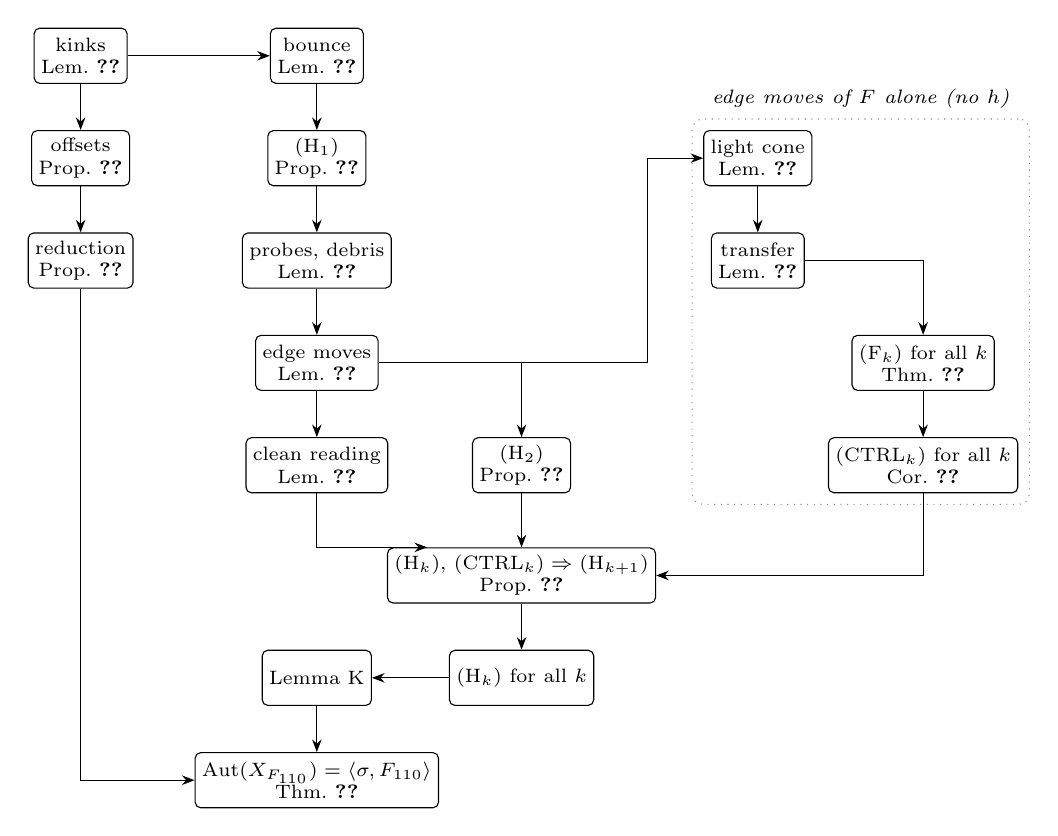
\begin{tikzpicture}[
  box/.style={draw, rounded corners=2pt, align=center, font=\scriptsize, inner sep=2.5pt, minimum height=7mm},
  comp/.style={box, dashed, fill=black!8},
  arr/.style={-{Stealth[length=1.6mm]}, thin},
  grp/.style={draw=black!45, dotted, rounded corners=4pt, inner sep=4pt}]
\node[box] (kinks) at (0,0) {kinks\\ Lem.~\ref{cl:lem:kinks}};
\node[box] (off) at (0,-1.3) {offsets\\ Prop.~\ref{cl:prop:offsets}};
\node[box] (red) at (0,-2.6) {reduction\\ Prop.~\ref{cl:prop:reduce}};
\node[box] (bounce) at (3,0) {bounce\\ Lem.~\ref{cl:lem:bounce}};
\node[box] (H1) at (3,-1.3) {$(\mathrm H_1)$\\ Prop.~\ref{cl:prop:H1}};
\node[box] (probe) at (3,-2.6) {probes, debris\\ Lem.~\ref{cl:lem:probe}};
\node[box] (moves) at (3,-3.9) {edge moves\\ Lem.~\ref{cl:lem:edgemove}};
\node[box] (clean) at (3,-5.2) {clean reading\\ Lem.~\ref{cl:lem:clean}};
\node[box] (H2) at (5.6,-5.2) {$(\mathrm H_2)$\\ Prop.~\ref{cl:prop:H2}};
\node[box] (cone) at (8.6,-1.3) {light cone\\ Lem.~\ref{cl:lem:movelocal}};
\node[box] (Rt) at (8.6,-2.6) {transfer\\ Lem.~\ref{cl:lem:transfer}};
\node[box] (Fk) at (10.7,-3.9) {$(\mathrm F_k)$ for all $k$\\ Thm.~\ref{cl:thm:Fk}};
\node[box] (ctrl) at (10.7,-5.2) {$(\mathrm{CTRL}_k)$ for all $k$\\ Cor.~\ref{cl:cor:ctrl}};
\node[box] (step) at (5.6,-6.6) {$(\mathrm H_k)$, $(\mathrm{CTRL}_k)\Rightarrow(\mathrm H_{k+1})$\\ Prop.~\ref{cl:prop:ctrlstep}};
\node[box] (Hk) at (5.6,-7.9) {$(\mathrm H_k)$ for all $k$};
\node[box] (K) at (3,-7.9) {Lemma K};
\node[box] (thm) at (3,-9.2) {$\Aut(X_{F_{110}})=\langle\sh,F_{110}\rangle$\\ Thm.~\ref{cl:thm:110rigid}};
\draw[arr] (kinks) -- (off);
\draw[arr] (off) -- (red);
\draw[arr] (kinks) -- (bounce);
\draw[arr] (bounce) -- (H1);
\draw[arr] (H1) -- (probe);
\draw[arr] (probe) -- (moves);
\draw[arr] (moves) -- (clean);
\draw[arr] (moves.east) -| (H2.north);
\draw[arr] (moves.east) -- (7.2,-3.9) |- (cone.west);
\draw[arr] (cone) -- (Rt);
\draw[arr] (Rt.east) -| (Fk.north);
\draw[arr] (Fk) -- (ctrl);
\draw[arr] (ctrl.south) |- (step.east);
\draw[arr] (clean.south) |- ([xshift=-12mm]step.north) ;
\draw[arr] (H2) -- (step);
\draw[arr] (step) -- (Hk);
\draw[arr] (Hk) -- (K);
\draw[arr] (K) -- (thm);
\draw[arr] (red) |- (thm.west);
\begin{scope}[on background layer]
\node[grp, fit=(cone)(Rt)(Fk)(ctrl), label={[font=\scriptsize\itshape]above:edge moves of $F$ alone (no $h$)}] {};
\end{scope}
\end{tikzpicture}
\caption{Dependencies in the proof for the class of $110$. Every step is proved by hand, for every $k$ and every radius. The boxes in the dotted frame concern the edge moves of $F$ alone and do not involve the block map $h$. For $42$ the same diagram applies with Theorem~\ref{cl:thm:Fk42}; for $46$ the controllability theorem is Theorem~\ref{cl:thm:Fk46}; for $66$ and $189$ the steps are those of Section~\ref{c24:sec}, with the controllability theorem for $46$ transported by the factor map $\delta$ (Lemma~\ref{c24:lem:moves46}); for $93$ the probes, moves and $(\mathrm H_2)$, $(\mathrm H_3)$ are replaced as described in Section~\ref{sec:79}, and the induction starts from Proposition~\ref{c79:prop:F3}, which describes the orbits of the moves at level $3$.}
\label{fig:dep}
\end{figure}


\subsection{Configurations that vanish to the right}\label{cl:sec:tail}

Call $c\in\A^{\Z}$ \emph{$0$-tailed} if $c\ne(0,0)^{\Z}$ and $c_i=(0,0)$ for all large $i$, and let $e(c)$ be the largest $i$ with $c_i\ne(0,0)$, the \emph{edge} of $c$. Recall that $(F^tc)_i=(Y_c(t-1,i),Y_c(t,i))$. Since $f(a,0,0)=0$ and $f(a,b,0)=b$, the columns of $Y_c$ to the right of $e=e(c)$ stay $0$ and column $e$ obeys $Y_c(t+1,e)=Y_c(t-1,e)\oplus Y_c(t,e)$; as this recurrence is reversible, $e(F^tc)=e(c)$ for all $t\in\Z$, and column $e$ runs through the cycle $\dots011011\dots$, never $0$ in two consecutive rows. Let $\mathcal H$ be the set of block maps $h$, of any radius and not necessarily invertible, that commute with $F$ and fix $\eta_0$ and $\rho\eta_0$. Such an $h$ commutes with $\sh$, so it fixes every $\eta_p$ and $\rho\eta_p$, and it fixes $(0,0)^{\Z}$, which $\eta_0$ contains far to the left; and $\rho h\rho\in\mathcal H$, because $\rho F\rho=F^{-1}$. For $k\ge1$ consider
\begin{itemize}
\item[$(\mathrm H_k)$] \emph{for every $h\in\mathcal H$ and every $0$-tailed $c$, $Y_{hc}(t,i)=Y_c(t,i)$ for all $t\in\Z$ and all $i\ge e(c)-k+1$.}
\end{itemize}
So $(\mathrm H_k)$ says that $hc=c$ on the columns $i\ge e(c)-k+1$ at all times; in particular $hc$ is $0$-tailed with $e(hc)=e(c)$. $(\mathrm H_{R+1})$ implies Lemma K for radius $R$: if $h\in\mathcal H$ has radius $R$ and $w\in\A^{2R+1}$ is not $(0,0)^{2R+1}$, let $c$ be $w$ on $[-R,R]$ and $(0,0)$ elsewhere; then $e(c)\le R$, so $h(w)=(hc)_0=c_0=w_0$; and $h((0,0)^{2R+1})=(0,0)$ because $h$ fixes $(0,0)^{\Z}$.

For $d$ with $d_i=(0,0)$ for $i>r$ and a configuration $\Lambda$ with $\Lambda_i=(0,0)$ for $i\le r$, write $d\sqcup\Lambda$ for the configuration equal to $d$ on $(-\infty,r]$ and to $\Lambda$ on $(r,\infty)$.

\subsection{Fronts and the edge column}\label{cl:sec:fronts}

Since $f(1,1,1)=0$, $F$ and $F^{-1}$ map a configuration that is $(1,1)$ far to the right to another such configuration, so every row of its diagram is $1$ far to the right. We say that such a $c$ has a \emph{front} at $(t_0,q)$ if $Y_c(t_0,q)=0$, $Y_c(t_0,i)=1$ for $i>q$, and $Y_c(t_0-1,i)=1$ for $i\ge q$. The kink $\eta_p$ has $Y_{\eta_p}(t,i)=[i>p+t]$, so it has a front at $(t,p+t)$ for every $t$; the kink $\rho\eta_N$ has $Y_{\rho\eta_N}(t,i)=[i\ge N-t]$, so the rightmost $0$ of its row $t$ is at $N-1-t$.

\begin{lemma}[zero wake and bounce]\label{cl:lem:bounce}
\begin{enumerate}
\item[(a)] If $c$ has a front at $(t_0,q)$, then for every $t\ge t_0$ row $t$ of $Y_c$ is $0$ on $[q,q+t-t_0]$ and $1$ on $(q+t-t_0,\infty)$, and $F^tc$ agrees with $\eta_{q+t-t_0}$ on $[q,\infty)$. So $c$ has a front at $(t,q+t-t_0)$ for every $t\ge t_0$, and the integer $U(c)=q-t_0$ does not depend on the front chosen: it is the eventual value of $\mu_t-t$, where $\mu_t$ is the largest $i$ with $Y_c(t,i)=0$. The kink $\rho\eta_N$ has no front.
\item[(b)] If $c$ has a front and $h\in\mathcal H$, then $hc$ has a front and $U(hc)=U(c)$.
\item[(c)] \emph{(Bounce.)} Let $d$ be $0$-tailed with $e(d)=e$, let $N\ge e+1$, and let $c=d\sqcup\rho\eta_N$, glued at $r=e$. Then $c$ has a front, and $U(c)=2e-N+\varphi$, where $\varphi=Y_d(N-e-1,e)$.
\end{enumerate}
\end{lemma}

\begin{proof}
(a) Write $Y=Y_c$ and $s=q+t-t_0$, and argue by induction on $t\ge t_0$; at $t=t_0$ the statement about row $t$ is the hypothesis, and row $t_0-1$ is $1$ on $[q,\infty)$. Assume the statement for rows $t-1$ and $t$, and compute row $t+1$ from $Y(t+1,i)=Y(t-1,i)\oplus f(Y(t,i-1),Y(t,i),Y(t,i+1))$. For $i>s+1$ it is $1\oplus f(1,1,1)=1$; for $i=s+1$ it is $1\oplus f(0,1,1)=0$; for $i=s$ it is $1\oplus f(Y(t,s-1),0,1)=0$, since $f(a,0,1)=1$; and for $q\le i<s$ it is $0\oplus f(Y(t,i-1),0,0)=0$, since $f(a,0,0)=0$. As $Y_{\eta_p}(-1,i)=[i\ge p]$ and $Y_{\eta_p}(0,i)=[i>p]$, rows $t-1$ and $t$ are those of $\eta_{s}$ on $[q,\infty)$. So $\mu_t=t+q-t_0$ for $t\ge t_0$, which gives the independence of $U$. For $\rho\eta_N$, $\mu_t=N-1-t$ is decreasing, so it is not of the form $t+U$ for all large $t$.

(b) Let $R$ be the radius of $h$. Since $h$ fixes $\eta_0$, which is $(1,1)$ far to the right, it maps the window $(1,1)^{2R+1}$ to $(1,1)$, so $hc$ is $(1,1)$ far to the right. Let $c$ have a front at $(t_0,q)$, let $t\ge t_0+R$ and $p=q+t-t_0\ge q+R$. By (a), $F^tc$ agrees with $\eta_p$ on $[q,\infty)$, so $F^thc=hF^tc$ agrees with $h\eta_p=\eta_p$ on $[q+R,\infty)$, which contains $p$. Hence $hc$ has a front at $(t,p)$, and $U(hc)=p-t=U(c)$. No inverse of $h$ is used.

(c) Put $Y=Y_c$ and $t_0=N-e-1\ge0$. The configurations $c$ and $d$ agree on $(-\infty,N-1]$, and $F^{\pm1}$ have radius $1$, so the states of $c$ and $d$ at time $t\ge0$ agree on $(-\infty,N-1-t]$; at $t=t_0$ this is $(-\infty,e]$. On $(e,\infty)$, row $t$ of $Y$ is $[i\ge N-t]$, as for $\rho\eta_N$, for $-1\le t\le t_0$: this holds for $t=-1,0$, and for $1\le t+1\le t_0$ the only entry of row $t+1$ on $(e,\infty)$ that reads a column $\le e$ is the one at $e+1$, which is $Y(t-1,e+1)\oplus f(Y(t,e),Y(t,e+1),Y(t,e+2))$ with $Y(t,e+1)=0$, as $e+1<N-t$; and $f(a,0,c)=c$ does not read $a$. So row $t_0$ is $1$ on $(e,\infty)$, row $t_0-1$ is $0$ at $e+1$ and $1$ on $[e+2,\infty)$, $Y(t_0,e)=\varphi$ and $Y(t_0-1,e)=Y_d(t_0-1,e)$. Row $t_0+1$ is $1\oplus f(1,1,1)=1$ on $[e+2,\infty)$ and $0\oplus f(\varphi,1,1)=\neg\varphi$ at $e+1$.

If $\varphi=1$, then $c$ has a front at $(t_0+1,e+1)$, and $U(c)=e+1-(t_0+1)=2e-N+1$. If $\varphi=0$, then $Y(t_0-1,e)=1$, because the edge column of $d$ is never $0$ in two consecutive rows, so $Y(t_0+1,e)=1\oplus f(Y(t_0,e-1),0,1)=0$, and row $t_0+1$ is $1$ on $[e+1,\infty)$. Then $Y(t_0+2,e+1)=1\oplus f(0,1,1)=0$ and $Y(t_0+2,i)=1\oplus f(1,1,1)=1$ for $i\ge e+2$, so $c$ has a front at $(t_0+2,e+1)$, and $U(c)=e+1-(t_0+2)=2e-N$.
\end{proof}

\figinc[0.6\textwidth]{fig_front}{A front for rule $110$ (Lemma~\ref{cl:lem:bounce}(a)): the diagram of a configuration that is $(1,1)$ to the right of a random block. From the front at $(t_0,q)$ on, row $t$ is $0$ on $[q,q+t-t_0]$ and $1$ beyond, and the front moves to the right at speed $1$. Time increases upwards; black cells are $1$.}{fig:front}

\figinc[0.5\textwidth]{fig_bounce}{The bounce of Lemma~\ref{cl:lem:bounce}(c) for rule $110$: the diagram of $d\sqcup\rho\eta_N$, with $d$ a random $0$-tailed configuration with edge $e$ (marked). The kink $\rho\eta_N$ enters from the right, meets the edge column at time $N-e-1$ and leaves as a front of speed $1$, whose position $U=2e-N+\varphi$ records one value $\varphi$ of the edge column. Time increases upwards; black cells are $1$.}{fig:bounce}

\begin{proposition}[$(\mathrm H_1)$]\label{cl:prop:H1}
For every $h\in\mathcal H$ and every $0$-tailed $d$, the configuration $hd$ is $0$-tailed with $e(hd)=e(d)$, and $Y_{hd}(t,i)=Y_d(t,i)$ for all $t\in\Z$ and all $i\ge e(d)$. That is, $(\mathrm H_1)$ holds.
\end{proposition}

\begin{proof}
Let $R$ be the radius of $h$, $e=e(d)$, $N\ge e+2R+1$, and $c=d\sqcup\rho\eta_N$, glued at $e$. Since $h$ fixes $(0,0)^{\Z}$, $(hd)_i=(0,0)$ for $i>e+R$. For $i\le N-R-1$ the window of $i$ lies in $(-\infty,N-1]$, where $c=d$, so $(hc)_i=(hd)_i$; for $i\ge e+R+1$ it lies in $(e,\infty)$, where $c=\rho\eta_N$, so $(hc)_i=(h\rho\eta_N)_i=(\rho\eta_N)_i$. These ranges cover $\Z$, and on their overlap both $hd$ and $\rho\eta_N$ are $(0,0)$. So $hc=\rho\eta_N$ if $hd=(0,0)^{\Z}$; otherwise $hd$ is $0$-tailed with $e'=e(hd)\le e+R<N$, and $hc=hd\sqcup\rho\eta_N$, glued at $e'$. By Lemma~\ref{cl:lem:bounce}(c), $c$ has a front, so by part~(b) of that lemma $hc$ has a front and $U(hc)=U(c)$; by part~(a), $\rho\eta_N$ has none, so $hd\ne(0,0)^{\Z}$. Part~(c), for $c$ and for $hc$, now gives
\[
2e'-N+Y_{hd}(N-e'-1,e')=2e-N+Y_d(N-e-1,e).
\]
So $2(e'-e)\in\{-1,0,1\}$, hence $e'=e$, and then $Y_{hd}(s,e)=Y_d(s,e)$ for every $s=N-e-1\ge2R$. Both edge columns obey the reversible recurrence $Y(t+1,e)=Y(t-1,e)\oplus Y(t,e)$, so they agree at all times. To the right of $e$ both diagrams vanish, since $e(F^thd)=e(F^td)=e$ for all $t$.
\end{proof}

\subsection{Probes and edge moves}\label{cl:sec:probes}

\begin{lemma}[probes and debris]\label{cl:lem:probe}
Let $h\in\mathcal H$ have radius $R$, let $c$ be $0$-tailed with $e(c)=r$, put $Y=Y_c$, and for $n\in\Z$ let $P_n(c)=F^{-n}(F^nc\sqcup\rho\eta_{r+2})$, the \emph{probe} of $c$ at time $n$.
\begin{enumerate}
\item[(a)] $F^nP_n(c)=F^j(F^{n-j}c\sqcup\rho\eta_{r+2+j})$ for every $j\ge0$, and $hP_n(c)=P_n(hc)$.
\item[(b)] Let $\varepsilon=1$ if $Y(n+1,r)=0$ and $\varepsilon=0$ otherwise. There is a unique $0$-tailed configuration $D=D_n(c)$, the \emph{debris}, with $e(D)=r$ such that
\[
F^sP_n(c)=F^sD\sqcup\eta_{r+s-n-1-\varepsilon}\qquad\text{for all }s\ge n+2+\varepsilon.
\]
The diagrams of $D$ and of $P=P_n(c)$ agree on the columns $\le r$ at all rows $\ge n+1+\varepsilon$. On the columns $\le r$, the diagram of $P$ equals $Y$ at the rows $n-1$, $n$, $n+1$; at row $n+2$ it equals $Y$ on the columns $\le r-1$. If $\varepsilon=1$, then $Y_P(n+2,r)=0$ and $Y_P(n+3,r)=1$. Finally $hD_n(c)=D_n(hc)$.
\item[(c)] $\rho$ maps $0$-tailed configurations to $0$-tailed configurations with the same edge, $Y_{\rho c}(t,i)=Y_c(-1-t,i)$, and $\rho h\rho\in\mathcal H$.
\end{enumerate}
\end{lemma}

The configuration $F^nc\sqcup\rho\eta_{r+2}$ is the state at time $n$ of $c$ with a kink glued next to its edge; by (b), after time $n+2+\varepsilon$ the glued configuration splits into the debris and an outgoing kink $\eta$, and the debris differs from $c$ only near the edge (Figure~\ref{fig:probe}). The statements about $h$ use $(\mathrm H_1)$, which holds by Proposition~\ref{cl:prop:H1}.

\begin{proof}
Two gluing facts. (i) If $d_i=(0,0)$ for $i>r$, then $F(d\sqcup\eta_N)=Fd\sqcup\eta_{N+1}$ for $N\ge r+1$, and $F(d\sqcup\rho\eta_N)=Fd\sqcup\rho\eta_{N-1}$ for $N\ge r+3$. Indeed the $y$-component at $r+1$ is $0$ in both glued configurations, so the cells $i\le r$ evolve as in $Fd$; the cells $i\ge r+2$ read only cells $\ge r+1$, which are those of the kink; and the new cell $r+1$ is $(0,0)$, because $f(a,0,0)=0$ and $f(a,0,1)=1$ do not depend on $a$ (for $\eta_N$ the cell $r+1$ is $(1,0)$ if $N=r+1$ and $(0,0)$ otherwise; for $\rho\eta_N$, $N\ge r+3$, the cells $r+1$, $r+2$ are $(0,0)$). Then use $F\eta_N=\eta_{N+1}$ and $F\rho\eta_N=\rho\eta_{N-1}$ (Lemma~\ref{cl:lem:kinks}). (ii) If moreover $(hd)_i=(0,0)$ for $i>r$ and $\Lambda\in\{\eta_N,\rho\eta_N\}$ with $N\ge r+2R+1$, then $h(d\sqcup\Lambda)=hd\sqcup\Lambda$: for $i\le N-R-1$ the window of $i$ lies where $d\sqcup\Lambda=d$, and for $i\ge r+R+1$ it lies where $d\sqcup\Lambda=\Lambda$, and $h\Lambda=\Lambda$; these ranges cover $\Z$, and on $(r,N)$ both $hd$ and $\Lambda$ are $(0,0)$.

(a) The identity is (i) applied $j$ times. Take $j\ge 2R-1$. By Proposition~\ref{cl:prop:H1}, $hF^{n-j}c=F^{n-j}hc$ vanishes to the right of $r$, so by (ii), $h(F^{n-j}c\sqcup\rho\eta_{r+2+j})=F^{n-j}hc\sqcup\rho\eta_{r+2+j}$; apply $F^{j-n}$, which commutes with $h$.

(b) Write $P=P_n(c)$. Rows $n-1$ and $n$ of $Y_P$ are the two rows of $F^nP=F^nc\sqcup\rho\eta_{r+2}$: on the columns $\le r$ they are $Y(n-1,\cdot)$ and $Y(n,\cdot)$; row $n-1$ is $0$ at $r+1,r+2$ and $1$ beyond, and row $n$ is $0$ at $r+1$ and $1$ beyond. By the relation, row $n+1$ of $Y_P$ is $Y(n+1,\cdot)$ on the columns $\le r$, because $Y_P(n,r+1)=0=Y(n,r+1)$, and it is $1$ on the columns $>r$ (at $r+1$ it is $0\oplus f(Y(n,r),0,1)=1$, at $r+2$ it is $0\oplus f(0,1,1)=1$, and beyond $1\oplus f(1,1,1)=1$). Row $n+2$ is $1\oplus f(1,1,1)=1$ on the columns $\ge r+2$ and $0\oplus f(Y(n+1,r),1,1)=\neg Y(n+1,r)=\varepsilon$ at $r+1$; on the columns $\le r-1$ it reads only columns $\le r$ of rows $n$, $n+1$, so it equals $Y(n+2,\cdot)$ there.

If $\varepsilon=0$, the state $F^{n+2}P$ has the cell $(1,0)$ at $r+1$ and $(1,1)$ beyond, so $F^{n+2}P=d\sqcup\eta_{r+1}$, where $d$ agrees with $F^{n+2}P$ on $(-\infty,r]$ and vanishes beyond; its cell $r$ is $(Y(n+1,r),\cdot)=(1,\cdot)\ne(0,0)$. If $\varepsilon=1$, then $Y(n+1,r)=0$, so $Y(n,r)=1$ because the edge column of $c$ is never $0$ twice in a row, and $Y_P(n+2,r)=Y(n,r)\oplus f(Y(n+1,r-1),0,1)=0$. Then $Y_P(n+3,r+1)=Y_P(n+1,r+1)\oplus f(0,1,1)=0$, $Y_P(n+3,i)=1$ for $i\ge r+2$, and $Y_P(n+3,r)=Y_P(n+1,r)\oplus f(Y_P(n+2,r-1),0,1)=1$. So $F^{n+3}P=d\sqcup\eta_{r+1}$ with cell $r$ of $d$ equal to $(0,1)$. In both cases put $D=F^{-(n+2+\varepsilon)}d$; it is $0$-tailed with $e(D)=r$, and (i) gives $F^sP=F^sD\sqcup\eta_{r+s-n-1-\varepsilon}$ for $s\ge n+2+\varepsilon$. Rows $s-1$ and $s$ of a diagram are the two rows of the state at time $s$, so the diagrams of $D$ and $P$ agree on the columns $\le r$ at all rows $\ge n+1+\varepsilon$. If $D'$ is $0$-tailed with $e(D')=r$ and $F^sP=F^sD'\sqcup\eta_{N'}$ for some $s$ and some $N'\ge r+1$, then by (i), applied to $F^sD'$, which vanishes to the right of $r$, $F^{s'}P=F^{s'}D'\sqcup\eta_{N'+s'-s}$ for every $s'\ge s$; for $s'\ge\max(s,n+2+\varepsilon)$, $F^{s'}D'$ and $F^{s'}D$ both agree with $F^{s'}P$ on $(-\infty,r]$ and vanish beyond, so $F^{s'}D'=F^{s'}D$ and $D'=D$; this is the uniqueness.

By Proposition~\ref{cl:prop:H1}, $c'=hc$ is $0$-tailed with $e(c')=r$ and $Y_{c'}(n+1,r)=Y(n+1,r)$, so $c'$ has the same $\varepsilon$. For $s$ so large that $N=r+s-n-1-\varepsilon\ge r+2R+1$, (a), (ii) and Proposition~\ref{cl:prop:H1} for $F^sD$ give $F^sD_n(c')\sqcup\eta_N=F^sP_n(c')=hF^sP=hF^sD\sqcup\eta_N$, hence $F^sD_n(c')=F^shD$ and $hD=D_n(c')$.

(c) $\rho$ exchanges the two rows of every cell, which with $F^t\rho=\rho F^{-t}$ gives the formula for $Y_{\rho c}$; and $\rho h\rho$ commutes with $F$ since $\rho F\rho=F^{-1}$, and fixes $\rho\eta_0$ and $\eta_0$.
\end{proof}

\figinc[\textwidth]{fig_probe}{A probe and its debris for rule $110$ (Lemma~\ref{cl:lem:probe}). Left: the diagram of the probe $P_n(c)$; the kink glued at time $n$ next to the edge column $r$ leaves as an outgoing kink $\eta$. Right: the debris $D_n(c)$. Here $n=2$ and $\varepsilon=1$; for $s\ge n+2+\varepsilon$, $F^sP_n(c)=F^sD_n(c)\sqcup\eta_{r+s-n-1-\varepsilon}$. On the columns $\le r$ the two diagrams differ only in the shaded cells, all at rows $\le n+\varepsilon$.}{fig:probe}

\emph{Edge moves.} A probe followed by passage to its debris changes a configuration only at its edge cell, at a single time; so does its conjugate by $\rho$; and $h$ commutes with both. For a $0$-tailed $b$ with $e(b)=r$ and $m\in\Z$ write the cells of the state $F^mb$ as $(F^mb)_i=(x_i,y_i)$, so that $x_i=Y_b(m-1,i)$, $y_i=Y_b(m,i)$, and the edge cell is $(x_r,y_r)\ne(0,0)$.

\begin{lemma}[edge moves]\label{cl:lem:edgemove}
Let $b$ be $0$-tailed with $e(b)=r$, let $m\in\Z$, and let $(x_i,y_i)$ be the cells of $F^mb$. Put $M_m(b)=D_{m-2}(b)$ and $\bar M_m(b)=\rho D_{-m-2}(\rho b)$.
\begin{enumerate}
\item[(a)] $M_m(b)$ is $0$-tailed with edge $r$, and $F^mM_m(b)$ agrees with $F^mb$ at every cell except the edge cell, where $(x_r,y_r)$ becomes $(1,0)$ if $(x_r,y_r)=(0,1)$, and becomes $(1,y_r\oplus x_{r-1})$ if $x_r=1$.
\item[(b)] $\bar M_m(b)$ is $0$-tailed with edge $r$, and $F^m\bar M_m(b)$ agrees with $F^mb$ at every cell except the edge cell, where $(x_r,y_r)$ becomes $(0,1)$ if $(x_r,y_r)=(1,0)$, and becomes $(x_r\oplus y_{r-1},1)$ if $y_r=1$.
\item[(c)] $hM_m=M_mh$ and $h\bar M_m=\bar M_mh$ on $0$-tailed configurations with edge $r$, for every $h\in\mathcal H$ and every $m\in\Z$.
\end{enumerate}
\end{lemma}

So, at any time $m$ and in the notation $x_ry_r$ for the edge cell, the \emph{moves} are $01\to10$ and $10\to01$, always; $1y\to1\bar y$ if $x_{r-1}=1$; and $x1\to\bar x1$ if $y_{r-1}=1$. In the remaining cases (a) and (b) leave $b$ unchanged. By (a) and (b), $M_m$ and $\bar M_m$ are described by their effect on the state at time $m$ alone, without reference to any $h$. Part~(c) is an identity of operators: a composite $O$ of moves is a fixed map, and $hO=Oh$, although the effect of each move depends on the configuration to which it is applied.

\begin{proof}
(a) Put $n=m-2$, $Y=Y_b$, $P=P_n(b)$ and $D=D_n(b)$, and let $\varepsilon$ be as in Lemma~\ref{cl:lem:probe}(b), so $\varepsilon=1$ exactly when $x_r=Y(m-1,r)=0$. By that lemma $D$ is $0$-tailed with $e(D)=r$, and the diagram of $P$ equals $Y$ on the columns $\le r$ at the rows $m-3,m-2,m-1$, and at row $m$ on the columns $\le r-1$; at $(m,r)$ it is $Y(m-2,r)\oplus f(x_{r-1},x_r,1)$, while $y_r=Y(m-2,r)\oplus f(x_{r-1},x_r,0)=Y(m-2,r)\oplus x_r$.

If $x_r=1$, then $\varepsilon=0$, so the diagrams of $D$ and $P$ agree on the columns $\le r$ at the rows $\ge m-1$. Hence rows $m-1$, $m$ of $D$ are $x$ and $y$ on the columns $\le r$, except that $Y_D(m,r)=Y(m-2,r)\oplus f(x_{r-1},1,1)=Y(m-2,r)\oplus\neg x_{r-1}=y_r\oplus x_{r-1}$. If $x_r=0$, then $y_r=1$, $\varepsilon=1$, and the diagrams of $D$ and $P$ agree on the columns $\le r$ at the rows $\ge m$. Row $m$ of $D$ is that of $P$: it is $y_i$ for $i\le r-1$ and $Y_P(m,r)=0$ at $r$. Row $m-1$ of $D$ follows from rows $m$ and $m+1$ by the relation solved for the earlier row: for $i\le r-1$ the relation reads only columns $\le r$ of these rows, so $Y_D(m-1,i)=Y_P(m-1,i)=x_i$; and, as $Y_D(m,r+1)=0$, $Y_D(m-1,r)=Y_D(m+1,r)\oplus f(y_{r-1},0,0)=Y_P(m+1,r)=1$, the value at $(n+3,r)$ in Lemma~\ref{cl:lem:probe}(b). So the edge cell becomes $(1,0)$ and nothing else changes. In both cases the cells $i>r$ are $(0,0)$ since $e(D)=r$.

(b) By Lemma~\ref{cl:lem:probe}(c), $\rho b$ is $0$-tailed with edge $r$ and $Y_{\rho b}(t,i)=Y_b(-1-t,i)$, so the state of $\rho b$ at time $-m$ has the rows $Y_{\rho b}(-m-1,\cdot)=y$ and $Y_{\rho b}(-m,\cdot)=x$. Apply (a) to $\rho b$ at time $-m$, that is $M_{-m}(\rho b)=D_{-m-2}(\rho b)$, with the roles of $x$ and $y$ exchanged, and then $\rho$, which turns the state at time $-m$ back into the state at time $m$ with its two rows exchanged.

(c) By Proposition~\ref{cl:prop:H1}, $hb$ is again $0$-tailed with edge $r$. Lemma~\ref{cl:lem:probe}(b) gives $hD_n(b)=D_n(hb)$ for every $n$, which is $hM_m=M_mh$. Since $\rho h\rho\in\mathcal H$, the same lemma gives $(\rho h\rho)D_n=D_n(\rho h\rho)$, and therefore $h\bar M_m(b)=\rho(\rho h\rho)D_{-m-2}(\rho b)=\rho D_{-m-2}(\rho hb)=\bar M_m(hb)$.
\end{proof}

\subsection{The second column and the inductive step}\label{cl:sec:step}

\begin{proposition}[$(\mathrm H_2)$]\label{cl:prop:H2}
$(\mathrm H_2)$ holds.
\end{proposition}

\begin{proof}
Let $h\in\mathcal H$, let $c$ be $0$-tailed with $e(c)=r$, and put $Y=Y_c$ and $G=Y_{hc}\oplus Y$. By Proposition~\ref{cl:prop:H1}, $G$ vanishes on the columns $\ge r$, and it remains to show that $G(t,r-1)=0$ for every $t$.

(a) Suppose $Y(t,r)=1$, and put $m=t+1$, so that the state at time $m$ has the rows $t$ and $t+1$ and its edge cell has $x_r=Y(t,r)=1$. By Lemma~\ref{cl:lem:edgemove}(a), $b=M_mc$ has $Y_b(t+1,r)=Y(t+1,r)\oplus Y(t,r-1)$. By Proposition~\ref{cl:prop:H1}, $Y_{hc}(t,r)=1$ and $Y_{hc}(t+1,r)=Y(t+1,r)$, so the same lemma gives $Y_{M_mhc}(t+1,r)=Y(t+1,r)\oplus Y_{hc}(t,r-1)$. By Lemma~\ref{cl:lem:edgemove}(c), $M_mhc=hb$, and by Proposition~\ref{cl:prop:H1} for $b$, which is $0$-tailed with edge $r$, $Y_{hb}(t+1,r)=Y_b(t+1,r)$. Comparing, $Y_{hc}(t,r-1)=Y(t,r-1)$, that is, $G(t,r-1)=0$.

(b) Suppose $Y(t,r)=0$. Then $Y(t\pm1,r)=1$, since the edge column runs through the cycle $\dots011011\dots$, so $G(t\pm1,r-1)=0$ by (a). Since $f(a,b,0)=b$ and $Y_{hc}(t,r)=Y(t,r)=0$, the relation at $(t,r-1)$ reads $Y(t+1,r-1)\oplus Y(t-1,r-1)=Y(t,r-1)$ in both diagrams, so $G(t,r-1)=G(t+1,r-1)\oplus G(t-1,r-1)=0$.
\end{proof}

\begin{lemma}[clean reading]\label{cl:lem:clean}
Let $k\ge2$ and assume $(\mathrm H_k)$. Let $h\in\mathcal H$, let $b$ be $0$-tailed with $e(b)=r$, and let $O$ be a finite composite of moves $M_m$, $\bar M_m$ with $|m|\le k-1$. Then $Y_{Ob}(0,i)=Y_b(0,i)$ and $Y_{Ohb}(0,i)=Y_{hb}(0,i)$ for $i\le r-k$. If moreover $Y_{Ob}(0,r-k+1)=Y_{Ob}(0,r-k+2)=1$, then $Y_{hb}(0,r-k)=Y_b(0,r-k)$.
\end{lemma}

\begin{proof}
A move at time $m$ changes the state at time $m$ only at column $r$. Since $F$ and $F^{-1}$ have radius $1$, the states at time $0$ before and after the move differ only on columns $\ge r-|m|\ge r-k+1$, so row $0$ is unchanged on columns $\le r-k$. Applying this to each factor of $O$ in turn, starting from $b$ or from $hb$, which is $0$-tailed with edge $r$ by Proposition~\ref{cl:prop:H1}, gives the first statement. Put $Y=Y_{Ob}$ and $G'=Y_{hOb}\oplus Y$. By Lemma~\ref{cl:lem:edgemove}(c), $hOb=Ohb$, so $G'(0,r-k)=Y_{Ohb}(0,r-k)\oplus Y_{Ob}(0,r-k)=Y_{hb}(0,r-k)\oplus Y_b(0,r-k)$. Since $Ob$ is $0$-tailed with edge $r$, $(\mathrm H_k)$ gives $G'=0$ on columns $\ge r-k+1$ at all times. The relation \eqref{cl:eq:G} for $G'$ at $(0,r-k+1)$ then reads
\[
0=f\bigl(Y(0,r-k)\oplus G'(0,r-k),1,1\bigr)\oplus f\bigl(Y(0,r-k),1,1\bigr),
\]
where we used $Y(0,r-k+1)=Y(0,r-k+2)=1$ and $r-k+2\le r$. As $f(a,1,1)=\neg a$, $G'(0,r-k)=0$.
\end{proof}

For $k\ge1$ consider the following statement about $F_{110}$ alone; by the remark after Lemma~\ref{cl:lem:edgemove} it involves no $h$.
\begin{itemize}
\item[$(\mathrm{CTRL}_k)$] \emph{for every $0$-tailed $c$, with $r=e(c)$, there is a finite composite $O$ of moves $M_m$, $\bar M_m$ with $|m|\le k-1$ such that $Y_{Oc}(0,r-k+1)=Y_{Oc}(0,r-k+2)=1$.}
\end{itemize}

\begin{proposition}\label{cl:prop:ctrlstep}
For $k\ge2$, $(\mathrm{CTRL}_k)$ and $(\mathrm H_k)$ imply $(\mathrm H_{k+1})$.
\end{proposition}

\begin{proof}
Let $h\in\mathcal H$, let $c$ be $0$-tailed with $e(c)=r$, and let $t\in\Z$. Then $F^tc$ is $0$-tailed with edge $r$, and $(\mathrm{CTRL}_k)$ applied to $F^tc$ and Lemma~\ref{cl:lem:clean} with $b=F^tc$ give $Y_{hF^tc}(0,r-k)=Y_{F^tc}(0,r-k)$. Since $hF^t=F^th$ and $Y_{F^tc}(0,i)=Y_c(t,i)$, this is $Y_{hc}(t,r-k)=Y_c(t,r-k)$. Together with $(\mathrm H_k)$ this is $(\mathrm H_{k+1})$.
\end{proof}

\subsection{The controllability theorem}\label{cl:sec:ctrl}

The orbits of the moves can be determined exactly. Recall that $c_i=(Y_c(-1,i),Y_c(0,i))$: the state at time $0$ is $c$ itself. For $k\ge1$ and a $0$-tailed $c$ with $e(c)=r$, let $\mathcal O_k(c)$ be the set of configurations $Oc$, where $O$ ranges over the finite composites of moves $M_m$, $\bar M_m$ with $|m|\le k-1$; we call $c_{r-k+1}$ the \emph{tip} and $c_{r-k}$ the \emph{exterior cell} of $c$ at level $k$.

\begin{lemma}[light cone]\label{cl:lem:movelocal}
Let $b$ be $0$-tailed with $e(b)=r$, let $m\in\Z$, and let $b'$ be the image of $b$ under $M_m$ or $\bar M_m$.
\begin{enumerate}
\item[(a)] $b'$ is $0$-tailed with $e(b')=r$, and for $i\le r$, $Y_{b'}(t,i)\ne Y_b(t,i)$ only if $t-m\ge r-i$ or $m-1-t\ge r-i$. In particular $b'$ agrees with $b$ outside $[r-|m|,r]$.
\item[(b)] $b$ is the image of $b'$ under $M_m$ or $\bar M_m$. If $(x_r,y_r)$ is the edge cell of the state at time $m$ and $(x_{r-1},y_{r-1})$ the cell to its left, the moves at time $m$ always connect $x_ry_r=01$ with $10$, and they connect $11$ with $01$ or $10$ if and only if $(x_{r-1},y_{r-1})\ne(0,0)$.
\end{enumerate}
\end{lemma}

\begin{proof}
(a) By Lemma~\ref{cl:lem:edgemove}, the move changes the state at time $m$ only in its edge cell, which stays $\ne(0,0)$, so $b'$ is $0$-tailed with edge $r$. Since $F^{\pm1}$ have radius $1$, the state at time $m+s$ changes only on the columns $\ge r-|s|$; row $t$ is the second row of the state at time $t$ and the first row of the state at time $t+1$, which gives the cone, and at $t=-1,0$ the columns $\ge r-|m|$ (Figure~\ref{fig:cone}).

(b) This is the description of the moves after Lemma~\ref{cl:lem:edgemove}: $01\to10$ under $M_m$ and $10\to01$ under $\bar M_m$ are inverse to each other, and $1y\to1\bar y$ (when $x_{r-1}=1$) and $x1\to\bar x1$ (when $y_{r-1}=1$) are involutions, since a move does not change the cell $(x_{r-1},y_{r-1})$.
\end{proof}

\figinc[0.45\textwidth]{fig_cone}{The light cone of a move (Lemma~\ref{cl:lem:movelocal}(a)) for rule $110$: the diagrams of $b$ and of $M_mb$ for $m=3$ differ only at the highlighted cells, which lie in the cone $\{t-m\ge r-i\}\cup\{m-1-t\ge r-i\}$ below the edge column $r$; at time $0$ the change is confined to $[r-|m|,r]$.}{fig:cone}

By (b), $\mathcal O_k(c)$ is the class of $c$ under the equivalence relation generated by single moves at the times $|m|\le k-1$; in particular $\mathcal O_k(b)=\mathcal O_k(c)$ for $b\in\mathcal O_k(c)$, and $\mathcal O_{k-1}(c)\subseteq\mathcal O_k(c)$. By (a), every element of $\mathcal O_k(c)$ agrees with $c$ outside $[r-k+1,r]$.

The moves at the times $|m|\le k-1$ contain three families of moves of level $k-1$: those at the times $|m|\le k-2$, applied to $b$ itself, which change only the cells $r-k+2,\dots,r$; and the same moves applied to $Fb$ and to $F^{-1}b$, which can change the tip of $b$. The next lemma says how. It uses nothing about $f$ beyond Lemma~\ref{cl:lem:edgemove}(a),(b).

\begin{lemma}[transfer]\label{cl:lem:transfer}
Let $k\ge2$, let $b$ be $0$-tailed with $e(b)=r$, write $b_{r-k+j}=(u_j,v_j)$ for $j=0,1,2$, and put $v_3=Y_b(0,r-k+3)$, so that $v_3=0$ if $k=2$. By Section~\ref{cl:sec:tail}, $Fb$ is $0$-tailed with $e(Fb)=r$, so that $\mathcal O_{k-1}(Fb)$ is defined.
\begin{enumerate}
\item[(a)] $F^jM_m=M_{m-j}F^j$ and $F^j\bar M_m=\bar M_{m-j}F^j$ for all $j,m\in\Z$, and $\rho M_m\rho=\bar M_{-m}$. Consequently $F^{-1}\mathcal O_{k-1}(Fb)\subseteq\mathcal O_k(b)$ and $\rho\,\mathcal O_k(b)=\mathcal O_k(\rho b)$.
\item[(b)] The exterior cell of $Fb$ and its tip at level $k-1$ are $(v_1,\alpha)$ and $(v_2,\beta)$, where
\[
\alpha=u_1\oplus f(v_0,v_1,v_2),\qquad \beta=u_2\oplus f(v_1,v_2,v_3).
\]
\item[(c)] Let $\tilde b$ agree with $Fb$ outside $[r-k+2,r]$, and let $w$ be the $x$-bit of $\tilde b_{r-k+2}$. Then $b'=F^{-1}\tilde b$ agrees with $b$ on $(-\infty,r-k]$, and
\[
b'_{r-k+1}=\bigl(\alpha\oplus f(v_0,v_1,w),\ v_1\bigr).
\]
\end{enumerate}
\end{lemma}

\begin{proof}
(a) By Lemma~\ref{cl:lem:edgemove}(a), $F^mM_m(b)$ is obtained from $F^mb$ by a change of the edge cell that is a function of the cells $r-1$ and $r$ of $F^mb$ alone. Applied to $F^jb$ at the time $m-j$, the same description says that $F^{m-j}M_{m-j}(F^jb)$ is obtained in the same way from $F^{m-j}F^jb=F^mb$; so $F^{m-j}M_{m-j}F^jb=F^mM_mb$, that is, $M_{m-j}F^j=F^jM_m$. The same argument with Lemma~\ref{cl:lem:edgemove}(b) applies to $\bar M_m$. By definition, $\bar M_{-m}(b)=\rho D_{m-2}(\rho b)=\rho M_m(\rho b)$. If $\tilde b=O'Fb$ for a composite $O'$ of moves at the times $|m|\le k-2$, then $F^{-1}\tilde b=F^{-1}O'Fb$ is the image of $b$ under the corresponding composite of moves at the times $m+1$, and $|m+1|\le k-1$. Finally, conjugation by $\rho$ maps the set of moves at the times $|m|\le k-1$ onto itself.

(b) The cell $i$ of $Fb$ is $(Y_b(0,i),Y_b(1,i))$, and $Y_b(1,i)=Y_b(-1,i)\oplus f(Y_b(0,i-1),Y_b(0,i),Y_b(0,i+1))$; take $i=r-k+1$ and $i=r-k+2$.

(c) Since $\tilde b=Fb'$, the cell $i$ of $\tilde b$ is $(Y_{b'}(0,i),Y_{b'}(1,i))$. For $i\le r-k+1$ it equals the cell $i$ of $Fb$, so $Y_{b'}(0,i)=Y_b(0,i)$ and $Y_{b'}(1,i)=Y_b(1,i)$; and $Y_{b'}(0,r-k+2)=w$. Hence $Y_{b'}(-1,i)=Y_{b'}(1,i)\oplus f\bigl(Y_{b'}(0,i-1),Y_{b'}(0,i),Y_{b'}(0,i+1)\bigr)$ equals $Y_b(-1,i)$ for $i\le r-k$, and at $i=r-k+1$ it is $Y_b(1,r-k+1)\oplus f(v_0,v_1,w)=\alpha\oplus f(v_0,v_1,w)$, by (b).
\end{proof}

\begin{theorem}\label{cl:thm:Fk}
Let $k\ge1$ and let $c$ be $0$-tailed with $e(c)=r$. Then $\mathcal O_k(c)$ is the set $\mathcal S_k(c)$ of configurations $c'$ with
\begin{enumerate}
\item[(i)] $c'_i=c_i$ for every $i\notin[r-k+1,r]$, and $c'_r\ne(0,0)$; and
\item[(ii)] if the exterior cell $c_{r-k}$ is $(0,0)$, then $c'_{r-k+1}=(1,1)$ if and only if $c_{r-k+1}=(1,1)$.
\end{enumerate}
In words: the moves at the times $|m|\le k-1$ reach every configuration that agrees with $c$ outside the $k$ cells ending at the edge and whose edge cell is not $(0,0)$, except that a tip $(1,1)$, and the absence of one, cannot be changed when the exterior cell is $(0,0)$.
\end{theorem}

We call the statement of the theorem for a given $k$ $(\mathrm F_k)$. The constraints (i) and (ii) are invariant (Lemma~\ref{cl:lem:Finv}); $(\mathrm F_1)$ is immediate; and $(\mathrm F_{k-1})$ implies $(\mathrm F_k)$ for every $k\ge2$, by applying $(\mathrm F_{k-1})$ to $b$, to $Fb$ and to $F^{-1}b$, the last two through Lemma~\ref{cl:lem:transfer}.

\begin{lemma}[invariance]\label{cl:lem:Finv}
Every $c'\in\mathcal O_k(c)$ satisfies (i) and (ii).
\end{lemma}

\begin{proof}
(i) is Lemma~\ref{cl:lem:movelocal}(a). For (ii), let $c_{r-k}=(0,0)$ and consider one move at a time $|m|\le k-1$, applied to $b$ with $b_{r-k}=(0,0)$; write $b_{r-k+1}=(u,v)$. If $k=1$, the claim is Lemma~\ref{cl:lem:movelocal}(b) with $m=0$, since then $(x_{r-1},y_{r-1})=b_{r-1}=(0,0)$. Let $k\ge2$. By the cone of Lemma~\ref{cl:lem:movelocal}(a), the cell $b_{r-k}$ never changes, $u=Y_b(-1,r-k+1)$ can change only if $m=k-1$, and $v=Y_b(0,r-k+1)$ only if $m=-(k-1)$. A move at time $m=k-1$ changes neither $v$ nor $Y_b(1,r-k+1)$, and $Y_b(1,r-k+1)=u\oplus f(0,v,Y_b(0,r-k+2))=u\oplus(v\vee Y_b(0,r-k+2))$, as $f(0,b,c)=b\vee c$. So if $v=1$, then $u=1\oplus Y_b(1,r-k+1)$ does not change. Likewise a move at time $-(k-1)$ changes neither $u$ nor $Y_b(-2,r-k+1)=v\oplus(u\vee Y_b(-1,r-k+2))$, so if $u=1$, then $v$ does not change. Hence $u\wedge v$ is invariant.
\end{proof}

\begin{proof}[Proof of Theorem~\ref{cl:thm:Fk}]
By Lemma~\ref{cl:lem:Finv}, $\mathcal O_k(c)\subseteq\mathcal S_k(c)$. We prove the converse by induction on $k$. For $k=1$, (i) allows only a change of the edge cell, and by Lemma~\ref{cl:lem:movelocal}(b) with $m=0$, $(x_{r-1},y_{r-1})=c_{r-1}$, the three cells $01$, $10$, $11$ form one class if $c_{r-1}\ne(0,0)$, and the classes $\{01,10\}$ and $\{11\}$ if $c_{r-1}=(0,0)$: this is $(\mathrm F_1)$.

Let $k\ge2$ and assume $(\mathrm F_{k-1})$ for all $0$-tailed configurations. If $b\in\mathcal S_k(c)$, then $\mathcal S_k(b)=\mathcal S_k(c)$, so $\mathcal O_k(b)\subseteq\mathcal S_k(c)$ by Lemma~\ref{cl:lem:Finv}. For $b\in\mathcal S_k(c)$ write $b_{r-k+j}=(u_j,v_j)$ for $j=0,1,2$, so that $(u_0,v_0)=c_{r-k}$ and $(u_1,v_1)$ is the tip, and let $\alpha$ be as in Lemma~\ref{cl:lem:transfer}(b). For $t\in\{0,1\}^2$ let $A_t$ be the set of $b\in\mathcal S_k(c)$ with tip $t$. Each $A_t$ allowed by (ii) is nonempty, because the cells $r-k+2,\dots,r$ can be chosen freely subject to $b_r\ne(0,0)$. We use $f(a,0,c)=c$, $f(0,b,c)=b\vee c$ and $f(1,b,c)=b\oplus c$.

\emph{Step 1 (moves of level $k-1$ on $b$).} Let $b,b'\in A_t$, and suppose that $t\ne(0,0)$ or $[b_{r-k+2}=(1,1)]=[b'_{r-k+2}=(1,1)]$. Then $b'\in\mathcal O_k(b)$. Indeed $b'$ agrees with $b$ outside $[r-k+2,r]$ and $b'_r\ne(0,0)$; the exterior cell of $b$ at level $k-1$ is $t$; so $b'\in\mathcal S_{k-1}(b)=\mathcal O_{k-1}(b)\subseteq\mathcal O_k(b)$ by $(\mathrm F_{k-1})$. In particular each of $A_{01}$, $A_{10}$, $A_{11}$ lies in a single orbit.

\emph{Step 2 (tip $(u_1,0)\to(\neg u_1,0)$).} If $b\in A_{(u_1,0)}$, then $\mathcal O_k(b)$ meets $A_{(\neg u_1,0)}$. If $u_1=1$ and $b_{r-k+2}=(0,1)$, we first replace the cell $b_{r-k+2}$ by $(1,0)$; by Step~1, with $t=(1,0)$, this stays in $\mathcal O_k(b)$ (for $k=2$ it is the move $01\to10$ at time $0$). So we may assume that $u_1=0$ or $b_{r-k+2}\ne(0,1)$. As $v_1=0$, Lemma~\ref{cl:lem:transfer}(b) gives $\alpha=u_1\oplus f(v_0,0,v_2)=u_1\oplus v_2$ and $\beta=u_2\oplus(v_2\vee v_3)$. The tip $(v_2,\beta)$ of $Fb$ is $(1,1)$ exactly when $(u_2,v_2)=(0,1)$, and then $\alpha=u_1\oplus1=1$ by our assumption. So if the exterior cell $(0,\alpha)$ of $Fb$ at level $k-1$ is $(0,0)$, the tip of $Fb$ is not $(1,1)$. Let $\tilde b$ be $Fb$ with its cell $r-k+2$ replaced by $(\neg v_2,v_2)$, which is neither $(0,0)$ nor $(1,1)$. Then $\tilde b\in\mathcal S_{k-1}(Fb)$: it agrees with $Fb$ outside $[r-k+2,r]$; $\tilde b_r\ne(0,0)$, since for $k=2$ the cell $r$ is the new cell and for $k\ge3$ it is the edge cell of $Fb$; and if $(0,\alpha)=(0,0)$, neither $Fb$ nor $\tilde b$ has tip $(1,1)$. By $(\mathrm F_{k-1})$, $\tilde b\in\mathcal O_{k-1}(Fb)$, so $b'=F^{-1}\tilde b\in\mathcal O_k(b)$ by Lemma~\ref{cl:lem:transfer}(a), and by Lemma~\ref{cl:lem:transfer}(c) with $w=\neg v_2$,
\[
b'_{r-k+1}=\bigl(\alpha\oplus f(v_0,0,\neg v_2),0\bigr)=(u_1\oplus v_2\oplus\neg v_2,\,0)=(\neg u_1,0).
\]

\emph{Step 3 (tip $(0,v_1)\to(0,\neg v_1)$).} If $b\in A_{(0,v_1)}$, then $\mathcal O_k(b)$ meets $A_{(0,\neg v_1)}$. Since $\rho$ exchanges the two bits of every cell, it maps $\mathcal S_k(c)$ onto $\mathcal S_k(\rho c)$, and $\rho b$ has tip $(v_1,0)$. Step~2 for $\rho b$ gives an element of $\mathcal O_k(\rho b)$ with tip $(\neg v_1,0)$; its image under $\rho$ lies in $\rho\,\mathcal O_k(\rho b)=\mathcal O_k(b)$ (Lemma~\ref{cl:lem:transfer}(a)) and has tip $(0,\neg v_1)$.

\emph{Step 4 (tip $(u_1,1)\to(\neg u_1,1)$ when $v_0=1$).} Let $v_0=1$ and $b\in A_{(u_1,1)}$. Then $\alpha=u_1\oplus f(1,1,v_2)=u_1\oplus\neg v_2$, and the exterior cell $(1,\alpha)$ of $Fb$ at level $k-1$ is not $(0,0)$. Let $\tilde b$ be $Fb$ with its cell $r-k+2$ replaced by $(\neg v_2,1)$. As in Step~2, $\tilde b\in\mathcal S_{k-1}(Fb)$, here because (ii) is void, so $b'=F^{-1}\tilde b\in\mathcal O_k(b)$, and $b'_{r-k+1}=(\alpha\oplus f(1,1,\neg v_2),1)=(u_1\oplus\neg v_2\oplus v_2,1)=(\neg u_1,1)$. If $u_0=1$, the same argument applied to $\rho b$, whose exterior cell is $(v_0,u_0)$, shows as in Step~3 that every $b\in A_{(1,v_1)}$ has an element of $A_{(1,\neg v_1)}$ in its orbit.

\emph{Conclusion.} If $c_{r-k}=(0,0)$ and $c_{r-k+1}=(1,1)$, then $\mathcal S_k(c)=A_{11}$, which lies in one orbit by Step~1. Otherwise $\mathcal S_k(c)\supseteq A_{00}\cup A_{01}\cup A_{10}$. By Step~2 every element of $A_{00}$ is in the orbit of an element of $A_{10}$, and by Step~3 every element of $A_{01}$ is in the orbit of an element of $A_{00}$; as $A_{01}$ and $A_{10}$ each lie in one orbit (Step~1), $A_{00}\cup A_{01}\cup A_{10}$ lies in one orbit. If $c_{r-k}=(0,0)$, this union is $\mathcal S_k(c)$. If $c_{r-k}\ne(0,0)$, then $v_0=1$ or $u_0=1$, $\mathcal S_k(c)$ contains also $A_{11}$, which lies in one orbit, and by Step~4 that orbit meets $A_{01}$ (if $v_0=1$) or $A_{10}$ (if $u_0=1$). In all cases $\mathcal S_k(c)$ lies in one orbit, which contains $c$; so $\mathcal S_k(c)\subseteq\mathcal O_k(c)$, which is $(\mathrm F_k)$.
\end{proof}

\begin{remark}
The inductive step applies $(\mathrm F_{k-1})$ only to $b$ and to $F^{\pm1}b$, and changes $F^{\pm1}b$ only in the cells $r-k+2,\dots,r$. It is therefore valid as soon as $r-k+2\le r$, that is for every $k\ge2$, and the induction needs no base case other than $(\mathrm F_1)$.
\end{remark}

\begin{corollary}\label{cl:cor:ctrl}
$(\mathrm{CTRL}_k)$ holds for every $k\ge2$, and $(\mathrm H_k)$ holds for every $k\ge1$.
\end{corollary}

\begin{proof}
Let $c$ be $0$-tailed with $e(c)=r$, and recall that $Y_{c'}(0,i)$ is the $y$-bit of $c'_i$. Let $c'$ agree with $c$ outside $[r-k+1,r]$, with $c'_{r-k+1}=(1,1)$ if $c_{r-k}=(0,0)$ and $c_{r-k+1}=(1,1)$, $c'_{r-k+1}=(0,1)$ otherwise, and $c'_i=(0,1)$ for $r-k+2\le i\le r$. Then $c'_r\ne(0,0)$ (for $k=2$ the cell $r-k+2$ is the edge cell), and $c'$ satisfies (i) and (ii). By Theorem~\ref{cl:thm:Fk}, $c'=Oc$ for a composite $O$ of moves at times $|m|\le k-1$, and $Y_{Oc}(0,r-k+1)=Y_{Oc}(0,r-k+2)=1$. This is $(\mathrm{CTRL}_k)$, including the case in which the tip $(1,1)$ is frozen. $(\mathrm H_1)$ and $(\mathrm H_2)$ are Propositions~\ref{cl:prop:H1} and~\ref{cl:prop:H2}, and Proposition~\ref{cl:prop:ctrlstep} gives $(\mathrm H_{k+1})$ from $(\mathrm H_k)$ for every $k\ge2$.
\end{proof}


\subsection{Conclusion for the class of 110}\label{cl:sec:110end}

\begin{theorem}\label{cl:thm:110rigid}
\sloppy Lemma~K holds for every $R$, $(\mathrm Z_{R'})$ holds for every $R'$, and
\[
\Aut(X_{F_{110}})=\langle\sh,F_{110}\rangle\cong\Z^2.
\]
The same holds for every rule of the class of $110$: $\Aut(X_{F_f})=\langle\sh,F_f\rangle\cong\Z^2$ for $f\in\{62,110,118,124\}$.
\end{theorem}

\begin{proof}
By Corollary~\ref{cl:cor:ctrl}, $(\mathrm H_{R+1})$ holds for every $R$, and it implies Lemma K at radius $R$, as shown after the definition of $(\mathrm H_k)$. An automorphism of radius at most $R'$ with $e^+=e^-=0$ fixes $\eta_0$ and $\rho\eta_0$ by Proposition~\ref{cl:prop:offsets}, so it is the identity by Lemma K; this is $(\mathrm Z_{R'})$. By Proposition~\ref{cl:prop:reduce}, $\Aut(X_{F_{110}})=\langle\sh,F_{110}\rangle\cong\Z^2$; every automorphism has finite radius by Curtis--Hedlund--Lyndon, and in the proof of that proposition the case of odd $e^++e^-$ is excluded. For the other members of the class, reflection and complementation conjugate $F_{110}$ to $F_f$ and map $\langle\sh,F_{110}\rangle$ onto $\langle\sh,F_f\rangle$, as recalled in Section~\ref{sec:conj}.
\end{proof}

No computer is used in the proof for the class of $110$.

\section{Rules 14R and 46R}\label{cl:sec:1446}

The method of Section~\ref{cl:sec:110} decides two further classes, $\{14,42,84,112\}$ and $\{46,116\}$. In the class of $14$ we work with the rule $42$, which is obtained from $14$ by reflection followed by complementation. Except in Lemma~\ref{cl:lem:fix14} to Proposition~\ref{cl:prop:rel14}, where $f=14$, in this section $f\in\{42,46\}$, $F=F_f$, and $\rho(x,y)=(y,x)$, so that $\rho F\rho=F^{-1}$. The values on $000,\dots,111$ are
\[
f_{42}(a,b,c)=c\wedge\neg(a\wedge b):\ 0,1,0,1,0,1,0,0;\qquad f_{46}:\ 0,1,1,1,0,1,0,0,
\]
so $42$ differs from $110$ on $010$ and $110$, and $46$ differs from $110$ on $110$ only. All three rules satisfy
\begin{equation}\label{cl:eq:K1}
f(a,0,c)=c,\qquad f(a,1,1)=\neg a,
\end{equation}
and so $f(a,0,0)=0$, $f(a,0,1)=1$, $f(0,1,1)=1$ and $f(0,0,0)=f(1,1,1)=0$. In addition $f_{42}(a,b,0)=0$, while $f_{46}(a,1,c)=\neg a$ and $f_{46}(a,b,0)=b\wedge\neg a$.

\subsection{The shared steps}\label{cl:sec:shared}

\begin{lemma}[the shared steps]\label{cl:lem:shared}
Let $f\in\{42,46\}$.
\begin{enumerate}
\item The allowed triples of $f$ are $000,001,010,011,111$ for $42$ and $000,001,011,111$ for $46$. None begins with $10$, so $\Phi_f=\Phi_{110}$. Moreover $f$ satisfies \eqref{eq:K}, so Lemma~\ref{cl:lem:kinks} and Propositions~\ref{cl:prop:offsets} and~\ref{cl:prop:reduce} hold for $F$, with $(\mathrm Z_{R'})$ stated for $F$.
\item If $c$ is $0$-tailed with $e(c)=e$, then the columns of $Y_c$ to the right of $e$ vanish, column $e$ is never $0$ in two consecutive rows, and $e(F^tc)=e$ for all $t\in\Z$. Column $e$ obeys $Y_c(t+1,e)=Y_c(t-1,e)$ for $42$ and $Y_c(t+1,e)=Y_c(t-1,e)\oplus\bigl(Y_c(t,e)\wedge\neg Y_c(t,e-1)\bigr)$ for $46$.
\item Define $\mathcal H$, $(\mathrm H_k)$, the probes $P_n$, the debris $D_n$, the moves $M_m$, $\bar M_m$, $(\mathrm{CTRL}_k)$ and $\mathcal O_k(c)$ as in Section~\ref{cl:sec:110}, with $F_f$ in place of $F_{110}$. Then Lemma~\ref{cl:lem:bounce}, Proposition~\ref{cl:prop:H1}, Lemma~\ref{cl:lem:probe}, and the implication from $(\mathrm H_{R+1})$ to Lemma~K at radius $R$ hold for $F$.
\end{enumerate}
\end{lemma}

\begin{proof}
(1) A triple $(a_1,a_2,a_3)$ is allowed if $a_1\oplus a_3=f(a_1,a_2,a_3)$; read off the values. Condition \eqref{eq:K} concerns the values on $000$, $001$, $011$, $100$, $101$ and $111$, on which $f_{42}$ and $f_{46}$ agree with $f_{110}$.

(2) If rows $t-1$ and $t$ vanish on the columns $i>e$, then so does row $t+1$, as $Y(t+1,i)=Y(t-1,i)\oplus f(Y(t,i-1),0,0)=0$, and likewise row $t-2$; this gives the first statement by induction in both time directions. If $Y(t-1,e)=Y(t,e)=0$ for some $t$, the same computation at column $e$, whose right neighbour vanishes, gives $Y(t+1,e)=Y(t-2,e)=0$, so column $e$ vanishes and $c_e=(Y(-1,e),Y(0,e))=(0,0)$, a contradiction. So the edge cell $(Y(t-1,e),Y(t,e))$ of $F^tc$ is never $(0,0)$, and $e(F^tc)=e$. The recurrences are the relation at $(t,e)$ with $f_{42}(a,b,0)=0$ and $f_{46}(a,b,0)=b\wedge\neg a$.

(3) The proofs of Section~\ref{cl:sec:110} use the following properties of $f$, all of which hold by \eqref{cl:eq:K1} and~(2). Lemma~\ref{cl:lem:bounce}: $f(1,1,1)=0$, $f(0,1,1)=1$, $f(a,0,1)=1$, $f(a,0,0)=0$, $f(a,0,c)=c$, $f(a,1,1)=\neg a$, and that the edge column is never $0$ twice in a row. Lemma~\ref{cl:lem:probe}(a) and~(c): the gluing facts (i) and~(ii), which use $f(a,0,0)=0$ and $f(a,0,1)=1$. Lemma~\ref{cl:lem:probe}(b): in addition $f(a,1,1)=\neg a$, $f(0,1,1)=1$, $f(1,1,1)=0$, and that the edge column is never $0$ twice in a row, which is~(2). The implication from $(\mathrm H_{R+1})$ to Lemma~K uses nothing about $f$. The proof of Proposition~\ref{cl:prop:H1} uses Lemma~\ref{cl:lem:bounce} and, in its last step, the recurrence of the edge column, which for $46$ is not autonomous: it reads the cell to the left of the edge. That step is replaced as follows. The proof shows $e(hd)=e$ and $Y_{hd}(s,e)=Y_d(s,e)$ for every $s\ge2R$, for every $0$-tailed $d$ with $e(d)=e$. For $T\in\Z$ the configuration $F^{-T}d$ is $0$-tailed with edge $e$, and $hF^{-T}d=F^{-T}hd$; applied to it, the identity gives $Y_{hd}(s-T,e)=Y_d(s-T,e)$ for all $s\ge2R$ and all $T$, that is, at all times.
\end{proof}

\subsection{Edge moves for 42 and 46}\label{cl:sec:moves1446}

The moves differ from those of $110$.

\begin{lemma}[edge moves for $42$ and $46$]\label{cl:lem:moves1446}
Let $b$ be $0$-tailed with $e(b)=r$, let $m\in\Z$, and let $(x_i,y_i)$ be the cells of $F^mb$, as in Lemma~\ref{cl:lem:edgemove}. Then $M_m(b)$ and $\bar M_m(b)$ are $0$-tailed with edge $r$, and $F^mM_m(b)$ and $F^m\bar M_m(b)$ agree with $F^mb$ at every cell except the edge cell, where $(x_r,y_r)$ changes as follows.
\begin{enumerate}
\item[(a)] For $42$: under $M_m$, $01$ becomes $10$, and $(1,y_r)$ becomes $(1,y_r\oplus1\oplus x_{r-1})$; under $\bar M_m$, $10$ becomes $01$, and $(x_r,1)$ becomes $(x_r\oplus1\oplus y_{r-1},1)$.
\item[(b)] For $46$: under $M_m$, $01$ becomes $10$, and $M_m(b)=b$ if $x_r=1$; under $\bar M_m$, $10$ becomes $01$, and $\bar M_m(b)=b$ if $y_r=1$.
\item[(c)] $hM_m=M_mh$ and $h\bar M_m=\bar M_mh$ on $0$-tailed configurations with edge $r$, for every $h\in\mathcal H$ and $m\in\Z$. Every move is undone by a move at the same time. The moves at time $m$ connect $x_ry_r=01$ with $10$; for $42$ they connect $11$ with $01$ or $10$ if and only if $(x_{r-1},y_{r-1})\ne(1,1)$, and for $46$ they never change an edge cell $11$.
\end{enumerate}
\end{lemma}

\begin{proof}
Follow the proof of Lemma~\ref{cl:lem:edgemove}(a), with $n=m-2$, $P=P_n(b)$, $D=D_n(b)$ and $\varepsilon$ as there. The case $x_r=0$ of that proof uses only $f(a,0,1)=1$, $f(a,0,0)=0$, the values $Y_P(n+2,r)=0$ and $Y_P(n+3,r)=1$ of Lemma~\ref{cl:lem:probe}(b), and that the edge column is never $0$ twice in a row, and it gives $01\to10$ for both rules. If $x_r=1$, then $\varepsilon=0$, and rows $m-1$, $m$ of $D$ are $x$ and $y$ on the columns $\le r$, except that $Y_D(m,r)=Y(m-2,r)\oplus f(x_{r-1},1,1)=Y(m-2,r)\oplus\neg x_{r-1}$, while $y_r=Y(m-2,r)\oplus f(x_{r-1},1,0)$, which is $Y(m-2,r)$ for $42$ and $Y(m-2,r)\oplus\neg x_{r-1}$ for $46$. This is the statement for $M_m$; the statement for $\bar M_m$ follows by $\rho$, as in Lemma~\ref{cl:lem:edgemove}(b), and the commutation in~(c) is proved as in Lemma~\ref{cl:lem:edgemove}(c), from Lemma~\ref{cl:lem:probe}(b) and~(c). The moves $01\to10$ and $10\to01$ are inverse to each other, and for $42$ the moves $1y\to1\bar y$ (when $x_{r-1}=0$) and $x1\to\bar x1$ (when $y_{r-1}=0$) are involutions, since a move does not change the cell $(x_{r-1},y_{r-1})$. The last statement is read off from (a) and~(b).
\end{proof}

So the moves of $42$ are those of $110$ with the conditions on the left neighbour complemented, $1y\to1\bar y$ if $x_{r-1}=0$ and $x1\to\bar x1$ if $y_{r-1}=0$, and for $46$ only the moves $01\leftrightarrow10$ remain. With Lemma~\ref{cl:lem:moves1446} in place of Lemma~\ref{cl:lem:edgemove}, and Lemma~\ref{cl:lem:shared}(2) in place of Section~\ref{cl:sec:tail}, the proofs of Lemma~\ref{cl:lem:clean}, Proposition~\ref{cl:prop:ctrlstep}, Lemma~\ref{cl:lem:movelocal}(a) and Lemma~\ref{cl:lem:transfer} apply to $F$ without change; Lemma~\ref{cl:lem:clean} uses $f(a,1,1)=\neg a$, and the rest nothing about $f$. As there, a move at time $m$ is determined by its effect on the state at time $m$, so $F^jM_m=M_{m-j}F^j$ and $F^j\bar M_m=\bar M_{m-j}F^j$ for $j\in\Z$, and $\rho M_{-m}\rho=\bar M_m$, so that $\rho\,\mathcal O_k(c)=\mathcal O_k(\rho c)$.

\begin{proposition}[$(\mathrm H_2)$ for $42$ and $46$]\label{cl:prop:H2b}
For $f\in\{42,46\}$, $(\mathrm H_2)$ holds.
\end{proposition}

\begin{proof}
Let $h\in\mathcal H$, let $c$ be $0$-tailed with $e(c)=r$, and put $Y=Y_c$ and $G=Y_{hc}\oplus Y$. By Proposition~\ref{cl:prop:H1}, $G$ vanishes on the columns $\ge r$; we show $G(t,r-1)=0$.

(a) Suppose $Y(t,r)=1$. For $42$, argue as in the proof of Proposition~\ref{cl:prop:H2}(a), with the new edge value $Y(t+1,r)\oplus1\oplus Y(t,r-1)$ of Lemma~\ref{cl:lem:moves1446}(a) in place of $Y(t+1,r)\oplus Y(t,r-1)$. For $46$, the relation at $(t,r)$ reads $Y(t+1,r)\oplus Y(t-1,r)=f(Y(t,r-1),1,0)=\neg Y(t,r-1)$ in both diagrams, and its left side is the same in both, so $G(t,r-1)=0$.

(b) Suppose $Y(t,r)=0$. Then $Y(t+1,r)=1$ by Lemma~\ref{cl:lem:shared}(2), so the edge cell of the state at time $t+1$ is $(0,1)$, for $c$ and, by Proposition~\ref{cl:prop:H1}, for $hc$. The move $M_{t+1}$ replaces it by $(1,0)$ and changes nothing else at time $t+1$. So $b=M_{t+1}c$ has $Y_b(t,r)=1$ and $Y_b(t,r-1)=Y(t,r-1)$, and $M_{t+1}hc$, which is $hb$ by Lemma~\ref{cl:lem:moves1446}(c), has $Y_{hb}(t,r-1)=Y_{hc}(t,r-1)$. By~(a) for $b$, $Y_{hb}(t,r-1)=Y_b(t,r-1)$. Hence $G(t,r-1)=0$.
\end{proof}

\subsection{Controllability for 42}\label{cl:sec:42}

For $42$ the orbits of the moves are not those of Theorem~\ref{cl:thm:Fk}; the frozen exterior cell is $(1,1)$ instead of $(0,0)$. We prove the part of the orbit structure that $(\mathrm{CTRL}_k)$ needs. As in Section~\ref{cl:sec:110}, $c_{r-k+1}$ is the tip and $c_{r-k}$ the exterior cell of $c$ at level $k$.

\begin{theorem}\label{cl:thm:Fk42}
Let $f=42$, $k\ge1$, let $c$ be $0$-tailed with $e(c)=r$, and let $\mathcal C$ be the set of configurations $c'$ with $c'_i=c_i$ for $i\notin[r-k+1,r]$ and $c'_r\ne(0,0)$.
\begin{enumerate}
\item[(A)] If $c_{r-k}\ne(1,1)$, then $\mathcal O_k(c)=\mathcal C$.
\item[(B)] If $c_{r-k}=(1,1)$ and $c_{r-k+1}\ne(1,1)$, then $\mathcal O_k(c)$ contains every $c'\in\mathcal C$ with $c'_{r-k+1}\ne(1,1)$.
\end{enumerate}
\end{theorem}

\begin{proof}
By Lemma~\ref{cl:lem:movelocal}(a), $\mathcal O_k(c)\subseteq\mathcal C$, and by Lemma~\ref{cl:lem:moves1446}(c) the orbits are the classes of an equivalence relation. We prove (A) and (B) together by induction on $k$. For $k=1$, $\mathcal C$ allows only a change of the edge cell, and by Lemma~\ref{cl:lem:moves1446}(c) with $m=0$ and $(x_{r-1},y_{r-1})=c_{r-1}$, the three values $01$, $10$, $11$ are connected if $c_{r-1}\ne(1,1)$, and $01$, $10$ are connected in any case.

Let $k\ge2$ and assume (A) and (B) at level $k-1$ for all $0$-tailed configurations. For $b\in\mathcal C$ write $b_{r-k+j}=(u_j,v_j)$ for $j=0,1,2$, so that $(u_0,v_0)=c_{r-k}$, and let $\alpha$, $\beta$ be as in Lemma~\ref{cl:lem:transfer}(b). For $t\in\{0,1\}^2$ let $C_t$ be the set of $b\in\mathcal C$ with tip $t$; it is nonempty, as the cells $r-k+2,\dots,r$ are free subject to $b_r\ne(0,0)$. We use $f(a,0,c)=c$, $f(0,1,c)=c$ and $f(1,1,c)=0$.

\emph{Step 1.} For $t\ne(1,1)$, $C_t$ lies in one orbit: two elements of $C_t$ agree outside $[r-k+2,r]$, and the exterior cell of either at level $k-1$ is $t\ne(1,1)$, so (A) at level $k-1$ applies.

\emph{Step 2 (tip $(u_1,0)\to(\neg u_1,0)$).} If $b\in C_{(u_1,0)}$, then $\mathcal O_k(b)$ meets $C_{(\neg u_1,0)}$. The exterior cell of $Fb$ at level $k-1$ is $(0,\alpha)\ne(1,1)$, with $\alpha=u_1\oplus f(v_0,0,v_2)=u_1\oplus v_2$. Let $\tilde b$ be $Fb$ with its cell $r-k+2$ replaced by $(\neg v_2,1)$. It agrees with $Fb$ outside $[r-k+2,r]$, and $\tilde b_r\ne(0,0)$ (for $k=2$ the cell $r$ is the new cell, for $k\ge3$ it is the edge cell of $Fb$). By (A) at level $k-1$, $\tilde b\in\mathcal O_{k-1}(Fb)$, so $b'=F^{-1}\tilde b\in\mathcal O_k(b)$ by Lemma~\ref{cl:lem:transfer}(a), and by Lemma~\ref{cl:lem:transfer}(c) with $w=\neg v_2$, $b'_{r-k+1}=(\alpha\oplus f(v_0,0,\neg v_2),0)=(u_1\oplus v_2\oplus\neg v_2,0)=(\neg u_1,0)$.

\emph{Step 3 (tip $(0,v_1)\to(0,\neg v_1)$).} If $b\in C_{(0,v_1)}$, then $\mathcal O_k(b)$ meets $C_{(0,\neg v_1)}$: apply Step~2 to $\rho b$, whose tip is $(v_1,0)$, and then $\rho$, using $\rho\,\mathcal O_k(\rho b)=\mathcal O_k(b)$; $\rho$ maps $\mathcal C$ onto the corresponding set for $\rho c$ and fixes the cells $(0,0)$ and $(1,1)$.

\emph{Step 4 (tip $(1,1)$).} If $v_0=0$, then for every $b\in C_{11}$ the orbit $\mathcal O_k(b)$ meets $C_{01}$; if $u_0=0$, it meets $C_{10}$. Let $v_0=0$. Then $\alpha=1\oplus f(0,1,v_2)=\neg v_2$. Let $\tilde b$ be $Fb$ with its cell $r-k+2$ replaced by $(\neg v_2,v_2)$, which is not $(0,0)$. If $v_2=1$, the exterior cell $(1,\alpha)=(1,0)$ of $Fb$ at level $k-1$ is not $(1,1)$, and (A) at level $k-1$ gives $\tilde b\in\mathcal O_{k-1}(Fb)$. If $v_2=0$, the exterior cell is $(1,1)$, and the tip $(0,\beta)$ of $Fb$ and the tip $(1,0)$ of $\tilde b$ are not $(1,1)$, so (B) at level $k-1$ gives $\tilde b\in\mathcal O_{k-1}(Fb)$. In both cases $b'=F^{-1}\tilde b\in\mathcal O_k(b)$, and $b'_{r-k+1}=(\alpha\oplus f(0,1,\neg v_2),1)=(\neg v_2\oplus\neg v_2,1)=(0,1)$. If $u_0=0$, apply this to $\rho b$, whose exterior cell $(v_0,u_0)$ has $y$-bit $0$, and then $\rho$.

\emph{Conclusion.} By Step~1, each of $C_{00}$, $C_{01}$, $C_{10}$ lies in one orbit; by Step~2 the orbit of $C_{00}$ meets $C_{10}$, and by Step~3 the orbit of $C_{01}$ meets $C_{00}$. So $\mathcal C\setminus C_{11}$ lies in one orbit, and if $c\notin C_{11}$ this orbit is $\mathcal O_k(c)$; this gives (B). If $c_{r-k}\ne(1,1)$, then $v_0=0$ or $u_0=0$, so by Step~4 every element of $C_{11}$ is in the orbit of an element of $C_{01}\cup C_{10}$; hence $\mathcal C$ is one orbit, which is (A).
\end{proof}

With exterior cell $(1,1)$ the inclusion~(B) is in fact an equality, the classes being the level sets of the length of the run of cells $(1,1)$ that starts at the tip (this has been checked for $k\le4$ and is not used). Only the inclusion is needed.

\begin{corollary}\label{cl:cor:ctrl42}
For $f=42$, $(\mathrm{CTRL}_k)$ holds for every $k\ge2$, and $(\mathrm H_k)$ holds for every $k\ge1$.
\end{corollary}

\begin{proof}
Let $c$ be $0$-tailed with $e(c)=r$. If $c_{r-k}\ne(1,1)$, or $c_{r-k}=(1,1)$ and $c_{r-k+1}\ne(1,1)$, Theorem~\ref{cl:thm:Fk42} at level $k$ gives $c'=Oc$, for a composite $O$ of moves at the times $|m|\le k-1$, with $c'_i=(0,1)$ for $r-k+1\le i\le r$ and $c'=c$ elsewhere. If $c_{r-k}=c_{r-k+1}=(1,1)$, the tip is frozen; then either $c_{r-k+2}=(1,1)$, and $O=\mathrm{id}$ will do, or (B) at level $k-1$, where the exterior cell is $c_{r-k+1}=(1,1)$, gives $c'\in\mathcal O_{k-1}(c)\subseteq\mathcal O_k(c)$ with $c'_{r-k+1}=(1,1)$, $c'_i=(0,1)$ for $r-k+2\le i\le r$, and $c'=c$ elsewhere. (For $k=2$ this is the move $10\to01$ at time $0$.) In each case $Y_{c'}(0,r-k+1)=Y_{c'}(0,r-k+2)=1$, which is $(\mathrm{CTRL}_k)$. With Propositions~\ref{cl:prop:H1} and~\ref{cl:prop:H2b}, Proposition~\ref{cl:prop:ctrlstep} gives $(\mathrm H_k)$ for every $k$.
\end{proof}

\subsection{The class of 14}\label{cl:sec:14}

The rule $14$ is $f(a,b,c)=\neg a\wedge(b\vee c)$, with values $0,1,1,1,0,0,0,0$ on $000,\dots,111$. So $f(0,0,1)=f(0,1,c)=1$, and $f(1,b,c)=f(0,0,0)=0$. Its automorphisms are normalised by offsets on three families of fixed configurations, related by a collision of kinks. In Lemma~\ref{cl:lem:fix14} to Proposition~\ref{cl:prop:rel14}, $f=14$ and $F=F_{14}$. For $p\in\Z$ let $\eta_p$ be as in Lemma~\ref{cl:lem:kinks}, and put
\[
\lambda_p=(1,1)^{(-\infty,p)}(0,0)^{[p,\infty)},\qquad \zeta_p=(0,0)^{(-\infty,p]}(0,1)_{p+1}(1,1)^{[p+2,\infty)},
\]
where the subscript $p+1$ marks the position of the cell $(0,1)$; so $\zeta_p=\rho\eta_{p+1}$, with $\rho(x,y)=(y,x)$ the time reversal, which satisfies $\rho F\rho=F^{-1}$ for every $f$.

\begin{lemma}[fixed sets for $14$]\label{cl:lem:fix14}
The fixed points of $F$ are $(0,0)^{\Z}$, $(1,1)^{\Z}$ and the $\lambda_p$. The fixed points of $\sh F$ are $(0,0)^{\Z}$, $(1,1)^{\Z}$ and the $\eta_p$, and $F\eta_p=\eta_{p+1}$. The fixed points of $\sh^{-1}F$ are $(0,0)^{\Z}$, $(1,1)^{\Z}$ and the $\zeta_p$, and $F\zeta_p=\zeta_{p-1}$.
\end{lemma}

\begin{proof}
By \eqref{eq:F}, $F(c)=c$ means that $x_i=y_i$ and $f(y_{i-1},y_i,y_{i+1})=0$ for all $i$. Since $f(0,b,c)=0$ only for $b=c=0$, a bit $y_{i-1}=0$ forces $y_i=y_{i+1}=0$, so $y$ is $0^{\Z}$, $1^{\Z}$ or $1^{(-\infty,p)}0^{[p,\infty)}$; conversely these satisfy the condition, since $f(1,b,c)=f(0,0,0)=0$. With $x=y$ they give the two constants and the $\lambda_p$. For $\sh^{\pm1}F$ we use Lemma~\ref{cl:lem:Z2}. The allowed triples $(a_1,a_2,a_3)$, those with $a_1\oplus a_3=f(a_1,a_2,a_3)$, are $000$, $001$, $011$, $101$ and $111$. No allowed triple has the form $a10$, so in a sequence of $\Phi_{14}$ the word $10$ has no predecessor and never occurs: the sequence is nondecreasing, that is $0^{\Z}$, $1^{\Z}$ or $\varphi(k)=[k>p]$, and these use only the triples $000$, $001$, $011$ and $111$. So $\Phi_{14}=\Phi_{110}$ as a set of sequences, although the allowed triples differ ($14$ allows $101$ where $110$ allows $110$, and the word $10$ has no allowed predecessor for $14$, but no allowed continuation for $110$). Since the bijections of Lemma~\ref{cl:lem:Z2} depend only on $\Phi_f$, the computation in the proof of Lemma~\ref{cl:lem:kinks} applies verbatim: the fixed points of $\sh F$ are the constants and the $\eta_p$, with $F\eta_p=\sh^{-1}\eta_p=\eta_{p+1}$, and those of $\sh^{-1}F$ are the constants and the configurations $d_i=(\varphi(i-1),\varphi(i))$ for $\varphi(k)=[k>p]$, which is $\zeta_p$, with $F\zeta_p=\sh\zeta_p=\zeta_{p-1}$.
\end{proof}

\begin{proposition}[offsets for $14$]\label{cl:prop:offsets14}
Every $g\in\Aut(X_F)$ fixes $(0,0)^{\Z}$ and $(1,1)^{\Z}$, and there are integers $o_\lambda(g)$, $o_\eta(g)$, $o_\zeta(g)$ with
\[
g\,\lambda_p=\lambda_{p+o_\lambda(g)},\qquad g\,\eta_p=\eta_{p+o_\eta(g)},\qquad g\,\zeta_p=\zeta_{p+o_\zeta(g)}\qquad(p\in\Z).
\]
The maps $o_\lambda,o_\eta,o_\zeta\colon\Aut(X_F)\to\Z$ are homomorphisms, $|o_\lambda(g)|,|o_\eta(g)|,|o_\zeta(g)|\le R$ if $g$ has radius $R$, and
\[
\bigl(o_\lambda,o_\eta,o_\zeta\bigr)(\sh^mF^n)=\bigl(-m,\;n-m,\;-m-n\bigr).
\]
In particular $(m,n)\mapsto\sh^mF^n$ is an isomorphism $\Z^2\to\langle\sh,F\rangle$.
\end{proposition}

\begin{proof}
Since $g$ and $g^{-1}$ commute with $\sh$ and $F$, $g$ permutes the fixed points of $F$, of $\sh F$ and of $\sh^{-1}F$, and the two constants, which are the configurations fixed by both $\sh$ and $F$ ($F$ maps $(x,y)^{\Z}$ to $(y,x)^{\Z}$ because $f(0,0,0)=f(1,1,1)=0$). If $g$ exchanged the constants, then $g\lambda_0$, which agrees with $g((1,1)^{\Z})$ far to the left because $g$ is a block map, would be left-asymptotic to $(0,0)^{\Z}$, while by Lemma~\ref{cl:lem:fix14} it is one of the $\lambda_q$, all left-asymptotic to $(1,1)^{\Z}$. So $g$ fixes both constants and permutes each of the three families of Lemma~\ref{cl:lem:fix14}. Put $g\lambda_0=\lambda_u$, $g\eta_0=\eta_v$ and $g\zeta_0=\zeta_w$, and $(o_\lambda,o_\eta,o_\zeta)(g)=(u,v,w)$. Since $\sh\lambda_p=\lambda_{p-1}$, $\sh\eta_p=\eta_{p-1}$ and $\sh\zeta_p=\zeta_{p-1}$, and $g$ commutes with $\sh$, $g\lambda_p=\lambda_{p+u}$, $g\eta_p=\eta_{p+v}$ and $g\zeta_p=\zeta_{p+w}$ for all $p$, and $u$, $v$, $w$ are homomorphisms. If $g$ has radius $R$, then $(g\lambda_0)_i$ is $(1,1)$ for $i<-R$ and $(0,0)$ for $i\ge R$, so $-R\le u\le R$; $(g\eta_0)_i$ is $(0,0)$ for $i<-R$ and $(1,1)$ for $i>R$, so $|v|\le R$; and $(g\zeta_0)_i$ is $(0,0)$ for $i\le-R$ and $(1,1)$ for $i\ge R+2$, so $-R\le w$ and $w+1\le R+1$. The values on $\sh^mF^n$ follow from $F\lambda_p=\lambda_p$, $F\eta_p=\eta_{p+1}$, $F\zeta_p=\zeta_{p-1}$ and the action of $\sh$ just recalled. The map $(m,n)\mapsto\sh^mF^n$ is a homomorphism onto $\langle\sh,F\rangle$, since $\sh$ and $F$ commute; it is injective because $\sh^mF^n=\mathrm{id}$ forces $o_\lambda(\sh^mF^n)=-m=0$ and then $o_\eta(\sh^mF^n)=n=0$.
\end{proof}

For $N\ge1$ and $p<N$, and for $q\le N-2$, let
\begin{align*}
E(p,N)&=(0,0)^{(-\infty,p)}(1,0)_p(1,1)^{(p,N)}(0,0)^{[N,\infty)},\\
Z(q,N)&=(0,0)^{(-\infty,q]}(0,1)_{q+1}(1,1)^{[q+2,N)}(0,0)^{[N,\infty)}.
\end{align*}
So $E(p,N)$ is a kink $\eta_p$ followed by a static kink $\lambda_N$, and $Z(q,N)$ is a kink $\zeta_q$ followed by $\lambda_N$; $\sh^{-k}E(p,N)=E(p+k,N+k)$ and $\sh^{-k}Z(q,N)=Z(q+k,N+k)$.

\begin{lemma}[collision]\label{cl:lem:collision}
Let $N\ge1$. The diagram of $E(0,N)$ is
\[
Y(t,i)=\bigl[\,N-1-|t-N+1|<i<N\,\bigr]\qquad(t,i\in\Z).
\]
Consequently $F^tE(0,N)=E(t,N)$ for $t\le N-1$, and $F^tE(0,N)=Z(2N-2-t,N)$ for $t\ge N$: the moving kink $\eta$ is reflected by the static kink $\lambda_N$ as a kink $\zeta$, and $\lambda_N$ does not move.
\end{lemma}

\begin{proof}
Let $Q(t,i)=[t<i<N]$. We first show that $Q$ satisfies the spacetime relation $Q(t+1,i)\oplus Q(t-1,i)=f(Q(t,i-1),Q(t,i),Q(t,i+1))$ at every $(t,i)$ with $t\le N-2$. For $i<t$ and for $i>N$ all five values vanish, and $f(0,0,0)=0$. For $i=t$ the left side is $0\oplus1$ and the triple is $(0,0,1)$, since $t+1<N$. For $i=t+1$ the left side is $0\oplus1$ and the triple is $(0,1,\cdot)$. For $t+2\le i\le N-1$ the left side is $1\oplus1$ and the triple begins with $Q(t,i-1)=1$. For $i=N$ the left side is $0\oplus0$ and the triple is $(1,0,0)$. In each case the relation holds, by the values of $f$ recalled above. The rows $-1$ and $0$ of the diagram of $E(0,N)$, its $x$- and $y$-bits, are $[-1<i<N]$ and $[0<i<N]$, which are $Q(-1,\cdot)$ and $Q(0,\cdot)$. Each instance of the relation determines either time neighbour from the other four values, so, by induction forwards to $t=N-1$ and backwards to $t\to-\infty$, $Y=Q$ on all rows $t\le N-1$. In particular the row $N-1$ vanishes. Now $Y'(t,i)=Y(2N-2-t,i)$ also satisfies the relation, which is symmetric in $t\pm1$; it agrees with $Y$ on row $N-1$, and on row $N$ because $Y(N,i)=Y(N-2,i)\oplus f(0,0,0)=Y(N-2,i)$. So $Y'=Y$, and $Y(t,i)=Q(2N-2-t,i)$ for $t\ge N-1$. Together these give the displayed formula. Reading off the cells $(Y(t-1,i),Y(t,i))$ of $F^tE(0,N)$ gives $E(t,N)$ for $t\le N-1$ and, with $q=2N-2-t\le N-2$, the $x$-bits $[q+1<i<N]$ and $y$-bits $[q<i<N]$ of $Z(q,N)$ for $t\ge N$.
\end{proof}

\figinc[0.38\textwidth]{fig_collision14}{The collision of Lemma~\ref{cl:lem:collision}: the diagram of $E(0,N)$ for rule $14$, $N=12$. The kink $\eta$ moves to the right, is reflected by the static kink $\lambda_N$ (dashed) at time $N-1$, and leaves as $\zeta_{2N-2-t}$; $\lambda_N$ does not move.}{fig:collision}

\begin{proposition}[relation of offsets]\label{cl:prop:rel14}
Every $g\in\Aut(X_F)$ satisfies $o_\zeta(g)=2o_\lambda(g)-o_\eta(g)$.
\end{proposition}

\begin{proof}
Let $g$ have radius $R$, write $(u,v,w)=(o_\lambda,o_\eta,o_\zeta)(g)$, and let $N\ge2R+1$. The configuration $E(0,N)$ agrees with $\eta_0$ on $(-\infty,N-1]$ and with $\lambda_N$ on $[1,\infty)$. So $gE(0,N)$ agrees with $g\eta_0=\eta_v$ on $(-\infty,N-1-R]$ and with $g\lambda_N=\lambda_{N+u}$ on $[R+1,\infty)$, and these half-lines cover $\Z$ because $N\ge2R+1$. Since $|u|,|v|\le R$, $E(v,N+u)$ agrees with $\eta_v$ on $(-\infty,N+u-1]\supseteq(-\infty,N-1-R]$ and with $\lambda_{N+u}$ on $[v+1,\infty)\supseteq[R+1,\infty)$, and $N+u-v\ge N-2R\ge1$. Hence $gE(0,N)=E(v,N+u)=\sh^{-v}E(0,N')$ with $N'=N+u-v\ge1$. In the same way, for $q\le N-2R-2$, $Z(q,N)$ agrees with $\zeta_q$ on $(-\infty,N-1]$ and with $\lambda_N$ on $[q+2,\infty)$, so $gZ(q,N)$ agrees with $\zeta_{q+w}$ on $(-\infty,N-1-R]$ and with $\lambda_{N+u}$ on $[q+R+2,\infty)$, and as before $gZ(q,N)=Z(q+w,N+u)$. Now take $t\ge\max(N,N')+2R+2$, so that $q=2N-2-t\le N-2R-2$. By Lemma~\ref{cl:lem:collision}, applied to $N$ and to $N'$,
\begin{align*}
Z(2N-2-t+w,\,N+u)&=gF^tE(0,N)=F^tgE(0,N)=\sh^{-v}F^tE(0,N')\\
&=\sh^{-v}Z(2N'-2-t,\,N')=Z(2N'-2-t+v,\,N+u).
\end{align*}
Comparing the positions of the cell $(0,1)$ gives $2N+w=2N'+v=2N+2u-v$.
\end{proof}


On $\langle\sh,F\rangle$ the relation is the identity $-m-n=2(-m)-(n-m)$ of Proposition~\ref{cl:prop:offsets14}. The proof compares the outgoing kink of the collision before and after applying $g$ (Figure~\ref{fig:collision}). The rules $14$ and $42$ are related by $\Psi=\kappa\circ\mathrm{rev}$, where $\mathrm{rev}(c)_i=c_{-i}$ and $\kappa(x,y)=(1-x,1-y)$: reflection takes $14$ to $84$, $f(a,b,c)\mapsto f(c,b,a)$, and complementation takes $84$ to $42$, $f(a,b,c)\mapsto f(1-a,1-b,1-c)$, so $\Psi F_{14}\Psi^{-1}=F_{42}$. Also $\Psi\sh=\sh^{-1}\Psi$, and a direct check of the cells gives
\begin{equation}\label{cl:eq:Psi}
\Psi\eta_p=\rho\eta_{-p},\qquad\Psi\zeta_p=\eta_{-p-1},\qquad\Psi\lambda_p=\lambda_{1-p}\qquad(p\in\Z),
\end{equation}
where on the right $\eta_p$ and $\rho\eta_p$ are the kinks of Lemma~\ref{cl:lem:kinks}, which by Lemma~\ref{cl:lem:shared}(1) are the fixed points of $\sh^{\pm1}F_{42}$ other than the constants.

\begin{theorem}\label{cl:thm:14rigid}
Lemma~K holds for $F_{42}$ at every radius, and every $g\in\Aut(X_{F_{14}})$ equals $\sh^{-o_\lambda(g)}F_{14}^{o_\eta(g)-o_\lambda(g)}$. Hence
\[
\Aut(X_{F_f})=\langle\sh,F_f\rangle\cong\Z^2\qquad\text{for }f\in\{14,42,84,112\}.
\]
\end{theorem}

\begin{proof}
By Corollary~\ref{cl:cor:ctrl42}, $(\mathrm H_{R+1})$ holds for $F_{42}$ for every $R$, and by Lemma~\ref{cl:lem:shared}(3) it implies Lemma~K at radius $R$. Let $g\in\Aut(X_{F_{14}})$ have offsets $(o_\lambda,o_\eta,o_\zeta)(g)=(u,v,w)$, and put $T=\sh^{-u}F_{14}^{v-u}$. By Proposition~\ref{cl:prop:offsets14}, $T$ has offsets $u$, $v$ and $2u-v$, and $2u-v=w$ by Proposition~\ref{cl:prop:rel14}. So $h=T^{-1}g$ has $o_\eta(h)=o_\zeta(h)=0$: it fixes every $\eta_p$ and every $\zeta_p$. By \eqref{cl:eq:Psi}, $\tilde h=\Psi h\Psi^{-1}$ is a block map commuting with $F_{42}$ that fixes $\Psi\zeta_{-1}=\eta_0$ and $\Psi\eta_0=\rho\eta_0$, so $\tilde h=\mathrm{id}$ by Lemma~K for $F_{42}$, at the radius of $\tilde h$. Hence $g=T$, and $\langle\sh,F_{14}\rangle\cong\Z^2$ by Proposition~\ref{cl:prop:offsets14}. For the other members of the class, reflection and complementation conjugate $F_{14}$ to $F_f$ and map $\langle\sh,F_{14}\rangle$ onto $\langle\sh,F_f\rangle$.
\end{proof}

The normalisation by $T$ needs neither the parity step of Proposition~\ref{cl:prop:reduce} nor a larger radius: $T$ has radius at most $|o_\lambda|+|o_\eta-o_\lambda|=\max(|o_\zeta|,|o_\eta|)$, which is at most the radius of $g$. For $42$ alone, Proposition~\ref{cl:prop:reduce} would also do, by Lemma~\ref{cl:lem:shared}(1).

\subsection{Rule 46}\label{cl:sec:46}

For $46$ the moves are only $01\leftrightarrow10$, and the orbits are described exactly by a conserved bit on each pair of adjacent cells. For a configuration $c$ and $i\in\Z$ put
\[
\chi_i(c)=[c_i=(0,0)]\oplus[c_{i+1}=(1,1)].
\]
That $F_{46}$ conserves a quantity on every pair of adjacent cells is due to Takesue: it is the local conservation law of $46$R of \cite[(4.4)--(4.6)]{Takesue1989}, where it is obtained from the vanishing of the flux (4.6). In the form $\chi_i$ used here, the bond energy (4.5), with its last factor read as $1-2\sigma_{i+1}\hat\sigma_{i+1}$ in the notation there, where $\sigma_i=y_i$ and $\hat\sigma_i=x_i$, is $2(1-\chi_i)$. The next lemma is proved in full, since it is needed in this form and its statements on $\rho$ and on the edge moves are not in \cite{Takesue1989}.

\begin{lemma}[bond bits; cf.\ {\cite[(4.4)--(4.6)]{Takesue1989}}]\label{cl:lem:bond}
Let $f=46$.
\begin{enumerate}
\item $\chi_i(Fc)=\chi_i(c)$ and $\chi_i(\rho c)=\chi_i(c)$ for every configuration $c$ and every $i$.
\item If $b$ is $0$-tailed with $e(b)=r$, then $\chi_r(b)=0$, and $\chi_i(M_mb)=\chi_i(\bar M_mb)=\chi_i(b)$ for all $i$ and $m$.
\end{enumerate}
\end{lemma}

\begin{proof}
(1) Write $c_j=(x_j,y_j)$. By \eqref{eq:F}, $F(c)_i=(0,0)$ if and only if $y_i=0$ and $x_i=f(y_{i-1},0,y_{i+1})=y_{i+1}$, and $F(c)_{i+1}=(1,1)$ if and only if $y_{i+1}=1$ and $x_{i+1}\oplus f(y_i,1,y_{i+2})=x_{i+1}\oplus\neg y_i=1$, that is $x_{i+1}=y_i$. So $\chi_i(Fc)=[y_i=0,\,x_i=y_{i+1}]\oplus[y_{i+1}=1,\,x_{i+1}=y_i]$, to be compared with $\chi_i(c)=[x_i=y_i=0]\oplus[x_{i+1}=y_{i+1}=1]$. For $(y_i,y_{i+1})=(0,0)$ both are $[x_i=0]$; for $(1,0)$ both are $0$; for $(1,1)$ both are $[x_{i+1}=1]$; and for $(0,1)$ they are $[x_i=1]\oplus[x_{i+1}=0]$ and $[x_i=0]\oplus[x_{i+1}=1]$, which are equal. Since $\rho$ exchanges the two bits of every cell, it fixes the conditions $c_i=(0,0)$ and $c_{i+1}=(1,1)$.

(2) $b_r\ne(0,0)$ and $b_{r+1}=(0,0)$, so $\chi_r(b)=0$. By Lemma~\ref{cl:lem:moves1446}(b), $F^mM_mb$ and $F^m\bar M_mb$ differ from $F^mb$ at most in the edge cell, which is $01$ or $10$ before and after a change; so $\chi_{r-1}$ and $\chi_r$ of the state at time $m$ do not change, and no other $\chi_i$ reads the edge cell. By~(1), $\chi_i(F^mb)=\chi_i(b)$.
\end{proof}

For $46$ the clean reading needs only one target cell, because $f(a,1,c)=\neg a$ does not read $c$.

\begin{lemma}[clean reading for $46$]\label{cl:lem:clean46}
Let $f=46$ and $k\ge1$, and assume $(\mathrm H_k)$. Let $h\in\mathcal H$, let $b$ be $0$-tailed with $e(b)=r$, and let $O$ be a finite composite of moves $M_m$, $\bar M_m$ with $|m|\le k-1$. If $Y_{Ob}(0,r-k+1)=1$, then $Y_{hb}(0,r-k)=Y_b(0,r-k)$. Consequently, if
\begin{itemize}
\item[$(\mathrm{CTRL}'_k)$] \emph{for every $0$-tailed $c$, with $r=e(c)$, there is a finite composite $O$ of moves $M_m$, $\bar M_m$ with $|m|\le k-1$ such that $Y_{Oc}(0,r-k+1)=1$,}
\end{itemize}
then $(\mathrm H_k)$ implies $(\mathrm H_{k+1})$.
\end{lemma}

\begin{proof}
As in the proof of Lemma~\ref{cl:lem:clean}, with $Y=Y_{Ob}$ and $G'=Y_{hOb}\oplus Y$, the moves leave row $0$ unchanged on the columns $\le r-k$, so $G'(0,r-k)=Y_{hb}(0,r-k)\oplus Y_b(0,r-k)$, and $G'$ vanishes on the columns $\ge r-k+1$ at all times, by $(\mathrm H_k)$ and, for $k=1$, because both diagrams vanish on column $r+1$. The relation \eqref{cl:eq:G} for $G'$ at $(0,r-k+1)$ reads $0=f(Y(0,r-k)\oplus G'(0,r-k),1,\cdot)\oplus f(Y(0,r-k),1,\cdot)$, with the same third argument on both sides, and $f(a,1,c)=\neg a$ gives $G'(0,r-k)=0$. The second statement follows as Proposition~\ref{cl:prop:ctrlstep} follows from Lemma~\ref{cl:lem:clean}.
\end{proof}

\begin{theorem}\label{cl:thm:Fk46}
Let $f=46$, $k\ge1$, and let $c$ be $0$-tailed with $e(c)=r$. Then $\mathcal O_k(c)$ is the set of configurations $c'$ with
\begin{enumerate}
\item[(i)] $c'_i=c_i$ for every $i\notin[r-k+1,r]$, and $c'_r\ne(0,0)$; and
\item[(ii)] $\chi_i(c')=\chi_i(c)$ for $r-k\le i\le r-1$.
\end{enumerate}
\end{theorem}

Call this set $\mathcal T_k(c)$. Given the exterior cell, condition~(ii) determines, cell by cell from the left, whether each of the cells $r-k+1,\dots,r$ is $(1,1)$, given whether the cell before it is $(0,0)$. So every choice of the cells $r-k+1,\dots,j$ that satisfies the conditions $\chi_i(c')=\chi_i(c)$ for $r-k\le i<j$ (and $c'_r\ne(0,0)$ if $j=r$) extends to an element of $\mathcal T_k(c)$: for $i=j,\dots,r-1$ in turn, take $c'_{i+1}=(1,1)$ if $\chi_i(c)\oplus[c'_i=(0,0)]=1$ and $c'_{i+1}=(0,1)$ otherwise. We call this the \emph{filling}. In particular there are $2^k$ sets $\mathcal T_k(c)$ for each exterior cell.

\begin{proof}
By Lemma~\ref{cl:lem:movelocal}(a) and Lemma~\ref{cl:lem:bond}, $\mathcal O_k(c)\subseteq\mathcal T_k(c)$. We prove the converse by induction on $k$. For $k=1$, $\mathcal T_1(c)$ consists of the configurations that differ from $c$ at most in the edge cell, with $[c'_r=(1,1)]=[c_r=(1,1)]$; this is $\{c\}$ if $c_r=(1,1)$ and the two configurations with edge cell $01$, $10$ otherwise, and the moves at time $0$ connect these.

Let $k\ge2$ and assume the theorem at level $k-1$. For $b\in\mathcal T_k(c)$ write $b_{r-k+j}=(u_j,v_j)$ for $j=0,1,2$, where $(u_0,v_0)=c_{r-k}$, and let $v_3$ be the $y$-bit of $b_{r-k+3}$ ($v_3=0$ if $k=2$).

\emph{Step 1.} If $b,b'\in\mathcal T_k(c)$ have the same tip, then $b'\in\mathcal O_k(b)$. Indeed $b'$ agrees with $b$ outside $[r-k+2,r]$ and has the same $\chi_i$ for $r-k+1\le i\le r-1$, so $b'\in\mathcal O_{k-1}(b)\subseteq\mathcal O_k(b)$ by the theorem at level $k-1$.

\emph{Step 2.} If $b\in\mathcal T_k(c)$ has tip $(u_1,0)$, then $\mathcal O_k(b)$ contains an element of $\mathcal T_k(c)$ with tip $(\neg u_1,0)$. First, if $(u_2,v_2)=(0,1)$, replace the cell $r-k+2$ by $(1,0)$; this changes no $\chi_i$, since neither cell is $(0,0)$ or $(1,1)$, so by Step~1 we may assume $(u_2,v_2)\ne(0,1)$. The cells $r-k+1$ and $r-k+2$ of $Fb$ are $(v_1,\alpha)=(0,u_1\oplus v_2)$ and $(v_2,\beta)$, where $\alpha=u_1\oplus f(v_0,0,v_2)=u_1\oplus v_2$ and $\beta=u_2\oplus f(0,v_2,v_3)$; if $v_2=1$ then $u_2=1$ and $\beta=u_2\oplus1=0$. So $(v_2,\beta)\ne(1,1)$. Let $\tilde b$ agree with $Fb$ outside $[r-k+2,r]$, with $\tilde b_{r-k+2}=(\neg v_2,v_2)$, and with the cells $r-k+3,\dots,r$ given by the filling for $\mathcal T_{k-1}(Fb)$; this is possible because $[\tilde b_{r-k+2}=(1,1)]=0=[(v_2,\beta)=(1,1)]$, so that $\chi_{r-k+1}(\tilde b)=\chi_{r-k+1}(Fb)$. By the theorem at level $k-1$, applied to the $0$-tailed configuration $Fb$, $\tilde b=O'Fb$ for a composite $O'$ of moves at the times $|m|\le k-2$, so $b'=F^{-1}\tilde b=F^{-1}O'Fb$ is the image of $b$ under the moves at the times $m+1$, and $b'\in\mathcal O_k(b)$. Its tip $(u'_1,v'_1)$ is computed from $Y_{b'}(0,\cdot)$, the $x$-bits of $\tilde b$, and $Y_{b'}(-1,i)=Y_{b'}(1,i)\oplus f(Y_{b'}(0,i-1),Y_{b'}(0,i),Y_{b'}(0,i+1))$: the $x$-bit of $\tilde b_{r-k+1}$ gives $v'_1=0$, and $u'_1=\alpha\oplus f(v_0,0,\neg v_2)=u_1\oplus v_2\oplus\neg v_2=\neg u_1$.

\emph{Step 3.} If $b\in\mathcal T_k(c)$ has tip $(0,v_1)$, then $\mathcal O_k(b)$ contains an element of $\mathcal T_k(c)$ with tip $(0,\neg v_1)$. Apply Step~2 to $\rho b$, which has tip $(v_1,0)$, and then $\rho$, using $\rho\,\mathcal O_k(\rho b)=\mathcal O_k(b)$ and Lemma~\ref{cl:lem:bond}(1).

Finally, $\chi_{r-k}=[c_{r-k}=(0,0)]\oplus[c'_{r-k+1}=(1,1)]$ is fixed on $\mathcal T_k(c)$, so either every element of $\mathcal T_k(c)$ has tip $(1,1)$, and Step~1 gives $\mathcal T_k(c)=\mathcal O_k(c)$, or every tip lies in $\{00,01,10\}$. In the second case Steps~2 and~3 connect the tips $00$ and $10$, and $00$ and $01$, and Step~1 gives $\mathcal T_k(c)\subseteq\mathcal O_k(c)$.
\end{proof}

\begin{corollary}\label{cl:cor:ctrl46}
For $f=46$, $(\mathrm{CTRL}'_k)$ holds for every $k\ge1$, and $(\mathrm H_k)$ holds for every $k\ge1$.
\end{corollary}

\begin{proof}
By the filling, $\mathcal T_k(c)$ contains a configuration whose tip is $(1,1)$ or $(0,1)$, which has $y$-bit $1$; by Theorem~\ref{cl:thm:Fk46} it is $Oc$ for a composite $O$ of moves at the times $|m|\le k-1$. This is $(\mathrm{CTRL}'_k)$. $(\mathrm H_1)$ is Proposition~\ref{cl:prop:H1}, and Lemma~\ref{cl:lem:clean46} gives $(\mathrm H_{k+1})$ from $(\mathrm H_k)$ for every $k\ge1$.
\end{proof}

So for $46$ the step $(\mathrm H_2)$ of Proposition~\ref{cl:prop:H2b} is not needed separately.

\begin{theorem}\label{cl:thm:46rigid}
Lemma~K holds for $F_{46}$ at every radius, every automorphism of $X_{F_{46}}$ with $e^+=e^-=0$ is the identity, and
\[
\Aut(X_{F_f})=\langle\sh,F_f\rangle\cong\Z^2\qquad\text{for }f\in\{46,116\}.
\]
\end{theorem}

\begin{proof}
By Corollary~\ref{cl:cor:ctrl46}, $(\mathrm H_{R+1})$ holds for every $R$, and it implies Lemma~K at radius $R$ (Lemma~\ref{cl:lem:shared}(3)). An automorphism with $e^+=e^-=0$ fixes $\eta_0$ and $\rho\eta_0$ by Proposition~\ref{cl:prop:offsets}, which holds for $F_{46}$ by Lemma~\ref{cl:lem:shared}(1), so it is the identity. Proposition~\ref{cl:prop:reduce}, which holds for $F_{46}$ by the same lemma, gives $\Aut(X_{F_{46}})=\langle\sh,F_{46}\rangle\cong\Z^2$, every automorphism having finite radius by Curtis--Hedlund--Lyndon. Reflection, and also complementation, conjugate $F_{46}$ to $F_{116}$.
\end{proof}

For $46$ no computer is used. The bond bits are a conserved field, the local conservation law of Takesue: $F$ and $\rho$ preserve each $\chi_i$ (Lemma~\ref{cl:lem:bond}). In \cite[p.~389]{Takesue1989} the rules $24$R and $46$R are singled out as having a local conservation law but no walls. By Theorem~\ref{cl:thm:46rigid} this conserved structure yields no automorphism outside $\langle\sh,F\rangle$.


\section{The classes of 24 and 189}\label{c24:sec}

The method also decides the classes $\{24,66\}$ and $\{189,231\}$. Here the automorphism group is larger than $\langle\sh,F_f\rangle$ by exactly one element of order $2$, the complement $\kappa(x,y)=(1-x,1-y)$ of Section~\ref{sec:conj}. We work with the rule $66$ throughout and obtain $189$ from it, because the two automata agree after four steps. The proof for $66$ is reduced to the rule $46$ by a factor map. This map takes the configurations behind a stuck edge to those of Section~\ref{cl:sec:46}, takes the kinks of $66$ to the kinks of $46$, and takes the edge moves of $66$ to the edge moves of $46$; so the controllability theorem for $46$ (Theorem~\ref{cl:thm:Fk46}) can be used without change. Since $F_{189}$ commutes with $F_{66}^4$ but not with $F_{66}$, Lemma~K is proved for block maps that commute with a power $F^N$ only.

\subsection{The rules}\label{c24:sec:rules}

In this section $f=66$, $F=F_{66}$ and $F'=F_{189}$, and $\rho(x,y)=(y,x)$ is the time reversal, so that $\rho F\rho=F^{-1}$. The values of $66$ on $000,\dots,111$ are $0,1,0,0,0,0,1,0$, and
\[
f(a,b,c)=[a=b]\,(b\oplus c).
\]
We use the following consequences:
\begin{equation}\label{c24:eq:f}
f(a,b,b)=0,\qquad f(b,b,c)=b\oplus c,\qquad f(a,b,c)=0\ \text{ if }a\ne b,\qquad f(a,b,c)=[a=b]\ \text{ if }b\ne c,
\end{equation}
and $f(1-a,1-b,1-c)=f(a,b,c)$. Rule $24$ is the reflection $f(c,b,a)=[b=c](a\oplus b)$, rule $189$ is $1\oplus f$, and rule $231$ is $1\oplus f(c,b,a)$, the reflection of $189$. The four rules are invariant under $f\mapsto f(1-a,1-b,1-c)$, so the classes under reflection and complementation are $\{24,66\}$ and $\{189,231\}$. None of the four rules is permutive in any variable: for $66$, $f(a,0,0)=0$ for both values of $a$, $f(0,b,0)=0$ for both values of $b$, and $f(1,0,c)=0$ for both values of $c$; complementing the output and reflecting do not change permutivity.

\begin{lemma}[the rules]\label{c24:lem:rules}
\begin{enumerate}
\item[(a)] $\kappa F=F\kappa$ and $\kappa F'=F'\kappa$, so $\kappa\in\Aut(X_F)$ and $\kappa\in\Aut(X_{F'})$.
\item[(b)] $F'=\nu F$, where $\nu(x,y)=(x,1-y)$ cellwise. Consequently $F'^2=\kappa F^2$ and $F'^4=F^4$.
\item[(c)] On the constant configurations $F$ acts by $(x,y)^{\Z}\mapsto(y,x)^{\Z}$: it fixes $(0,0)^{\Z}$ and $(1,1)^{\Z}$ and exchanges $(0,1)^{\Z}$ and $(1,0)^{\Z}$. $F'$ acts by $(x,y)^{\Z}\mapsto(y,1-x)^{\Z}$, which is the $4$-cycle $(0,0)^{\Z}\mapsto(0,1)^{\Z}\mapsto(1,1)^{\Z}\mapsto(1,0)^{\Z}\mapsto(0,0)^{\Z}$.
\item[(d)] The allowed triples of $66$ (Section~\ref{sec:fixed}) are all triples except $011$ and $100$, and those of $189$ are $011$ and $100$. Consequently $\Phi_{189}=\emptyset$, so $\sh F'$ and $\sh^{-1}F'$ have no fixed points.
\end{enumerate}
\end{lemma}

\begin{proof}
(a) By \eqref{eq:F}, $\kappa F_g\kappa=F_{g'}$ with $g'(a,b,c)=g(1-a,1-b,1-c)$ (Section~\ref{sec:conj}), and $g'=g$ for $g\in\{66,189\}$. (b) By \eqref{eq:F}, $F'(c)_i=(y_i,x_i\oplus1\oplus f(y_{i-1},y_i,y_{i+1}))=\nu F(c)_i$. Since $f$ is invariant under complementing its arguments, $F(\nu c)_i=(1-y_i,\,x_i\oplus f(y_{i-1},y_i,y_{i+1}))$, that is $F\nu=\nu'F$ with $\nu'(x,y)=(1-x,y)$. So $F'^2=\nu F\nu F=\nu\nu'F^2=\kappa F^2$, and $F'^4=\kappa F^2\kappa F^2=F^4$ by~(a). (c) $f(y,y,y)=0$, so $F((x,y)^{\Z})=(y,x)^{\Z}$ and $F'((x,y)^{\Z})=(y,x\oplus1)^{\Z}$. (d) A triple $(a_1,a_2,a_3)$ is allowed for $66$ if $a_1\oplus a_3=f(a_1,a_2,a_3)$: if $a_1=a_2$ both sides are $a_2\oplus a_3$; if $a_1\ne a_2$ the right side is $0$, so the triple is allowed exactly when $a_3=a_1$. This excludes $011$ and $100$ only. The allowed triples of $189$ are the complementary set. A sequence all of whose triples are $011$ or $100$ would contain a triple beginning with $11$ or with $00$.
\end{proof}

By (d), for $66$ a sequence in $\Phi_{66}$ alternates from its first change on: if $\varphi(k)\ne\varphi(k+1)$, then $\varphi(k+2)=\varphi(k)$. For $\beta\in\{0,1\}$ and $p\in\Z$ let
\[
\varphi_{p,\beta}(i)=\begin{cases}\beta,&i\le p,\\ \beta\oplus\bigl((i-p)\bmod 2\bigr),&i\ge p,\end{cases}
\]
and let $\alpha(i)=i\bmod2$. Then $\Phi_{66}$ consists of $0^{\Z}$, $1^{\Z}$, $\alpha$, its shift, and the $\varphi_{p,\beta}$: a sequence that changes somewhere either has a leftmost change, after a last position $p$ of a constant run, or changes arbitrarily far to the left and so alternates everywhere; and all these sequences use only allowed triples.

\begin{definition}\label{c24:def:kinks}
For $p\in\Z$ and $\beta\in\{0,1\}$ let $K_{p,\beta}$ be the configuration with cells $(K_{p,\beta})_i=(\varphi_{p,\beta}(i+1),\varphi_{p,\beta}(i))$, and $L_{p,\beta}=\rho K_{p,\beta}$. Let $A$ be the configuration with cells $A_i=(\alpha(i+1),\alpha(i))$. Explicitly, with $\neg\beta=1-\beta$,
\[
K_{p,\beta}=(\beta,\beta)^{(-\infty,p)}\,(\neg\beta,\beta)_p\,(\beta,\neg\beta)_{p+1}\,(\neg\beta,\beta)_{p+2}\cdots,
\]
\[
L_{p,\beta}=(\beta,\beta)^{(-\infty,p)}\,(\beta,\neg\beta)_p\,(\neg\beta,\beta)_{p+1}\cdots,
\]
continued with period $2$, and $A$ has the cell $(1,0)$ at even and $(0,1)$ at odd sites.
\end{definition}

\begin{lemma}[kinks]\label{c24:lem:kinks}
\begin{enumerate}
\item[(a)] The fixed points of $\sh F$ are $(0,0)^{\Z}$, $(1,1)^{\Z}$, $A$, $\sh A$ and the $K_{p,\beta}$; the fixed points of $\sh^{-1}F$ are $(0,0)^{\Z}$, $(1,1)^{\Z}$, $A$, $\sh A$ and the $L_{p,\beta}$.
\item[(b)] $\sh K_{p,\beta}=K_{p-1,\beta}$, $FK_{p,\beta}=K_{p+1,\beta}$, $\sh L_{p,\beta}=L_{p-1,\beta}$, $FL_{p,\beta}=L_{p-1,\beta}$, $\kappa K_{p,\beta}=K_{p,\neg\beta}$ and $\kappa L_{p,\beta}=L_{p,\neg\beta}$. Also $\sh^2A=A\ne\sh A$ and $\rho A=\sh A$.
\item[(c)] $K_{p,0}$ agrees with $\sh^{-p}A$ on $(p,\infty)$, and $L_{p,0}$ agrees with $\sh^{1-p}A$ on $(p,\infty)$.
\end{enumerate}
\end{lemma}

\begin{proof}
(a) Apply Lemma~\ref{cl:lem:Z2} to the list of $\Phi_{66}$. Under $c_i=(\varphi(i+1),\varphi(i))$ the constants give $(0,0)^{\Z}$ and $(1,1)^{\Z}$, $\alpha$ and its shift give $A$ and $\sh A$, and $\varphi_{p,\beta}$ gives $K_{p,\beta}$. Under $d_i=(\varphi(i-1),\varphi(i))$ an alternating sequence gives the same configuration as before, since $\varphi(i-1)=\varphi(i+1)$, and $\varphi_{p,\beta}$ gives the configuration that is $(\beta,\beta)$ on $(-\infty,p]$ and has the cell $(\beta,\neg\beta)$ at $p+1$, which is $L_{p+1,\beta}$. (b) $\sh^{-1}K_{p,\beta}$ is coded by $i\mapsto\varphi_{p,\beta}(i-1)=\varphi_{p+1,\beta}(i)$, and $FK_{p,\beta}=\sh^{-1}K_{p,\beta}$ by (a). For $L$ use $\rho\sh=\sh\rho$ and $F\rho=\rho F^{-1}$, so $FL_{p,\beta}=\rho F^{-1}K_{p,\beta}=\rho K_{p-1,\beta}$. Complementing $\varphi_{p,\beta}$ gives $\varphi_{p,\neg\beta}$. The cells $A_0=(1,0)$ and $(\sh A)_0=A_1=(0,1)$ differ, and $\rho A_i=(\alpha(i),\alpha(i+1))=A_{i+1}$. (c) For $i>p$, $(K_{p,0})_i=(\alpha(i+1-p),\alpha(i-p))=A_{i-p}$, and $(L_{p,0})_i=(\alpha(i-p),\alpha(i+1-p))=A_{i+1-p}$.
\end{proof}

The second normalisation needs the fixed points of $\sh^nF^n$ for $n=4$. They are found by hand, for every $n\ge1$.

\begin{lemma}[fixed points of $\sh^{\pm n}F^n$]\label{c24:lem:fixn}
Let $n\ge1$. The fixed points of $\sh^nF^n$ that agree with $(0,0)^{\Z}$ on a left half-line are $(0,0)^{\Z}$ and the kinks $K_{p,0}$, $p\in\Z$. Consequently those that agree with $(1,1)^{\Z}$ on a left half-line are $(1,1)^{\Z}$ and the $K_{p,1}$; and the fixed points of $\sh^{-n}F^n$ that agree with $(0,0)^{\Z}$ on a left half-line are $(0,0)^{\Z}$ and the $L_{p,0}$. Since $F'^4=F^4$, the case $n=4$ describes these fixed points of $\sh^{\pm4}F'^4$ as well.
\end{lemma}

\begin{proof}
The listed configurations are fixed by $\sh F$, or by $\sh^{-1}F$, by Lemma~\ref{c24:lem:kinks}, hence by $\sh^{\pm n}F^n$. Conversely, let $c\ne(0,0)^{\Z}$ be fixed by $\sh^nF^n$, with $c_i=(0,0)$ for $i<i_0$, and let $Y=Y_c$. Since $Y_{F^nc}(t,i)=Y(t+n,i)$ and $Y_{\sh^{-n}c}(t,i)=Y(t,i-n)$, the relation $F^nc=\sh^{-n}c$ says
\begin{equation}\label{c24:eq:per}
Y(t+n,i+n)=Y(t,i)\qquad\text{for all }t,i.
\end{equation}
As $F^{\pm1}$ have radius $1$ and fix $(0,0)^{\Z}$, row $t$ of $Y$ vanishes on $(-\infty,i_0-|t|)$. When row $t$ is not zero, let $\lambda(t)$ be the least $i$ with $Y(t,i)=1$. We use two instances of \eqref{eq:rel}, which hold at every $(t,i)$ where row $t$ vanishes on $[i-1,i+1]$, respectively at $i=\lambda(t)-1$:
\begin{equation}\label{c24:eq:lambda}
Y(t+1,i)=Y(t-1,i)\quad(i\le\lambda(t)-2),\qquad Y(t+1,\lambda(t)-1)\oplus Y(t-1,\lambda(t)-1)=1,
\end{equation}
since $f(0,0,0)=0$ and $f(0,0,1)=1$; the first also holds for all $i$ if row $t$ is zero.

\emph{No row is zero.} Suppose row $t$ is zero. Row $t+1$ is not zero, since two consecutive rows determine the diagram; put $a=\lambda(t+1)$. We show $\lambda(t+1+j)=a-j$ for all $j\ge0$. Assume this for $j$; row $t+j$ vanishes on $(-\infty,a-j]$ (it is row $t$ if $j=0$, and $\lambda(t+j)=a-j+1$ otherwise). By \eqref{c24:eq:lambda} at time $t+1+j$, row $t+2+j$ equals row $t+j$, hence $0$, on $(-\infty,a-j-2]$, and $Y(t+2+j,a-j-1)=1\oplus Y(t+j,a-j-1)=1$; so $\lambda(t+2+j)=a-j-1$. By \eqref{c24:eq:per}, row $t+1+n$ is row $t+1$ shifted, so $\lambda(t+1+n)=a+n$, while we have shown $\lambda(t+1+n)=a-n$. This contradicts $n\ge1$.

\emph{The first ones move at speed $1$.} So $\lambda$ is defined everywhere, and $\lambda(t+n)=\lambda(t)+n$ by \eqref{c24:eq:per}. Put $d(t)=\lambda(t+1)-\lambda(t)$, so that $d(t)+\dots+d(t+n-1)=n$ for every $t$. Fix $t$ and let $a=\lambda(t)$. By \eqref{c24:eq:lambda} rows $t\pm1$ agree on $(-\infty,a-2]$, and exactly one of them is $1$ at $a-1$. If one of $\lambda(t\pm1)$ is at most $a-2$, both are, and they are equal. Otherwise one of them is $a-1$ and the other is at least $a$. So one of the following holds:
\[
\text{(A) } d(t-1)\ge2,\ d(t)=-d(t-1);\qquad\text{(B) } d(t-1)\le0,\ d(t)=-1;\qquad\text{(C) } d(t-1)=1,\ d(t)\ge0.
\]
These conditions determine $d(t)$ from $d(t-1)$ as follows: if $d(t-1)\ge2$, only (A) is possible, and $d(t)\le-2$; if $d(t-1)\le0$, only (B) is possible, and $d(t)=-1$; if $d(t-1)=1$, only (C) is possible, and $d(t)\ge0$. Hence if $d(t_1)\ne1$ for some $t_1$, then $d(t_1+1)\le0$ if $d(t_1)\ge2$, and in both cases $d(t)=-1$ for all $t\ge t_1+2$, contradicting $d(t)+\dots+d(t+n-1)=n$. So $d(t)=1$ for every $t$. With $p=\lambda(0)-1$ we get $\lambda(t)=p+1+t$: row $t$ vanishes on $(-\infty,p+t]$ and is $1$ at $p+t+1$.

\emph{The diagram, diagonal by diagonal.} For $j\ge0$ let $D_j(t)=Y(t,p+t+j)$. Then $D_0=0$ and $D_1=1$. The relation \eqref{eq:rel} at $(t,p+t+j)$, $j\ge1$, reads
\[
D_{j-1}(t+1)\oplus D_{j+1}(t-1)=f\bigl(D_{j-1}(t),D_j(t),D_{j+1}(t)\bigr).
\]
If $D_{j-1}$ is constant equal to $b$ and $D_j$ is constant equal to $\neg b$, then the right side is $0$ by \eqref{c24:eq:f}, so $D_{j+1}(t-1)=b$ for every $t$. By induction on $j$, $D_j=j\bmod 2$ for all $j\ge0$. So $Y(t,i)=[i>p+t]\,\bigl((i-p-t)\bmod2\bigr)$, which is the diagram of $K_{p,0}$, as $F^tK_{p,0}=K_{p+t,0}$ has the $y$-row $\varphi_{p+t,0}$. Hence $c=K_{p,0}$.

For the consequences: $\kappa$ commutes with $\sh$ and $F$, exchanges $(0,0)^{\Z}$ and $(1,1)^{\Z}$, and maps $K_{p,0}$ to $K_{p,1}$. And $\rho\sh^{-n}F^n\rho=\sh^{-n}F^{-n}$ is the inverse of $\sh^nF^n$, so $\rho$ maps the fixed points of $\sh^nF^n$ onto those of $\sh^{-n}F^n$; it fixes $(0,0)^{\Z}$, preserves agreement with it on a left half-line, and maps $K_{p,0}$ to $L_{p,0}$.
\end{proof}

\subsection{The factor map to 46}\label{c24:sec:delta}

Let $\delta\colon\A^{\Z}\to\A^{\Z}$ be the block map
\[
\delta(c)_i=(x_i\oplus x_{i+1},\ y_i\oplus y_{i+1}),\qquad c_i=(x_i,y_i).
\]
Write $F_{46}$ for the automaton of rule $46$ and $\eta_p$ for its kinks (Lemma~\ref{cl:lem:kinks}).

\begin{lemma}[the factor map]\label{c24:lem:delta}
\begin{enumerate}
\item[(a)] $f(a,b,c)\oplus f(b,c,d)=f_{46}(a\oplus b,b\oplus c,c\oplus d)$ for all $a,b,c,d$. Consequently $\delta F=F_{46}\delta$ and $\delta F'=F_{46}\delta$.
\item[(b)] $\delta\sh=\sh\delta$, $\delta\rho=\rho\delta$, $\delta\kappa=\delta$, and $\delta(c)=\delta(c')$ if and only if $c'=c\oplus s^{\Z}$ for a cell $s$. The diagram of $\delta c$ is $Y_{\delta c}(t,i)=Y_c(t,i)\oplus Y_c(t,i+1)$.
\item[(c)] $\delta K_{p,\beta}=\eta_{p-1}$ and $\delta L_{p,\beta}=\rho\eta_{p-1}$.
\end{enumerate}
\end{lemma}

\begin{proof}
(a) Recall $f_{46}(a,0,c)=c$ and $f_{46}(a,1,c)=\neg a$ (Section~\ref{cl:sec:1446}). If $b=c$, the left side is $0\oplus(b\oplus d)=c\oplus d$, by \eqref{c24:eq:f}, and the right side is $f_{46}(a\oplus b,0,c\oplus d)=c\oplus d$. If $b\ne c$, the left side is $[a=b]\oplus0$, and the right side is $\neg(a\oplus b)=[a=b]$. Now let $\delta(c)=(w,z)$, so $w_i=x_i\oplus x_{i+1}$ and $z_i=y_i\oplus y_{i+1}$. By \eqref{eq:F}, $\delta(Fc)_i=\bigl(z_i,\ w_i\oplus f(y_{i-1},y_i,y_{i+1})\oplus f(y_i,y_{i+1},y_{i+2})\bigr)=\bigl(z_i,\ w_i\oplus f_{46}(z_{i-1},z_i,z_{i+1})\bigr)=F_{46}(\delta c)_i$. For $F'$ the two added constants $1$ cancel. (b) The first three identities are clear. If $\delta c=\delta c'$, then $c_i\oplus c'_i=c_{i+1}\oplus c'_{i+1}$ for all $i$. The $y$-row of $F^t\delta c=\delta F^tc$ is $Y_c(t,i)\oplus Y_c(t,i+1)$. (c) $(K_{p,\beta})_i\oplus(K_{p,\beta})_{i+1}$ is $(0,0)$ for $i<p-1$, $(\beta,\beta)\oplus(\neg\beta,\beta)=(1,0)$ for $i=p-1$, and $(1,1)$ for $i\ge p$, since the cells alternate there. Apply $\rho$.
\end{proof}

Two parts of this structure are in the literature. The relations $F'^2=\kappa F^2$ and $F'^4=F^4$ of Lemma~\ref{c24:lem:rules}(b) are the correspondence between the orbits of a rule that is invariant under complementing its arguments and those of its complement, due to Takesue \cite[(A.1)--(A.4)]{Takesue1989}, where the classes of $24$ and $189$ are listed as such a pair. And $24$R has a local conservation law, which sorts the pairs of adjacent cells into two classes of eight pairs each \cite[(4.9), (4.10)]{Takesue1989}; for the reflected rule $66$ the two classes are the mirror images, and the bond bit $\chi_i(\delta c)$ of Lemma~\ref{cl:lem:bond} equals $1$ exactly when the pairs $(c_i,c_{i+1})$ and $(c_{i+1},c_{i+2})$ lie in the same class, as one checks on the $64$ words of three cells. So under $\delta$ the conserved bond bits of $46$ correspond to this conservation law. The factor map $\delta$ and its use below are not in \cite{Takesue1989}.

\subsection{Tailed configurations, gluing and the tail flip}\label{c24:sec:tail}

For $\beta\in\{0,1\}$ call $c$ \emph{$\beta$-tailed} if $c\ne(\beta,\beta)^{\Z}$ and $c_i=(\beta,\beta)$ for all large $i$. Then $\beta$ is the \emph{colour} of $c$, and the \emph{edge} $e(c)$ is the largest $i$ with $c_i\ne(\beta,\beta)$. A configuration is \emph{tailed} if it is $\beta$-tailed for some $\beta$. So the $0$-tailed configurations are those of Section~\ref{cl:sec:tail}, and $\kappa$ maps $\beta$-tailed configurations to $\neg\beta$-tailed ones with the same edge. Call a cell \emph{mixed} if it is $(0,1)$ or $(1,0)$. If $c$ is $\beta$-tailed with $e(c)\le r$, or $c=(\beta,\beta)^{\Z}$, and $\Lambda$ is a configuration with $\Lambda_i=(\beta,\beta)$ for $i\le r+1$, write $c\sqcup\Lambda$ for the configuration equal to $c$ on $(-\infty,r]$ and to $\Lambda$ on $(r,\infty)$, \emph{glued at $r$}; it equals $c$ on $(-\infty,r+1]$. For $p\ge r+2$, $K_{p,\beta}$ and $L_{p,\beta}$ are $(\beta,\beta)$ on $(-\infty,r+1]$.

\begin{lemma}[tailed configurations]\label{c24:lem:tail}
Let $c$ be $\beta$-tailed with $e(c)=e$.
\begin{enumerate}
\item[(a)] The columns of $Y_c$ to the right of $e$ are constant equal to $\beta$, column $e$ is never $\beta$ in two consecutive rows, and $F^tc$ is $\beta$-tailed with $e(F^tc)=e$ for all $t\in\Z$.
\item[(b)] $\delta c$ is $0$-tailed with $e(\delta c)=e$. The map $c\mapsto(\delta c,\beta)$ is a bijection from the tailed configurations with edge $e$ onto the pairs consisting of a $0$-tailed configuration with edge $e$ and a colour.
\end{enumerate}
\end{lemma}

\begin{proof}
(a) If rows $t-1$ and $t$ are $\beta$ on the columns $i>e$, then so is row $t+1$, since $Y(t+1,i)=\beta\oplus f(Y(t,i-1),\beta,\beta)=\beta$ by \eqref{c24:eq:f}, and likewise row $t-2$. By induction in both directions of time, these columns are constant. If $Y(t-1,e)=Y(t,e)=\beta$, the same computation at column $e$ gives $Y(t+1,e)=Y(t-2,e)=\beta$, so column $e$ is constant and $c_e=(\beta,\beta)$, a contradiction. So the cell $(Y(t-1,e),Y(t,e))$ of $F^tc$ is never $(\beta,\beta)$. (b) $(\delta c)_i=(0,0)$ for $i>e$ and $(\delta c)_e=c_e\oplus(\beta,\beta)\ne(0,0)$. Conversely, given a $0$-tailed $w$ with edge $e$ and a colour $\beta$, the configuration $c_i=(\beta,\beta)\oplus\bigoplus_{j\ge i}w_j$ (a finite sum) is the unique $\beta$-tailed configuration with $\delta c=w$, by Lemma~\ref{c24:lem:delta}(b).
\end{proof}

\begin{lemma}[gluing]\label{c24:lem:glue}
\begin{enumerate}
\item[(a)] Let $u$ agree with $K_{p,\beta}$ on $[q,\infty)$, where $p\ge q+1$. Then $Fu$ agrees with $K_{p+1,\beta}$ on $[q,\infty)$. Let $u$ agree with $L_{p,\beta}$ on $[q,\infty)$, where $p\ge q+2$. Then $Fu$ agrees with $L_{p-1,\beta}$ on $[q,\infty)$. No assumption is made on $u$ to the left of $q$.
\item[(b)] Let $d$ be $\beta$-tailed with $e(d)\le r$, or $d=(\beta,\beta)^{\Z}$. Then $F(d\sqcup K_{p,\beta})=Fd\sqcup K_{p+1,\beta}$ for $p\ge r+2$, and $F(d\sqcup L_{p,\beta})=Fd\sqcup L_{p-1,\beta}$ for $p\ge r+3$, all glued at $r$.
\item[(c)] Let $h$ be a block map of radius $R$ with $h((\beta,\beta)^{\Z})=(\beta,\beta)^{\Z}$, let $d$ be $\beta$-tailed with $e(d)\le r$, or $d=(\beta,\beta)^{\Z}$, let $\Lambda\in\{K_{p,\beta},L_{p,\beta}\}$ with $p\ge r+2R+1$, and $u=d\sqcup\Lambda$. Then $hu$ agrees with $hd$ on $(-\infty,p-1-R]$ and with $h\Lambda$ on $[r+R+1,\infty)$, and $(hd)_i=(\beta,\beta)$ for $i>r+R$. If moreover $(hd)_i=(\beta,\beta)$ for $i>r$ and $h\Lambda=\Lambda$, then $hu=hd\sqcup\Lambda$, glued at $r$.
\end{enumerate}
\end{lemma}

\begin{proof}
(a) For $i\ge q+1$ the cell $(Fu)_i$ reads only cells of $u$ in $[q,\infty)$, so it equals $(FK_{p,\beta})_i=(K_{p+1,\beta})_i$. The cell $(Fu)_q=(y_q,\,x_q\oplus f(y_{q-1},y_q,y_{q+1}))$ has $x_q=y_q=y_{q+1}=\beta$, read off $K_{p,\beta}$ as $q+1\le p$; by $f(a,\beta,\beta)=0$ it is $(\beta,\beta)$, whatever $y_{q-1}$ is, which is the cell of $K_{p+1,\beta}$ at $q$. For $L_{p,\beta}$ the same argument applies, with $x_q=y_q=y_{q+1}=\beta$ because $q+2\le p$, and $(L_{p-1,\beta})_q=(\beta,\beta)$ because $q<p-1$. (b) $u=d\sqcup\Lambda$ agrees with $d$ on $(-\infty,r+1]$, so $Fu$ agrees with $Fd$ on $(-\infty,r]$; by (a) with $q=r+1$, $Fu$ agrees with $F\Lambda$ on $[r+1,\infty)$; and $Fd$ is $\beta$-tailed with edge $e(d)\le r$, by Lemma~\ref{c24:lem:tail}, or $Fd=d=(\beta,\beta)^{\Z}$. (c) The local rule of $h$ maps $(\beta,\beta)^{2R+1}$ to $(\beta,\beta)$, which gives the statement about $hd$. The configuration $u$ equals $d$ on $(-\infty,p-1]$, because both are $(\beta,\beta)$ on $(r,p-1]$, and equals $\Lambda$ on $(r,\infty)$; take the windows of radius $R$. The two half-lines cover $\Z$, as $p-1-R\ge r+R$, and on $(r,p-1-R]$ both $hd$ and $\Lambda$ are $(\beta,\beta)$ under the additional hypotheses.
\end{proof}

\begin{definition}[tail flip]\label{c24:def:flip}
Let $b$ be $\beta$-tailed with $e(b)=r$, and let $s\in\Z$ be such that the edge cell $(F^sb)_r$ is mixed. Let $T_s(b)$ be the configuration with $F^sT_s(b)$ equal to $F^sb$ on $(-\infty,r]$ and to $(\neg\beta,\neg\beta)$ on $(r,\infty)$.
\end{definition}

So $T_s(b)$ is $\neg\beta$-tailed with edge $r$: it is obtained by complementing the tail of the state at time $s$. Clearly $\kappa T_s(b)=T_s(\kappa b)$, and $\rho T_s(b)=T_{-s}(\rho b)$, since $F^{-s}\rho b=\rho F^sb$.

\subsection{The bounce}\label{c24:sec:bounce}

\begin{lemma}[bounce]\label{c24:lem:bounce}
Let $d$ be $\beta$-tailed with $e(d)=e$, let $p\ge e+2$, $c=d\sqcup L_{p,\beta}$ glued at $e$, $s_0=p-e-2$, and
\[
\varepsilon=[\,Y_d(s_0,e)=\beta\,],\qquad U=2e-p+3-\varepsilon.
\]
Put $D=d$ if $\varepsilon=0$, and $D=T_{s_0+1}(d)$ if $\varepsilon=1$; in the second case the edge cell of $F^{s_0+1}d$ is $(\beta,\neg\beta)$, so $D$ is defined. Then $D$ is $(\beta\oplus\varepsilon)$-tailed with $e(D)=e$, and
\[
F^tc=F^td\sqcup L_{p-t,\beta}\quad(0\le t\le s_0),\qquad F^tc=F^tD\sqcup K_{t+U,\,\beta\oplus\varepsilon}\quad(t\ge s_0+1+\varepsilon),
\]
all glued at $e$. In particular $F^tc$ agrees with $K_{t+U,\beta\oplus\varepsilon}$ on $[e+1,\infty)$ for $t\ge s_0+1+\varepsilon$.
\end{lemma}

So the kink $L_{p,\beta}$, glued to the right of the edge, moves to the left, bounces off the edge and leaves as a kink $K$ moving to the right. If the edge value it meets is $\beta$, the kink comes out with the other colour and one step later, and the tail of the configuration left behind has been complemented.

\begin{proof}
Since $\kappa$ commutes with $F$, $\delta$ and $T_s$, maps $L_{p,\beta}$, $K_{p,\beta}$ to $L_{p,\neg\beta}$, $K_{p,\neg\beta}$, and complements diagrams, which leaves $\varepsilon$ unchanged, we may assume $\beta=0$. Write $Y=Y_c$. By Lemma~\ref{c24:lem:glue}(b), applied $s_0$ times (the step from $t$ to $t+1$ needs $p-t\ge e+3$), $F^tc=F^td\sqcup L_{p-t,0}$ for $0\le t\le s_0$. So the state at time $s_0$ is $F^{s_0}d\sqcup L_{e+2,0}$. Let $(x_i,y_i)$, $i\le e$, be the cells of $F^{s_0}d$; thus $x_i=Y(s_0-1,i)$, $y_i=Y(s_0,i)$, $(x_e,y_e)\ne(0,0)$ and $\varepsilon=\neg y_e$. On the columns $i>e$, rows $s_0-1$ and $s_0$ are those of $L_{e+2,0}$:
\[
Y(s_0-1,i)=[\,i\ge e+3,\ i-e\text{ odd}\,],\qquad Y(s_0,i)=[\,i\ge e+2,\ i-e\text{ even}\,]\qquad(i>e).
\]
In particular both rows vanish at $e+1$, as do the rows of $Y_d$. The relation \eqref{eq:rel} at $(s_0,i)$, $i\le e$, reads row $s_0$ on $[i-1,i+1]\subseteq(-\infty,e+1]$ and row $s_0-1$ at $i$, so row $s_0+1$ of $Y$ agrees with that of $Y_d$ on $(-\infty,e]$. On $[e+3,\infty)$ it is the $y$-row of $FL_{e+2,0}=L_{e+1,0}$, which is $[i-e\text{ odd}]$, because these entries read only columns $\ge e+2$. At $e+2$ it is $0\oplus f(0,1,0)=0$, and at $e+1$ it is $0\oplus f(y_e,0,1)=\neg y_e$.

\emph{Case $\varepsilon=0$, that is $y_e=1$.} On $[e+1,\infty)$ the state at time $s_0+1$ has the cells $(Y(s_0,i),Y(s_0+1,i))$, namely $(0,0)$ at $e+1$ and $([i-e\text{ even}],[i-e\text{ odd}])$ for $i\ge e+2$. These are the cells of $K_{e+2,0}$. So $F^{s_0+1}c=F^{s_0+1}d\sqcup K_{e+2,0}$, and Lemma~\ref{c24:lem:glue}(b) gives $F^tc=F^td\sqcup K_{t+e+1-s_0,0}$ for $t\ge s_0+1$. Here $e+1-s_0=2e-p+3=U$.

\emph{Case $\varepsilon=1$, that is $y_e=0$.} Then $x_e=1$, and $Y(s_0+1,e)=x_e\oplus f(y_{e-1},0,0)=1$; so the edge cell of $F^{s_0+1}d$ is $(0,1)$. On $[e+1,\infty)$ row $s_0+1$ is $[i-e\text{ odd}]$, and the state at time $s_0+1$ has the cells $(0,1)$ at $e+1$ and $([i-e\text{ even}],[i-e\text{ odd}])$ for $i\ge e+2$, which are those of $L_{e+1,0}$. Row $s_0+2$ is therefore the $y$-row of $FL_{e+1,0}=L_{e,0}$, that is $[i-e\text{ even}]$, on $[e+2,\infty)$. At $e+1$ it is $Y(s_0,e+1)\oplus f(1,1,0)=1$, and at $e$ it is $Y(s_0,e)\oplus f(Y(s_0+1,e-1),1,1)=0$. So the state at time $s_0+2$ has the cells $(1,0)$ at $e$, $(1,1)$ at $e+1$, and $([i-e\text{ odd}],[i-e\text{ even}])$ for $i\ge e+2$. On $[e+1,\infty)$ these are the cells of $K_{e+2,1}$. Let $D'$ equal $F^{s_0+2}c$ on $(-\infty,e]$ and $(1,1)$ beyond. It is $1$-tailed with edge $e$, as its cell $e$ is $(1,0)$, and $F^{s_0+2}c=D'\sqcup K_{e+2,1}$. Put $D=F^{-s_0-2}D'$. By Lemma~\ref{c24:lem:tail}, $F^{s_0+1}D=F^{-1}D'$ is $1$-tailed with edge $e$. Its $y$-row is the $x$-row of $D'$, which on $(-\infty,e]$ is row $s_0+1$ of $Y$, hence of $Y_d$. Its $x$-row is row $s_0$ of $Y_D$. By \eqref{eq:rel} at $(s_0+1,i)$, solved for the earlier row, this row is $Y(s_0,i)=Y_d(s_0,i)$ for $i\le e-1$, as only columns $\le e$ of rows $s_0+1$ and $s_0+2$ are read. At $e$ it is $Y_D(s_0+2,e)\oplus f(Y_D(s_0+1,e-1),1,1)=0=y_e$. So $F^{s_0+1}D$ agrees with $F^{s_0+1}d$ on $(-\infty,e]$, that is, $D=T_{s_0+1}(d)$. Lemma~\ref{c24:lem:glue}(b) gives $F^tc=F^tD\sqcup K_{t+e-s_0,1}$ for $t\ge s_0+2$. Here $e-s_0=2e-p+2=U$.
\end{proof}

Since a kink $K_{q,\beta'}$ with $q>j$ is determined by its restriction to $[j,\infty)$, the integer $U$ and the colour $\beta\oplus\varepsilon$ are determined by $c$: they are read off $F^tc$ on $[e+1,\infty)$ for any large $t$.

\subsection{Lemma K for block maps commuting with a power of \texorpdfstring{$F$}{F}}\label{c24:sec:K}

For $N\ge1$ let $\mathcal H_N$ be the set of block maps $h$, of any radius and not necessarily invertible, that commute with $F^N$ and fix $(0,0)^{\Z}$, $(1,1)^{\Z}$, $K_{0,0}$ and $L_{0,0}$. Such an $h$ commutes with $\sh$, so it fixes every $K_{p,0}$ and $L_{p,0}$. We prove:

\begin{lemma}[Lemma K$'$]\label{c24:lem:Kprime}
Let $N\ge1$ and $h\in\mathcal H_N$. Then $h=\mathrm{id}$.
\end{lemma}

Only $N=1$ and $N=4$ are used below. The plan is that of Section~\ref{cl:sec:110}, with three changes. The kinks of colour $1$ are not assumed to be fixed: Proposition~\ref{c24:prop:H1} shows that they are. A move does not change the edge cell; it complements the tail. And since $h$ commutes only with $F^N$, the statements about $h$ at time $t$ are reduced to time $0$ by conjugating $h$ with $F^t$, which preserves $\mathcal H_N$.

\begin{lemma}\label{c24:lem:Hclosed}
Let $h\in\mathcal H_N$ have radius $R$. Then $h$ maps $(\beta,\beta)^{2R+1}$ to $(\beta,\beta)$ for $\beta\in\{0,1\}$; $F^thF^{-t}\in\mathcal H_N$ for every $t\in\Z$; and $\rho h\rho\in\mathcal H_N$.
\end{lemma}

\begin{proof}
The first statement holds because $h$ fixes $(\beta,\beta)^{\Z}$. $F^thF^{-t}$ is a block map commuting with $F^N$; it fixes $(0,0)^{\Z}$ and $(1,1)^{\Z}$, which $F$ fixes, and $F^thF^{-t}K_{p,0}=F^thK_{p-t,0}=K_{p,0}$, $F^thF^{-t}L_{p,0}=F^thL_{p+t,0}=L_{p,0}$, by Lemma~\ref{c24:lem:kinks}(b). $\rho h\rho$ commutes with $\rho F^N\rho=F^{-N}$, fixes the two constants, and exchanges the roles of $K_{p,0}$ and $L_{p,0}=\rho K_{p,0}$.
\end{proof}

\begin{proposition}[$(\mathrm H'_1)$ and the kinks of colour $1$]\label{c24:prop:H1}
Let $h\in\mathcal H_N$.
\begin{enumerate}
\item[(a)] $h$ fixes $K_{p,1}$ and $L_{p,1}$ for every $p$, and $\kappa h\kappa\in\mathcal H_N$.
\item[(b)] For every tailed $d$, the configuration $hd$ is tailed, with the colour and the edge of $d$, and $F^thd$ agrees with $F^td$ on $[e(d),\infty)$ for every $t\in\Z$; that is, $Y_{hd}(t,i)=Y_d(t,i)$ for all $t$ and all $i\ge e(d)$.
\end{enumerate}
\end{proposition}

\begin{proof}
Let $R$ be the radius of $h$, let $d$ be $0$-tailed with $e(d)=e$, and let $p\ge e+2R+2$. Let $c=d\sqcup L_{p,0}$ be glued at $e$, and let $s_0$, $\varepsilon$, $U$ be as in Lemma~\ref{c24:lem:bounce}, so that $s_0\ge 2R$. By Lemma~\ref{c24:lem:glue}(c), $hd$ is $(0,0)^{\Z}$ or $0$-tailed with $e'=e(hd)\le e+R$. Moreover $hc$ agrees with $hd$ on $(-\infty,p-1-R]$ and with $L_{p,0}$ on $[e+R+1,\infty)$. Since $hd$ and $L_{p,0}$ are $(0,0)$ on $(e+R,p-1]$, it follows that $hc=hd\sqcup L_{p,0}$, glued at $e+R$; this is $L_{p,0}$ if $hd=(0,0)^{\Z}$, and the same configuration glued at $e'$ otherwise. In the second case Lemma~\ref{c24:lem:bounce} applies to $hc$, with $e'$ in place of $e$, and gives $\varepsilon'=[Y_{hd}(p-e'-2,e')=0]$ and $U'=2e'-p+3-\varepsilon'$. In both cases, for $t\in N\Z$ large, $F^thc=hF^tc$. By Lemma~\ref{c24:lem:bounce} for $c$, $F^tc$ agrees with $K_{t+U,\varepsilon}$ on $[e+1,\infty)$, so $hF^tc$ agrees with $hK_{t+U,\varepsilon}$ on $[e+R+1,\infty)$. Hence
\begin{equation}\label{c24:eq:compare}
hK_{t+U,\varepsilon}\ \text{agrees with}\ \begin{cases}L_{p-t,0}&\text{if }hd=(0,0)^{\Z},\\ K_{t+U',\varepsilon'}&\text{otherwise,}\end{cases}\quad\text{on }[e+R+1,\infty),\text{ for all large }t\in N\Z.
\end{equation}

\emph{Step 1: $hd\ne(0,0)^{\Z}$ and $e(hd)=e$.} Column $e$ of $Y_d$ is never $0$ in two consecutive rows (Lemma~\ref{c24:lem:tail}), so we may choose $p\ge e+2R+2$ with $Y_d(s_0,e)=1$, that is $\varepsilon=0$. Then $hK_{t+U,0}=K_{t+U,0}$. For large $t$ this kink is $(0,0)$ on $[e+R+1,e+R+2]$, while $L_{p-t,0}$ has mixed cells there. So $hd\ne(0,0)^{\Z}$, and $K_{t+U,0}$ agrees with $K_{t+U',\varepsilon'}$ on $[e+R+1,\infty)$ for large $t$. Hence $\varepsilon'=0$ and $U'=U$, that is $e'=e$.

\emph{Step 2: the edge column at large times.} Now let $p\ge e+2R+2$ be arbitrary. By Step 1, the second case of \eqref{c24:eq:compare} holds, with $e'=e$. If $\varepsilon=0$, the argument of Step 1 gives $\varepsilon'=0$. If $\varepsilon=1$, then $hK_{t+U,1}=\sh^{-t-U}hK_{0,1}$, so by \eqref{c24:eq:compare} $hK_{0,1}$ agrees with $\sh^{t+U}K_{t+U',\varepsilon'}=K_{U'-U,\varepsilon'}$ on $[e+R+1-t-U,\infty)$, for arbitrarily large $t$; hence $hK_{0,1}=K_{U'-U,\varepsilon'}$. Since $K_{0,1}$ is $(1,1)$ on $(-\infty,0)$ and $h$ fixes $(1,1)^{\Z}$, $hK_{0,1}$ is $(1,1)$ on $(-\infty,-R)$, so $\varepsilon'=1$ and $U'-U=2(e'-e)=0$. In both cases $\varepsilon'=\varepsilon$, that is, $Y_{hd}(s,e)=Y_d(s,e)$ for every $s=p-e-2\ge2R$; and if $\varepsilon=1$ occurs for some $d$ and $p$, then $hK_{0,1}=K_{0,1}$.

\emph{Step 3: (a).} Let $b_0$ have the cell $(0,1)$ at $0$ and $(0,0)$ elsewhere, and let $d_0=F^{-2R-1}b_0$, which is $0$-tailed with edge $0$ (Lemma~\ref{c24:lem:tail}) and has $Y_{d_0}(2R,0)=Y_{b_0}(-1,0)=0$. With $d=d_0$ and $p=2R+2$ we have $\varepsilon=1$, so $h$ fixes $K_{0,1}$, and hence every $K_{p,1}$. The same applies to $\rho h\rho\in\mathcal H_N$ (Lemma~\ref{c24:lem:Hclosed}), so $h$ fixes $\rho K_{p,1}=L_{p,1}$. Now $\kappa h\kappa$ commutes with $F^N$, as $\kappa$ commutes with $F$, and it fixes $(0,0)^{\Z}=\kappa((1,1)^{\Z})$, $(1,1)^{\Z}$, $K_{0,0}=\kappa K_{0,1}$ and $L_{0,0}=\kappa L_{0,1}$; so $\kappa h\kappa\in\mathcal H_N$.

\emph{Step 4: (b).} For $0$-tailed $d$, Steps 1 and 2 give $e(hd)=e$ and $Y_{hd}(s,e)=Y_d(s,e)$ for $s\ge 2R$. For $\ell\in N\Z$, $F^{-\ell}d$ is $0$-tailed with edge $e$ and $hF^{-\ell}d=F^{-\ell}hd$. Applying the same to $F^{-\ell}d$ gives $Y_{hd}(s-\ell,e)=Y_d(s-\ell,e)$ for all $s\ge2R$ and $\ell\in N\Z$, that is, at all times. The columns to the right of $e$ are $0$ in both diagrams, by Lemma~\ref{c24:lem:tail}, and the cells of $F^thd$ are $(Y_{hd}(t-1,i),Y_{hd}(t,i))$. If $d$ is $1$-tailed, apply this to $\kappa h\kappa\in\mathcal H_N$ and the $0$-tailed configuration $\kappa d$, and use $\kappa(\kappa h\kappa)\kappa d=hd$.
\end{proof}

\emph{Probes and moves.} For a tailed $b$ with colour $\beta$ and $e(b)=r$, and $n\in\Z$, let the \emph{probe} be
\[
P_n(b)=F^{-n}\bigl(F^nb\sqcup L_{r+3,\beta}\bigr),
\]
glued at $r$. Write $(x_r,y_r)$ for the edge cell of $F^mb$; it is $(\beta,\neg\beta)$, $(\neg\beta,\beta)$ or $(\neg\beta,\neg\beta)$. Define the \emph{moves}
\[
M_m(b)=\begin{cases}T_m(b),&(x_r,y_r)=(\beta,\neg\beta),\\ b,&\text{otherwise},\end{cases}\qquad
\bar M_m(b)=\begin{cases}T_m(b),&(x_r,y_r)=(\neg\beta,\beta),\\ b,&\text{otherwise}.\end{cases}
\]
So the moves at time $m$ complement the tail of the state at time $m$ whenever its edge cell is mixed, and they never change a configuration whose edge cell at time $m$ is $(\neg\beta,\neg\beta)$. A move maps a tailed configuration with edge $r$ to a tailed configuration with edge $r$. It is described by its effect on the state at time $m$ alone, so $F^jM_m=M_{m-j}F^j$ and $F^j\bar M_m=\bar M_{m-j}F^j$, and by the remark after Definition~\ref{c24:def:flip}, $\bar M_m=\rho M_{-m}\rho$.

\begin{lemma}[probes and moves]\label{c24:lem:moves}
Let $h\in\mathcal H_N$, let $b$ be tailed with colour $\beta$ and $e(b)=r$, and let $m\in\Z$.
\begin{enumerate}
\item[(a)] Let $\varepsilon=[Y_b(m-1,r)=\beta]$. Then $F^sP_{m-2}(b)=F^sM_m(b)\sqcup K_{s-m+r+2-\varepsilon,\,\beta\oplus\varepsilon}$, glued at $r$, for every $s\ge m+\varepsilon$.
\item[(b)] $hP_n(b)=P_n(hb)$ for every $n$.
\item[(c)] $hM_m(b)=M_m(hb)$ and $h\bar M_m(b)=\bar M_m(hb)$.
\item[(d)] \emph{(Light cone.)} $M_m(b)$ and $\bar M_m(b)$ agree with $b$ on $(-\infty,r-|m|]$.
\end{enumerate}
\end{lemma}

\begin{proof}
(a) Apply Lemma~\ref{c24:lem:bounce} to $d=F^{m-2}b$, which is $\beta$-tailed with edge $r$, and $p=r+3$. Then $s_0=1$, $\varepsilon=[Y_d(1,r)=\beta]=[Y_b(m-1,r)=\beta]$, $U=r-\varepsilon$, and $D=d$ or $D=T_2(d)=F^{m-2}T_m(b)$. The condition $Y_b(m-1,r)=x_r=\beta$ says that the edge cell of $F^mb$ is $(\beta,\neg\beta)$, so $D=F^{m-2}M_m(b)$ in both cases. Replace $t$ by $s-m+2$.

(b) By Lemma~\ref{c24:lem:glue}(b), $F^nP_n(b)=F^j(F^{n-j}b\sqcup L_{r+3+j,\beta})$ for $j\ge0$. Choose $j\ge2R$ with $j\equiv n\pmod N$, where $R$ is the radius of $h$. By Proposition~\ref{c24:prop:H1}, $hF^{n-j}b$ is $\beta$-tailed with edge $r$, and $h$ fixes $L_{r+3+j,\beta}$, so Lemma~\ref{c24:lem:glue}(c) gives $h(F^{n-j}b\sqcup L_{r+3+j,\beta})=hF^{n-j}b\sqcup L_{r+3+j,\beta}=F^{n-j}hb\sqcup L_{r+3+j,\beta}$, since $n-j\in N\Z$. Apply $F^{j-n}$, which commutes with $h$.

(c) Let $\varepsilon$ be as in (a) and $\beta'=\beta\oplus\varepsilon$. By Proposition~\ref{c24:prop:H1}, $hb$ is $\beta$-tailed with edge $r$ and $Y_{hb}(m-1,r)=Y_b(m-1,r)$, so (a) holds for $hb$ with the same $\varepsilon$ and the same kink. Take $s\in N\Z$ with $s\ge m+1$ and $s-m+r+2-\varepsilon\ge r+2R+1$. By (a), (b) and $hF^s=F^sh$,
\[
F^sM_m(hb)\sqcup K=F^sP_{m-2}(hb)=hF^sP_{m-2}(b)=h\bigl(F^sM_m(b)\sqcup K\bigr),
\]
where $K=K_{s-m+r+2-\varepsilon,\beta'}$. By Proposition~\ref{c24:prop:H1}, $hF^sM_m(b)$ is $\beta'$-tailed with edge $r$, and $h$ fixes $K$. So, by Lemma~\ref{c24:lem:glue}(c), the right side is $hF^sM_m(b)\sqcup K=F^shM_m(b)\sqcup K$. Comparing on $(-\infty,r]$, the $\beta'$-tailed configurations $F^sM_m(hb)$ and $F^shM_m(b)$ are equal, and so $M_m(hb)=hM_m(b)$. For $\bar M_m=\rho M_{-m}\rho$ use $\rho h\rho\in\mathcal H_N$: $h\bar M_m(b)=\rho(\rho h\rho)M_{-m}(\rho b)=\rho M_{-m}(\rho h\rho\,\rho b)=\bar M_m(hb)$.

(d) $F^mT_m(b)$ differs from $F^mb$ only on $(r,\infty)$, and $F^{-m}$ has radius $|m|$.
\end{proof}

By (a), $M_m$ is the passage from a probe at time $m-2$ to the configuration it leaves behind, as in Lemma~\ref{cl:lem:edgemove}; by (c) the moves commute with every $h\in\mathcal H_N$, for every $m$. As in Section~\ref{cl:sec:110}, this is an identity of operators defined by $F$ alone. For $46$ write $M^{46}_m$ and $\bar M^{46}_m$ for the moves of Section~\ref{cl:sec:46}. By Lemma~\ref{cl:lem:moves1446}(b) they are given by their effect on the state at time $m$: $M^{46}_m$ changes the edge cell $01$ to $10$ and fixes $b$ if the edge cell has $x$-bit $1$, and $\bar M^{46}_m$ changes $10$ to $01$ and fixes $b$ if the edge cell has $y$-bit $1$; nothing else changes.

\begin{lemma}[moves of $66$ and of $46$]\label{c24:lem:moves46}
Let $b$ be tailed with $e(b)=r$. Then $\delta M_m(b)=M^{46}_m(\delta b)$ and $\delta\bar M_m(b)=\bar M^{46}_m(\delta b)$ for every $m$. Consequently, if $O$ is a finite composite of moves $M_m$, $\bar M_m$ and $\tilde O$ is the same composite of the moves $M^{46}_m$, $\bar M^{46}_m$, then $\delta(Ob)=\tilde O(\delta b)$.
\end{lemma}

\begin{proof}
Let $\beta$ be the colour of $b$ and $(x_r,y_r)$ the edge cell of $F^mb$. By Lemma~\ref{c24:lem:delta}, $F_{46}^m\delta b=\delta F^mb$, whose edge cell, at $r$, is $(x_r\oplus\beta,y_r\oplus\beta)$, by Lemma~\ref{c24:lem:tail}(b). If $(x_r,y_r)=(\beta,\neg\beta)$, this edge cell is $(0,1)$, and $M^{46}_m(\delta b)$ is obtained by changing it to $(1,0)$ at time $m$. On the other hand $F^mM_m(b)=F^mT_m(b)$ has the same cells as $F^mb$ on $(-\infty,r]$ and the tail $(\neg\beta,\neg\beta)$. So $\delta F^mT_m(b)$ agrees with $\delta F^mb$ at the cells $i<r$, its cell $r$ is $(\beta,\neg\beta)\oplus(\neg\beta,\neg\beta)=(1,0)$, and it vanishes beyond. Hence $F_{46}^m\delta M_m(b)=F_{46}^mM^{46}_m(\delta b)$. Otherwise the edge cell of $\delta F^mb$ has $x$-bit $1$, and both sides are unchanged. The case of $\bar M_m$ is the same with $(\neg\beta,\beta)$ and $(1,0)\mapsto(0,1)$. The last statement follows by induction on the length of $O$, since every move maps tailed configurations with edge $r$ to tailed configurations with edge $r$.
\end{proof}

So, under $\delta$, the moves of $66$ are exactly the moves $01\leftrightarrow10$ of $46$. The colour, which $\delta$ forgets, changes with every nontrivial move.

\emph{The inductive statement.} For $k\ge1$ consider
\begin{itemize}
\item[$(\mathrm H'_k)$] \emph{for every $h\in\mathcal H_N$ and every tailed $c$, $(hc)_i=c_i$ for all $i\ge e(c)-k+1$.}
\end{itemize}
This is a statement about the state at time $0$. It is the analogue of $(\mathrm H_k)$ of Section~\ref{cl:sec:tail}, stated for block maps commuting with $F^N$. $(\mathrm H'_1)$ is Proposition~\ref{c24:prop:H1}(b).

\begin{lemma}[all times]\label{c24:lem:alltimes}
Assume $(\mathrm H'_k)$. Then for every $h\in\mathcal H_N$, every tailed $c$ and every $t\in\Z$, $F^thc$ agrees with $F^tc$ on $[e(c)-k+1,\infty)$; that is, $Y_{hc}(t,i)=Y_c(t,i)$ for all $t$ and all $i\ge e(c)-k+1$.
\end{lemma}

\begin{proof}
$h_t=F^thF^{-t}$ lies in $\mathcal H_N$ (Lemma~\ref{c24:lem:Hclosed}), and $F^tc$ is tailed with edge $e(c)$ (Lemma~\ref{c24:lem:tail}). $(\mathrm H'_k)$ for $h_t$ and $F^tc$ is the claim, since $h_tF^tc=F^thc$.
\end{proof}

Conjugating $h$ by $F^t$ amounts to conjugating the moves: $F^{-t}M_mF^t=M_{m+t}$, and $h_t$ commutes with the moves because $h$ does.

\begin{proposition}[the inductive step]\label{c24:prop:step}
For every $k\ge1$, $(\mathrm H'_k)$ implies $(\mathrm H'_{k+1})$.
\end{proposition}

\begin{proof}
\emph{Reading.} Let $h\in\mathcal H_N$ and let $b$ be tailed with $e(b)=r$. We show $Y_{hb}(0,r-k)=Y_b(0,r-k)$. By Lemma~\ref{c24:lem:tail}(b), $\delta b$ is $0$-tailed with edge $r$. By $(\mathrm{CTRL}'_k)$ for $46$ (Lemma~\ref{cl:lem:clean46} and Corollary~\ref{cl:cor:ctrl46}), there is a finite composite $\tilde O$ of moves $M^{46}_m$, $\bar M^{46}_m$ with $|m|\le k-1$ such that $Y_{\tilde O\delta b}(0,r-k+1)=1$. Let $O$ be the same composite of the moves of $66$. By Lemmas~\ref{c24:lem:moves46} and~\ref{c24:lem:delta}(b),
\[
Y_{Ob}(0,r-k+1)\oplus Y_{Ob}(0,r-k+2)=Y_{\delta Ob}(0,r-k+1)=1.
\]
Put $Y=Y_{Ob}$ and $Y'=Y_{hOb}$. As $Ob$ is tailed with edge $r$, Lemma~\ref{c24:lem:alltimes} gives $Y'=Y$ on the columns $\ge r-k+1$ at all times. So the relation \eqref{eq:rel} at $(0,r-k+1)$, in the two diagrams, gives
\[
f\bigl(Y'(0,r-k),\beta_1,\beta_2\bigr)=f\bigl(Y(0,r-k),\beta_1,\beta_2\bigr),\qquad \beta_1=Y(0,r-k+1)\ne\beta_2=Y(0,r-k+2).
\]
By \eqref{c24:eq:f}, $f(a,\beta_1,\beta_2)=[a=\beta_1]$, so $Y'(0,r-k)=Y(0,r-k)$. Now $hOb=Ohb$ by Lemma~\ref{c24:lem:moves}(c), and $hb$ is tailed with edge $r$ by Proposition~\ref{c24:prop:H1}. Every factor of $O$ is a move at a time $|m|\le k-1$, so by Lemma~\ref{c24:lem:moves}(d), applied factor by factor, $Ob$ agrees with $b$, and $Ohb$ with $hb$, on $(-\infty,r-k+1]$. Hence $Y_{hb}(0,r-k)=Y'(0,r-k)=Y(0,r-k)=Y_b(0,r-k)$.

\emph{Both rows.} Let $h\in\mathcal H_N$ and let $c$ be tailed with $e(c)=r$. Reading with $b=c$ gives $Y_{hc}(0,r-k)=Y_c(0,r-k)$. Reading with $F^{-1}hF\in\mathcal H_N$ and $b=F^{-1}c$, which is tailed with edge $r$, gives $Y_{hc}(-1,r-k)=Y_{F^{-1}hc}(0,r-k)=Y_{F^{-1}c}(0,r-k)=Y_c(-1,r-k)$. So $(hc)_{r-k}=c_{r-k}$, and with $(\mathrm H'_k)$ this is $(\mathrm H'_{k+1})$.
\end{proof}

The reading target is the $y$-bit of the cell $r-k+1$ of $\delta(Ob)$. This is exactly the target of $(\mathrm{CTRL}'_k)$ for $46$, so no new controllability theorem is needed. The rule $66$ reads its left argument when the two other arguments differ, as $46$ reads its left argument when the middle one is $1$.

\begin{proof}[Proof of Lemma~\ref{c24:lem:Kprime}]
By Proposition~\ref{c24:prop:H1} and Proposition~\ref{c24:prop:step}, $(\mathrm H'_k)$ holds for every $k\ge1$. Let $h\in\mathcal H_N$ have radius $R$, and let $w\in\A^{2R+1}$. If $w=(0,0)^{2R+1}$, then $h(w)=(0,0)$ because $h$ fixes $(0,0)^{\Z}$. Otherwise let $c$ be $w$ on $[-R,R]$ and $(0,0)$ elsewhere. It is $0$-tailed with $e(c)\le R$, so $(\mathrm H'_{R+1})$ gives $h(w)=(hc)_0=c_0=w_0$. So $h=\mathrm{id}$.
\end{proof}

\subsection{Normalisation and the automorphism groups}\label{c24:sec:end}

\begin{lemma}[normalisation]\label{c24:lem:norm}
Let $N\ge1$ and let $g$ be an invertible block map that commutes with $F^N$ and fixes $(0,0)^{\Z}$ and $(1,1)^{\Z}$. Then $g=\sh^aF^b$ for some $a,b\in\Z$.
\end{lemma}

\begin{proof}
Let $R$ be the radius of $g$. Since $g$ and $g^{-1}$ commute with $\sh^NF^N$, $g$ permutes its fixed points. The point $gK_{0,0}$ agrees with $g((0,0)^{\Z})=(0,0)^{\Z}$ on $(-\infty,-R)$, and it is not $(0,0)^{\Z}$ because $g$ is injective. By Lemma~\ref{c24:lem:fixn} with $n=N$, $gK_{0,0}=K_{e^+,0}$ for some $e^+\in\Z$, and then $gK_{p,0}=g\sh^{-p}K_{0,0}=K_{p+e^+,0}$ for every $p$. In the same way, with the fixed points of $\sh^{-N}F^N$, $gL_{p,0}=L_{p+e^-,0}$ for some $e^-$.

\emph{Parity.} By Lemma~\ref{c24:lem:kinks}(c), $gK_{p,0}$ agrees with $g\sh^{-p}A=\sh^{-p}gA$ on $(p+R,\infty)$, and $K_{p+e^+,0}$ agrees with $\sh^{-p-e^+}A$ on $(p+e^+,\infty)$. Both $gA$ and $A$ are fixed by $\sh^2$, and two configurations of period $2$ that agree on a half-line are equal; so $gA=\sh^{-e^+}A$. In the same way, from $L_{p,0}$, $gA=\sh^{-e^-}A$. Since $\sh A\ne A=\sh^2A$, $e^+\equiv e^-\pmod2$.

So $a=-\frac12(e^++e^-)$ and $b=\frac12(e^+-e^-)$ are integers. By Lemma~\ref{c24:lem:kinks}(b), $\sh^aF^b$ maps $K_{p,0}$ to $K_{p+b-a,0}=K_{p+e^+,0}$ and $L_{p,0}$ to $L_{p-a-b,0}=L_{p+e^-,0}$. Put $h=F^{-b}\sh^{-a}g$. It is a block map commuting with $F^N$; it fixes $(0,0)^{\Z}$ and $(1,1)^{\Z}$, which $F$ and $\sh$ fix; and it fixes $K_{0,0}$ and $L_{0,0}$. So $h\in\mathcal H_N$, and $h=\mathrm{id}$ by Lemma~\ref{c24:lem:Kprime}.
\end{proof}

\begin{theorem}\label{c24:thm:main}
For $f\in\{24,66,189,231\}$,
\[
\Aut(X_{F_f})=\langle\sh,F_f\rangle\times\langle\kappa\rangle\cong\Z^2\times\Z/2,
\]
and every automorphism is $\sh^aF_f^b\kappa^j$ for unique $a,b\in\Z$ and $j\in\{0,1\}$.
\end{theorem}

\begin{proof}
\emph{The rule $66$.} By Lemma~\ref{c24:lem:rules}(a), $\kappa\in\Aut(X_F)$; it commutes with $\sh$ and $F$, and $\kappa^2=\mathrm{id}$. Let $g\in\Aut(X_F)$. It commutes with $\sh$, so it permutes the fixed points of $\sh$, which are the four constant configurations. It commutes with $F$, so it permutes the constants fixed by $F$, which are $(0,0)^{\Z}$ and $(1,1)^{\Z}$ by Lemma~\ref{c24:lem:rules}(c). Replacing $g$ by $\kappa g$ if necessary, $g$ fixes both, and Lemma~\ref{c24:lem:norm} with $N=1$ gives $g=\sh^aF^b$. So $\Aut(X_F)=\langle\sh,F\rangle\langle\kappa\rangle$. For uniqueness, suppose $\sh^aF^b\kappa^j=\mathrm{id}$. Then $j=0$, since $\sh^aF^b$ fixes $(0,0)^{\Z}$ and $\kappa$ does not; and comparing $\sh^aF^bK_{0,0}=K_{b-a,0}$ and $\sh^aF^bL_{0,0}=L_{-a-b,0}$ with $K_{0,0}$ and $L_{0,0}$ gives $a=b=0$.

\emph{The rule $189$.} Let $g\in\Aut(X_{F'})$. It permutes the four constant configurations by a permutation $\pi$ that commutes with the $4$-cycle $\gamma$ by which $F'$ acts (Lemma~\ref{c24:lem:rules}(c)). Then $\pi\gamma^k(s)=\gamma^k\pi(s)$ for a fixed constant $s$ and all $k$, so $\pi$ is determined by $\pi(s)$, and $\pi=\gamma^j$ for the $j$ with $\gamma^j(s)=\pi(s)$. So $g_1=F'^{-j}g$ fixes all four constants. It commutes with $F'^4=F^4$ (Lemma~\ref{c24:lem:rules}(b)), so Lemma~\ref{c24:lem:norm} with $N=4$ gives $g_1=\sh^aF^b$. Now $F^b$ exchanges $(0,1)^{\Z}$ and $(1,0)^{\Z}$ if $b$ is odd (Lemma~\ref{c24:lem:rules}(c)), while $g_1$ fixes them; so $b$ is even, and $F^b=(F^2)^{b/2}=(\kappa F'^2)^{b/2}=\kappa^{b/2}F'^b$. Hence $g=F'^{j}\sh^a\kappa^{b/2}F'^b\in\langle\sh,F'\rangle\langle\kappa\rangle$, and $\kappa\in\Aut(X_{F'})$ by Lemma~\ref{c24:lem:rules}(a). For uniqueness, suppose $\sh^aF'^b\kappa^j=\mathrm{id}$. On the constants, $\kappa$ acts as $\gamma^2$, so $\gamma^{b+2j}=\mathrm{id}$ and $b\equiv2j\pmod4$. Then $b$ is even, $F'^b\kappa^j=\kappa^{b/2+j}F^b$, and $b/2\equiv j\pmod2$, so $\sh^aF^b=\mathrm{id}$, hence $a=b=0$ by the case of $66$, and then $j=0$ since $2j\equiv0\pmod4$.

\emph{Reflection.} The reflection $\mathrm{rev}$ conjugates $F_{66}$ to $F_{24}$ and $F_{189}$ to $F_{231}$, $\sh$ to $\sh^{-1}$, and $\kappa$ to itself (Section~\ref{sec:conj}). So it carries the statement for $66$ and $189$ to the statement for $24$ and $231$.
\end{proof}

For the class of $189$ the normalisation cannot use kinks of $\sh^{\pm1}F'$, since there are none (Lemma~\ref{c24:lem:rules}(d)). It uses the kinks of $66$, which are fixed by $\sh^{\pm4}F'^4$ (Lemma~\ref{c24:lem:fixn}). The element $F_{66}$ does not commute with $F'$: on $(0,0)^{\Z}$, $FF'$ gives $(1,0)^{\Z}$ and $F'F$ gives $(0,1)^{\Z}$. Its square $F_{66}^2=\kappa F'^2$ does commute with $F'$, and this is why $b$ is even. No computer is used in this section.

\section{The class of 79}\label{sec:79}

In this section $f=93$ and $F=F_{93}$. The rule is $f(a,b,c)=\neg c\vee(\neg a\wedge b)$, with values $1,0,1,1,1,0,1,0$ on $000,\dots,111$. Reflection $f(a,b,c)\mapsto f(c,b,a)$ takes $93$ to $79$, complementation $f(a,b,c)\mapsto f(1-a,1-b,1-c)$ takes $93$ to $186$ and $79$ to $242$, so by Section~\ref{sec:conj} it suffices to treat $93$. The rule does not satisfy \eqref{eq:K}, since $f(0,0,0)=1$, and the constant configurations are not a quiet background; their role is taken by a configuration of period $2$ in space and $6$ in time, the \emph{vacuum}. We use the following values of $f$:
\begin{equation}\label{c79:eq:f}
f(a,b,0)=1,\qquad f(a,b,1)=\neg a\wedge b,\qquad f(a,1,1)=\neg a,\qquad f(0,1,c)=1,
\end{equation}
and $f(0,b,c)=f(1,b,c)$ unless $(b,c)=(1,1)$. On the constant configurations, $F$ acts by $(0,0)^{\Z}\mapsto(0,1)^{\Z}\mapsto(1,0)^{\Z}\mapsto(0,0)^{\Z}$ and fixes $(1,1)^{\Z}$, since $f(0,0,0)=1$ and $f(1,1,1)=0$.

The proof follows the plan of Section~\ref{cl:sec:110}, with three changes. The edge is the last cell at which a configuration differs from a vacuum, and a move changes the phase of the vacuum to the right of the edge rather than the edge cell. The second and third columns are read off by moves at a few times next to each time, using the period-$6$ structure of the edge column. And the controllability theorem starts at $k=4$, from a statement at level $3$ that holds up to five exceptional configurations and is proved from a table of the moves at the times $|m|\le3$.

\subsection{The vacuum and the edge}\label{c79:sec:setup}

Let $V\colon\Z^2\to\{0,1\}$ be given by
\[
V(t,i)=\begin{cases}[\,i\text{ odd}\,]&t\equiv0,1\pmod 6,\\ 0&t\equiv2,5\pmod 6,\\ [\,i\text{ even}\,]&t\equiv3,4\pmod 6,\end{cases}
\]
and for $\omega\in\Z/6$ let $V_\omega$ be the configuration with cells $(V_\omega)_i=(V(\omega-1,i),V(\omega,i))$, the \emph{vacuum of phase $\omega$}. Its cells at an even and an odd site are $(0,0),(0,1)$ for $\omega=0$; $(0,0),(1,1)$ for $\omega=1$; $(0,0),(1,0)$ for $\omega=2$; $(0,1),(0,0)$ for $\omega=3$; $(1,1),(0,0)$ for $\omega=4$; and $(1,0),(0,0)$ for $\omega=5$.

\begin{lemma}[vacuum]\label{c79:lem:vac}
\begin{enumerate}
\item[(a)] $V$ satisfies the spacetime relation \eqref{eq:rel}, so $V$ is the diagram of $V_0$ and $F^tV_0=V_t$. Moreover $\sh V_\omega=V_{\omega+3}$, $\sh^2V_\omega=V_\omega$, $F^3V_\omega=\sh V_\omega$ and $\rho V_\omega=V_{2-\omega}$.
\item[(b)] Two vacua that agree at two adjacent sites are equal, and $V_\omega$ and $V_{\omega+3}$ differ at every site.
\item[(c)] \emph{(Left-blindness.)} $(V(t,i),V(t,i+1))\ne(1,1)$ for all $t,i$. Consequently, if $d_{i}$ and $d_{i+1}$ agree with $V_\omega$, then $F(d)_i$ and $F^{-1}(d)_i$ do not depend on $d_{i-1}$.
\end{enumerate}
\end{lemma}

\begin{proof}
(a) Row $t$ of $V$ is $[i\text{ odd}]$, $[i\text{ odd}]$, $0$, $[i\text{ even}]$, $[i\text{ even}]$, $0$ for $t\equiv0,\dots,5$. On a row $[i\text{ odd}]$ or $[i\text{ even}]$ the triple at $i$ is $(0,1,0)$ or $(1,0,1)$, and $f(0,1,0)=1$, $f(1,0,1)=0$, so the right side of \eqref{eq:rel} is the row itself; on a zero row it is $f(0,0,0)=1$. In each of the six cases the left side $V(t+1,i)\oplus V(t-1,i)$ is the same. The row of $V$ at time $t+3$ is that at time $t$ shifted by one site, which gives $\sh V_\omega=V_{\omega+3}$ and $F^3V_\omega=V_{\omega+3}$; the period $2$ is clear. By \eqref{eq:rho}, $\rho V_\omega$ has diagram $V(\omega-1-t,i)$, and $V(1-t,i)=V(t,i)$ for all $t$, so $V(\omega-1-t,i)=V(t+2-\omega,i)$. (b) is read off the list of cells above. (c) No row of $V$ has two adjacent ones, and $f(a,b,c)$ depends on $a$ only if $(b,c)=(1,1)$. The $y$-row and the $x$-row of $V_\omega$ are rows of $V$, and $F(d)_i$ reads $a=y_{i-1}$ with $(b,c)=(y_i,y_{i+1})$, while $F^{-1}(d)_i$ reads $x_{i-1}$ with $(x_i,x_{i+1})$.
\end{proof}

For $r\in\Z$ let $\Omega_r$ be the set of configurations $c$ such that, for some $\omega$, $c_i=(V_\omega)_i$ for all $i>r$ and $c_r\ne(V_\omega)_r$; by Lemma~\ref{c79:lem:vac}(b), $\omega$ is unique, and we call it the \emph{phase} $\omega(c)$ and $r$ the \emph{edge} of $c$. Put $\vartheta(c)=\omega(c)+3r\in\Z/6$; by Lemma~\ref{c79:lem:vac}(a), $\sh^rc\in\Omega_0$ has phase $\vartheta(c)$. For $c\in\Omega_r$ write $z_t=Y_c(t,r)$ for the edge column. If $c$ agrees with $V_\omega$ on $(r,\infty)$ and $\Lambda$ agrees with $V_\omega$ on $(-\infty,p)$ with $p\ge r+1$, let $c\sqcup_r\Lambda$ be the configuration equal to $c$ on $(-\infty,r]$ and to $\Lambda$ on $(r,\infty)$; it equals $c\sqcup_{r'}\Lambda$ for every $r'\in[r,p-1]$. The same notation, with the same meaning, is used when $c$ agrees with a vacuum $V_\omega$ on $(r,\infty)$ and $\Lambda$ is a vacuum $V_{\omega'}$ of a possibly different phase, as in Definition~\ref{c79:def:moves}; Lemmas~\ref{c79:lem:glue}(a) and~\ref{c79:lem:hglue} assume a common phase.

\begin{lemma}[gluing and the edge]\label{c79:lem:glue}
\begin{enumerate}
\item[(a)] Let $c$ agree with $V_\omega$ on $(r,\infty)$ and $\Lambda$ with $V_\omega$ on $(-\infty,p)$, where $p\ge r+3$. Then $F^{\pm1}(c\sqcup_r\Lambda)=F^{\pm1}c\sqcup_rF^{\pm1}\Lambda$, where $F^{\pm1}c$ agrees with $V_{\omega\pm1}$ on $(r,\infty)$ and $F^{\pm1}\Lambda$ agrees with $V_{\omega\pm1}$ on $(-\infty,p-1)$.
\item[(b)] If $c\in\Omega_r$, then $F^tc\in\Omega_r$ with phase $\omega(c)+t$, for every $t\in\Z$. The columns of $Y_c$ to the right of $r$ are those of $V$ shifted by $\omega(c)$ in time.
\item[(c)] For $c\in\Omega_r$ and $t\in\Z$, with $s_t=V(t+\omega(c),r+1)$,
\[
z_{t+1}=z_{t-1}\oplus f\bigl(Y_x(t,r-1),z_t,s_t\bigr),
\]
and $s_t=1$ if and only if $t+\vartheta(c)\equiv0,1\pmod 6$. So $z_{t+1}=\neg z_{t-1}$ if $t+\vartheta(c)\equiv2,3,4,5$, and $z_{t+1}=z_{t-1}\oplus(z_t\wedge\neg Y_c(t,r-1))$ otherwise. The cell of $V_\omega$ at $r$ at time $t$ has $y$-bit $1$ if and only if $t+\omega+3r\equiv3,4\pmod 6$.
\end{enumerate}
\end{lemma}

\begin{proof}
(a) Put $\hat c=c\sqcup_r\Lambda$, which equals $c$ on $(-\infty,p-1]$ and $\Lambda$ on $(r,\infty)$. For $i\le p-2$ the cell $F^{\pm1}({\hat c})_i$ reads $\hat c$ on $[i-1,i+1]\subseteq(-\infty,p-1]$, so it is $F^{\pm1}(c)_i$; for $i\ge r+2$ it reads only cells of $\Lambda$; and for $i=r+1$ it reads ${\hat c}_{r+1}=\Lambda_{r+1}$ and ${\hat c}_{r+2}=\Lambda_{r+2}$, which agree with $V_\omega$, so by Lemma~\ref{c79:lem:vac}(c) it does not depend on ${\hat c}_r$ and equals $F^{\pm1}(\Lambda)_{r+1}$. As $p-2\ge r+1$, this is the identity. Applying the same argument to $c$ glued to $V_\omega$, and to $V_\omega$ glued to $\Lambda$, gives the statements about $F^{\pm1}c$ and $F^{\pm1}\Lambda$, since $F^{\pm1}V_\omega=V_{\omega\pm1}$.

(b) By (a), $F^{\pm1}c$ agrees with $V_{\omega\pm1}$ on $(r,\infty)$. If $F(c)_r$ were $(V_{\omega+1})_r$, then $F^{-1}(Fc)_r$ would read the cells $r,r+1$ of $Fc$, which agree with $V_{\omega+1}$, so by Lemma~\ref{c79:lem:vac}(c) it would equal $(V_\omega)_r$, contradicting $c\in\Omega_r$. The same argument applies to $F^{-1}$; induct on $|t|$.

(c) This is \eqref{eq:rel} at $(t,r)$, with $Y_c(t,r+1)=V(t+\omega,r+1)$ by (b), and \eqref{c79:eq:f}. If $r$ is even, then $\vartheta\equiv\omega$, and $V(t+\omega,r+1)=1$ exactly when $t+\omega\equiv0,1$; if $r$ is odd, then $\vartheta\equiv\omega+3$, and $V(t+\omega,r+1)=1$ exactly when $t+\omega\equiv3,4$. The last statement is the same computation at column $r$.
\end{proof}

\subsection{Kinks and normalisation}\label{c79:sec:kinks}

For $s=\pm1$ let $\mathrm{Fix}_s$ be the set of fixed points of $\sh^{-s}F^3$. As in Lemma~\ref{cl:lem:Z2}, these are coded by sequences. Let $\Phi$ be the set of $\varphi\in\{0,1\}^{\Z}$ with
\begin{equation}\label{c79:eq:Phi}
\varphi(n-1)\oplus\varphi(n+1)=f\bigl(\varphi(n-3),\varphi(n),\varphi(n+3)\bigr)\qquad\text{for all }n\in\Z,
\end{equation}
and write $(\mathrm P_n)$ for the instance of \eqref{c79:eq:Phi} at $n$. $\Phi$ is invariant under the shift $n\mapsto n+1$.

\begin{lemma}[coding of $\mathrm{Fix}_1$]\label{c79:lem:phi}
\begin{enumerate}
\item[(a)] The map $\varphi\mapsto c$, $c_i=(\varphi(3i-1),\varphi(3i))$, is a bijection from $\Phi$ onto $\mathrm{Fix}_1$, and $Y_c(t,i)=\varphi(t+3i)$. The sequence of $F^jc$ is $n\mapsto\varphi(n+j)$.
\item[(b)] Let $\varphi,\psi\in\Phi$ code $c,d$. Then $c$ and $d$ agree on a left (right) half-line if and only if $\varphi$ and $\psi$ agree on a left (right) half-line.
\item[(c)] The vacuum $V_\omega$ is coded by $v_\omega(n)=v(n+\omega)$, where $v(n)=[\,n\equiv3,4\pmod 6\,]$; the constant configuration $F^{s}((0,0)^{\Z})$ ($s\in\Z/3$) by $\kappa_s(n)=[\,n\equiv 1-s\pmod 3\,]$; and $(1,1)^{\Z}$ by the constant sequence $1$. The six points of $\mathcal W$ (defined below) lie in $\mathrm{Fix}_1$ and are coded by the shifts of $w(n)=[\,n\not\equiv3,5\pmod 6\,]$.
\end{enumerate}
\end{lemma}

\begin{proof}
(a) $c\in\mathrm{Fix}_1$ means $F^3c=\sh c$, that is $Y_c(t+3,i)=Y_c(t,i+1)$ for all $t,i$, since a configuration is determined by its diagram and $Y_{F^3c}(t,i)=Y_c(t+3,i)$, $Y_{\sh c}(t,i)=Y_c(t,i+1)$. Then $\varphi(n)=Y_c(n,0)$ satisfies $Y_c(t,i)=\varphi(t+3i)$, and \eqref{eq:rel} at $(t,i)$ is $(\mathrm P_{t+3i})$. Conversely, for $\varphi\in\Phi$ the function $Y(t,i)=\varphi(t+3i)$ satisfies \eqref{eq:rel}, so it is the diagram of the configuration $c$ formed by its rows $-1$ and $0$, and $Y(t+3,i)=Y(t,i+1)$ gives $c\in\mathrm{Fix}_1$. The last statement is $Y_{F^jc}(t,i)=Y_c(t+j,i)$.

(b) If $c$ and $d$ agree on $(-\infty,a]$, then, as $F^{\pm1}$ have radius $1$, $Y_c(t,i)=Y_d(t,i)$ for $t\in\{0,1,2\}$ and $i\le a-2$. Since $\varphi(n)=Y_c(n-3i,i)$ for every $i$, taking $i=\lfloor n/3\rfloor$ gives $\varphi(n)=\psi(n)$ for $n\le 3a-4$. Conversely, if $\varphi=\psi$ on $(-\infty,M]$, then $c_i=d_i$ for $3i\le M$. Right half-lines are the same, with $t\in\{-2,-1,0\}$.

(c) By Lemma~\ref{c79:lem:vac}(a), $V(t,i)=V(t+3i,0)=v(t+3i)$, and $F^3V_\omega=\sh V_\omega$; so $V_\omega\in\mathrm{Fix}_1$, coded by $n\mapsto V(n+\omega,0)=v(n+\omega)$. The diagram of $(0,0)^{\Z}$ is $Y(t,i)=[\,t\equiv1\pmod3\,]$, as $F$ acts by $(0,0)^{\Z}\mapsto(0,1)^{\Z}\mapsto(1,0)^{\Z}\mapsto(0,0)^{\Z}$; it is constant in $i$ and of period $3$ in $t$, so it is coded by $\kappa_0$, and $F^s((0,0)^{\Z})$ by $\kappa_s$. The diagram of $(1,1)^{\Z}$ is $1$. For $\mathcal W$: the sequence $w$ is $1,1,1,0,1,0$ on $n\equiv0,\dots,5$, and the configuration it codes has the cells $(w(-1),w(0))=(0,1)$ at even sites and $(w(2),w(3))=(1,0)$ at odd sites. One checks $(\mathrm P_n)$ for $n\equiv0,\dots,5$ with the values of $f$ below; so this point of $\mathcal W$ lies in $\mathrm{Fix}_1$, and its images under $F$ and $\sh$, which are the six points of $\mathcal W$ by the list in the proof of Proposition~\ref{c79:prop:offsets}, are coded by the shifts of $w$.
\end{proof}

We use $f(a,b,0)=1$ and $f(a,b,1)=\neg a\wedge b$ from \eqref{c79:eq:f}. So $(\mathrm P_n)$ says: if $\varphi(n+3)=0$, then $\varphi(n-1)\ne\varphi(n+1)$; if $\varphi(n+3)=1$, then $\varphi(n-1)\oplus\varphi(n+1)=\neg\varphi(n-3)\wedge\varphi(n)$. Read from left to right, this is a rule for $\varphi(n+3)$:

\begin{lemma}\label{c79:lem:Phirules}
Let $\varphi\in\Phi$ and $n,p\in\Z$.
\begin{enumerate}
\item[(a)] \emph{(Forward rule.)} The values $\varphi(n-3),\varphi(n-1),\varphi(n),\varphi(n+1)$ determine $\varphi(n+3)$, unless $\varphi(n-1)\ne\varphi(n+1)$, $\varphi(n-3)=0$ and $\varphi(n)=1$, in which case both values of $\varphi(n+3)$ satisfy $(\mathrm P_n)$. Precisely: if $\varphi(n-1)=\varphi(n+1)$, then $\varphi(n+3)=1$; if $\varphi(n-1)\ne\varphi(n+1)$ and $(\varphi(n-3),\varphi(n))\ne(0,1)$, then $\varphi(n+3)=0$.
\item[(b)] \emph{(Constants absorb.)} If $\varphi$ agrees with $\kappa\in\{\kappa_0,\kappa_1,\kappa_2,1\}$ on a left half-line, then $\varphi=\kappa$.
\item[(c)] \emph{(No new $00$.)} If $\varphi(p)=\varphi(p+1)=0$, then $\varphi(q)=\varphi(q+1)=0$ for some $q\in\{p-1,p-3,p-4\}$. Consequently, if $\varphi(q)\varphi(q+1)\ne00$ for $q=N,\dots,N+3$, then $\varphi(q)\varphi(q+1)\ne00$ for every $q\ge N$.
\item[(d)] If $\varphi=1$ on a right half-line, then $\varphi=1$.
\end{enumerate}
\end{lemma}

\begin{proof}
(a) is the reformulation of $(\mathrm P_n)$ above: if $\varphi(n-1)=\varphi(n+1)$, the value $\varphi(n+3)=0$ is excluded; if $\varphi(n-1)\ne\varphi(n+1)$, the value $\varphi(n+3)=1$ requires $\neg\varphi(n-3)\wedge\varphi(n)=1$, and when this holds both values are allowed, since $f(0,1,c)=1$.

(b) $\kappa$ lies in $\Phi$ by Lemma~\ref{c79:lem:phi}(c), and the exceptional case of (a) never occurs in $\kappa$: in $\kappa_s$ a value $1$ at $n$ has the values $0$ at $n\pm1$, and in $1$ the value at $n-3$ is $1$. So if $\varphi=\kappa$ on $(-\infty,M]$, then by (a) at $n=M-2$ the value $\varphi(M+1)$ is the forced value $\kappa(M+1)$; induct.

(c) By $(\mathrm P_{p-2})$ and $\varphi(p+1)=0$, $\varphi(p-3)\ne\varphi(p-1)$; by $(\mathrm P_{p-3})$ and $\varphi(p)=0$, $\varphi(p-4)\ne\varphi(p-2)$. If $\varphi(p-1)=0$, take $q=p-1$. Otherwise $\varphi(p-1)=1$ and $\varphi(p-3)=0$; if $\varphi(p-2)=0$, take $q=p-3$; otherwise $\varphi(p-2)=1$, so $\varphi(p-4)=0$, and take $q=p-4$. For the consequence, a smallest $p\ge N+4$ with $\varphi(p)\varphi(p+1)=00$ would give such a $q$ with $N\le q<p$.

(d) If $\varphi(p)=0$ and $\varphi(p+2)=\varphi(p+3)=\varphi(p+4)=\varphi(p+6)=1$, then $(\mathrm P_{p+3})$ reads $0=f(0,1,1)=1$. So if $\varphi=1$ on $[M,\infty)$, then $\varphi(M-2)=\varphi(M-1)=1$ (take $p=M-2$ and $p=M-1$); induct.
\end{proof}

Let $\varphi_K\in\{0,1\}^{\Z}$ be given by
\[
\varphi_K(n)=\begin{cases}v(n)=[\,n\equiv3,4\pmod 6\,]&(n\le6),\\ \kappa_0(n)=[\,n\equiv1\pmod 3\,]&(n\ge4);\end{cases}
\]
the two formulas agree on $\{4,5,6\}$, and $\varphi_K(n)$ for $n=1,\dots,10$ is $0,0,1,1,0,0,1,0,0,1$. Let $K^-$ be the configuration equal to $V_0$ on $(-\infty,1]$ and to $(0,0)$ on $[2,\infty)$, and $K^+$ the configuration equal to $V_0$ on $(-\infty,0]$ and to $(0,1)$ on $[1,\infty)$. For $j\in\Z$ put $K^-_j=F^jK^-$ and $K^+_j=F^jK^+$. Let $\mathcal W$ be the set of the six configurations of period $2$ whose cells at an even and at an odd site are two distinct elements of $\{(0,1),(1,0),(1,1)\}$.

\begin{lemma}[kinks]\label{c79:lem:kinks}
\begin{enumerate}
\item[(a)] $\varphi_K\in\Phi$, and $\varphi_K$ codes $K^-$; so $Y_{K^-}(t,i)=\varphi_K(t+3i)$. Moreover $K^+=F^{-2}\rho K^-$, so $Y_{K^+}(t,i)=\varphi_K(1-t+3i)$. Hence $F^3K^-=\sh K^-$, $F^3K^+=\sh^{-1}K^+$ and $\rho K^-=F^2K^+$; so $K^-_j\in\mathrm{Fix}_1$, $K^+_j\in\mathrm{Fix}_{-1}$, $\sh K^-_j=K^-_{j+3}$, $\sh^{-1}K^+_j=K^+_{j+3}$, $\rho K^-_j=K^+_{2-j}$ and $\rho K^+_j=K^-_{2-j}$.
\item[(b)] $K^-_j$ agrees with $V_j$ exactly on $(-\infty,p^-(j))$, and $K^+_j$ with $V_j$ exactly on $(-\infty,q^+(j))$, where $p^-(j)=2-\lfloor(j-1)/3\rfloor$ and $q^+(j)=2+\lfloor(j+1)/3\rfloor$. The configuration $K^-_j$ is constant, equal to $F^j((0,0)^{\Z})$, exactly on $[2-\lfloor(j+1)/3\rfloor,\infty)$, and $K^+_j$ is constant, equal to $F^j((0,1)^{\Z})$, on the cells $i$ with $3i\ge j+3$.
\item[(c)] The points of $\mathrm{Fix}_1$ that agree with a vacuum on a left half-line and with a constant configuration on a right half-line are the $K^-_j$, $j\in\Z$, and these are pairwise distinct; the same holds for $\mathrm{Fix}_{-1}$ and the $K^+_j$. No point of $\mathrm{Fix}_{\pm1}$ agrees with a point of $\mathcal W$ on a left half-line and with a constant configuration on a right half-line, and a point of $\mathrm{Fix}_{\pm1}$ that agrees with constant configurations on a left and on a right half-line is constant.
\end{enumerate}
\end{lemma}

\begin{proof}
(a) $(\mathrm P_n)$ holds for $n\le3$, where it involves only values of $v\in\Phi$, and for $n\ge7$, where it involves only values of $\kappa_0\in\Phi$. The remaining three instances are $(\mathrm P_4)$: $\varphi_K(3)\oplus\varphi_K(5)=1=f(0,1,1)$; $(\mathrm P_5)$: $\varphi_K(4)\oplus\varphi_K(6)=1=f(0,0,0)$; and $(\mathrm P_6)$: $\varphi_K(5)\oplus\varphi_K(7)=1=f(1,0,0)$. The configuration coded by $\varphi_K$ has the cells $(\varphi_K(3i-1),\varphi_K(3i))$, which are $(v(3i-1),v(3i))=(V_0)_i$ for $i\le1$ (Lemma~\ref{c79:lem:phi}(c)) and $(\kappa_0(3i-1),\kappa_0(3i))=(0,0)$ for $i\ge2$; this is $K^-$. By \eqref{eq:rho}, the diagram of $F^{-2}\rho K^-$ is $Y_{K^-}(1-t,i)=\varphi_K(1-t+3i)$, and its cells are $(\varphi_K(2+3i),\varphi_K(1+3i))$. For $i\le0$ these are $(v(2+3i),v(1+3i))=(v(3i-1),v(3i))=(V_0)_i$, by $v(1-n)=v(n)$ and the period $6$; for $i\ge1$ they are $(\kappa_0(2+3i),\kappa_0(1+3i))=(0,1)$. So $F^{-2}\rho K^-=K^+$. Now $K^-\in\mathrm{Fix}_1$, and $F^3K^+=F^{-2}\rho F^{-3}K^-=F^{-2}\rho\sh^{-1}K^-=\sh^{-1}K^+$; the rest follows, as $\sh$ commutes with $F$ and $\rho$, and $\rho F^j=F^{-j}\rho$.

(b) By (a), $(K^-_j)_i=(\varphi_K(j-1+3i),\varphi_K(j+3i))$ and $(V_j)_i=(v(j-1+3i),v(j+3i))$. As $\varphi_K=v$ on $(-\infty,6]$ while $\varphi_K(7)=1\ne v(7)$ and $\varphi_K(9)=0\ne v(9)$, the two cells agree if $j+3i\le6$ and differ if $j+3i\in\{7,8,9\}$ (one of the two arguments is then $7$ or $9$). So $p^-(j)$ is the least $i$ with $j+3i\ge7$, which is $\lceil(7-j)/3\rceil=2-\lfloor(j-1)/3\rfloor$. In the same way $(K^+_j)_i=(\varphi_K(2-j+3i),\varphi_K(1-j+3i))$, the vacuum cell is the same with $v$, and $q^+(j)$ is the least $i$ with $2-j+3i\ge7$, which is $2+\lfloor(j+1)/3\rfloor$. If $j-1+3i\ge4$, then $(K^-_j)_i=(\kappa_0(j-1),\kappa_0(j))$, the cell of $F^j((0,0)^{\Z})$ by Lemma~\ref{c79:lem:phi}(c); and if $1-j+3i\ge4$, then $(K^+_j)_i=(\kappa_0(2-j),\kappa_0(1-j))=(\kappa_0(j),\kappa_0(j+1))$, the cell of $F^{j+1}((0,0)^{\Z})=F^j((0,1)^{\Z})$. The least $i$ with $j-1+3i\ge4$ is $i_0=2-\lfloor(j+1)/3\rfloor$, and $j-1+3(i_0-1)=e+1$ with $e\in\{0,1,2\}$, $e\equiv j+1\pmod 3$; the cell $(K^-_j)_{i_0-1}=(\varphi_K(e+1),\varphi_K(e+2))$ is $(0,0)$, $(0,1)$, $(1,1)$ for $e=0,1,2$, while the constant cell $(\kappa_0(e+1),\kappa_0(e+2))$ is $(1,0)$, $(0,0)$, $(0,1)$. So $K^-_j$ is not constant on $[i_0-1,\infty)$.

(c) By Lemma~\ref{c79:lem:phi}, a point $c\in\mathrm{Fix}_1$ that agrees with a vacuum on a left half-line and with a constant configuration on a right half-line is coded by a $\varphi\in\Phi$ that agrees with some $v_\omega$ on a left half-line and with some $\kappa\in\{\kappa_0,\kappa_1,\kappa_2,1\}$ on a right half-line. By Lemma~\ref{c79:lem:Phirules}(d), $\kappa\ne1$, since $\varphi\ne1$. So $\varphi\ne v_\omega$, and, replacing $\varphi$ by a shift, we may assume that $\omega=0$ and that $N$ is the least integer with $\varphi(N)\ne v(N)$. The values $\varphi(N-6),\varphi(N-4),\varphi(N-3),\varphi(N-2)$ are those of $v$, and $v(N)$ satisfies $(\mathrm P_{N-3})$; by Lemma~\ref{c79:lem:Phirules}(a), $\varphi(N)\ne v(N)$ is possible only if $v(N-3)=1$, $v(N-6)=0$ and $v(N-4)\ne v(N-2)$. This means $N\equiv0$ or $1\pmod 6$ (then $v(N-6)=v(N)=0$ and $v(N-4)\ne v(N-2)$ hold), and $\varphi(N)=1$.

If $N\equiv0$, then $\varphi(N-5),\dots,\varphi(N)$ are $0,0,1,1,0,1$, and by Lemma~\ref{c79:lem:Phirules}(a) at $n=N-1$, where $\varphi(N-2)=\varphi(N)=1$, $\varphi(N+2)=1$. So no $00$ starts at $N-2,N-1,N,N+1$, and by Lemma~\ref{c79:lem:Phirules}(c) none starts at any $q\ge N-2$; but $\kappa_s$ contains $00$ in every interval of length $3$, a contradiction. Hence $N\equiv1$, and $\varphi(N-6),\dots,\varphi(N)$ are $0,0,1,1,0,0,1$. Lemma~\ref{c79:lem:Phirules}(a) at $n=N-2$ (values $0,1,0,0$) gives $\varphi(N+1)=0$, at $n=N-1$ (values $1,0,0,1$) gives $\varphi(N+2)=0$, and at $n=N$ (values $1,0,1,0$) gives $\varphi(N+3)=1$. So $\varphi=\kappa$ on $[N-2,N+3]$ for the $\kappa\in\{\kappa_0,\kappa_1,\kappa_2\}$ with $\kappa(N)=1$, and by the argument of Lemma~\ref{c79:lem:Phirules}(b), applied from $N+3$ on, $\varphi=\kappa$ on $[N-2,\infty)$. Thus $\varphi=v$ on $(-\infty,N-1]$ and $\varphi=\kappa$ on $[N-2,\infty)$, with $N\equiv1\pmod6$; this is the shift $n\mapsto\varphi_K(n+7-N)$ of $\varphi_K$, which codes $F^{7-N}K^-$ by Lemma~\ref{c79:lem:phi}(a). Undoing the first shift, $c$ is some $K^-_j$. The $K^-_j$ are pairwise distinct, since they are coded by the shifts of $\varphi_K$, which is not periodic.

If $c\in\mathrm{Fix}_1$ agrees with a point of $\mathcal W$ on a left half-line, then $\varphi$ agrees with a shift of $w$ on a left half-line (Lemma~\ref{c79:lem:phi}(b),(c)). As $w$ contains no $00$, Lemma~\ref{c79:lem:Phirules}(c) shows that $\varphi$ contains no $00$, so it does not agree with any $\kappa_s$ on a right half-line, and by Lemma~\ref{c79:lem:Phirules}(d) it does not agree with $1$ on a right half-line, since $\varphi\ne1$. If $c$ agrees with a constant configuration on a left half-line, then $\varphi$ agrees with some $\kappa$ on a left half-line, and $\varphi=\kappa$ by Lemma~\ref{c79:lem:Phirules}(b), so $c$ is constant.

For $\mathrm{Fix}_{-1}$: since $\rho\sh^{-1}F^3\rho=\sh^{-1}F^{-3}$, whose fixed points are those of $\sh F^3$, $\rho$ maps $\mathrm{Fix}_1$ bijectively onto $\mathrm{Fix}_{-1}$. It acts cellwise, maps the vacua onto the vacua ($\rho V_\omega=V_{2-\omega}$), the constant configurations onto the constant configurations, $\mathcal W$ onto $\mathcal W$, and $K^-_j$ to $K^+_{2-j}$ by (a). So the statements for $\mathrm{Fix}_{-1}$ are those for $\mathrm{Fix}_1$.
\end{proof}

\begin{proposition}[normalisation]\label{c79:prop:offsets}
Let $g\in\Aut(X_F)$. There are $j\in\{0,1,2\}$ and $a,b\in\Z$ such that $h=F^{-3b}\sh^{-a}F^{-j}g$ fixes $K^-$ and $K^+$.
\end{proposition}

\begin{proof}
The automorphism $g$ permutes the fixed points of $\sh$, which are the four constant configurations, and the induced permutation commutes with that of $F$, the $3$-cycle $(0,0)^{\Z}\mapsto(0,1)^{\Z}\mapsto(1,0)^{\Z}$. The centralizer of a $3$-cycle in $\Sym(4)$ is the group it generates, so $g$ acts on the constants as $F^j$ for one $j\in\{0,1,2\}$, and $g'=F^{-j}g$ fixes every constant configuration. It permutes the fixed points of $\sh^2$, which are the configurations of period $2$, and preserves the sizes of their $F$-orbits. By Lemma~\ref{c79:lem:vac}(a) the vacua form one $F$-orbit of size $6$, and the only other orbit of size $6$ is $\mathcal W$: since $f(p,q,p)=\neg p$, $F$ maps the configuration of period $2$ with cells $(x_e,y_e)$ at even and $(x_o,y_o)$ at odd sites to the one with cells $(y_e,x_e\oplus\neg y_o)$ and $(y_o,x_o\oplus\neg y_e)$, and its orbits on the sixteen configurations of period $2$, written as pairs (even cell, odd cell) in the coding $2x+y$, are $\{(0,0),(1,1),(2,2)\}$, $\{(3,3)\}$, the vacua $(0,1)\mapsto(0,3)\mapsto(0,2)\mapsto(1,0)\mapsto(3,0)\mapsto(2,0)\mapsto(0,1)$, and $\mathcal W$: $(1,2)\mapsto(3,1)\mapsto(3,2)\mapsto(2,1)\mapsto(1,3)\mapsto(2,3)\mapsto(1,2)$. Since $K^-$ agrees with $V_0$ on a left half-line and with $(0,0)^{\Z}$ on a right half-line, and $g'$ is a block map, $g'K^-\in\mathrm{Fix}_1$ agrees with $g'V_0$ on a left half-line and with $(0,0)^{\Z}$ on a right half-line. By Lemma~\ref{c79:lem:kinks}(c), $g'V_0\notin \mathcal W$, so $g'V_0=V_{\omega_0}$ for some $\omega_0$, and $g'K^-=K^-_{j'}$ for some $j'$. Its right constant is $F^{j'}((0,0)^{\Z})=(0,0)^{\Z}$, so $j'=3e^-$ for an integer $e^-$, and $g'K^-=\sh^{e^-}K^-$. In the same way, $g'K^+\in\mathrm{Fix}_{-1}$ agrees with $g'V_0$ on a left half-line and with $(0,1)^{\Z}$ on a right half-line; by the statements of Lemma~\ref{c79:lem:kinks}(c) for $\mathrm{Fix}_{-1}$, $g'V_0\notin\mathcal W$ and $g'K^+=K^+_{j''}$ for some $j''$, whose right constant $F^{j''}((0,1)^{\Z})=(0,1)^{\Z}$ gives $j''=3n$ for an integer $n$, so $g'K^+=K^+_{3n}=\sh^{-n}K^+$; put $e^+=-n$, so $g'K^+=\sh^{e^+}K^+$. Moreover, $g'K^-$ agrees on a left half-line with $g'V_0=V_{\omega_0}$ and also with $\sh^{e^-}V_0=V_{3e^-}$; so $\omega_0\equiv3e^-$, and likewise $\omega_0\equiv3e^+\pmod 6$. Hence $e^-\equiv e^+\pmod2$. Put $a=\frac12(e^-+e^+)$ and $b=\frac12(e^--e^+)$. Since $F^3$ fixes the constants and $F^3K^\mp=\sh^{\pm1}K^\mp$, the map $\sh^aF^{3b}$ sends $K^-$ to $\sh^{a+b}K^-=\sh^{e^-}K^-$ and $K^+$ to $\sh^{a-b}K^+=\sh^{e^+}K^+$, so $h=F^{-3b}\sh^{-a}g'$ fixes $K^-$ and $K^+$.
\end{proof}

\begin{lemma}[Lemma K$_{93}$]\label{c79:lem:K}
Let $h$ be a block map that commutes with $F_{93}$ and fixes $K^-$ and $K^+$. Then $h=\mathrm{id}$.
\end{lemma}

Lemma~K$_{93}$ is proved in Section~\ref{c79:sec:end}. Let $\mathcal H$ be the set of block maps $h$, of any radius, that commute with $F$ and fix $K^-$ and $K^+$. Such an $h$ fixes every $K^\pm_j$. It fixes every vacuum: $hV_0$ has period $2$ and agrees with $V_0$ on a left half-line, because $hK^-=K^-$; so $hV_0=V_0$, and $hV_\omega=V_\omega$ by $F$. It fixes $(0,0)^{\Z}$, $(0,1)^{\Z}$ and $(1,0)^{\Z}$, the right constants of the $K^\pm_j$. And $\rho h\rho\in\mathcal H$, since $\rho F\rho=F^{-1}$ and $\rho h\rho K^\mp=\rho hF^2K^\pm=\rho F^2K^\pm=K^\mp$ by Lemma~\ref{c79:lem:kinks}(a).

\begin{lemma}\label{c79:lem:hglue}
Let $h$ be a block map of radius $R$ that fixes $V_\omega$ and $\Lambda$, let $c$ agree with $V_\omega$ on $(r,\infty)$ and $\Lambda$ with $V_\omega$ on $(-\infty,p)$, where $p\ge r+2R+1$. Then $hc$ agrees with $V_\omega$ on $(r+R,\infty)$ and $h(c\sqcup_r\Lambda)=hc\sqcup_{r+R}\Lambda$.
\end{lemma}

\begin{proof}
For $i\ge r+R+1$ the window of $i$ lies in $(r,\infty)$, where $c=V_\omega$, so $(hc)_i=(hV_\omega)_i=(V_\omega)_i$. Put $\hat c=c\sqcup_r\Lambda$. For $i\le p-1-R$ the window of $i$ lies in $(-\infty,p-1]$, where $\hat c=c$, so $(h\hat c)_i=(hc)_i$; for $i\ge r+R+1$ it lies in $(r,\infty)$, where $\hat c=\Lambda$, so $(h\hat c)_i=(h\Lambda)_i=\Lambda_i$. These ranges cover $\Z$, and on their overlap $hc$ and $\Lambda$ both agree with $V_\omega$.
\end{proof}

\subsection{Moves}\label{c79:sec:moves}

\begin{definition}\label{c79:def:moves}
Let $c\in\Omega_r$ have phase $\omega$, let $m\in\Z$ and $\omega'\in\Z/6$. Let $S^{\omega'}_m(c)$ be the configuration $D$ with $F^mD=F^mc\sqcup_rV_{\omega'+m}$, that is, $F^mD$ agrees with $F^mc$ on $(-\infty,r]$ and with the vacuum of phase $\omega'+m$ on $(r,\infty)$. Put $\vartheta=\vartheta(c)$ and $z_t=Y_c(t,r)$, and define the \emph{move at time $m$}
\[
T_m(x)=\begin{cases}S_m^{\omega+2}(x)&\text{if }m+\vartheta\equiv2\text{ and }z_{m-1}=0,\\ S_m^{\omega-1}(x)&\text{if }m+\vartheta\equiv2\text{ and }z_{m-1}=1,\\ S_m^{\omega-2}(x)&\text{if }m+\vartheta\equiv0\text{ and }z_{m}=0,\\ S_m^{\omega+1}(x)&\text{if }m+\vartheta\equiv0\text{ and }z_{m}=1,\\ x&\text{otherwise,}\end{cases}
\]
congruences modulo $6$. We call $T_m$ a \emph{forward move} in the first two cases and a \emph{backward move} in the next two, and write $M_m$, $\bar M_m$ for $T_m$ restricted to the configurations on which it is forward, respectively backward.
\end{definition}

So a move keeps the state at time $m$ on the columns $\le r$ and switches the phase of the vacuum to its right, by $+2$ or $-1$ (forward) or by $-2$ or $+1$ (backward), according to one bit of the edge column.

\begin{lemma}\label{c79:lem:Tbasic}
Let $c\in\Omega_r$ and $m\in\Z$.
\begin{enumerate}
\item[(a)] $T_mc\in\Omega_r$.
\item[(b)] $T_mc$ agrees with $c$ on $(-\infty,r-|m|]$; and $Y_{T_mc}(t,r)=z_t$ for $t\in\{m-1,m\}$.
\item[(c)] $T_m(c)=F^{-\ell}T_{m-\ell}(F^\ell c)$ for every $\ell\in\Z$, and $\sh T_m=T_m\sh$ (with edges $r$ and $r-1$). Moreover $\rho c\in\Omega_r$, $\vartheta(\rho c)=2-\vartheta(c)$, the edge column of $\rho c$ is $t\mapsto z_{-1-t}$, and $\bar M_m=\rho M_{-m}\rho$. So under $\rho$ the time $t$ of a diagram corresponds to the time $-1-t$, while the move at time $m$ corresponds to the move at time $-m$.
\end{enumerate}
\end{lemma}

\begin{proof}
(a) By Lemma~\ref{c79:lem:glue}(b) it suffices that the cell $r$ of $F^mc$, which is $(z_{m-1},z_m)$, differs from the cell of $V_{\omega'+m}$ at $r$, which by Lemma~\ref{c79:lem:glue}(c) has bits $[m-1+\vartheta'\equiv3,4]$ and $[m+\vartheta'\equiv3,4]$, where $\vartheta'=\omega'+3r$. In the four cases of the definition, $m+\vartheta'\equiv4,1,4,1$, so this cell is $(1,1)$, $(0,0)$, $(1,1)$, $(0,0)$, while $(z_{m-1},z_m)$ is $(0,\cdot)$, $(1,\cdot)$, $(\cdot,0)$, $(\cdot,1)$.

(b) $F^mT_mc$ and $F^mc$ agree on $(-\infty,r]$, and $F^{-m}$ has radius $|m|$. The second statement holds because rows $m-1$ and $m$ form the state at time $m$.

(c) $F^\ell c\in\Omega_r$ has phase $\omega+\ell$, so $\vartheta(F^\ell c)=\vartheta+\ell$, its edge column is $t\mapsto z_{t+\ell}$, and the case of $T_{m-\ell}$ at $F^\ell c$ is the case of $T_m$ at $c$; and $F^{m-\ell}(F^\ell S^{\omega'}_mc)=F^mc\sqcup_rV_{\omega'+m}$, which says $F^\ell S^{\omega'}_m(c)=S^{\omega'+\ell}_{m-\ell}(F^\ell c)$. The shift: $\sh c\in\Omega_{r-1}$ has phase $\omega+3$ and the same $\vartheta$ and edge column. For $\rho$: by Lemma~\ref{c79:lem:vac}(a) and \eqref{eq:rho}, $\rho c\in\Omega_r$ has phase $2-\omega$, $\vartheta(\rho c)=2-\vartheta$, and edge column $t\mapsto z_{-1-t}$; and $\rho S^{\omega'}_{m'}\rho=S^{2-\omega'}_{-m'}$, since $F^{-m'}\rho=\rho F^{m'}$ exchanges the two rows of each cell. The forward move $M_{-m}$ at $\rho c$ applies when $-m+2-\vartheta\equiv2$, that is $m+\vartheta\equiv0$, reads $Y_{\rho c}(-m-1,r)=z_m$, and gives the phase $2-\omega+2$ or $2-\omega-1$; conjugating by $\rho$ gives $S_m^{\omega-2}$ or $S_m^{\omega+1}$, which is $\bar M_m$.
\end{proof}

A move is not undone by a move at the same time: after $T_m$ the class of $m+\vartheta$ is $4$ or $1$, and $T_m$ acts as the identity. Orbits of moves are therefore defined below by directed reachability.

The moves are realised by gluing a kink. If $c\in\Omega_r$ has phase $\omega$ and $j\equiv\omega\pmod 6$, $j\le-3r$, then $K^-_j$ agrees with $V_j=V_\omega$ on $(-\infty,r+2]$ by Lemma~\ref{c79:lem:kinks}(b), and $c\sqcup_rK^-_j$ is defined. We say that a configuration $\hat c$ has \emph{outgoing index} $J\in\Z$ if there are $q\in\Z$ and $s_0$ such that $F^s{\hat c}$ agrees with $K^+_{s+J}$ on $[q,\infty)$ for every $s\ge s_0$. The index is unique if it exists: for $J\not\equiv J'\pmod 3$ the right constants of $K^+_{s+J}$ and $K^+_{s+J'}$ differ; for $J'=J+3d$ with $d$ odd, $K^+_{s+J'}=\sh^{-d}K^+_{s+J}$ and the vacua $V_{s+J}$, $V_{s+J'}$ to the left of the two kinks differ at every site; and for $d\ne0$ even the two vacua coincide while the first sites $q^+(s+J)\ne q^+(s+J')$ at which the configurations leave them both tend to $\infty$. For the same reason, $K^-_j$ has no outgoing index: $F^sK^-_j=K^-_{j+s}$ is constant on $[q,\infty)$ for large $s$, while $K^+_{s+J}$ is not, as no two adjacent cells of a vacuum are equal.

\begin{lemma}[moves from kinks]\label{c79:lem:probe}
Let $c\in\Omega_r$ have phase $\omega$, let $j\equiv\omega\pmod 6$ with $j\le-3r$, and put $\hat c=c\sqcup_rK^-_j$, $m=2-j-3r$, $z=Y_c(m-1,r)$, $D=M_mc$ and
\[
J=j+6r+3z-4.
\]
Then $m\ge2$, $m+\vartheta(c)\equiv2\pmod6$, and for every $s\ge m$ the configuration $F^s\hat c$ agrees with $F^sD$ on $(-\infty,r]$ and with $K^+_{s+J}$ on $(r,\infty)$:
\[
F^s\hat c=F^sD\sqcup_rK^+_{s+J}\qquad(s\ge m).
\]
In particular $\hat c$ has outgoing index $J$.
\end{lemma}

\begin{proof}
$m+\vartheta\equiv2-j-3r+\omega+3r\equiv2$, and $m\ge2$ as $j\le-3r$. The phase of $D$ is $\omega'=\omega+2-3z\equiv J\pmod 6$. We write down the diagram of $\hat c$. Put $\tau=t-m$, $k=i-r$, and let
\begin{align*}
A(t,i)&=Y_{K^-_j}(t,i)=\varphi_K(t+j+3i)=\varphi_K(\tau+3k+2),\\
B(t,i)&=Y_{K^+_J}(t,i)=\varphi_K(1-t-J+3i)=\varphi_K(3k-\tau+3-3z),
\end{align*}
by Lemma~\ref{c79:lem:kinks}(a). Both are functions of $(t,i)$; written in $\tau$ and $k$, neither depends on $r$, $\omega$ or $j$, and below we say that a statement holds at $(\tau,k)$ when it holds at $(t,i)=(m+\tau,r+k)$. Define $Z\colon\Z^2\to\{0,1\}$ by
\[
Z(t,i)=\begin{cases}
Y_c(t,i)&i\le r,\ t\le m,\\
Y_D(t,i)&i\le r,\ t\ge m-1,\\
A(t,i)&i>r,\ t\le m-1,\\
B(t,i)&i>r,\ t\ge m.
\end{cases}
\]
The first two lines are consistent, since $F^mD$ agrees with $F^mc$ on $(-\infty,r]$, and the rows $m-1$, $m$ form the state at time $m$. Recall $\varphi_K(n)=v(n)$ for $n\le6$, $\varphi_K(n)=\kappa_0(n)=[n\equiv1\ (3)]$ for $n\ge4$, and $\varphi_K(1),\dots,\varphi_K(9)=0,0,1,1,0,0,1,0,0$. We use four facts.
\begin{enumerate}
\item[(i)] $A(t,i)=V(t+\omega,i)$ whenever $\tau+3k+2\le6$, in particular for $k=1$, $\tau\le1$ and for $k=2$, $\tau\le-2$; and $B(t,i)=V(t+J,i)=V(t+\omega',i)$ whenever $3k-\tau+3-3z\le6$, in particular for $k=1$, $\tau\ge-3z$ and for $k=2$, $\tau\ge3-3z$. (By Lemma~\ref{c79:lem:phi}(c), $V(t,i)=v(t+3i)$, and $v(1-n)=v(n)$; and $j\equiv\omega$, $J\equiv\omega'$.)
\item[(ii)] $A(t,i)=B(t,i)$ for $\tau=-1$, $k\ge1$, and for $\tau=0$, $k\ge2$. (For $\tau=-1$ the arguments $3k+1$ and $3k+4-3z$ are $\ge4$ and $\equiv1\pmod3$, so both values are $1$; for $\tau=0$ the arguments $3k+2\ge8$ and $3k+3-3z\ge6$ are $\not\equiv1\pmod3$, so both values are $0$.)
\item[(iii)] For $k=1$ and $\tau\ge0$, $B(t,r+1)=B(t,r+2)=1$ only if $(\tau,z)=(2,0)$; for $k=1$ and $\tau\le-2$, $A(t,r+1)=A(t,r+2)=1$ never holds. (In the ranges of (i) these are two values of a row of $V$ at adjacent sites, which are never both $1$ by Lemma~\ref{c79:lem:vac}(c); the remaining values are $B(m,r+1)=\varphi_K(6-3z)$ and $B(m,r+2)=\varphi_K(9-3z)=0$, $B(m+1,r+1)=\varphi_K(5-3z)=0$, and, for $z=0$, $B(m+2,r+1)=\varphi_K(4)=1$ and $B(m+2,r+2)=\varphi_K(7)=1$.)
\item[(iv)] If $z=0$, then $Y_D(m+2,r)=0$. (The cell $(z_{m-1},z_m)$ of $F^mc$ at $r$ differs from the cell of $V_{\omega+m}$ at $r$, which by Lemma~\ref{c79:lem:glue}(c) is $(0,0)$, as $m+\vartheta\equiv2$; so $z_m=1$. $D$ has $\vartheta(D)=\vartheta+2$, so $(m+1)+\vartheta(D)\equiv5$, and Lemma~\ref{c79:lem:glue}(c) for $D$ gives $Y_D(m+2,r)=\neg Y_D(m,r)=\neg z_m=0$.)
\end{enumerate}
We check \eqref{eq:rel} for $Z$ at every $(t,i)$; it involves $Z$ at $(t\pm1,i)$ and $(t,i-1),(t,i),(t,i+1)$.

\emph{Columns $i\le r-1$.} For $t\le m-1$ all values are those of $Y_c$, for $t\ge m$ all are those of $Y_D$.

\emph{Column $r$.} For $t\le m-1$ the values on the columns $\le r$ are those of $Y_c$, and $Z(t,r+1)=A(t,r+1)=V(t+\omega,r+1)$ by (i), since $\tau\le-1$; this is \eqref{eq:rel} for $Y_c$, whose column $r+1$ is $V(t+\omega,r+1)$ (Lemma~\ref{c79:lem:glue}(b)). For $t\ge m$ they are those of $Y_D$, and $Z(t,r+1)=B(t,r+1)=V(t+\omega',r+1)$ by (i), since $\tau\ge0\ge-3z$; this is \eqref{eq:rel} for $Y_D$.

\emph{Columns $i\ge r+2$.} For $t\le m-2$ all values are values of $A$, and for $t\ge m+1$ all are values of $B$. For $t=m-1$ they are values of $A$, except $Z(m,i)=B(m,i)$, which equals $A(m,i)$ by (ii); for $t=m$ they are values of $B$, except $Z(m-1,i)=A(m-1,i)=B(m-1,i)$ by (ii). In each case \eqref{eq:rel} is that of the diagram $A$ or $B$.

\emph{Column $r+1$.} Here $f(Z(t,r),Z(t,r+1),Z(t,r+2))$ depends on $Z(t,r)$ only if $Z(t,r+1)=Z(t,r+2)=1$. For $t\le m-2$ all other values are values of $A$, and by (iii) the relation is that of $A$. For $t\ge m$ all other values are values of $B$ (at $t=m$, $Z(m-1,r+1)=B(m-1,r+1)$ by (ii)), and by (iii) the relation is that of $B$, except at $(\tau,z)=(2,0)$. There it reads $B(m+3,r+1)\oplus B(m+1,r+1)=\varphi_K(3)\oplus\varphi_K(5)=1=f(Z(m+2,r),1,1)=\neg Y_D(m+2,r)$, which is (iv). At $t=m-1$ the values are $Z(m-1,r)=z$, $Z(m-1,r+1)=A(m-1,r+1)=\varphi_K(4)=1$, $Z(m-1,r+2)=\varphi_K(7)=1$, $Z(m-2,r+1)=\varphi_K(3)=1$ and $Z(m,r+1)=B(m,r+1)=\varphi_K(6-3z)=z$, and the relation reads $z\oplus1=f(z,1,1)=\neg z$.

So $Z$ satisfies \eqref{eq:rel} everywhere. Its rows $-1$ and $0$ are those of $c$ on $(-\infty,r]$ and of $K^-_j$ on $(r,\infty)$, as $m\ge2$; so $Z=Y_{\hat c}$. For $s\ge m$, rows $s-1$ and $s$ of $Z$ are those of $Y_D$ on the columns $\le r$, and those of $B$ on the columns $>r$ (for $s=m$, by (ii) at $\tau=-1$); this is the claim. Finally $\hat c$ has outgoing index $J$, with $q=r+1$ and $s_0=m$.
\end{proof}

The lemma holds, with the same proof, for every $j\equiv\omega$ with $j\le1-3r$ (then $m\ge1$). In the coordinates $(\tau,k)$, the incoming kink leaves the vacuum of phase $\omega$ on the line $\tau+3k+2=7$, the outgoing kink leaves the vacuum of phase $\omega'$ on the line $3k-\tau+3-3z=7$, and the edge bit $z=Y_c(m-1,r)$ is read at the single point $(\tau,k)=(-1,1)$, through $f(z,1,1)=\neg z$.

By Lemma~\ref{c79:lem:Tbasic}(c), the backward moves are realised in the same way by $\rho$: $\bar M_m=\rho M_{-m}\rho$, and gluing $K^-_j$ to $\rho c$ is gluing $\rho K^-_j=K^+_{2-j}$ to $c$ in reversed time.

\subsection{The first columns}\label{c79:sec:H}

For $k\ge1$ consider
\begin{itemize}
\item[$(\mathrm H_k)$] \emph{for every $h\in\mathcal H$, every $r$ and every $c\in\Omega_r$, $hc\in\Omega_r$ has the phase of $c$, and $Y_{hc}(t,i)=Y_c(t,i)$ for all $t\in\Z$ and $i\ge r-k+1$.}
\end{itemize}

\begin{proposition}[$(\mathrm H_1)$]\label{c79:prop:H1}
$(\mathrm H_1)$ holds.
\end{proposition}

\begin{proof}
Let $h\in\mathcal H$ have radius $R$, let $c\in\Omega_r$ have phase $\omega$, and write $z_t=Y_c(t,r)$, $\vartheta=\vartheta(c)$. By Lemma~\ref{c79:lem:hglue} with $\Lambda=V_\omega$, $hc$ agrees with $V_\omega$ on $(r+R,\infty)$. Let $j\equiv\omega\pmod 6$ with $j\le-3(r+2R)$, so that $p^-(j)\ge r+2R+3$, and $\hat c=c\sqcup_rK^-_j$. By Lemma~\ref{c79:lem:hglue}, $h{\hat c}=hc\sqcup_{r+R}K^-_j$. If $hc=V_\omega$, then $h{\hat c}=K^-_j$, which has no outgoing index; but $F^sh{\hat c}=hF^s{\hat c}$ agrees with $hK^+_{s+J}=K^+_{s+J}$ on $[q+R,\infty)$ whenever $F^s{\hat c}$ agrees with $K^+_{s+J}$ on $[q,\infty)$, so $h{\hat c}$ has the outgoing index $J$ of $\hat c$, which exists by Lemma~\ref{c79:lem:probe}. Hence $hc\in\Omega_{r'}$ with phase $\omega$, for some $r'\le r+R$, and $h{\hat c}=hc\sqcup_{r'}K^-_j$ with $j\le-3r'$. Lemma~\ref{c79:lem:probe} for $c$ and for $hc$, with $m=2-j-3r$ and $m'=2-j-3r'$, gives for the common outgoing index $J$ of $\hat c$ and $h\hat c$
\[
j+6r'+3Y_{hc}(m'-1,r')-4=J=j+6r+3z_{m-1}-4.
\]
So $6(r'-r)\in\{-3,0,3\}$, hence $r'=r$, $m'=m$ and $Y_{hc}(m-1,r)=z_{m-1}$. As $j$ ranges over $j\equiv\omega$, $j\le-3(r+2R)$, the time $t=m-1$ ranges over all $t\equiv1-\vartheta\pmod6$ with $t\ge t_0$, for some $t_0$. Applying this to $F^{-6i}c$, which lies in $\Omega_r$ with phase $\omega$ and satisfies $hF^{-6i}c=F^{-6i}hc$, gives $Y_{hc}(t,r)=z_t$ for every $t\equiv1-\vartheta$. Next apply the same to $\rho h\rho\in\mathcal H$ and $\rho c\in\Omega_r$, which has $\vartheta(\rho c)=2-\vartheta$ and edge column $t\mapsto z_{-1-t}$ (Lemma~\ref{c79:lem:Tbasic}(c)): $Y_{\rho hc}(t,r)=Y_{\rho c}(t,r)$ for $t\equiv\vartheta-1$, that is $Y_{hc}(t,r)=z_t$ for $t\equiv-\vartheta$. Both $c$ and $hc$ lie in $\Omega_r$ with phase $\omega$, so by Lemma~\ref{c79:lem:glue}(c) both edge columns satisfy $z_{t+1}=\neg z_{t-1}$ whenever $t+\vartheta\equiv2,3,4,5$. Writing $t+\vartheta\equiv n$, the values with $n=0,1$ are known; $n=3$ follows from $n=1$, $n=4$ from $n=0$ (at $t+\vartheta\equiv5$), $n=2$ from $n=4$, and $n=5$ from $n=3$. So the edge columns agree at all times, and to the right of $r$ both diagrams are the vacuum of phase $\omega$.
\end{proof}

\begin{lemma}[moves commute with $\mathcal H$]\label{c79:lem:commute}
For every $h\in\mathcal H$, $r\in\Z$, $c\in\Omega_r$ and $m\in\Z$, $hT_mc=T_mhc$.
\end{lemma}

\begin{proof}
By $(\mathrm H_1)$, $hc\in\Omega_r$ has the phase and the edge column of $c$, so $T_m$ is in the same case at $c$ and at $hc$. Let $h$ have radius $R$, and let $T_m$ be forward at $c$, with $m\ge2+6R$. Put $j=2-m-3r\le-3(r+2R)$, $\hat c=c\sqcup_rK^-_j$, and $D=M_mc$, $D'=M_mhc$. By Lemma~\ref{c79:lem:hglue} and $(\mathrm H_1)$, $h{\hat c}=hc\sqcup_rK^-_j$. By Lemma~\ref{c79:lem:probe} for $c$ and $hc$, which have the same index $J$, $F^s{\hat c}=F^sD\sqcup_rK^+_{s+J}$ and $F^sh{\hat c}=F^sD'\sqcup_rK^+_{s+J}$ for large $s$. For $s$ so large that $q^+(s+J)\ge r+2R+1$, Lemma~\ref{c79:lem:hglue} gives $F^sh{\hat c}=hF^s{\hat c}=hF^sD\sqcup_{r+R}K^+_{s+J}$. By $(\mathrm H_1)$, $hF^sD\in\Omega_r$ has the phase of $F^sD$, which is that of $F^sD'$. So $F^sD'$ and $hF^sD=F^shD$ agree on $(-\infty,r]$ and lie in $\Omega_r$ with the same phase; hence they are equal, and $hD=D'$. For arbitrary $m$, Lemma~\ref{c79:lem:Tbasic}(c) gives $T_m=F^{6i}T_{m+6i}F^{-6i}$, and $h$ commutes with $F$. For backward moves use $\bar M_m=\rho M_{-m}\rho$ and $\rho h\rho\in\mathcal H$.
\end{proof}

\emph{Blocks.} For $c\in\Omega_r$ and $t\in\Z$ write $n(t)=t+\vartheta(c)\bmod 6$ and
\[
z_t=Y_c(t,r),\qquad y_t=Y_c(t,r-1),\qquad w_t=Y_c(t,r-2).
\]
A \emph{block} of $c$ is a set $\{t_1,t_1+1,\dots,t_1+5\}$ of times with $n(t_1)=1$; the time $t_j=t_1+j-1$ is at \emph{position} $j$, so that position $j$ is $n\equiv j\pmod 6$, and $(z_{t_1},z_{t_2})$ is the \emph{type} of the block. We also write $t_0=t_1-1$ and $t_7=t_6+1$, the last time of the previous block and the first of the next. For a configuration $D$ obtained from $c$ by moves, blocks, types and positions refer to $\vartheta(D)$, and $z^D,y^D,w^D$ are the columns $r,r-1,r-2$ of $Y_D$.

\begin{lemma}[blocks]\label{c79:lem:blocks}
Let $c\in\Omega_r$ and let $(p,q)$ be the type of a block of $c$.
\begin{enumerate}
\item[(a)] $(z_{t_1},\dots,z_{t_6})=(p,q,\neg p,\neg q,p,q)$.
\item[(b)] The next block has type $(p',q')$ with $p'=p\oplus(q\wedge\neg y_{t_6})$ and $q'=q\oplus(p'\wedge\neg y_{t_7})$. In particular $p'=1$ if $(p,q)=(1,0)$, and the $q$-value of the previous block is $q$ if $p=0$.
\item[(c)] $(p,q)\ne(0,0)$.
\item[(d)] The time $t$ is at position $j$ of a block of type $(p,q)$ of $c$ if and only if $-1-t$ is at position $7-j$ of a block of type $(q,p)$ of $\rho c$.
\end{enumerate}
\end{lemma}

\begin{proof}
(a) By Lemma~\ref{c79:lem:glue}(c), $z_{t+1}=\neg z_{t-1}$ at the positions $2,\dots,5$. (b) Lemma~\ref{c79:lem:glue}(c) at $t_6$ and $t_7$, where $n\equiv0,1$, gives $z_{t_7}=z_{t_5}\oplus(z_{t_6}\wedge\neg y_{t_6})$ and $z_{t_8}=z_{t_6}\oplus(z_{t_7}\wedge\neg y_{t_7})$, and $z_{t_5}=p$, $z_{t_6}=q$ by (a). For the last statement apply this to the previous block $(p_-,q_-)$: $q=q_-\oplus(p\wedge\neg y_{t_1})=q_-$ if $p=0$. (c) If $(p,q)=(0,0)$, then (b) gives $(p',q')=(0,0)$, and for the previous block $q_-=q\oplus(p\wedge\neg y_{t_1})=0$ and then $p_-=p\oplus(q_-\wedge\neg y_{t_0})=0$. So every block has type $(0,0)$, and by (a) $z_t=1$ exactly when $n(t)\in\{3,4\}$. By the last statement of Lemma~\ref{c79:lem:glue}(c), this is the $y$-bit at $r$ of $F^tV_{\omega}$, $\omega$ the phase of $c$; at $t=-1,0$ it says $c_r=(V_\omega)_r$, which contradicts $c\in\Omega_r$. (d) By Lemma~\ref{c79:lem:Tbasic}(c) and \eqref{eq:rho}, $\vartheta(\rho c)=2-\vartheta(c)$ and $Y_{\rho c}(t,i)=Y_c(-1-t,i)$; so the value of $n$ for $\rho c$ at $-1-t$ is $1-n(t)$, and the block is traversed in reverse order.
\end{proof}

\begin{lemma}[one move]\label{c79:lem:onemove}
Let $c\in\Omega_r$, let $n(m)\in\{0,2\}$ and $D=T_mc$.
\begin{enumerate}
\item[(a)] For $j\ge0$ the rows $m-1-j$ and $m+j$ of $Y_D$ and $Y_c$ agree on the columns $\le r-j$; in particular $z^D_t=z_t$ for $t\in\{m-1,m\}$, $y^D_t=y_t$ for $m-2\le t\le m+1$, and $w^D_t=w_t$ for $m-3\le t\le m+2$. For every $h\in\mathcal H$ and $j\ge0$, $Y_{hD}(t,r-j)\oplus Y_D(t,r-j)=Y_{hc}(t,r-j)\oplus Y_c(t,r-j)$ for $m-1-j\le t\le m+j$.
\item[(b)] Exactly one of the following holds.
\begin{itemize}
\item[$\mathrm F^-$:] $n(m)=2$ and $z_{m-1}=1$. Then $\vartheta(D)=\vartheta(c)-1$, and $m$ is at position $1$ of a block of $D$ of type $\bigl(z_m,\,1\oplus(z_m\wedge\neg y_m)\bigr)$.
\item[$\mathrm F^+$:] $n(m)=2$ and $z_{m-1}=0$. Then $\vartheta(D)=\vartheta(c)+2$, and $m$ is at position $4$ of a block of $D$ of type $(1,\neg z_m)$.
\item[$\mathrm B^-$:] $n(m)=0$ and $z_m=0$. Then $\vartheta(D)=\vartheta(c)-2$, and $m$ is at position $4$ of a block of $D$ of type $(\neg z_{m-1},1)$.
\item[$\mathrm B^+$:] $n(m)=0$ and $z_m=1$. Then $\vartheta(D)=\vartheta(c)+1$, $m$ is at position $1$ of a block of $D$ of type $(1,z_{m+1})$, and $m-1$ is at position $6$ of a block of $D$ of type $\bigl(1\oplus(z_{m-1}\wedge\neg y_{m-1}),\,z_{m-1}\bigr)$.
\end{itemize}
\end{enumerate}
\end{lemma}

\begin{proof}
(a) By Definition~\ref{c79:def:moves}, the rows $m-1$ and $m$ of $Y_D$ and $Y_c$ agree on the columns $\le r$; as $F^{\pm1}$ have radius $1$, the rows $m-1-j$ and $m+j$ agree on the columns $\le r-j$. The same holds for $hD$ and $hc$, since $hD=T_mhc$ by Lemma~\ref{c79:lem:commute}. (b) The four cases are those of Definition~\ref{c79:def:moves}, and $\vartheta(D)-\vartheta(c)$ is the change of phase. So the value of $n$ for $D$ at $m$ is $1,4,4,1$ in the four cases. In $\mathrm F^-$, $z^D_m=z_m$, and Lemma~\ref{c79:lem:glue}(c) for $D$ at $m$ gives $z^D_{m+1}=z^D_{m-1}\oplus(z^D_m\wedge\neg y^D_m)=1\oplus(z_m\wedge\neg y_m)$. In $\mathrm F^+$ and $\mathrm B^-$, $m-1$ and $m$ are at the positions $3$ and $4$, where by Lemma~\ref{c79:lem:blocks}(a) the values are the negations of the type; they are $z_{m-1}=0$ and $z_m$, respectively $z_{m-1}$ and $z_m=0$. In $\mathrm B^+$, $z^D_m=z_m=1$, and Lemma~\ref{c79:lem:glue}(c) at $m$, for $D$ (where $n\equiv1$) and for $c$ (where $n\equiv0$), gives $z^D_{m+1}=z_{m-1}\oplus\neg y_m=z_{m+1}$. Finally $m-1$ is at position $6$ for $D$, with $z^D_{m-1}=z_{m-1}$, and Lemma~\ref{c79:lem:glue}(c) for $D$ at $m-1$ gives $z^D_{m-2}=z^D_m\oplus(z^D_{m-1}\wedge\neg y^D_{m-1})=1\oplus(z_{m-1}\wedge\neg y_{m-1})$.
\end{proof}

\begin{proposition}[$(\mathrm H_2)$]\label{c79:prop:H2}
$(\mathrm H_2)$ holds.
\end{proposition}

\begin{proof}
For $h\in\mathcal H$ and $c\in\Omega_r$ put $g_t=g^c_t=Y_{hc}(t,r-1)\oplus Y_c(t,r-1)$. By $(\mathrm H_1)$ it suffices to show $g^c=0$, and $Y_{hc}$ and $Y_c$ agree on the columns $\ge r$ for every $c$. We use three rules, valid for every $h\in\mathcal H$ and $c\in\Omega_r$.
\begin{itemize}
\item[(G1)] If $z_t=1$ and $n(t)\in\{0,1\}$, then $g_t=0$: by Lemma~\ref{c79:lem:glue}(c) for $c$ and $hc$, which have the same phase and edge column, $z_{t+1}\oplus z_{t-1}=f(Y_c(t,r-1),1,1)=f(Y_{hc}(t,r-1),1,1)$, and $f(a,1,1)=\neg a$.
\item[(G2)] If $z_t=0$, then $g_{t-1}=g_{t+1}$: by \eqref{eq:rel} at $(t,r-1)$ and $f(a,b,0)=1$, $Y(t+1,r-1)=\neg Y(t-1,r-1)$ for both diagrams.
\item[(G3)] If $D=T_mc$, then $g^D_t=g^c_t$ for $m-2\le t\le m+1$, by Lemma~\ref{c79:lem:onemove}(a).
\end{itemize}
By Lemma~\ref{c79:lem:blocks}(c) every block of $c$ has type $(1,1)$, $(1,0)$ or $(0,1)$. We show that $g$ vanishes at every position of every block; $t_j$ denote the times of the block considered.

\emph{Step 1. Type $(1,1)$.} At $t_1$ and $t_6$ by (G1). The move at $t_2$ is $\mathrm F^-$, as $z_{t_1}=1$, and $t_2$ is at position $1$ of a block of $D=T_{t_2}c$ of type $(1,\cdot)$; so $g^D_{t_2}=0$ by (G1) for $D$, and $g_{t_2}=0$ by (G3). The move at $t_6$ is $\mathrm B^+$, as $z_{t_6}=1$, and $t_5$ is at position $6$ of a block of $D=T_{t_6}c$ whose $q$-value is $z_{t_5}=1$; (G1) for $D$ and (G3) give $g_{t_5}=0$. Finally (G2) at $t_3$ and $t_4$, where $z=0$, gives $g_{t_4}=g_{t_2}$ and $g_{t_3}=g_{t_5}$.

\emph{Step 2. Type $(0,1)$, positions $6$, $4$, $1$.} At $t_6$ by (G1), and $g_{t_4}=g_{t_6}$ by (G2) at $t_5$. The move at $t_2$ is $\mathrm F^+$, and $t_2$ is at position $4$, so $t_1$ at position $3$, of a block of $D=T_{t_2}c$ of type $(1,0)$. In $D$, (G1) at position $1$ and (G2) at position $2$ give $g^D=0$ at position $3$; so $g_{t_1}=0$ by (G3).

\emph{Step 3. Type $(1,0)$, positions $1$, $3$, $6$.} At $t_1$ by (G1), and $g_{t_3}=g_{t_1}$ by (G2) at $t_2$. The move at $t_6$ is $\mathrm B^-$, and $t_6$ is at position $4$ of a block of $D=T_{t_6}c$ of type $(\neg z_{t_5},1)=(0,1)$; by Step~2 for $D$ and (G3), $g_{t_6}=0$.

\emph{Step 4. Type $(1,0)$, positions $2$, $4$, $5$.} The move at $t_2$ is $\mathrm F^-$, and $t_2$ is at position $1$ of a block of $D=T_{t_2}c$ of type $(z_{t_2},1)=(0,1)$; by Step~2 for $D$ and (G3), $g_{t_2}=0$. Then $g_{t_4}=g_{t_2}$ by (G2) at $t_3$. By (G2) at $t_6$, $g_{t_5}=g_{t_7}$, and $t_7$ is at position $1$ of the next block, whose $p$-value is $1$ by Lemma~\ref{c79:lem:blocks}(b); so $g_{t_7}=0$ by (G1).

\emph{Step 5. Type $(0,1)$, positions $2$, $3$, $5$.} Steps 1--4 hold for every $h\in\mathcal H$ and every configuration. Apply Steps~3 and~4 to $\rho h\rho\in\mathcal H$ and $\rho c$: by Lemma~\ref{c79:lem:blocks}(d) the block becomes a block of type $(1,0)$ of $\rho c$, and by \eqref{eq:rho} the quantity $g$ for $\rho h\rho$ and $\rho c$ at $-1-t$ is $g^c_t$. Steps~3 and~4 are applied to $\rho c$ itself, with its own moves; translated back to $c$, the time $t'$ of $\rho c$ is the time $-1-t'$ of $c$, while a move of $\rho c$ at time $m'$ is the move of $c$ at time $-m'$ (Lemma~\ref{c79:lem:Tbasic}(c)), and the window $[m'-2,m'+1]$ of (G3) becomes $[-m'-2,-m'+1]$, the window of the move at $-m'$.
\end{proof}

\begin{proposition}[$(\mathrm H_3)$]\label{c79:prop:H3}
$(\mathrm H_3)$ holds.
\end{proposition}

\begin{proof}
For $h\in\mathcal H$ and $c\in\Omega_r$ put $g_t=g^c_t=Y_{hc}(t,r-2)\oplus Y_c(t,r-2)$. By $(\mathrm H_2)$ it suffices to show $g^c=0$, and $Y_{hc}$ and $Y_c$ agree on the columns $\ge r-1$ for every $c$. The rules are now, for every $h$ and $c$:
\begin{itemize}
\item[(K1)] if $y_t=z_t=1$, then $g_t=0$, by \eqref{eq:rel} at $(t,r-1)$ and $f(a,1,1)=\neg a$;
\item[(K2)] if $y_t=0$, then $g_{t-1}=g_{t+1}$, by \eqref{eq:rel} at $(t,r-2)$ and $f(a,b,0)=1$;
\item[(K3)] if $D=T_mc$, then $g^D_t=g^c_t$ for $m-3\le t\le m+2$, by Lemma~\ref{c79:lem:onemove}(a).
\end{itemize}
Moreover, by \eqref{eq:rel} at $(t,r)$, $(t,r-1)$, $(t,r-2)$ and $f(a,0,c)=\neg c$, $f(0,1,c)=1$, $f(a,b,0)=1$, if $y_t=0$ then
\[
\text{(Y)}\ \ y_{t+1}=y_{t-1}\oplus\neg z_t,\qquad \text{(Z)}\ \ z_{t+1}=\neg z_{t-1}\ \text{ if } z_t=1,\qquad \text{(W)}\ \ w_{t+1}=\neg w_{t-1}.
\]
Each of the following steps holds for every $h\in\mathcal H$, $c\in\Omega_r$ and $t$; by Lemma~\ref{c79:lem:blocks}(d) and \eqref{eq:rho}, applying a step to $\rho h\rho$ and $\rho c$ at $-1-t$ gives the mirror statement, in which position $j$ becomes $7-j$ with the type reversed. In it the times are reflected by $t\mapsto-1-t$ and the move times by $m\mapsto-m$ (Lemma~\ref{c79:lem:Tbasic}(c)): the time $t+s$ becomes $t-s$, and a move at time $t+s$ becomes a move at time $t+1-s$; the windows of (K3) correspond, since $t\in[m-3,m+2]$ if and only if $-1-t\in[-m-3,-m+2]$. This is what ``by $\rho$'' means below.

\emph{Step 1. If $y_t=1$, then $g_t=0$.} A move at a time $m$ with $t-1\le m\le t+2$ does not change $y_t$ and $g_t$ (Lemma~\ref{c79:lem:onemove}(a)). We show that at most four such moves lead to $D$ with $z^D_t=1$; then $g_t=g^D_t=0$ by (K3) and (K1) for $D$. Let $z_t=0$. By Lemma~\ref{c79:lem:blocks}(a), $t$ is at position $3$ or $4$ of a block of type $(1,1)$, at position $2$, $3$ or $6$ of type $(1,0)$, or at position $1$, $4$ or $5$ of type $(0,1)$. By $\rho$ it suffices to treat the positions $3$ of $(1,1)$ and $(1,0)$, $2$ of $(1,0)$ and $1$ of $(0,1)$.
\emph{Position $3$, type $(1,q)$.} The move at $t-1$ is $\mathrm F^-$, and $t$ is at position $2$ of a block of $D$ of type $\bigl(q,1\oplus(q\wedge\neg y_{t-1})\bigr)$. So $z^D_t=1$, unless $q=1$ and $y_{t-1}=0$, and then $t$ is at position $2$ of a block of $D$ of type $(1,0)$.
\emph{Position $2$, type $(1,0)$.} The move at $t$ is $\mathrm F^-$, and $t$ is at position $1$ of a block of $D$ of type $(0,1)$.
\emph{Position $1$, type $(0,1)$.} The move at $t+1$ is $\mathrm F^+$, and $t+1$ is at position $4$ of a block of $D$ of type $(1,0)$; so $t$ is at position $3$ of a block of type $(1,0)$, which is settled by one more move.

\emph{Step 2. If $y_t=0$ and $z_t=0$, then $g_t=0$.} By (Y), $y_{t+1}\ne y_{t-1}$; by $\rho$ we may assume $y_{t+1}=0$. Then $g_t=g_{t+2}$ by (K2) at $t+1$, and $y_{t+2}=\neg z_{t+1}$ by (Y) at $t+1$. If $z_{t+1}=0$, then $g_{t+2}=0$ by Step~1. If $z_{t+1}=1$, then (Z) and (Y) at $t+1$, $t+2$, $t+3$ give $z_{t+2}=1$, $y_{t+2}=y_{t+3}=0$, $z_{t+3}=0$ and $y_{t+4}=1$; so $g_{t+2}=g_{t+4}$ by (K2) at $t+3$, and $g_{t+4}=0$ by Step~1.

\emph{Step 3. If $y_t=0$, $z_t=1$ and $y_{t-1}y_{t+1}=0$, then $g_t=0$.} By (Y), $y_{t-1}=y_{t+1}=0$, and by (Z), $z_{t-1}\ne z_{t+1}$; by $\rho$ we may assume $z_{t+1}=0$. Then $g_t=g_{t+2}$ by (K2) at $t+1$, and $y_{t+2}=1$ by (Y) at $t+1$; so $g_{t+2}=0$ by Step~1.

\emph{Step 4. If $y_t=0$, $z_t=1$ and $y_{t-1}=y_{t+1}=1$, then $g_t=0$.} We find $D$, obtained from $c$ by one or two moves at times $m$ with $m-3\le t\le m+2$, with $z^D_t=0$ or $y^D_t=1$; then $g^D_t=0$ by Steps~1--3 for $D$, and $g_t=g^D_t$ by (K3). By (Z) and (W), $z_{t-1}\ne z_{t+1}$ and $w_{t-1}\ne w_{t+1}$; by $\rho$ we may assume $z_{t-1}=0$ and $z_{t+1}=1$. By Lemma~\ref{c79:lem:blocks}(a), $t$ is then at position $1$ of a block of type $(1,1)$ (and $z_{t-1}=0$ is the $q$-value of the previous block), at position $5$ of type $(1,1)$, at position $2$ of type $(0,1)$, at position $6$ of type $(0,1)$ (and $z_{t+1}=1$ is the $p$-value of the next block), or at position $4$ of type $(1,0)$.
\emph{Position $1$, type $(1,1)$.} The previous block has type $(1,0)$, by Lemma~\ref{c79:lem:blocks}(c), so $z_{t-2}=1$. The move at $t-1$ is $\mathrm B^-$, and $t-1$ is at position $4$ of a block of $D$ of type $(\neg z_{t-2},1)=(0,1)$; $t$ is at position $5$, so $z^D_t=0$.
\emph{Position $5$, type $(1,1)$.} By Lemma~\ref{c79:lem:blocks}(b) the next block has $p$-value $1\oplus\neg y_{t+1}=1$, so the move at $t+3$ is $\mathrm F^-$. Then $t+3$ is at position $1$ of a block of $D$, so $t+2$ is at position $6$ of a block of $D$ whose $q$-value is $z^D_{t+2}=z_{t+2}=1$, and $t$, at position $4$ of that block, has $z^D_t=0$.
\emph{Position $2$, type $(0,1)$.} By Lemma~\ref{c79:lem:blocks}(b) the previous block has $q$-value $1$, so the move at $t-2$ is $\mathrm B^+$, and $t-2$ is at position $1$ of a block of $D$ of type $(1,z_{t-1})=(1,0)$; $t$ is at position $3$, so $z^D_t=0$.
\emph{Position $6$, type $(0,1)$.} The move at $t$ is $\mathrm B^+$, and $t-1$ is at position $6$ of a block of $D$ of type $\bigl(1\oplus(z_{t-1}\wedge\neg y_{t-1}),z_{t-1}\bigr)=(1,0)$. In $D$ the move at $t-1$ is $\mathrm B^-$, and $t-1$ is at position $4$ of a block of $D'=T_{t-1}D$ of type $(\neg z^D_{t-2},1)=(0,1)$; $t$ is at position $5$, so $z^{D'}_t=0$.
\emph{Position $4$, type $(1,0)$.} The move at $t-2$ is $\mathrm F^-$, and $t-2$ is at position $1$ of a block of $D$ of type $(z_{t-2},1)=(0,1)$; so $z^D_{t-1}=z^D_t=1$ and $z^D_{t+1}=0$. By \eqref{eq:rel} at $(t-1,r-1)$ for $D$ and for $c$, with $y^D_{t-2}=y_{t-2}$, $y^D_{t-1}=y_{t-1}=1$ and $w^D_{t-1}=w_{t-1}$,
\[
y^D_t=y_{t-2}\oplus f(w_{t-1},1,1)=y_{t-2}\oplus\neg w_{t-1},\qquad 0=y_t=y_{t-2}\oplus f(w_{t-1},1,0)=y_{t-2}\oplus1,
\]
so $y^D_t=w_{t-1}$. If $w_{t-1}=1$, then $y^D_t=1$. If $w_{t-1}=0$, then $y^D_t=0$, $z^D_t=1$, $y^D_{t-1}=1$, and $w^D_{t+1}=\neg w^D_{t-1}=1$ by (W) for $D$: so $(D,t)$ is in the situation of Step~4 with $z^D_{t-1}=1$, $z^D_{t+1}=0$, at position $3$ of a block of type $(0,1)$, and with $w^D_{t+1}=1$. This is the mirror of the case just treated with $w_{t-1}=1$; so one more move, at $t+3$, gives $D'$ with $y^{D'}_t=1$.

By Steps~1--4, $g_t=0$ for every $t$.
\end{proof}


\subsection{Controllability}\label{c79:sec:Fk}

For $k\ge1$ and $c\in\Omega_r$ let $\mathcal O_k(c)$ be the set of configurations $T_{m_n}\cdots T_{m_1}c$ with $n\ge0$ and $|m_1|,\dots,|m_n|\le k$. As in Section~\ref{cl:sec:ctrl}, $c_{r-k+1}$ is the tip and $c_{r-k}$ the exterior cell of $c$ at level $k$.

The orbits at level $3$ are almost those of Theorem~\ref{c79:thm:Fk}. We determine them in Proposition~\ref{c79:prop:F3}, from an explicit description of the moves at the times $|m|\le3$.

\emph{Notation at level $3$.} For $c\in\Omega_r$ write $a_t=Y_c(t,r-3)$, in addition to $z_t$, $y_t$, $w_t$; so
\[
c_{r-3}=(a_{-1},a_0),\qquad c_{r-2}=(w_{-1},w_0),\qquad c_{r-1}=(y_{-1},y_0),\qquad c_r=(z_{-1},z_0).
\]
A cell $(x,y)$ is also written as the string $xy$, and $c$ is abbreviated to
\[
\cfg\vartheta\tau\mu\varepsilon\qquad\text{with}\qquad\vartheta=\vartheta(c),\quad\tau=c_{r-2},\quad\mu=c_{r-1},\quad\varepsilon=c_r.
\]
This determines $c$ when its cells on $(-\infty,r-3]$ are given, and by Lemma~\ref{c79:lem:Tbasic}(b) no move at a time $|m|\le3$ changes these cells. By the last statement of Lemma~\ref{c79:lem:glue}(c), the cell at $r$ of the vacuum of $c$ is $00$, $00$, $00$, $01$, $11$, $10$ for $\vartheta=0,\dots,5$, and $\varepsilon$ can be any other cell; so there are eighteen pairs $(\vartheta,\varepsilon)$. For bits $u,v$ the bracket $[uv\ne01]$ is $0$ if $(u,v)=(0,1)$ and $1$ otherwise; by \eqref{c79:eq:f},
\begin{equation}\label{c79:eq:br}
f(u,v,0)\oplus f(u,v,1)=[uv\ne01],\qquad f(u,v,1)=\neg u\wedge v .
\end{equation}
For $c,D\in\Omega_r$ we write $c\mv mD$ if $D=T_mc\ne c$, and we say that $c$ \emph{reaches} $D$ if $D\in\mathcal O_3(c)$; this relation is transitive.

\emph{Mirror images.} By Lemma~\ref{c79:lem:Tbasic}(c), $\rho$ maps $\Omega_r$ onto itself, it exchanges the two bits of every cell, $\vartheta(\rho c)=2-\vartheta(c)$, and $\bar M_m=\rho M_{-m}\rho$, hence also $M_m=\rho\bar M_{-m}\rho$. Moreover $-m+\vartheta(\rho c)=2-(m+\vartheta(c))$, so $T_{-m}$ is backward, forward or the identity at $\rho c$ exactly when $T_m$ is forward, backward or the identity at $c$. So $T_{-m}=\rho T_m\rho$ for every $m$, and $c\mv mD$ if and only if $\rho c\mv{-m}\rho D$. Therefore every statement below that holds for all $c\in\Omega_r$ has a \emph{mirror image}, which also holds for all $c\in\Omega_r$: in it $\vartheta$ is replaced by $2-\vartheta$, the two bits of every cell are exchanged, including those of $c_{r-3}$, and $T_m$ is replaced by $T_{-m}$. We write $\bar\tau$ for the cell $\tau$ with its two bits exchanged.

\begin{lemma}[the moves at the times $0,\dots,3$]\label{c79:lem:M3}
Let $c\in\Omega_r$, let $m\in\{0,1,2,3\}$ with $n(m)\in\{0,2\}$, and let $D=T_mc$. Write $\vartheta'$, $z'_t$, $y'_t$, $w'_t$ for the quantities $\vartheta$, $z_t$, $y_t$, $w_t$ of $D$, and put
\[
y_1=y_{-1}\oplus f(w_0,y_0,z_0),\qquad w_1=w_{-1}\oplus f(a_0,w_0,y_0),
\]
which are $Y_c(1,r-1)$ and $Y_c(1,r-2)$ by \eqref{eq:rel}.
\begin{enumerate}
\item[(a)] The value $\vartheta'$, the edge cell $D_r=(z'_{-1},z'_0)$ and, for $m=3$, the value $z'_1$ are given by the following table. In it $z_1=z_{-1}\oplus(z_0\wedge\neg y_0)$ if $\vartheta=0$, and $z_1=\neg z_{-1}$ if $\vartheta\in\{3,5\}$; $z_2=z_0\oplus(z_1\wedge\neg y_1)$ if $\vartheta=5$; and $\pi=1\oplus(\neg z_0\wedge y_0)$.
\[
\begin{array}{cclcll}
m&\vartheta&\text{case}&\vartheta'&D_r&\\\hline
0&2&z_{-1}=0&4&c_r&\\
0&2&z_{-1}=1&1&c_r&\\
0&0&z_0=0&4&c_r&\\
0&0&z_0=1&1&c_r&\\
1&1&z_0=0&3&00&\\
1&1&z_0=1&0&c_r&\\
1&5&z_{-1}=1&3&c_r&\\
1&5&z_{-1}=0&0&\bigl(1\oplus(z_0\wedge\neg y_0),\,z_0\bigr)&\\
2&0&z_1=0&2&10&\\
2&0&z_1=1&5&(0,z_0)&\\
2&4&z_0=1&2&c_r&\\
2&4&z_0=0&5&\bigl(z_{-1},\,1\oplus(\neg z_{-1}\wedge y_{-1})\bigr)&\\
3&5&z_2=0&1&(\neg y'_0,1)&z'_1=0,\ z_1=1\\
3&5&z_2=1&4&(z_{-1},0)&z'_1=z_1\\
3&3&z_{-1}=0&1&10&z'_1=z_1\\
3&3&z_{-1}=1&4&(\neg\pi,z_0)&z'_1=\pi,\ z_1=0
\end{array}
\]
\item[(b)] $D$ agrees with $c$ on $(-\infty,r-m]$. If $m=2$, or if $m=3$ and $z'_1=z_1$, then $D_{r-2}=c_{r-2}$, $y'_0=y_0$ and
\[
y'_{-1}=y_{-1}\oplus\bigl([w_0y_0\ne01]\wedge(z_0\oplus z'_0)\bigr).
\]
If $m=3$ and $z'_1\ne z_1$, then, with $\delta=[w_1y_1\ne01]$,
\[
y'_0=y_0\oplus\delta,\qquad w'_0=w_0,\qquad w'_{-1}=w_{-1}\oplus\bigl(\delta\wedge[a_0w_0\ne01]\bigr),\qquad y'_{-1}=y_1\oplus f(w_0,y'_0,z'_0).
\]
\end{enumerate}
\end{lemma}

\begin{proof}
(b) The first statement is Lemma~\ref{c79:lem:Tbasic}(b). By Lemma~\ref{c79:lem:onemove}(a), for $j\ge0$ the row $m-1-j$ of $Y_D$ agrees with that of $Y_c$ on the columns $\le r-j$, and the row $m$ on the columns $\le r$. Let $m=2$. Then $y'_0=y_0$, $y'_1=y_1$ and $w'_0=w_0$, and \eqref{eq:rel} at $(0,r-1)$, for $D$ and for $c$, gives $y'_{-1}\oplus y_{-1}=f(w_0,y_0,z'_0)\oplus f(w_0,y_0,z_0)$, which is $[w_0y_0\ne01]\wedge(z_0\oplus z'_0)$ by \eqref{c79:eq:br}. Let $m=3$. Then $y'_1=y_1$, $y'_2=y_2$, $w'_0=w_0$, $w'_1=w_1$ and $Y_D(0,r-3)=a_0$. By \eqref{eq:rel} at $(1,r-1)$, $(0,r-2)$ and $(0,r-1)$, for $D$ and for $c$,
\[
y'_0\oplus y_0=[w_1y_1\ne01]\wedge(z_1\oplus z'_1),\quad w'_{-1}\oplus w_{-1}=[a_0w_0\ne01]\wedge(y_0\oplus y'_0),\quad y'_{-1}=y_1\oplus f(w_0,y'_0,z'_0).
\]
If $z'_1=z_1$, then $y'_0=y_0$ and $w'_{-1}=w_{-1}$, and $y'_{-1}\oplus y_{-1}$ is found as for $m=2$. If $z'_1\ne z_1$, these are the formulas of (b).

(a) For $m=0$ this is Definition~\ref{c79:def:moves}. Let $m\ge1$. The value of $\vartheta'$ is given by Lemma~\ref{c79:lem:onemove}(b), and the case is decided by $z_{m-1}$ if $n(m)=2$ and by $z_m$ if $n(m)=0$. By Lemma~\ref{c79:lem:blocks}(a), at the positions $1,\dots,6$ of a block of type $(p,q)$ the edge column is $p,q,\neg p,\neg q,p,q$, for $c$ and for $D$. For $c$ this gives: if $\vartheta=5$, the times $-1,0,1$ are at the positions $4,5,6$, so $z_1=\neg z_{-1}$; if $\vartheta=4$, the times $-1,\dots,2$ are at the positions $3,\dots,6$, so $z_1=\neg z_{-1}$ and $z_2=\neg z_0$; if $\vartheta=3$, the times $-1,\dots,3$ are at the positions $2,\dots,6$, so $z_1=\neg z_{-1}$, $z_2=\neg z_0$ and $z_3=z_{-1}$. By Lemma~\ref{c79:lem:glue}(c), $z_1=z_{-1}\oplus(z_0\wedge\neg y_0)$ if $\vartheta=0$, and $z_2=z_0\oplus(z_1\wedge\neg y_1)$ if $\vartheta=5$. So the cases of the table are those of Lemma~\ref{c79:lem:onemove}(b), in the order $\mathrm F^+$, $\mathrm F^-$ for $(m,\vartheta)=(1,1),(2,0),(3,5)$ and $\mathrm B^-$, $\mathrm B^+$ for $(m,\vartheta)=(1,5),(2,4),(3,3)$. We determine $z'_t$ for $m-4\le t\le m-1$ in the four cases; recall $z'_{m-1}=z_{m-1}$ and $z'_m=z_m$.

$\mathrm F^+$. Here $z_{m-1}=0$, so $z_m=1$ by Lemma~\ref{c79:lem:blocks}(c), and $m$ is at position $4$ of a block of $D$ of type $(1,0)$; so $(z'_{m-3},\dots,z'_m)=(1,0,0,1)$. This gives $D_r=00$ for $m=1$ and $D_r=10$ for $m=2$. For $m=3$ it gives $z'_0=1$ and $z'_1=0$, and Lemma~\ref{c79:lem:glue}(c) for $D$ at $t=0$, where the value of $n$ for $D$ is $\vartheta'=1$, gives $z'_1=z'_{-1}\oplus(z'_0\wedge\neg y'_0)$, so $z'_{-1}=\neg y'_0$. Moreover $z_1=1$: the block of $c$ that begins at time $2$ has type $(0,1)$, so by Lemma~\ref{c79:lem:blocks}(b) the previous block, which ends at time $1$, has $q$-value $1$.

$\mathrm F^-$. Here $z_{m-1}=1$, and $m$ is at position $1$ of a block of $D$, so $m-1$ is at position $6$ of the previous block of $D$, whose $q$-value is $z'_{m-1}=1$. Lemma~\ref{c79:lem:glue}(c) at $t=m-1$, for $D$ (where $n=0$) and for $c$ (where $n=1$), gives $z'_m=z'_{m-2}\oplus(z'_{m-1}\wedge\neg y'_{m-1})$ and the same relation without primes; as $y'_{m-1}=y_{m-1}$, it follows that $z'_{m-2}=z_{m-2}$. So that block of $D$ has type $(z_{m-2},1)$, and $(z'_{m-4},z'_{m-3},z'_{m-2})=(\neg z_{m-2},0,z_{m-2})$. This gives $D_r=c_r$ for $m=1$, $D_r=(0,z_0)$ for $m=2$, and $D_r=(\neg z_1,0)=(z_{-1},0)$, $z'_1=z_1$ for $m=3$.

$\mathrm B^-$. Here $z_m=0$, so $z_{m-1}=1$ by Lemma~\ref{c79:lem:blocks}(c), and $m$ is at position $4$ of a block of $D$ of type $(0,1)$; so $(z'_{m-3},\dots,z'_m)=(0,1,1,0)$, and $z'_{m-4}=1$, the $q$-value of the previous block of $D$ (Lemma~\ref{c79:lem:blocks}(b)). For $c$, $m$ is at position $6$ of a block of type $(1,0)$, so $(z_{m-4},\dots,z_m)=(0,0,1,1,0)$. Hence $D_r=c_r$ for $m=1,2$, and $D_r=10$, $z'_1=z_1$ for $m=3$.

$\mathrm B^+$. Here $z_m=1$, and $m-1$ is at position $6$ of a block of $D$ of type $(\pi_m,z_{m-1})$ with $\pi_m=1\oplus(z_{m-1}\wedge\neg y_{m-1})$; so $(z'_{m-4},\dots,z'_{m-1})=(\neg\pi_m,\neg z_{m-1},\pi_m,z_{m-1})$. For $m=1$, $D_r=(\pi_1,z_0)$. For $m=2$, $D_r=(\neg z_1,\pi_2)=(z_{-1},\pi_2)$; here $z_0=\neg z_2=0$, so $y_1=y_{-1}\oplus f(w_0,y_0,0)=\neg y_{-1}$ and $\pi_2=1\oplus(\neg z_{-1}\wedge y_{-1})$. For $m=3$, $D_r=(\neg\pi_3,\neg z_2)=(\neg\pi_3,z_0)$ and $z'_1=\pi_3$; here $z_1=\neg z_{-1}=\neg z_3=0$, so $y_2=y_0\oplus f(w_1,y_1,0)=\neg y_0$ and $\pi_3=1\oplus(\neg z_0\wedge y_0)=\pi$.
\end{proof}

Let $\mathcal E$ be the set of configurations $b\in\Omega_r$, for any $r$, with
\[
b_{r-2}=(0,0),\qquad b_{r-1}=(1,1),\qquad (\vartheta(b),b_r)\in\bigl\{(0,(1,1)),\,(1,(1,1)),\,(2,(1,1)),\,(3,(1,0)),\,(5,(0,1))\bigr\}.
\]

\begin{proposition}[$(\mathrm F^\ast_3)$]\label{c79:prop:F3}
Let $c\in\Omega_r$. Then $\mathcal O_3(c)$ contains every $c'\in\Omega_r$, of any phase, with $c'\notin\mathcal E$, $c'_i=c_i$ for $i\le r-3$, and, if $c_{r-3}=(0,0)$, $c'_{r-2}=(1,1)$ if and only if $c_{r-2}=(1,1)$.
\end{proposition}

\begin{proof}
The proof has four steps. Twelve of the eighteen pairs $(\vartheta,\varepsilon)$ occur in sixteen \emph{sectors} of twelve configurations each, and any two configurations of a sector reach each other (Step~1). A configuration with one of the other six pairs reaches a sector (Step~2) and, unless it lies in $\mathcal E$, is reached from one (Step~3). Moves from sector to sector, mainly the moves at the times $\pm3$ applied to the configurations with $\vartheta\in\{3,5\}$ and edge cell $11$, join the sectors as far as the condition on $(1,1)$ allows (Step~4).

All configurations in this proof lie in $\Omega_r$ and agree with $c$ on $(-\infty,r-3]$. Every arrow stated below is proved for arbitrary cells on $(-\infty,r-3]$; so its mirror image holds as well, for arbitrary cells on $(-\infty,r-3]$. In a configuration $\cfg\vartheta\tau\nu\varepsilon$ we always write $\tau=(w_{-1},w_0)$, $\nu=(y_{-1},y_0)$, $\varepsilon=(z_{-1},z_0)$, and $(a_{-1},a_0)=c_{r-3}$; the middle cell is called $\nu$ or $\mu$. For cells $\tau=(w_{-1},w_0)$ and $\nu=(y_{-1},y_0)$ put
\[
\nu^x=\bigl(y_{-1}\oplus[w_0y_0\ne01],\ y_0\bigr),\qquad \nu^y=\bigl(y_{-1},\ y_0\oplus[w_{-1}y_{-1}\ne01]\bigr).
\]
These cells depend on $\tau$, which is always the cell written to the left of $\nu$. Since $\nu^x$ has the $y$-bit of $\nu$ and $\nu^y$ has its $x$-bit, $(\nu^x)^x=\nu$ and $(\nu^y)^y=\nu$. The mirror image of the operation $\nu\mapsto\nu^x$ is $\nu\mapsto\nu^y$.

\emph{The arrows of Steps~1--3.} Table~\ref{c79:tab:arrows} lists the arrows that are used in Steps~1--3. Each of them holds for all cells $\tau$, $\nu$ that satisfy the condition in its third column, and is read off Lemma~\ref{c79:lem:M3}: the fourth column names the row of the table of the lemma, by $(m,\vartheta)$ and the case, and the last column evaluates this row. An arrow at a time $m<0$ is the mirror image of the arrow at the time $-m$ that is displayed in the last column, and the fourth column names the row for the displayed arrow. The cells $c_{r-2}$ and $c_{r-1}$ are found from Lemma~\ref{c79:lem:M3}(b). If $m\le1$, they do not change. If $m=2$, or if $m=3$ and $z'_1=z_1$, then $\tau$ does not change, and $\nu$ is replaced by $\nu^x$ if $z_0$ changes and does not change otherwise. In the two arrows with $m=3$ and $z'_1\ne z_1$, which are \eqref{c79:eq:j11} and \eqref{c79:eq:j12}, the last column evaluates the second set of formulas of Lemma~\ref{c79:lem:M3}(b).

\begin{table}[tp]
\centering\footnotesize
\setlength{\tabcolsep}{3.5pt}
\begin{tabular}{@{}llll>{\raggedright\arraybackslash}p{7.3cm}@{}}
&arrow&condition&row&evaluation\\\hline
\arw{c79:eq:s1}&$\cfg4\tau\nu{10}\mv{-2}\cfg0\tau\nu{10}$&&$(2,4)$, $z_0=1$&mirror image of $\cfg4{\bar\tau}{\bar\nu}{01}\mv2\cfg2{\bar\tau}{\bar\nu}{01}$, where $D_r=c_r$\\
&$\cfg0\tau\nu{10}\mv{2}\cfg5\tau\nu{00}$&&$(2,0)$, $z_1=1$&$z_1=z_{-1}\oplus(z_0\wedge\neg y_0)=1$; $D_r=(0,z_0)=00$, and $z_0$ does not change\\
&$\cfg5\tau\nu{00}\mv{-3}\cfg1\tau\nu{01}$&&$(3,3)$, $z_{-1}=0$&mirror image of $\cfg3{\bar\tau}{\bar\nu}{00}\mv3\cfg1{\bar\tau}{\bar\nu}{10}$, where $D_r=10$, $z'_1=z_1$, and $z_0$ does not change\\
&$\cfg1\tau\nu{01}\mv{1}\cfg0\tau\nu{01}$&&$(1,1)$, $z_0=1$&$D_r=c_r$\\
&$\cfg0\tau\nu{01}\mv{0}\cfg1\tau\nu{01}$&&$(0,0)$, $z_0=1$&$D_r=c_r$\\
&$\cfg1\tau\nu{01}\mv{-1}\cfg5\tau\nu{00}$&&$(1,1)$, $z_0=0$&mirror image of $\cfg1{\bar\tau}{\bar\nu}{10}\mv1\cfg3{\bar\tau}{\bar\nu}{00}$, where $D_r=00$\\
&$\cfg5\tau\nu{00}\mv{1}\cfg0\tau\nu{10}$&&$(1,5)$, $z_{-1}=0$&$D_r=(1\oplus(0\wedge\neg y_0),0)=10$\\
&$\cfg0\tau\nu{10}\mv{0}\cfg4\tau\nu{10}$&&$(0,0)$, $z_0=0$&$D_r=c_r$\\[1pt]
\arw{c79:eq:s2}&$\cfg4\tau\nu{10}\mv{2}\cfg5\tau{\nu^x}{11}$&&$(2,4)$, $z_0=0$&$D_r=(1,1\oplus(\neg1\wedge y_{-1}))=11$, and $z_0$ changes\\
&$\cfg5\tau\nu{11}\mv{3}\cfg4\tau{\nu^x}{10}$&&$(3,5)$, $z_2=1$&$z_1=\neg z_{-1}=0$ and $z_2=z_0\oplus(z_1\wedge\neg y_1)=1$; $D_r=(z_{-1},0)=10$, $z'_1=z_1$, and $z_0$ changes\\
&$\cfg5\tau\nu{11}\mv{1}\cfg3\tau\nu{11}$&&$(1,5)$, $z_{-1}=1$&$D_r=c_r$\\
&$\cfg3\tau\nu{11}\mv{-1}\cfg5\tau\nu{11}$&&$(1,5)$, $z_{-1}=1$&mirror image of $\cfg5{\bar\tau}{\bar\nu}{11}\mv1\cfg3{\bar\tau}{\bar\nu}{11}$\\[1pt]
\arw{c79:eq:i3}&$\cfg0\tau\nu{11}\mv{0}\cfg1\tau\nu{11}$&&$(0,0)$, $z_0=1$&$D_r=c_r$\\
&$\cfg1\tau\nu{11}\mv{-1}\cfg2\tau\nu{11}$&&$(1,1)$, $z_0=1$&mirror image of $\cfg1{\bar\tau}{\bar\nu}{11}\mv1\cfg0{\bar\tau}{\bar\nu}{11}$\\
&$\cfg2\tau\nu{11}\mv{0}\cfg1\tau\nu{11}$&&$(0,2)$, $z_{-1}=1$&$D_r=c_r$\\
&$\cfg1\tau\nu{11}\mv{1}\cfg0\tau\nu{11}$&&$(1,1)$, $z_0=1$&$D_r=c_r$\\[1pt]
\arw{c79:eq:i4}&$\cfg0\tau\nu{11}\mv{2}\cfg2\tau{\nu^x}{10}$&$y_0=0$&$(2,0)$, $z_1=0$&$z_1=1\oplus(1\wedge\neg y_0)=y_0$; $D_r=10$, and $z_0$ changes\\
&$\cfg0\tau\nu{11}\mv{2}\cfg5\tau\nu{01}$&$y_0=1$&$(2,0)$, $z_1=1$&$z_1=y_0$; $D_r=(0,z_0)=01$\\[1pt]
\arw{c79:eq:i5}&$\cfg5\tau\nu{01}\mv{1}\cfg0\tau\nu{\varepsilon'}$&&$(1,5)$, $z_{-1}=0$&$\varepsilon'=D_r=(1\oplus(1\wedge\neg y_0),1)=(y_0,1)$\\[1pt]
\arw{c79:eq:i6}&$\cfg3\tau\nu{10}\mv{3}\cfg4\tau\nu{10}$&$y_0=1$&$(3,3)$, $z_{-1}=1$&$\pi=1\oplus(\neg z_0\wedge y_0)=0$; $D_r=(\neg\pi,z_0)=10$, $z'_1=\pi=0=z_1$, and $z_0$ does not change\\[1pt]
\arw{c79:eq:i7}&$\cfg4\tau\nu{00}\mv{2}\cfg5\tau\nu{00}$&$y_{-1}=1$&$(2,4)$, $z_0=0$&$D_r=(0,1\oplus(\neg0\wedge y_{-1}))=00$, and $z_0$ does not change\\
&$\cfg4\tau\nu{00}\mv{2}\cfg5\tau{\nu^x}{01}$&$y_{-1}=0$&$(2,4)$, $z_0=0$&$D_r=(0,1\oplus(\neg0\wedge y_{-1}))=01$, and $z_0$ changes\\[1pt]
\arw{c79:eq:j8}&$\cfg5\tau\nu{00}\mv{3}\cfg4\tau\nu{00}$&$y_{-1}=1$&$(3,5)$, $z_2=1$&$z_1=\neg z_{-1}=1$, $y_1=y_{-1}\oplus f(w_0,y_0,0)=\neg y_{-1}=0$ and $z_2=z_0\oplus\neg y_1=1$; $D_r=(z_{-1},0)=00$, $z'_1=z_1$, and $z_0$ does not change\\[1pt]
\arw{c79:eq:j9}&$\cfg5\tau{10}{01}\mv{3}\cfg4\tau{00}{00}$&&$(3,5)$, $z_2=1$&$z_1=1$, $y_1=1\oplus f(w_0,0,1)=1$ and $z_2=z_0\oplus\neg y_1=1$; $D_r=00$, $z'_1=z_1$, $z_0$ changes, and $\nu^x=(1\oplus[w_0\,0\ne01],0)=00$\\[1pt]
\arw{c79:eq:j10}&$\cfg0\tau\nu{01}\mv{2}\cfg5\tau\nu{01}$&$y_0=0$&$(2,0)$, $z_1=1$&$z_1=0\oplus(1\wedge\neg y_0)=1$; $D_r=(0,z_0)=01$\\[1pt]
\arw{c79:eq:j11}&$\cfg5\tau{00}{00}\mv{3}\cfg1\tau{10}{11}$&$w_{-1}=1$&$(3,5)$, $z_2=0$&$z_1=1$, $y_1=f(w_0,0,0)=1$ and $z_2=z_0\oplus\neg y_1=0$; so $z'_1=0\ne z_1$. $w_1=w_{-1}\oplus f(a_0,w_0,0)=0$ and $\delta=[01\ne01]=0$; hence $y'_0=0$, $w'_{-1}=w_{-1}$, $D_r=(\neg y'_0,1)=11$ and $y'_{-1}=y_1\oplus f(w_0,0,1)=1$\\[1pt]
\arw{c79:eq:j12}&$\cfg5\tau\nu{01}\mv{3}\cfg1{\tau'}{00}{11}$&$\nu=(\neg w_0,1)$&$(3,5)$, $z_2=0$&$z_1=1$, $y_1=\neg w_0\oplus f(w_0,1,1)=0$ and $z_2=z_0\oplus\neg y_1=0$; so $z'_1=0\ne z_1$. $\delta=[w_1\,0\ne01]=1$; hence $y'_0=0$, $\tau'=(w_{-1}\oplus[a_0w_0\ne01],\,w_0)$, $D_r=(\neg y'_0,1)=11$ and $y'_{-1}=y_1\oplus f(w_0,0,1)=0$\\\hline
\end{tabular}
\smallskip
\caption{The arrows of Steps~1--3 in the proof of Proposition~\ref{c79:prop:F3}. The eight arrows of \eqref{c79:eq:s1} form a closed chain, and so do the four arrows of \eqref{c79:eq:i3}.}\label{c79:tab:arrows}
\end{table}

\emph{Step 1: sectors.} For cells $\tau,\nu$ let
\begin{align*}
\mathsf H(\tau,\nu)&=\{\cfg3\tau\nu{11},\ \cfg5\tau\nu{11}\},\\
\mathsf A(\tau,\nu)&=\{\cfg4\tau\nu{10},\ \cfg0\tau\nu{10},\ \cfg5\tau\nu{00},\ \cfg1\tau\nu{01},\ \cfg0\tau\nu{01}\},\\
\mathsf D(\tau,\nu)&=\{\cfg4\tau\nu{01},\ \cfg2\tau\nu{01},\ \cfg3\tau\nu{00},\ \cfg1\tau\nu{10},\ \cfg2\tau\nu{10}\}.
\end{align*}
The mirror image of $\mathsf A(\tau,\nu)$ is $\mathsf D(\bar\tau,\bar\nu)$, and that of $\mathsf H(\tau,\nu)$ is $\mathsf H(\bar\tau,\bar\nu)$.

The arrows of \eqref{c79:eq:s1} form a closed chain through the five configurations of $\mathsf A(\tau,\nu)$; so these reach each other, and by the mirror image so do those of $\mathsf D(\tau,\nu)$. By \eqref{c79:eq:s2}, applied to $\nu=\mu^x$ and to $\nu=\mu$, the configurations of $\mathsf H(\tau,\mu)$ and of $\mathsf A(\tau,\mu^x)$ reach each other, and by the mirror image so do those of $\mathsf H(\tau,\mu)$ and of $\mathsf D(\tau,\mu^y)$. Hence any two of the twelve configurations of the \emph{sector}
\[
\Sigma(\tau,\mu)=\mathsf H(\tau,\mu)\cup\mathsf A(\tau,\mu^x)\cup\mathsf D(\tau,\mu^y)
\]
reach each other. The mirror image of $\Sigma(\tau,\mu)$ is $\Sigma(\bar\tau,\bar\mu)$. Twelve of the eighteen pairs $(\vartheta,\varepsilon)$ occur in $\mathsf H$, $\mathsf A$, $\mathsf D$, and a configuration $\cfg\vartheta\tau\nu\varepsilon$ with one of them lies in a sector: $\mathsf H(\tau,\nu)\subseteq\Sigma(\tau,\nu)$, $\mathsf A(\tau,\nu)\subseteq\Sigma(\tau,\nu^x)$ and $\mathsf D(\tau,\nu)\subseteq\Sigma(\tau,\nu^y)$. The other six pairs are $(0,11)$, $(1,11)$, $(2,11)$, $(5,01)$, $(3,10)$ and $(4,00)$; we call a configuration with one of them \emph{irregular}, and put $\mathsf C(\tau,\nu)=\{\cfg0\tau\nu{11},\cfg1\tau\nu{11},\cfg2\tau\nu{11}\}$. Thus $\mathcal E$ consists of $\mathsf C(00,11)$, $\cfg5{00}{11}{01}$ and $\cfg3{00}{11}{10}$.

\emph{Step 2: every irregular configuration reaches a configuration in a sector.} Let an irregular configuration be given.
\begin{itemize}
\item $\cfg4\tau\nu{00}$. If $y_{-1}=1$, \eqref{c79:eq:i7} leads to $\cfg5\tau\nu{00}\in\mathsf A(\tau,\nu)$. If $y_0=1$, the mirror image of \eqref{c79:eq:i7} leads to $\cfg3\tau\nu{00}\in\mathsf D(\tau,\nu)$. If $\nu=00$, then $\nu^x=10$, and \eqref{c79:eq:i7} and \eqref{c79:eq:i5} lead to $\cfg5\tau{10}{01}$ and to $\cfg0\tau{10}{01}\in\mathsf A(\tau,10)$.
\item $\cfg5\tau\nu{01}$. If $y_0=0$, \eqref{c79:eq:i5} leads to $\cfg0\tau\nu{01}\in\mathsf A(\tau,\nu)$. If $y_{-1}=1$, the mirror image of \eqref{c79:eq:i6} leads to $\cfg4\tau\nu{01}\in\mathsf D(\tau,\nu)$. If $\nu=01$, \eqref{c79:eq:i5} leads to $\cfg0\tau\nu{11}\in\mathsf C(\tau,01)$, treated below. The configurations $\cfg3\tau\nu{10}$ are the mirror images of these.
\item $\mathsf C(\tau,\nu)$. By \eqref{c79:eq:i3} its three configurations reach each other. If $y_0=0$, \eqref{c79:eq:i4} leads to $\cfg2\tau{\nu^x}{10}\in\mathsf D(\tau,\nu^x)$. If $y_{-1}=0$, the mirror image of \eqref{c79:eq:i4} leads from $\cfg2\tau\nu{11}$ to $\cfg0\tau{\nu^y}{01}\in\mathsf A(\tau,\nu^y)$. If $\nu=11$, \eqref{c79:eq:i4} and the mirror image of \eqref{c79:eq:i6} lead to $\cfg5\tau\nu{01}$ and to $\cfg4\tau\nu{01}\in\mathsf D(\tau,\nu)$.
\end{itemize}

\emph{Step 3: every irregular configuration outside $\mathcal E$ is reached from a configuration in a sector.} Call a configuration \emph{good} if it is reached from a configuration in a sector; configurations in sectors are good, and a configuration reached from a good one is good.
\begin{itemize}
\item $\cfg4\tau\nu{00}$ is good. If $y_{-1}=1$, by \eqref{c79:eq:j8} from $\cfg5\tau\nu{00}\in\mathsf A(\tau,\nu)$; if $y_0=1$, by the mirror image; and if $\nu=00$, by \eqref{c79:eq:j10} and \eqref{c79:eq:j9} from $\cfg0\tau{10}{01}\in\mathsf A(\tau,10)$, through $\cfg5\tau{10}{01}$.
\item $\cfg5\tau\nu{01}$ with $y_0=0$ is good, by \eqref{c79:eq:j10}; and so is its mirror image, $\cfg3\tau\nu{10}$ with $y_{-1}=0$.
\item If $y_0=1$, then $\cfg0\tau\nu{11}\mv2\cfg5\tau\nu{01}\mv1\cfg0\tau\nu{11}$ by \eqref{c79:eq:i4} and \eqref{c79:eq:i5}; with \eqref{c79:eq:i3}, the four configurations of $\mathsf C(\tau,\nu)\cup\{\cfg5\tau\nu{01}\}$ reach each other. By the mirror image, if $y_{-1}=1$, the four configurations of $\mathsf C(\tau,\nu)\cup\{\cfg3\tau\nu{10}\}$ reach each other. So it remains to show that $\mathsf C(\tau,\nu)$ contains a good configuration for every $(\tau,\nu)\ne(00,11)$; the remaining irregular configurations, those of $\mathsf C(00,11)$, $\cfg5{00}{11}{01}$ and $\cfg3{00}{11}{10}$, form $\mathcal E$.
\item $\nu=11$ and $w_0=1$, or $\nu=01$ and $w_0=0$. The configuration $\cfg4\tau{01}{00}$ is good, and by \eqref{c79:eq:i7} and \eqref{c79:eq:i5} it reaches $\cfg5\tau{\nu}{01}$ and $\cfg0\tau{\nu}{11}$ with $\nu=(01)^x$, which is $11$ if $w_0=1$ and $01$ if $w_0=0$.
\item $\nu=10$ and $w_{-1}=1$. By \eqref{c79:eq:j11}, from $\cfg5\tau{00}{00}\in\mathsf A(\tau,00)$.
\item The mirror images of the last two items are: $\nu=11$ and $w_{-1}=1$; $\nu=10$ and $w_{-1}=0$; $\nu=01$ and $w_0=1$. So $\mathsf C(\tau,\nu)$ contains a good configuration whenever $\nu\in\{01,10\}$, and whenever $\nu=11$ and $\tau\ne00$; and then, by the third item, $\cfg5\tau\nu{01}$ is good if $y_0=1$.
\item $\nu=00$. Let $\tau^\circ=(u,w_0)$ with $(u,w_0)\ne(0,0)$. Then $\cfg5{\tau^\circ}{\mu}{01}$ with $\mu=(\neg w_0,1)$ is good, by the last item, since $(\tau^\circ,\mu)\ne(00,11)$; and by \eqref{c79:eq:j12} it reaches $\cfg1{\tau'}{00}{11}\in\mathsf C(\tau',00)$ with $\tau'=(u\oplus[a_0w_0\ne01],w_0)$. For $w_0=1$ and $u\in\{0,1\}$ these are the cells $\tau'=01$ and $\tau'=11$; for $w_0=0$ and $u=1$, $\tau'=00$. The mirror image gives $\tau'=10$.
\end{itemize}

\emph{Step 4: from sector to sector.} For sectors write $\Sigma\to\Sigma'$ if a configuration of $\Sigma$ reaches a configuration of $\Sigma'$; then, by Step~1, every configuration of $\Sigma$ reaches every configuration of $\Sigma'$, and $\to$ is transitive. We write $\tau.\mu$ for $\Sigma(\tau,\mu)$. We claim
\begin{align}
&\cfg0\tau\nu{01}\mv{2}\cfg2\tau{\nu^x}{10}\ \text{ if }y_0=1;\label{c79:eq:k13}\\
&\cfg3\tau\mu{11}\mv{3}\cfg4{\tau'}{\mu'}{01},\label{c79:eq:k14}
\end{align}
where, for $\tau=(w_{-1},w_0)$ and $\mu=(y_{-1},y_0)$: if $w_0=0$, then $(\tau',\mu')=(\tau,\mu)$ if $w_{-1}=y_{-1}\ne y_0$, and $\tau'=(\neg w_{-1},0)$, $\mu'=(\neg y_{-1},\neg y_0)$ otherwise; if $w_0=1$, then $(\tau',\mu')=(\tau,\mu)$ if $y_{-1}=1$ and $w_{-1}=\neg(a_0\wedge y_0)$, and $\tau'=(w_{-1}\oplus a_0,1)$, $\mu'=(y_{-1},\neg y_0)$ otherwise. Indeed, \eqref{c79:eq:k13} is the row $(2,0)$ with $z_1=0\oplus(1\wedge\neg y_0)=0$. In \eqref{c79:eq:k14}, the row $(3,3)$ with $z_{-1}=1$ has $\pi=1$, so $z'_1=1\ne z_1$ and $D_r=01$, and by Lemma~\ref{c79:lem:M3}(b) and \eqref{c79:eq:br}, with $y_1=y_{-1}\oplus(\neg w_0\wedge y_0)$, $w_1=w_{-1}\oplus f(a_0,w_0,y_0)$ and $\delta=[w_1y_1\ne01]$,
\[
y'_0=y_0\oplus\delta,\qquad y'_{-1}=y_{-1}\oplus(\delta\wedge\neg w_0),\qquad w'_{-1}=w_{-1}\oplus\bigl(\delta\wedge[a_0w_0\ne01]\bigr).
\]
If $w_0=0$, then $y_1=y_{-1}\oplus y_0$ and $w_1=w_{-1}\oplus\neg y_0$, so $\delta=0$ exactly when $w_{-1}=y_{-1}=\neg y_0$, and $[a_0w_0\ne01]=1$. If $w_0=1$, then $y_1=y_{-1}$ and $w_1=w_{-1}\oplus\neg(a_0\wedge y_0)$, so $\delta=0$ exactly when $y_{-1}=1$ and $w_{-1}=\neg(a_0\wedge y_0)$, and $[a_0w_0\ne01]=a_0$.

These give four relations between sectors. In \eqref{c79:eq:k13} let $\nu=\mu^x$, where $\mu=(y_{-1},y_0)$ has $y_0=1$; then $\cfg0\tau\nu{01}\in\mathsf A(\tau,\mu^x)\subseteq\Sigma(\tau,\mu)$ and $\cfg2\tau{\mu}{10}\in\mathsf D(\tau,\mu)\subseteq\Sigma(\tau,\mu^y)$. In \eqref{c79:eq:k14}, $\cfg4{\tau'}{\mu'}{01}\in\mathsf D(\tau',\mu')\subseteq\Sigma(\tau',(\mu')^y)$, where $(\mu')^y$ is formed with $\tau'$; put $J_{a_0}(\tau,\mu)=\tau'.(\mu')^y$. So, with the mirror images,
\begin{align*}
(\mathrm S)\ \ &\tau.\mu\to\tau.\mu^y\ \text{ if }y_0=1;&(\bar{\mathrm S})\ \ &\tau.\mu\to\tau.\mu^x\ \text{ if }y_{-1}=1;\\
(\mathrm J)\ \ &\tau.\mu\to J_{a_0}(\tau,\mu);&(\bar{\mathrm J})\ \ &\tau.\mu\to\overline{J_{a_{-1}}(\bar\tau,\bar\mu)},
\end{align*}
where the bar exchanges the two bits of both cells. By the definition of $\nu^y$, $(\mu')^y=(y'_{-1},\,y'_0\oplus[w'_{-1}y'_{-1}\ne01])$ for $\tau'=(w'_{-1},w'_0)$ and $\mu'=(y'_{-1},y'_0)$: it is $\mu'$ with its second bit changed, unless $(w'_{-1},y'_{-1})=(0,1)$, and then it is $\mu'$. The following table gives, for each $\tau.\mu$, the cells $\tau'\,\mu'$ and, after the colon, the sector $J_{a_0}(\tau,\mu)=\tau'.(\mu')^y$; for $w_0=0$ they do not depend on $a_0$.
\[
\begin{array}{l|cccc}
\tau\ \backslash\ \mu&00&01&10&11\\\hline
00&10\,11\colon10.10&00\,01\colon00.00&10\,01\colon10.00&10\,00\colon10.01\\
10&00\,11\colon00.11&00\,10\colon00.10&10\,10\colon10.11&00\,00\colon00.01\\
01\ (a_0=0)&01\,01\colon01.00&01\,00\colon01.01&01\,11\colon01.11&01\,10\colon01.10\\
11\ (a_0=0)&11\,01\colon11.00&11\,00\colon11.01&11\,10\colon11.11&11\,11\colon11.10\\
01\ (a_0=1)&11\,01\colon11.00&11\,00\colon11.01&11\,11\colon11.10&01\,11\colon01.11\\
11\ (a_0=1)&01\,01\colon01.00&01\,00\colon01.01&11\,10\colon11.11&01\,10\colon01.10
\end{array}
\]
For example, for $\tau.\mu=00.00$ the exception $w_{-1}=y_{-1}\ne y_0$ does not hold, so $(\tau',\mu')=(10,11)$, and $(\mu')^y=(1,1\oplus[11\ne01])=10$; for $\tau.\mu=00.01$ it holds, so $(\tau',\mu')=(00,01)$, and $(\mu')^y=(0,1\oplus[00\ne01])=00$.

For every $c_{r-3}$, the relations $(\mathrm J)$ and $(\bar{\mathrm J})$ give the closed walk
\[
00.00\xrightarrow{\mathrm J}10.10\xrightarrow{\mathrm J}10.11\xrightarrow{\mathrm J}00.01\xrightarrow{\bar{\mathrm J}}01.00\xrightarrow{\bar{\mathrm J}}00.11\xrightarrow{\mathrm J}10.01\xrightarrow{\mathrm J}00.10\xrightarrow{\bar{\mathrm J}}00.00,
\]
which uses only the first two rows of the table: its steps $(\bar{\mathrm J})$ are the mirror images of $00.10\to10.00$, $10.00\to00.11$ and $00.01\to00.00$. Its mirror image is the closed walk
\[
00.00\xrightarrow{\bar{\mathrm J}}01.01\xrightarrow{\bar{\mathrm J}}01.11\xrightarrow{\bar{\mathrm J}}00.10\xrightarrow{\mathrm J}10.00\xrightarrow{\mathrm J}00.11\xrightarrow{\bar{\mathrm J}}01.10\xrightarrow{\bar{\mathrm J}}00.01\xrightarrow{\mathrm J}00.00 .
\]
Together they pass through all twelve sectors $\tau.\mu$ with $\tau\ne11$; so any two of these satisfy $\Sigma\to\Sigma'$. If $a_0=1$, the last two rows of the table give the closed walks
\[
01.00\xrightarrow{\mathrm J}11.00\xrightarrow{\mathrm J}01.00,\qquad01.01\xrightarrow{\mathrm J}11.01\xrightarrow{\mathrm J}01.01,\qquad01.10\xrightarrow{\mathrm J}11.10\xrightarrow{\mathrm J}11.11\xrightarrow{\mathrm J}01.10,
\]
so each of the four sectors with $\tau=11$ lies on a closed walk through a sector with $\tau=01$; if $a_{-1}=1$, the mirror images of these walks do the same with $\tau=10$. Finally let $c_{r-3}=00$ and $\tau=11$. Then
\[
\cfg3\tau{01}{00}\mv{-3}\cfg4\tau{01}{00}\mv{2}\cfg5\tau{11}{01}\mv{-3}\cfg4\tau{11}{01}
\]
by the mirror image of \eqref{c79:eq:j8}, by \eqref{c79:eq:i7} with $(01)^x=11$, and by the mirror image of \eqref{c79:eq:i6}; the first configuration lies in $\mathsf D(\tau,01)\subseteq\Sigma(\tau,00)$ and the last in $\mathsf D(\tau,11)\subseteq\Sigma(\tau,10)$, as $(01)^y=00$ and $(11)^y=10$ for $\tau=11$. With the table, $(\bar{\mathrm S})$ and $(\mathrm S)$ this gives the closed walk
\[
11.00\to11.10\xrightarrow{\mathrm J}11.11\xrightarrow{\bar{\mathrm S}}11.01\xrightarrow{\mathrm S}11.00 .
\]
To sum up: if $c_{r-3}\ne00$, any two of the sixteen sectors satisfy $\Sigma\to\Sigma'$; if $c_{r-3}=00$, this holds for any two of the twelve sectors with $\tau\ne11$, and for any two of the four sectors with $\tau=11$.

\emph{Conclusion.} Let $c'$ be as in the proposition. By Step~2, $c$ lies in a sector or reaches a configuration in one; let this sector be $\tau_1.\mu_1$. By Step~3, $c'$ lies in a sector or is reached from a configuration in one; let this sector be $\tau_2.\mu_2$. If $c_{r-3}\ne00$, then $\tau_1.\mu_1\to\tau_2.\mu_2$ by Step~4, and $c$ reaches $c'$. Let $c_{r-3}=00$. By Lemma~\ref{c79:lem:M3}(b), a move at a time $0\le m\le3$ does not change $w_0$, and it changes $w_{-1}$ only if $[a_0w_0\ne01]=1$, that is, here, only if $w_0=0$; by the mirror image, a move at a time $-3\le m\le0$ does not change $w_{-1}$, and changes $w_0$ only if $w_{-1}=0$. So no move at a time $|m|\le3$ changes whether the cell $r-2$ is $11$. Hence $\tau_1=11$ if and only if $c_{r-2}=11$, and $\tau_2=11$ if and only if $c'_{r-2}=11$; by the assumption on $c'$, $\tau_1=11$ if and only if $\tau_2=11$. So again $\tau_1.\mu_1\to\tau_2.\mu_2$ by Step~4, and $c$ reaches $c'$.
\end{proof}

The exceptions are genuine: \emph{if $c\in\Omega_r$, $|m|\le3$ and $T_mc\in\mathcal E$, then $c\in\mathcal E$}; so $\mathcal O_3(c)\cap\mathcal E=\emptyset$ for $c\notin\mathcal E$. Since $\mathcal E$ is its own mirror image, it suffices to take $0\le m\le3$ and $D=T_mc\ne c$ in $\mathcal E$, and to go through the table of Lemma~\ref{c79:lem:M3}; recall that $D_{r-2}=00$, $D_{r-1}=11$, and that $(\vartheta',D_r)$ is $(0,11)$, $(1,11)$, $(2,11)$, $(3,10)$ or $(5,01)$. The rows with $\vartheta'=4$ do not occur; nor do those with $(\vartheta',D_r)=(3,00)$, $(2,10)$, $(1,10)$, nor the row $(3,5)$ with $z_2=0$, where $D_r=(\neg y'_0,1)=01$. In the rows $(1,5)$ with $z_{-1}=1$ and $(2,4)$ with $z_0=1$, $D_r=c_r$ would be $10$ with $\vartheta=5$, respectively $11$ with $\vartheta=4$, the cell of the vacuum. In the rows with $m=0$ and $\vartheta'=1$, and in the row $(1,1)$ with $z_0=1$, no cell changes, and $c$ is $\cfg2{00}{11}{11}$, $\cfg0{00}{11}{11}$ or $\cfg1{00}{11}{11}$. In the row $(1,5)$ with $z_{-1}=0$, $D_r=11$ forces $z_0=1$, and $c=\cfg5{00}{11}{01}$. In the row $(2,0)$ with $z_1=1$, $D_r=(0,z_0)=01$ and $z'_0=z_0$, so $c_{r-1}=11$ and $z_{-1}=z_1=1$, and $c=\cfg0{00}{11}{11}$. In the row $(2,4)$ with $z_0=0$, $D_r=01$ forces $z_{-1}=0$ and $y_{-1}=0$, and then $y'_{-1}=y_{-1}\oplus[w_0y_0\ne01]=[01\ne01]=0$, which is not the case. So the five configurations of $\mathcal E$ with given cells on $(-\infty,r-3]$ leave their class but cannot be reached from it, and $(\mathrm F^{93}_3)$ fails exactly by $\mathcal E$; the condition on $(1,1)$ is invariant, as was shown at the end of the proof.

\begin{theorem}\label{c79:thm:Fk}
Let $k\ge4$ and $c\in\Omega_r$. Then $\mathcal O_k(c)$ is the set of $c'\in\Omega_r$, of any phase, with
\begin{enumerate}
\item[(i)] $c'_i=c_i$ for every $i\le r-k$; and
\item[(ii)] if the exterior cell $c_{r-k}$ is $(0,0)$, then $c'_{r-k+1}=(1,1)$ if and only if $c_{r-k+1}=(1,1)$.
\end{enumerate}
In particular $c\in\mathcal O_k(c')$ for every $c'\in\mathcal O_k(c)$.
\end{theorem}

We call the statement for a given $k$ $(\mathrm F^{93}_k)$. It has the form of Theorem~\ref{cl:thm:Fk}, with every phase of the vacuum allowed.

\begin{proof}
\emph{The base case $k=4$.} Let $\mathcal C$ be the set of $b\in\Omega_r$, of any phase, with $b=c$ on $(-\infty,r-4]$, let $\mathcal S\subseteq\mathcal C$ be the set described by (i) and (ii), and write $b_{r-4+j}=(u_j,v_j)$ for $j=0,\dots,4$, so that $(u_0,v_0)=c_{r-4}$, $(u_1,v_1)$ is the tip and $b_r=(u_4,v_4)$ the edge cell. Write $b\to b'$ if $b'\in\mathcal O_4(b)$; this relation is transitive.

\emph{Invariance.} Every element of $\mathcal O_4(c)$ lies in $\mathcal S$. Property (i) is Lemma~\ref{c79:lem:Tbasic}(b). For (ii), let $u_0=v_0=0$ and consider one move at a time $|m|\le4$ applied to some $b\in\mathcal C$. By Lemma~\ref{c79:lem:Tbasic}(b) the tip changes only if $|m|=4$. By Lemma~\ref{c79:lem:onemove}(a) (with $j=3$ and $j=2$), a move at time $4$ changes neither $v_1=Y_b(0,r-3)$ nor $Y_b(1,r-3)=u_1\oplus f(0,v_1,v_2)$, and $f(0,1,c)=1$; so if $v_1=1$, then $u_1$ does not change. By Lemma~\ref{c79:lem:Tbasic}(c), a move at time $-4$ is the $\rho$-conjugate of one at time $4$; it changes neither $u_1$ nor, if $u_1=1$, $v_1$. So $u_1v_1$ is invariant.

\emph{Transfer.} By Lemma~\ref{c79:lem:Tbasic}(c), $F^{-1}T_mF=T_{m+1}$, so $\mathcal O_3(b)\subseteq\mathcal O_4(b)$, $F^{-1}\mathcal O_3(Fb)\subseteq\mathcal O_4(b)$, and $\rho\,\mathcal O_4(b)=\mathcal O_4(\rho b)$. The cells $r-4$, $r-3$, $r-2$ of $Fb\in\Omega_r$ are $(v_0,\cdot)$, $(v_1,\alpha)$ and $(v_2,\beta)$, where $\alpha=u_1\oplus f(v_0,v_1,v_2)$ and $\beta=u_2\oplus f(v_1,v_2,v_3)$. Let $\tilde b\in\Omega_r$, of any phase, agree with $Fb$ on $(-\infty,r-3]$, with $\tilde b_{r-2}=(x,x')$ and $\tilde b_{r-1}=(x'',\cdot)$. Then $b'=F^{-1}\tilde b\in\mathcal C$ by Lemma~\ref{c79:lem:glue}(b), the rows $0$ and $1$ of $Y_{b'}$ are the $x$- and $y$-rows of $\tilde b$, and \eqref{eq:rel} at $(0,r-3)$ and $(0,r-2)$ gives
\[
b'_{r-3}=\bigl(\alpha\oplus f(v_0,v_1,x),\,v_1\bigr),\qquad b'_{r-2}=\bigl(x'\oplus f(v_1,x,x''),\,x\bigr).
\]
By Proposition~\ref{c79:prop:F3} for $Fb$, whose exterior cell and tip at level $3$ are $(v_1,\alpha)$ and $(v_2,\beta)$, $b\to b'$ whenever $\tilde b\notin\mathcal E$ and, if $(v_1,\alpha)=(0,0)$, $[\tilde b_{r-2}=(1,1)]=[(v_2,\beta)=(1,1)]$.

\emph{Step 1 (same tip).} Let $b,b'\in\mathcal C$ have the same tip $t$, and if $t=(0,0)$ let $[b_{r-2}=(1,1)]=[b'_{r-2}=(1,1)]$. Then $b\to b'$. If $b'\notin\mathcal E$, this is Proposition~\ref{c79:prop:F3} for $b$, whose exterior cell at level $3$ is $t$. Let $b'\in\mathcal E$, so $(u'_2,v'_2)=(0,0)$ and $(u'_3,v'_3)=(1,1)$, and let $b''$ be $b$ with its cell $r-2$ replaced by $(1,0)$; then $b\to b''$, as $b''\notin\mathcal E$. Since $v'_2=v''_2=0$ and the tips agree, $Fb'$ and $Fb''$ agree on $(-\infty,r-3]$; their cells $r-2$ are $(0,\cdot)\ne(1,1)$, and $(Fb')_{r-1}=(1,\,1\oplus f(0,1,v'_4))=(1,0)$, so $Fb'\notin\mathcal E$. By the transfer with $\tilde b=Fb'$, $b''\to b'$.

\emph{Step 2 (tip $(u_1,0)\to(\neg u_1,0)$).} Every $b\in\mathcal S$ with $v_1=0$ has $b\to b'$ for some $b'$ with tip $(\neg u_1,0)$; if $u_1=1$, $b'$ can be chosen with $b'_{r-2}=(1,1)$, and also with $b'_{r-2}\ne(1,1)$. By Step~1 we may first change $b_{r-2}$: if $u_1=0$ and $(u_2,v_2)=(0,1)$ we replace it by $(1,0)$, and if $u_1=1$ we choose $v_2$ freely. Now $\alpha=u_1\oplus f(v_0,0,v_2)=u_1\oplus\neg v_2$. If $(v_1,\alpha)=(0,0)$, the tip $(v_2,\beta)$ of $Fb$ is not $(1,1)$: $v_2=1$ and $\beta=u_2\oplus f(0,1,v_3)=\neg u_2=1$ would mean $(u_2,v_2)=(0,1)$ and $\alpha=u_1=0$, which we excluded. Take $\tilde b$ with $\tilde b_{r-2}=(\neg v_2,v_2)$, which is neither $(0,0)$ nor $(1,1)$, and the other cells to the right of $r-3$ and the phase arbitrary. The transfer gives $b\to b'$ with $b'_{r-3}=(\alpha\oplus f(v_0,0,\neg v_2),0)=(\neg u_1,0)$ and $b'_{r-2}=(v_2\oplus f(0,\neg v_2,x''),\neg v_2)$, which is $(1,1)$ if $v_2=0$ and $(x'',0)$ if $v_2=1$.

\emph{Step 3 (tip $(0,v_1)\to(0,\neg v_1)$).} The $\rho$-image of Step~2: every $b\in\mathcal S$ with $u_1=0$ has $b\to b'$ with tip $(0,\neg v_1)$, and if $v_1=1$ with either value of $[b'_{r-2}=(1,1)]$.

\emph{Step 4.} If $v_0=1$, every $b\in\mathcal S$ with $v_1=1$ has $b\to b'$ with tip $(\neg u_1,1)$: here $\alpha=u_1\oplus f(1,1,v_2)=u_1\oplus\neg v_2$, the exterior cell $(1,\alpha)$ of $Fb$ is not $(0,0)$, and $\tilde b_{r-2}=(\neg v_2,1)$ gives $b'_{r-3}=(\alpha\oplus f(1,1,\neg v_2),1)=(\neg u_1,1)$. If $u_0=1$, the $\rho$-image gives $b\to b'$ with tip $(1,\neg v_1)$ for every $b\in\mathcal S$ with $u_1=1$.

\emph{Conclusion.} For a tip $t$ let $A_t=\{b\in\mathcal S:\ b_{r-3}=t\}$, and split $A_{00}=A^1_{00}\cup A^0_{00}$ according to whether $b_{r-2}=(1,1)$. By Step~1, $b\to b'$ for any two elements of one of $A_{01}$, $A_{10}$, $A_{11}$, $A^0_{00}$, $A^1_{00}$. By Step~2 every element of $A_{00}$ reaches $A_{10}$ and every element of $A_{10}$ reaches both $A^0_{00}$ and $A^1_{00}$; by Step~3 every element of $A_{00}$ reaches $A_{01}$ and every element of $A_{01}$ reaches both. So $b\to b'$ for all $b,b'\in A_{00}\cup A_{01}\cup A_{10}$. If $c_{r-4}=(0,0)$, $\mathcal S$ is this union or $A_{11}$. Otherwise $v_0=1$ or $u_0=1$, $\mathcal S$ also contains $A_{11}$, and Step~4 gives $b\to b'$ in both directions between $A_{11}$ and $A_{01}$ (if $v_0=1$) or $A_{10}$ (if $u_0=1$). So $b\to b'$ for all $b,b'\in\mathcal S$; with the invariance, $\mathcal O_4(c)=\mathcal S$, which is $(\mathrm F^{93}_4)$.

\emph{The step.} Let $k\ge5$ and assume $(\mathrm F^{93}_{k-1})$. Let $\mathcal C$ be the set of $b\in\Omega_r$, of any phase, with $b=c$ on $(-\infty,r-k]$. For $b\in\mathcal C$ write $b_{r-k+j}=(u_j,v_j)$ for $j=0,\dots,3$, where $(u_0,v_0)=c_{r-k}$, and $\pi(b)=(u_1,v_1,u_2,v_2,u_3,v_3)$; as $k\ge5$, the cells $r-k+1,\dots,r-k+4$ are not the edge cell. For $\ell\in\{-1,0,1\}$ let $\sim_\ell$ be the relation on $\mathcal C$ of reachability by moves at the times $|m-\ell|\le k-1$. By Lemma~\ref{c79:lem:Tbasic}(c), $b\sim_\ell b'$ if and only if $F^\ell b'\in\mathcal O_{k-1}(F^\ell b)$, so by $(\mathrm F^{93}_{k-1})$ each $\sim_\ell$ is an equivalence relation. The three windows together are $|m|\le k$, so $\mathcal O_k(c)$ is the class of $c$ under the equivalence relation generated by $\sim_{-1}$, $\sim_0$, $\sim_1$.

We claim that $b\sim_\ell b'$ if and only if $(\pi(b),\pi(b'))\in\mathcal R_\ell$, where, writing $ab$ for $a\wedge b$ and $f=f_{93}$, the relations $\mathcal R_\ell\subseteq\{0,1\}^6\times\{0,1\}^6$, which depend on $(u_0,v_0)$, are defined as follows, with $\pi(b)=(u_1,\dots,v_3)$ and $\pi(b')=(u'_1,\dots,v'_3)$:
\begin{itemize}
\item[$\mathcal R_0$:] $(u'_1,v'_1)=(u_1,v_1)$, and $(u'_2,v'_2,u'_3,v'_3)$ is arbitrary, except that $u'_2v'_2=u_2v_2$ if $(u_1,v_1)=(0,0)$.
\item[$\mathcal R_1$:] with $\alpha=u_1\oplus f(v_0,v_1,v_2)$ and $\beta=u_2\oplus f(v_1,v_2,v_3)$: $v'_1=v_1$, $u'_1=\alpha\oplus f(v_0,v_1,v'_2)$ and $u'_2=\beta'\oplus f(v_1,v'_2,v'_3)$ for some $\beta'\in\{0,1\}$, with $v'_2,v'_3,\beta',u'_3$ arbitrary, except that $v'_2\beta'=v_2\beta$ if $(v_1,\alpha)=(0,0)$.
\item[$\mathcal R_{-1}$:] with $\gamma=v_1\oplus f(u_0,u_1,u_2)$ and $\delta=v_2\oplus f(u_1,u_2,u_3)$: $u'_1=u_1$, $v'_1=\gamma\oplus f(u_0,u_1,u'_2)$ and $v'_2=\delta'\oplus f(u_1,u'_2,u'_3)$ for some $\delta'\in\{0,1\}$, with $u'_2,u'_3,\delta',v'_3$ arbitrary, except that $\delta'u'_2=\delta u_2$ if $(\gamma,u_1)=(0,0)$.
\end{itemize}
For $\ell=0$ this is $(\mathrm F^{93}_{k-1})$ applied to $b$, whose exterior cell and tip at level $k-1$ are $(u_1,v_1)$ and $(u_2,v_2)$; for $\ell=1$ it is $(\mathrm F^{93}_{k-1})$ applied to $Fb$, whose exterior cell and tip at level $k-1$ are $(v_1,\alpha)$ and $(v_2,\beta)$, translated back by $F^{-1}$ as follows; $\ell=-1$ is the same with the rows exchanged.

 The configuration $F^\ell b$ lies in $\Omega_r$, its cells are $(Y_b(\ell-1,i),Y_b(\ell,i))$, and its exterior cell and tip at level $k-1$ are those used in the definition of $\mathcal R_\ell$. For $\ell=1$, with $\alpha=u_1\oplus f(v_0,v_1,v_2)$ as in $\mathcal R_1$, $F^{-1}$ maps the set of configurations $\tilde b$, of any phase, in $\Omega_r$, that agree with $Fb$ on $(-\infty,r-k+1]$ bijectively onto the set of $b'\in\mathcal C$ with $v'_1=v_1$ and $u'_1=\alpha\oplus f(v_0,v_1,v'_2)$. Indeed, if $b'\in\mathcal C$, then $Fb'\in\Omega_r$ by Lemma~\ref{c79:lem:glue}(b), $Fb'$ agrees with $Fb$ on $(-\infty,r-k-1]$, and its cells $r-k$ and $r-k+1$ are $\bigl(v_0,\,u_0\oplus f(Y_b(0,r-k-1),v_0,v'_1)\bigr)$ and $\bigl(v'_1,\,u'_1\oplus f(v_0,v'_1,v'_2)\bigr)$, while those of $Fb$ are the same with $v_1,u_1,v_2$ in place of $v'_1,u'_1,v'_2$; so $Fb'$ agrees with $Fb$ on $(-\infty,r-k+1]$ if and only if $v'_1=v_1$ and $u'_1=\alpha\oplus f(v_0,v_1,v'_2)$. Conversely, if $\tilde b$ is such, then $b'=F^{-1}\tilde b\in\Omega_r$ by Lemma~\ref{c79:lem:glue}(b), and $b'$ agrees with $b$ on $(-\infty,r-k]$ because $F^{-1}$ has radius $1$, so $b'\in\mathcal C$. Row $0$ of $b'$ is the row of $x$-bits of $\tilde b$, and $Y_{b'}(-1,i)=Y_{b'}(1,i)\oplus f(Y_{b'}(0,i-1),Y_{b'}(0,i),Y_{b'}(0,i+1))$; at $i=r-k+2$ this gives the formula of $\mathcal R_1$ for $u'_2$, and for $i\ge r-k+3$, for given row $0$, it is a bijection between the $y$-bits of $\tilde b_i$ and the $x$-bits of $b'_i$. The phase of $\tilde b$ is free, and so is that of $b'$, and $\tilde b_r$ differs from its vacuum cell if and only if $b'_r$ does, by Lemma~\ref{c79:lem:glue}(b). So $(\mathrm F^{93}_{k-1})$ for $Fb$ says that $b\sim_1b'$ exactly when $(\pi(b),\pi(b'))\in\mathcal R_1$, the cells $r-k+4,\dots,r$ of $b'$ and its phase being free subject to $b'\in\Omega_r$. The cases $\ell=0$ and $\ell=-1$ are the same. Hence abstract paths lift to chains of moves and chains of moves project to abstract paths, and $\mathcal O_k(c)=\{c'\in\mathcal C:\ \pi(c')\approx\pi(c)\}$, where $\approx$ is the equivalence relation generated by the $\mathcal R_\ell$.

We determine the classes of $\approx$; they depend on $(u_0,v_0)$. We use $f(a,0,c)=\neg c$, $f(a,1,1)=\neg a$, $f(0,1,c)=1$ and $f(1,1,c)=\neg c$, all from \eqref{c79:eq:f}. Write states as $(u_1,v_1,u_2,v_2,u_3,v_3)$, and divide $\{0,1\}^6$ into the five blocks
\[
C_{ab}=\{(u_1,v_1)=(a,b)\}\ \ \bigl((a,b)\ne(0,0)\bigr),\quad C_{00}^{e}=\{(u_1,v_1)=(0,0),\ u_2v_2=e\}\quad(e\in\{0,1\}).
\]
By $\mathcal R_0$, any two states of the same block are related, so each block lies in one class. The following pairs are related, for every $(u_0,v_0)$ unless stated otherwise; the free bits $v'_2,\beta',\dots$ are those of the definitions of $\mathcal R_{\pm1}$.
\begin{itemize}
\item[(E1)] $C_{10}$ and both blocks $C_{00}^0$, $C_{00}^1$, by $\mathcal R_1$. Let $(u_1,v_1)=(1,0)$; then $\alpha=1\oplus f(v_0,0,v_2)=v_2$ and $u'_1=\alpha\oplus\neg v'_2$. If $v_2=1$, then $(v_1,\alpha)\ne(0,0)$, there is no exception, and $v'_2=0$ gives $(u'_1,v'_1)=(0,0)$ with $u'_2v'_2=0$. If $v_2=0$, then $(v_1,\alpha)=(0,0)$ and the exception requires $v'_2\beta'=v_2\beta=0$; take $v'_2=1$ and $\beta'=0$, so $u'_1=0$ and $u'_2=\beta'\oplus f(0,1,v'_3)=1$, a state of $C_{00}^1$.
\item[(E2)] $C_{01}$ and $C_{00}^0$, by $\mathcal R_{-1}$. Let $(u_1,v_1)=(0,1)$ and $u_2=1$; then $\gamma=1\oplus f(u_0,0,1)=1$, there is no exception, and $v'_1=1\oplus f(u_0,0,u'_2)=u'_2$; take $u'_2=0$.
\item[(E3)] If $u_0=1$: $C_{10}$ and $C_{11}$, by $\mathcal R_{-1}$. Let $(u_1,v_1)=(1,0)$; as $u_1=1$ there is no exception, and $v'_1=\gamma\oplus f(1,1,u'_2)=\neg u_2\oplus\neg u'_2$; take $u'_2=\neg u_2$.
\item[(E4)] If $v_0=1$: $C_{01}$ and $C_{11}$, by $\mathcal R_1$. Let $(u_1,v_1)=(0,1)$; as $v_1=1$ there is no exception, and $u'_1=\alpha\oplus f(1,1,v'_2)=\neg v_2\oplus\neg v'_2$; take $v'_2=\neg v_2$.
\end{itemize}
By (E1) and (E2), the four blocks other than $C_{11}$ lie in one class. If $(u_0,v_0)\ne(0,0)$, then (E3) or (E4) joins $C_{11}$ to them, and there is one class. If $(u_0,v_0)=(0,0)$, then $u_1v_1$ is invariant: with $v_0=0$ and $v_1=1$, $\mathcal R_1$ gives $u'_1=u_1\oplus f(0,1,v_2)\oplus f(0,1,v'_2)=u_1$, and with $u_0=0$ and $u_1=1$, $\mathcal R_{-1}$ gives $v'_1=v_1$; and $\mathcal R_0$ keeps $(u_1,v_1)$. So the classes are $C_{11}=\{u_1v_1=1\}$ and the union $\{u_1v_1=0\}$ of the other four blocks. With the lifting above, this gives $(\mathrm F^{93}_k)$.
\end{proof}

The base case cannot be lowered to $k=3$, but it fails there only by the set $\mathcal E$ of Proposition~\ref{c79:prop:F3}.

\begin{corollary}\label{c79:cor:ctrl}
$(\mathrm H_k)$ holds for every $k\ge1$.
\end{corollary}

\begin{proof}
By Propositions~\ref{c79:prop:H1}, \ref{c79:prop:H2} and~\ref{c79:prop:H3} it suffices to show that $(\mathrm H_k)$ implies $(\mathrm H_{k+1})$ for $k\ge3$. Let $h\in\mathcal H$, $c\in\Omega_r$ and $t\in\Z$; replacing $c$ by $F^tc$ we may take $t=0$. There is a composite $O$ of moves at the times $|m|\le k$ with $Y_{Oc}(0,r-k+1)=Y_{Oc}(0,r-k+2)=1$: take $c'\in\mathcal C$ with the phase of $c$, with $c'_{r-k+1}$ equal to $(1,1)$ if $c_{r-k}=(0,0)$ and $c_{r-k+1}=(1,1)$ and to $(0,1)$ otherwise, with $c'_{r-k+2}=(0,1)$, and with $c'_i=c_i$ for $i\ge r-k+3$; then $c'\in\mathcal O_k(c)$ by Theorem~\ref{c79:thm:Fk} if $k\ge4$, and by Proposition~\ref{c79:prop:F3} if $k=3$, since $c'_{r-1}=(0,1)$ and so $c'\notin\mathcal E$. By Lemma~\ref{c79:lem:Tbasic}(b), $Oc$ and $Ohc$ agree with $c$ and with $hc$ on $(-\infty,r-k]$, and by Lemma~\ref{c79:lem:commute}, $Ohc=hOc$. Put $Y=Y_{Oc}$ and $G'=Y_{hOc}\oplus Y$. Then $G'(0,r-k)=Y_{hc}(0,r-k)\oplus Y_c(0,r-k)$, and by $(\mathrm H_k)$ for $Oc$, $G'$ vanishes on the columns $\ge r-k+1$ at all times. The relation \eqref{eq:rel} for both diagrams at $(0,r-k+1)$ gives, as in the proof of Lemma~\ref{cl:lem:clean},
\[
0=f\bigl(Y(0,r-k)\oplus G'(0,r-k),1,1\bigr)\oplus f\bigl(Y(0,r-k),1,1\bigr),
\]
and $f(a,1,1)=\neg a$ gives $G'(0,r-k)=0$, that is $Y_{hc}(0,r-k)=Y_c(0,r-k)$.
\end{proof}

\subsection{Conclusion for the class of 79}\label{c79:sec:end}

\begin{proof}[Proof of Lemma~\ref{c79:lem:K}]
Let $h\in\mathcal H$ have local rule $\gamma$ of radius $R$, let $w=(w_{-R},\dots,w_R)\in\A^{2R+1}$, and let $c$ equal $w$ on $[-R,R]$ and $V_0$ elsewhere. If $c=V_0$, then $\gamma(w)=(hV_0)_0=(V_0)_0=w_0$. Otherwise $c\in\Omega_r$ for some $r\in[-R,R]$, and $(\mathrm H_{R+1})$ (Corollary~\ref{c79:cor:ctrl}) gives $(hc)_i=c_i$ for $i\ge r-R$, in particular for $i=0$. So $\gamma(w)=(hc)_0=w_0$ for every $w$, and $h=\mathrm{id}$.
\end{proof}

\begin{theorem}\label{thm:79rigid}
$\Aut(X_{F_f})=\langle\sh,F_f\rangle\cong\Z^2$ for $f\in\{79,93,186,242\}$, and $(a,b)\mapsto\sh^aF_f^b$ is an isomorphism.
\end{theorem}

\begin{proof}
Let $g\in\Aut(X_{F_{93}})$. By Proposition~\ref{c79:prop:offsets}, $h=F^{-3b}\sh^{-a}F^{-j}g$ fixes $K^-$ and $K^+$, so $h=\mathrm{id}$ by Lemma~\ref{c79:lem:K}, and $g=F^j\sh^aF^{3b}\in\langle\sh,F\rangle$. If $\sh^aF^b=\mathrm{id}$, then $F^b$ fixes the constants, so $b=3n$, and $\sh^aF^{3n}$ maps $K^-$ to $\sh^{a+n}K^-$ and $K^+$ to $\sh^{a-n}K^+$; as neither kink is periodic, $a+n=a-n=0$. For $79$, $186$ and $242$ use the conjugacies of Section~\ref{sec:conj}.
\end{proof}

No computer is used in the proof for the class of $79$. Proposition~\ref{c79:prop:F3} is used twice, for $(\mathrm H_4)$ in Corollary~\ref{c79:cor:ctrl} and for the base case $(\mathrm F^{93}_4)$.

\section{Discussion}\label{sec:disc}

\subsection{Scope of the method}\label{sec:scope}
The proof uses three properties of a rule, beyond the normalisation by offsets. (1) A \emph{stuck edge}: a spatially periodic background $B$ (the constant $(0,0)^{\Z}$ for $110$, $42$ and $46$, either constant $(\beta,\beta)^{\Z}$ for $66$, the vacuum for $93$) such that a configuration that agrees with $B$ to the right of a cell $r$ and differs from it at $r$ keeps this property under $F$ and $F^{-1}$, with the same $r$. (2) \emph{Clean probes}: kinks between $B$ and a second fixed configuration of some $\sh^aF^b$ which, glued next to the edge, leave the configuration again of the form (1) after a bounded time, change it only near the edge, and are themselves fixed by a normalised block map. (3) \emph{Controllability}: the moves produced by the probes reach, for every depth $k$, a configuration from which column $r-k$ can be read off through a permutive entry of the spacetime relation. Properties (1) and (2) give $(\mathrm H_1)$ and the commutation of $h$ with the moves; property (3) gives the induction.

For the classes of $110$, $14$, $46$, $24$, $189$ and $79$ all three hold; for $189$ they hold for the rule $66$, whose automaton has the same fourth power. For $66$, property~(3) is transported from $46$ by a factor map (Section~\ref{c24:sec}). For a rule without any background with property~(1) the construction cannot start: there is no edge at which to glue a kink, and the debris of a probe is not a configuration of the same kind. For the classes of $25$ and $191$ we observed, in exploratory computations that are not part of this paper, that backgrounds and probes exist, but that the orbits of the moves they produce at small depth do not reach the configurations required by $(\mathrm{CTRL}_k)$. This is an observation, not a result proved here, and it concerns only the probes that were tried. Whether $\Aut(X_{F_f})=\langle\sh,F_f\rangle$ for these rules is open.

\subsection{Endomorphisms}\label{sec:End}
Lemma K does not assume invertibility, and it gives the following description of the endomorphisms of $X_F$, that is, of the block maps commuting with $F$.

\begin{corollary}\label{cor:End}
Let $f\in\{110,42,46\}$, $F=F_f$, and let $g$ be a block map commuting with $F$. Then $g\eta_0$ is $(0,0)^{\Z}$, $(1,1)^{\Z}$ or a kink $\eta_a$, and $g\rho\eta_0$ is $(0,0)^{\Z}$, $(1,1)^{\Z}$ or a kink $\rho\eta_b$. If $g\eta_0=\eta_a$ and $g\rho\eta_0=\rho\eta_b$, then $a\equiv b\pmod 2$ and $g=\sh^{\alpha}F^{\beta}$ with $\alpha=-\frac12(a+b)$, $\beta=\frac12(a-b)$.
\end{corollary}

\begin{proof}
Since $g$ commutes with $\sh$ and $F$, it maps the fixed points of $\sh F$ to fixed points of $\sh F$, and those of $\sh^{-1}F$ to fixed points of $\sh^{-1}F$; by Lemma~\ref{cl:lem:kinks}, which holds for $42$ and $46$ by Lemma~\ref{cl:lem:shared}(1), this gives the first statement. Suppose $g\eta_0=\eta_a$ and $g\rho\eta_0=\rho\eta_b$. As $g$ commutes with $\sh$, $g\eta_p=\eta_{p+a}$ and $g\rho\eta_p=\rho\eta_{p+b}$ for all $p$. By Proposition~\ref{cl:prop:offsets}, $\sh^{\alpha'}F^{\beta'}$ shifts the two families by $\beta'-\alpha'$ and $-\alpha'-\beta'$.

If $a+b$ is even, take $(\alpha,\beta)$ as in the statement; then $h=F^{-\beta}\sh^{-\alpha}g$ is a block map commuting with $F$ that fixes $\eta_0$ and $\rho\eta_0$, so $h=\mathrm{id}$ by Lemma~K, which holds for $110$, $42$ and $46$ by Theorems~\ref{cl:thm:110rigid}, \ref{cl:thm:14rigid} and~\ref{cl:thm:46rigid}. Hence $g=\sh^\alpha F^\beta$.

Suppose $a+b$ is odd, and put $\alpha=-\frac12(a+b+1)$, $\beta=\frac12(a-b-1)$. Then $g_1=F^{-\beta}\sh^{-\alpha}g$ fixes every $\eta_p$ and maps $\rho\eta_p$ to $\rho\eta_{p-1}$. So $g_1^2$ maps $\rho\eta_p$ to $\rho\eta_{p-2}$, as does $\sh F$, and both fix every $\eta_p$; by Lemma~K applied to the block map $F^{-1}\sh^{-1}g_1^2$, $g_1^2=\sh F$. Now $g_1$ maps fixed points of $\sh$ to fixed points of $\sh$, so it induces a map $\phi$ on the set of the four constant configurations, which commutes with the transposition $\pi$ induced by $F$ (proof of Proposition~\ref{cl:prop:reduce}). Since $\sh$ acts trivially on constants, $\phi^2=\pi$. In particular $\phi$ is a bijection, so $\phi$ lies in the centralizer of $\pi$ in $\Sym(4)$, every element of which has order at most $2$; hence $\phi^2=\mathrm{id}\ne\pi$, a contradiction. So $a+b$ is even.
\end{proof}

By conjugation (Section~\ref{sec:conj}) the corollary transfers to the other rules of the classes of $110$, $14$ and $46$, with the kinks replaced by their images. It leaves the endomorphisms that map a kink to a constant configuration. The two constant maps onto $(0,0)^{\Z}$ and $(1,1)^{\Z}$ are such endomorphisms.

Lemma~K$_{93}$ does not assume invertibility either, and the class of $79$ has the following analogue.

\begin{corollary}\label{cor:End93}
Let $F=F_{93}$, and let $g$ be a block map commuting with $F$. If neither $gK^-$ nor $gK^+$ is a constant configuration, then $g\in\langle\sh,F\rangle$.
\end{corollary}

\begin{proof}
As in the proof of Proposition~\ref{c79:prop:offsets}, $g$ maps the four constant configurations, the fixed points of $\sh$, to constant configurations, and the induced map $\phi$ commutes with the permutation $\pi$ induced by $F$, which is the $3$-cycle $(0,0)^{\Z}\mapsto(0,1)^{\Z}\mapsto(1,0)^{\Z}$ and fixes $(1,1)^{\Z}$. Hence $\phi((1,1)^{\Z})$ is fixed by $\pi$, so it is $(1,1)^{\Z}$; and $\phi$ maps the $3$-cycle either onto itself, as a power $\pi^j$, or entirely to the fixed point $(1,1)^{\Z}$.

In the second case $gK^-$, which agrees with $g((0,0)^{\Z})=(1,1)^{\Z}$ on a right half-line, lies in $\mathrm{Fix}_1$, and agrees on a left half-line with $gV_0$, a configuration of period $2$. The configurations of period $2$ are the four constants, the six vacua and the six points of $\mathcal W$ (proof of Proposition~\ref{c79:prop:offsets}). By Lemma~\ref{c79:lem:kinks}(c), $gK^-$ is then constant, or one of the $K^-_{j'}$; but the right constants of the $K^-_{j'}$ are $(0,0)^{\Z}$, $(0,1)^{\Z}$ and $(1,0)^{\Z}$ (Lemma~\ref{c79:lem:kinks}(b)). So $gK^-$ is constant, which is excluded.

In the first case $g'=F^{-j}g$ fixes every constant configuration, and $g'K^-=F^{-j}gK^-$ is not constant. As above, $g'K^-\in\mathrm{Fix}_1$ agrees with $g'V_0$ on a left half-line and with $(0,0)^{\Z}$ on a right half-line; by Lemma~\ref{c79:lem:kinks}(c), $g'V_0$ is neither a constant nor in $\mathcal W$, so it is a vacuum $V_{\omega_0}$, and $g'K^-=K^-_{j'}$ for some $j'$. Likewise $g'K^+\in\mathrm{Fix}_{-1}$ agrees with $V_{\omega_0}$ on a left half-line and with $(0,1)^{\Z}$ on a right half-line, so $g'K^+=K^+_{j''}$ for some $j''$. From here the proof of Proposition~\ref{c79:prop:offsets} applies without change and gives $a,b\in\Z$ such that $h=F^{-3b}\sh^{-a}g'$ fixes $K^-$ and $K^+$. By Lemma~\ref{c79:lem:K}, which does not assume that $h$ is invertible, $h=\mathrm{id}$, so $g=F^j\sh^aF^{3b}$.
\end{proof}

The constant map onto $(1,1)^{\Z}$, which $F$ fixes, commutes with $F$ and maps both kinks to a constant configuration.

\begin{question}\label{q:End}
Let $f\in\{110,42,46\}$. Is every block map commuting with $F_f$ either an element of $\langle\sh,F_f\rangle$ or one of the two constant maps onto $(0,0)^{\Z}$ and $(1,1)^{\Z}$?
\end{question}

For $f=110$ and radius at most $4$ the SAT enumeration announced in \cite{PaperD} finds no other block map commuting with $F_{110}$. By Corollary~\ref{cor:End}, a positive answer is equivalent to the statement that an endomorphism mapping $\eta_0$ or $\rho\eta_0$ to a constant configuration is constant.

\subsection{Reversing and extended symmetries}\label{sec:rev}
Following \cite{BRY2018}, an \emph{extended symmetry} of the $\Z^2$-action $(\sh,\tau)$ on $X_F$ is a homeomorphism $\psi$ of $X_F$ such that $\psi\sh^a\tau^b\psi^{-1}=\sh^{a'}\tau^{b'}$ with $(a',b')=M(a,b)$ for a matrix $M\in\mathrm{GL}(2,\Z)$ independent of $(a,b)$; the extended symmetries form a group that contains $\Aut(X_F)$ as a normal subgroup, the kernel of $\psi\mapsto M$. Since $\rho F\rho=F^{-1}$ and $\rho\sh=\sh\rho$ for every $f$, the time reversal $\rho$ induces an extended symmetry with $M=\mathrm{diag}(1,-1)$. For the rules of Theorem~\ref{thm:main} the extended symmetry group therefore contains $\langle\sh,F_f\rangle\rtimes\langle\rho\rangle\cong\Z^2\rtimes\Z/2$, with $\rho$ acting by $(a,b)\mapsto(a,-b)$. For $46$ the class has two elements, and $\kappa\circ\mathrm{rev}$ conjugates $F_{46}$ to itself and $\sh$ to $\sh^{-1}$ (Section~\ref{sec:conj}); so for $46$ the group contains $\Z^2\rtimes(\Z/2)^2$, with matrices $\mathrm{diag}(\pm1,\pm1)$. For the classes of $110$, $14$ and $79$, which have four elements, no composite of $\kappa$ and $\mathrm{rev}$ maps $f$ to itself. For $f\in\{66,189\}$ the composites that map $f$ to itself are $\mathrm{id}$ and $\kappa$, which lies in $\Aut(X_{F_f})$; as $\rho$ commutes with $\kappa$, the extended symmetry group contains $(\langle\sh,F_f\rangle\times\langle\kappa\rangle)\rtimes\langle\rho\rangle$.

\begin{question}\label{q:ext}
Is the extended symmetry group of $X_{F_{110}}$ equal to $\langle\sh,F_{110}\rangle\rtimes\langle\rho\rangle$? Which matrices $M$ occur for the rules of Theorem~\ref{thm:main}?
\end{question}

\subsection{Open problems}\label{sec:open}
\begin{enumerate}
\item Questions~\ref{q:End} and~\ref{q:ext}.
\item Is $F_{110}$ computationally universal?
\item Determine $\Aut(X_{F_f})$ for the classes of $25$ and $191$ (see Section~\ref{sec:scope}), and for the open classes in which no configuration has a stuck edge, of which there are at least $10$ \cite{PaperD}. The absence of a stuck edge does not decide the group: the classes of $94$ and $95$ have none, and $\Aut(X_{F_{94}})=\langle\sh,F_{94}\rangle$, while $\Aut(X_{F_{95}})$ contains every finite group \cite{PaperE}.
\item Give a uniform criterion on $f$ under which the induction of Theorem~\ref{cl:thm:Fk} closes.
\end{enumerate}


\appendix
\section{Computer checks}\label{app:comp}

No computer is used in any proof in this paper. This appendix specifies computer checks that confirm statements proved by hand; where a check is not exhaustive, this is said. Code and output accompany the paper; the directory \texttt{code/} contains, for each confirmation, the program, the command that runs it, and its output. Every program checks its claim and reports a mismatch if there is one. Throughout, a cell $(x,y)$ is coded as $2x+y$, a configuration near the edge $r$ is stored as two bit-words (the rows $-1$ and $0$ of its diagram), bit $d$ of a word standing for the column $r-d$, and the cells to the right of $r$ are $(0,0)$.

\subsection{Confirmations for the classes of 110, 14 and 46}\label{app:confirm}
The following checks are not used in the proofs. The orbits of the moves on the light-cone window $[r-3k+1,r]$, computed by union--find with every move evaluated under four different paddings, are those of Theorems~\ref{cl:thm:Fk}, \ref{cl:thm:Fk42} (with equality in~(B)) and~\ref{cl:thm:Fk46} for $k\le4$, and on the window $[r-k,r]$ with several fillings to the left for $k\le10$ ($110$, $42$) and $k\le8$ ($46$). The proofs of Theorems~\ref{cl:thm:Fk} and~\ref{cl:thm:Fk42} were run as algorithms: for every configuration on $[r-k-2,r]$ with $k\le5$ (and three random fillings further left), and for random configurations with $k\le8$, they produce explicit words of moves, which, replayed with the tables of Lemmas~\ref{cl:lem:edgemove} and~\ref{cl:lem:moves1446}, end at the predicted configuration. Independently, with moves computed from probes and debris, every step of these proofs (the configuration $\tilde b$ lies in $\mathcal O_{k-1}(Fb)$, and $F^{-1}\tilde b$ has the stated tip) was checked against orbits computed by search, for $k\le5$. Moves computed directly from probes and debris, by gluing $\rho\eta_{r+2}$ and separating the outgoing kink at the time $n+2+\varepsilon$ of Lemma~\ref{cl:lem:probe}(b), agree with the tables of Lemmas~\ref{cl:lem:edgemove} and~\ref{cl:lem:moves1446} on $1500$ random configurations per rule, and the bounce formula of Lemma~\ref{cl:lem:bounce}(c) holds in all cases tested. The conjugacy $\Psi F_{14}\Psi^{-1}=F_{42}$ with \eqref{cl:eq:Psi}, the collision formula of Lemma~\ref{cl:lem:collision} for $N\le30$, and the invariance of the bond bits of $46$ on all values of four consecutive cells were also checked. The figures are drawn from exact simulations, and the formulas they illustrate are checked in the same run.

\subsection{Confirmations for the classes of 24 and 189}\label{app:confirm24}
The following checks are not used in the proofs either. The formulas \eqref{c24:eq:f}, the allowed triples, and the identity of Lemma~\ref{c24:lem:delta}(a) were checked on all arguments; the operator identities of Lemmas~\ref{c24:lem:rules}(a),(b) and~\ref{c24:lem:delta}(a), on $200$ random configurations; the kinks and Lemma~\ref{c24:lem:kinks}(b),(c), Lemma~\ref{c24:lem:delta}(c) and the gluing of Lemma~\ref{c24:lem:glue}(a) on random data; and the bounce lemma (Lemma~\ref{c24:lem:bounce}), in all its parts, in $500$ random cases with both colours. On $400$ random tailed configurations, $\delta M_m(b)$ and $\delta\bar M_m(b)$ coincide with the moves of $46$ computed from probes and debris of $46$, and $M_m(b)$, $\bar M_m(b)$ agree with $b$ on $(-\infty,r-|m|]$ (Lemmas~\ref{c24:lem:moves46} and~\ref{c24:lem:moves}(d)). A search of the fixed points of $\sh^nF^n$ that are $(0,0)$ to the left of a window finds, on the first $14$ cells of the window, exactly the restrictions of $(0,0)^{\Z}$ and of the $K_{p,0}$, for $F=F_{66}$ with $1\le n\le5$ and for $F=F_{189}$ with $n=4$ (Lemma~\ref{c24:lem:fixn}). Directly for $66$, for $k\le3$, a composite of moves at the times $|m|\le k-1$ reaches a configuration whose $y$-row differs at $r-k+1$ and $r-k+2$, from $60$ random tailed configurations.

\subsection{Confirmations for the class of 79}\label{app:79}

No computer is used in the proof for the class of $79$. The folder \texttt{code/c79} contains programs that confirm statements proved by hand in Section~\ref{sec:79}, together with their output; the script \texttt{run\_all.sh} runs them in about seven minutes in Python on one core. Throughout, a cell is the integer $2x+y\in\{0,1,2,3\}$, the vacuum is $V$ of Section~\ref{c79:sec:setup}, the cell of $V_\omega$ at $i$ is $2V(\omega-1,i)+V(\omega,i)$, the edge is $r=0$ (by $\sh^r$), and $F$, $F^{-1}$ are applied to finite words, a word of length $n$ giving a word of length $n-2$, so that no boundary values are invented. Every assertion listed below is checked by the program, which stops if it fails.

\subsubsection{The move graphs $\Gamma^{93}_L$.}\label{app:79:graphs}
The programs work with finite graphs of the moves, which are defined as follows.

\emph{Level-$L$ states.} For $L\ge1$ and $c\in\Omega_r$ put $\pi_L(c)=(\vartheta(c),c_{r-L},\dots,c_r)$. The possible values are the pairs $(\vartheta,w)$ with $w\in\A^{L+1}$ whose last cell differs from the cell of $V_\vartheta$ at $0$; there are $6\cdot3\cdot4^{L}=18\cdot4^{L}$ of them.

\begin{lemma}[window]\label{c79:lem:window}
Let $c\in\Omega_r$ have phase $\omega$, let $m\in\Z$, $\omega'\in\Z/6$ and $D=S^{\omega'}_m(c)$.
\begin{enumerate}
\item[(a)] $D$ agrees with $c$ on $(-\infty,r-|m|]$, and its cells on $[r-|m|+1,r]$ depend only on $\omega$, $\omega'$ and the cells $c_{r-|m|},\dots,c_r$.
\item[(b)] Let $L\ge1$ and $|m|\le L$. The values $Y_c(t,r)$ for $-L-1\le t\le L$, and $\pi_L(T_mc)$, depend only on $\pi_L(c)$.
\end{enumerate}
\end{lemma}

\begin{proof}
(a) If $m=0$, then $D=c\sqcup_rV_{\omega'}$ and there is nothing to prove. Let $m\ge1$. By Lemma~\ref{c79:lem:glue}(a), applied with $\Lambda$ a vacuum, $Y_D(t,i)=V(t+\omega',i)$ and $Y_c(t,i)=V(t+\omega,i)$ for $i>r$. The states at time $m$ of $D$ and $c$ agree on $(-\infty,r]$; as $F^{-1}$ has radius $1$, the states at time $t\le m$ agree on $(-\infty,r-(m-t)]$, so the rows $t\le m-2$ of $Y_D$ and $Y_c$ agree on the columns $i<r-(m-2-t)$, and the rows $m-1,m$ agree on the columns $\le r$. Let
\[
\Delta=\{(t,i):\ -1\le t\le m-2,\ r-(m-2-t)\le i\le r\}.
\]
We show by downward induction on $t$ that $Y_D(t,i)$, $(t,i)\in\Delta$, depends only on $\omega,\omega'$ and $c$ on $[r-m,r]$. By \eqref{eq:rel}, $Y_D(t,i)=Y_D(t+2,i)\oplus f(Y_D(t+1,i-1),Y_D(t+1,i),Y_D(t+1,i+1))$. Each of the four arguments is at a point $(s,i')$ with $s\in\{t+1,t+2\}\subseteq[0,m]$ and $i'\ge i-1\ge r-(m-s)$. Either $i'>r$, and the value is $V(s+\omega',i')$; or $(s,i')\in\Delta$, and the induction applies; or $i'\le r$ and $(s,i')\notin\Delta$, and then $Y_D(s,i')=Y_c(s,i')$, which, as $s\ge0$, depends only on $c$ on $[i'-s,i'+s]\subseteq[r-m,\infty)$, where $c$ is known from $\omega$ and $c_{r-m},\dots,c_r$. Rows $-1$ and $0$ of $\Delta$ are the columns $\ge r-m+1$ and $\ge r-m+2$; so $D$ agrees with $c$ on $(-\infty,r-m]$, and the cells $D_i=(Y_D(-1,i),Y_D(0,i))$, $r-m+1\le i\le r$, depend only on $\omega,\omega'$ and $c$ on $[r-m,r]$. For $m\le-1$ use $\rho$: by the proof of Lemma~\ref{c79:lem:Tbasic}(c), $S^{\omega'}_m(c)=\rho S^{2-\omega'}_{-m}(\rho c)$, where $\rho c\in\Omega_r$ has phase $2-\omega$ and $\rho$ acts cellwise.

(b) For $t\ge0$, $Y_c(t,r)$ depends on $c$ on $[r-t,r+t]$, and for $t\le-1$ it is the $x$-bit of the cell $r$ of $F^{t+1}c$, which depends on $c$ on $[r-|t|+1,r+|t|-1]$; to the right of $r$ the cells are those of the vacuum of phase $\vartheta(c)-3r$. This gives the first statement. Whether $T_m$ acts at $c$, and the phase $\omega'$ of $T_mc$, depend on $\vartheta(c)$ and on $z_{m-1}$ or $z_m$, which are among these values. Then $T_mc=S^{\omega'}_m(c)$, and by (a) its cells on $[r-L,r]$ depend only on $\omega,\omega'$ and $c$ on $[r-|m|,r]\subseteq[r-L,r]$.
\end{proof}

The interval $[r-|m|,r]$ in (a) cannot be replaced by $[r-|m|+1,r]$: for $m=-1$, $\vartheta=3$ and $c$ ending in $c_{r-1}c_r=(0,1)(1,0)$ or $(1,0)(1,0)$, the new edge cells are $(1,0)$ and $(1,1)$.

So for $L\ge1$ the moves at the times $|m|\le L$ define a directed graph $\Gamma^{93}_L$ on the level-$L$ states, with an edge from $\pi_L(c)$ to $\pi_L(T_mc)$ for every move; by Lemma~\ref{c79:lem:Tbasic}(b) a move at a time $|m|\le L$ does not change $c$ on $(-\infty,r-L]$.

By Lemma~\ref{c79:lem:window}(b), for $|m|\le L$ the level-$L$ state $\pi_L(T_mc)$ and the edge values $Y_c(t,0)$, $-L-1\le t\le L$, are functions of $\pi_L(c)$; the program \texttt{engine.py} computes these functions, and \texttt{graphs.py} the graphs, for $L\in\{2,3,4\}$. They are used only in the confirmations below.
\emph{Model.} Values in $\{0,1,\ast\}$, with $\ast$ unknown; $f$ and $\oplus$ are extended so that a value is known exactly when it is the same for all completions of the unknown arguments. The diagram of $c$ is computed on the rows $|t|\le L+3$ and the columns $\le0$ from the cells $w$ on $[-L,0]$, with $\ast$ on every column $<-L$ and the vacuum of phase $\vartheta$ on the columns $>0$. For each time $m$ with $|m|\le L$ and $m+\vartheta\equiv0,2$, the new phase is read from $z_{m-1}$ or $z_m$, and the diagram of $T_mc$ inside the cone where it differs from that of $c$ (rows $t\le m-2$, columns $\ge-(m-2-t)$ if $m\ge1$; rows $t\ge m+1$, columns $\ge-(t-m-1)$ if $m\le0$) is recomputed from the state at time $m$ with the new vacuum, outside the cone the diagram of $c$ being used.
\emph{Certified.} All edge values $z_t$, $-L-1\le t\le L$, all new phases and all cells of $T_mc$ on $[-L,0]$ are known; the cell $-L$ is unchanged and the new edge cell is not a vacuum cell. Since a value in three-valued logic is known only if it is the same for all completions of the unknown cells, the known values are those of every $c$ with the given level-$L$ state; so the graphs computed are the graphs $\Gamma^{93}_L$.

\subsubsection{Confirmations.}\label{app:79:checks}
The following programs in \texttt{code/c79} confirm statements that are proved by hand in Section~\ref{sec:79}; they are not used in the proofs.
\begin{itemize}
\item \texttt{check\_F3\_hand.py}: Lemma~\ref{c79:lem:M3} and the proof of Proposition~\ref{c79:prop:F3}, on $\Gamma^{93}_3$ ($1152$ states, $2688$ move edges at the times $|m|\le3$). The table and part~(b) of Lemma~\ref{c79:lem:M3}, and the rule $T_{-m}=\rho T_m\rho$, are evaluated literally for every state. Then the proof is followed step by step: every arrow of Table~\ref{c79:tab:arrows} and of Step~4, and its mirror image; the sixteen sectors of twelve states for each cell $c_{r-3}$, sixty-four in all, each strongly connected; the case distinctions of Steps~2 and~3 in the order of the text, which lead from every irregular state to a sector, and from sectors to every irregular state outside $\mathcal E$; the formula \eqref{c79:eq:k14}, the table of $J_{a_0}$ and the closed walks of Step~4. The pairs of states joined by the proof are exactly the $295{,}272$ pairs of Proposition~\ref{c79:prop:F3}. With the argument \texttt{core}, the same checks on $\Gamma^{93}_3$ built by \texttt{core.py}, an exact simulation of whole configurations with three random left parts per state and move, which are required to give the same result (\texttt{out\_check\_F3\_hand.txt}, \texttt{out\_check\_F3\_hand\_core.txt}).
\item \texttt{c\_F3.py}: Proposition~\ref{c79:prop:F3} and the statement after its proof, by breadth-first search on $\Gamma^{93}_3$. For every state $\xi$, the set $R(\xi)$ of states reachable from $\xi$ is compared with the set $S(\xi)$ of states with the exterior cell of $\xi$ that satisfy the condition on $(1,1)$ of Proposition~\ref{c79:prop:F3}: $S(\xi)\setminus\mathcal E\subseteq R(\xi)\subseteq S(\xi)$ for all $1152$ states, and $R(\xi)\cap\mathcal E=\emptyset$ for every $\xi\notin\mathcal E$, where $\mathcal E$ stands for the set of the $20$ level-$3$ states of its elements, five for each exterior cell (\texttt{out\_c\_F3.txt}).
\item \texttt{check\_F3\_second.py}: the search of \texttt{c\_F3.py} repeated on $\Gamma^{93}_3$ built twice more, by a second three-valued engine written independently of \texttt{engine.py} (\texttt{engine2.py}, \texttt{graphs2.py}) and by exact simulation of whole configurations with three random left parts per state and move (\texttt{exact2.py}), which are required to give the same result; the two graphs are identical, and on both the statement and its sharpness hold (\texttt{out\_check\_F3\_second.txt}).
\item \texttt{check\_kinks.py}: the vacuum, the $F$-orbits on the sixteen configurations of period $2$, the identities of Lemma~\ref{c79:lem:kinks}(a), the values $p^-(j)$, $q^+(j)$ and the half-line on which $K^-_j$ is constant for $-12\le j\le12$, and, for Lemma~\ref{c79:lem:kinks}(c), the graph of $\mathrm{Fix}_{\pm1}$ whose edges are the words $w\in\A^7$ with $(F^3w)_0=w_{3\pm1}$: after pruning it has $107$ vertices, its recurrent components are the four constant loops, the three $2$-cycles of the vacua and one component of $37$ vertices containing the $2$-cycles of the points of $\mathcal W$, which has no exit, and each vacuum cycle has exactly one path to a constant loop (\texttt{out\_check\_kinks.txt}).
\item \texttt{check\_gluing.py}: the identity of Lemma~\ref{c79:lem:probe} for $r\in\{0,1\}$, every phase, every edge cell and $-3r-35\le j\le-3r$, for every input sequence in column $r-1$, by a simulation that branches exactly where column $r$ reads column $r-1$ ($216$ cases, $24{,}896$ branches); and \texttt{check\_farglue.py}: the same identity, and its time reversal, on random whole configurations ($40$ forward and $40$ time-reversed probes) (\texttt{out\_check\_gluing.txt}, \texttt{out\_check\_farglue.txt}).
\item \texttt{check\_engine.py}: $630$ moves of \texttt{engine.py} on random configurations against an exact simulation of $S^{\omega'}_m$ on the whole configuration; and \texttt{check\_graphs\_exact.py}: the graphs $\Gamma^{93}_3$ and $\Gamma^{93}_4$ built by exact simulation of $F^{\pm1}$ with two random fillings to the left of the window, which are required to give the same result, are identical to those of \texttt{engine.py} ($2688$ and $13{,}824$ edges) (\texttt{out\_check\_engine.txt}, \texttt{out\_check\_graphs\_exact.txt}).
\item \texttt{check\_closure64.py}: the classes of $\approx$ in the step of Theorem~\ref{c79:thm:Fk}, by a closure on the $64$ states of $\{0,1\}^6$ for each exterior cell (\texttt{out\_check\_closure64.txt}).
\item \texttt{check\_H2H3.py}: the proofs of Propositions~\ref{c79:prop:H2} and~\ref{c79:prop:H3}, run as recipes (\texttt{recipe\_H2.py}, \texttt{recipe\_H3.py}): at time $0$, for every level-$L$ state, every rule (G1)--(G3), (K1)--(K3), every identity (Y), (Z), (W), every case of Lemma~\ref{c79:lem:onemove}(b) and every block type that the proofs use is checked in three-valued logic, which certifies it for all configurations with that state; $L=4$ suffices for $(\mathrm H_2)$, and $L=6$, with $2$ states completed at $L=7$, for $(\mathrm H_3)$. The same recipes are run, at the times $|t|\le3$, on $1500$ random whole configurations with an exact simulation (\texttt{recipe\_states.py}; \texttt{out\_check\_H2H3.txt}).
\item \texttt{check\_F4steps.py}: the identities of the transfer and of Steps~1, 2 and~4 in the proof of $(\mathrm F^{93}_4)$ from Proposition~\ref{c79:prop:F3}, for all level-$4$ states and random left parts; and the closure: the relation generated by Proposition~\ref{c79:prop:F3} applied to $b$, $Fb$ and $F^{-1}b$ joins each of the five sets of Theorem~\ref{c79:thm:Fk} at $k=4$ into one strongly connected class (\texttt{out\_check\_F4steps.txt}).
\item \texttt{check\_bisim.py}: the greatest bisimulation $\mathcal G_L$ on $\Gamma^{93}_L$ with respect to the edge values, that is the largest relation on level-$L$ states whose pairs $(\xi,\xi')$ have the same $\vartheta$ and the same edge values $Y(t,0)$, $-L-1\le t\le L$, and are mapped to pairs in the relation by the move at every time $|m|\le L$. Starting from all $30{,}784$ pairs with the same $\vartheta$ and edge values at $L=3$, pairs with an image outside the current relation are removed until nothing changes: $\mathcal G_3$ is the diagonal, while $\mathcal G_2$ has $1660$ pairs on $288$ states. Together with Lemma~\ref{c79:lem:commute} this gives a second proof of $(\mathrm H_4)$ (\texttt{out\_check\_bisim\_L3.txt}, \texttt{out\_check\_bisim\_L2.txt}).
\item \texttt{check\_F4\_graph.py}: $(\mathrm F^{93}_4)$ directly: each of the five sets of Theorem~\ref{c79:thm:Fk} at $k=4$ ($1152$, $1152$, $1152$, $864$, $288$ states) is strongly connected and closed in $\Gamma^{93}_4$ ($4608$ states, $13{,}824$ edges); for $k=3$ the same test fails for four of the five sets (\texttt{out\_check\_F4\_graph.txt}).
\end{itemize}




\section*{Use of AI tools}

\noindent Large language models (Anthropic's Claude models) were used extensively in this work: to propose and develop proofs, to design, write and run the computer searches and their independent re-implementations, to check proofs and computations, and to draft the manuscript. The models are not authors. The author has reviewed the content and takes full responsibility for it. All code and computational output accompany the paper (Appendix~\ref{app:comp}).

\begin{thebibliography}{99}

\bibitem{BRY2018} M.~Baake, J.~A.~G.~Roberts and R.~Yassawi, Reversing and extended symmetries of shift spaces, \emph{Discrete Contin. Dyn. Syst.} \textbf{38} (2018), 835--866.

\bibitem{BLR1988} M.~Boyle, D.~Lind and D.~Rudolph, The automorphism group of a shift of finite type, \emph{Trans. Amer. Math. Soc.} \textbf{306} (1988), 71--114.

\bibitem{BoyleLind} M.~Boyle and D.~Lind, Expansive subdynamics, \emph{Trans. Amer. Math. Soc.} \textbf{349} (1997), 55--102.

\bibitem{CSC} T.~Ceccherini-Silberstein and M.~Coornaert, \emph{Cellular Automata and Groups}, Springer Monographs in Mathematics, Springer-Verlag, Berlin, 2010.

\bibitem{Cook2004} M.~Cook, Universality in elementary cellular automata, \emph{Complex Systems} \textbf{15} (2004), 1--40.

\bibitem{CHR1979} E.~M.~Coven, G.~A.~Hedlund and F.~Rhodes, The commuting block maps problem, \emph{Trans. Amer. Math. Soc.} \textbf{249} (1979), 113--138.

\bibitem{CFK2019} V.~Cyr, J.~Franks and B.~Kra, The spacetime of a shift endomorphism, \emph{Trans. Amer. Math. Soc.} \textbf{371} (2019), 461--488.

\bibitem{CFKP} V.~Cyr, J.~Franks, B.~Kra and S.~Petite, Distortion and the automorphism group of a shift, \emph{J. Mod. Dyn.} \textbf{13} (2018), 147--161.

\bibitem{CK2015} V.~Cyr and B.~Kra, The automorphism group of a shift of linear growth: beyond transitivity, \emph{Forum Math. Sigma} \textbf{3} (2015), e5.

\bibitem{PaperB} M.~Dayah, Fronts at the speed of light: rigidity of permutive second-order cellular automata, in preparation.

\bibitem{PaperC} M.~Dayah, Every finite group from a wall: large automorphism groups of second-order cellular automata, in preparation.

\bibitem{PaperD} M.~Dayah, The 88 second-order elementary cellular automata: a classification by automorphism group, in preparation.

\bibitem{PaperE} M.~Dayah, The cellular automata that commute with Rule 54, and rigidity of the second-order automaton 94R, in preparation.

\bibitem{DDMP2016} S.~Donoso, F.~Durand, A.~Maass and S.~Petite, On automorphism groups of low complexity subshifts, \emph{Ergodic Theory Dynam. Systems} \textbf{36} (2016), 64--95.

\bibitem{FST} J.~Frisch, T.~Schlank and O.~Tamuz, Normal amenable subgroups of the automorphism group of the full shift, \emph{Ergodic Theory Dynam. Systems} \textbf{39} (2019), 1290--1298.

\bibitem{Hedlund1969} G.~A.~Hedlund, Endomorphisms and automorphisms of the shift dynamical system, \emph{Math. Systems Theory} \textbf{3} (1969), 320--375.

\bibitem{Hochman2010} M.~Hochman, On the automorphism groups of multidimensional shifts of finite type, \emph{Ergodic Theory Dynam. Systems} \textbf{30} (2010), 809--840.

\bibitem{Kari} J.~Kari, Theory of cellular automata: a survey, \emph{Theoret. Comput. Sci.} \textbf{334} (2005), 3--33.

\bibitem{KR1990} K.~H.~Kim and F.~W.~Roush, On the automorphism groups of subshifts, \emph{Pure Math. Appl. Ser. B} \textbf{1} (1990), no.~4, 203--230.

\bibitem{Ledrappier1978} F.~Ledrappier, Un champ markovien peut \^etre d'entropie nulle et m\'elangeant, \emph{C. R. Acad. Sci. Paris S\'er. A-B} \textbf{287} (1978), A561--A563.

\bibitem{LindMarcus} D.~Lind and B.~Marcus, \emph{An Introduction to Symbolic Dynamics and Coding}, Cambridge University Press, Cambridge, 1995; 2nd ed., 2021.

\bibitem{Margolus1984} N.~Margolus, Physics-like models of computation, \emph{Phys. D} \textbf{10} (1984), 81--95.

\bibitem{Milnor1988} J.~Milnor, On the entropy geometry of cellular automata, \emph{Complex Systems} \textbf{2} (1988), 357--385.

\bibitem{Morita} K.~Morita, Reversible computing and cellular automata---a survey, \emph{Theoret. Comput. Sci.} \textbf{395} (2008), 101--131.

\bibitem{Nasu} M.~Nasu, Textile systems for endomorphisms and automorphisms of the shift, \emph{Mem. Amer. Math. Soc.} \textbf{114} (1995), no.~546.

\bibitem{Ryan1972} J.~P.~Ryan, The shift and commutativity, \emph{Math. Systems Theory} \textbf{6} (1972), 82--85.

\bibitem{Takesue1987} S.~Takesue, Reversible cellular automata and statistical mechanics, \emph{Phys. Rev. Lett.} \textbf{59} (1987), 2499--2502.

\bibitem{Takesue1989} S.~Takesue, Ergodic properties and thermodynamic behavior of elementary reversible cellular automata. I. Basic properties, \emph{J. Stat. Phys.} \textbf{56} (1989), 371--402.

\bibitem{Toffoli1977} T.~Toffoli, Computation and construction universality of reversible cellular automata, \emph{J. Comput. System Sci.} \textbf{15} (1977), 213--231.

\bibitem{TM1990} T.~Toffoli and N.~Margolus, Invertible cellular automata: a review, \emph{Phys. D} \textbf{45} (1990), 229--253.

\bibitem{Ward1994} T.~Ward, Automorphisms of $\mathbb{Z}^d$-subshifts of finite type, \emph{Indag. Math. (N.S.)} \textbf{5} (1994), 495--504.

\bibitem{Wolfram2002} S.~Wolfram, \emph{A New Kind of Science}, Wolfram Media, Champaign, IL, 2002.

\end{thebibliography}

\end{document}
